\documentclass[twoside]{book}

% Packages required by doxygen
\usepackage{fixltx2e}
\usepackage{calc}
\usepackage{doxygen}
\usepackage[export]{adjustbox} % also loads graphicx
\usepackage{graphicx}
\usepackage[utf8]{inputenc}
\usepackage{makeidx}
\usepackage{multicol}
\usepackage{multirow}
\PassOptionsToPackage{warn}{textcomp}
\usepackage{textcomp}
\usepackage[nointegrals]{wasysym}
\usepackage[table]{xcolor}

% Font selection
\usepackage[T1]{fontenc}
\usepackage[scaled=.90]{helvet}
\usepackage{courier}
\usepackage{amssymb}
\usepackage{sectsty}
\renewcommand{\familydefault}{\sfdefault}
\allsectionsfont{%
  \fontseries{bc}\selectfont%
  \color{darkgray}%
}
\renewcommand{\DoxyLabelFont}{%
  \fontseries{bc}\selectfont%
  \color{darkgray}%
}
\newcommand{\+}{\discretionary{\mbox{\scriptsize$\hookleftarrow$}}{}{}}

% Page & text layout
\usepackage{geometry}
\geometry{%
  a4paper,%
  top=2.5cm,%
  bottom=2.5cm,%
  left=2.5cm,%
  right=2.5cm%
}
\tolerance=750
\hfuzz=15pt
\hbadness=750
\setlength{\emergencystretch}{15pt}
\setlength{\parindent}{0cm}
\setlength{\parskip}{3ex plus 2ex minus 2ex}
\makeatletter
\renewcommand{\paragraph}{%
  \@startsection{paragraph}{4}{0ex}{-1.0ex}{1.0ex}{%
    \normalfont\normalsize\bfseries\SS@parafont%
  }%
}
\renewcommand{\subparagraph}{%
  \@startsection{subparagraph}{5}{0ex}{-1.0ex}{1.0ex}{%
    \normalfont\normalsize\bfseries\SS@subparafont%
  }%
}
\makeatother

% Headers & footers
\usepackage{fancyhdr}
\pagestyle{fancyplain}
\fancyhead[LE]{\fancyplain{}{\bfseries\thepage}}
\fancyhead[CE]{\fancyplain{}{}}
\fancyhead[RE]{\fancyplain{}{\bfseries\leftmark}}
\fancyhead[LO]{\fancyplain{}{\bfseries\rightmark}}
\fancyhead[CO]{\fancyplain{}{}}
\fancyhead[RO]{\fancyplain{}{\bfseries\thepage}}
\fancyfoot[LE]{\fancyplain{}{}}
\fancyfoot[CE]{\fancyplain{}{}}
\fancyfoot[RE]{\fancyplain{}{\bfseries\scriptsize Generated by Doxygen }}
\fancyfoot[LO]{\fancyplain{}{\bfseries\scriptsize Generated by Doxygen }}
\fancyfoot[CO]{\fancyplain{}{}}
\fancyfoot[RO]{\fancyplain{}{}}
\renewcommand{\footrulewidth}{0.4pt}
\renewcommand{\chaptermark}[1]{%
  \markboth{#1}{}%
}
\renewcommand{\sectionmark}[1]{%
  \markright{\thesection\ #1}%
}

% Indices & bibliography
\usepackage{natbib}
\usepackage[titles]{tocloft}
\setcounter{tocdepth}{3}
\setcounter{secnumdepth}{5}
\makeindex

% Hyperlinks (required, but should be loaded last)
\usepackage{ifpdf}
\ifpdf
  \usepackage[pdftex,pagebackref=true]{hyperref}
\else
  \usepackage[ps2pdf,pagebackref=true]{hyperref}
\fi
\hypersetup{%
  colorlinks=true,%
  linkcolor=blue,%
  citecolor=blue,%
  unicode%
}

% Custom commands
\newcommand{\clearemptydoublepage}{%
  \newpage{\pagestyle{empty}\cleardoublepage}%
}

\usepackage{caption}
\captionsetup{labelsep=space,justification=centering,font={bf},singlelinecheck=off,skip=4pt,position=top}

%===== C O N T E N T S =====

\begin{document}

% Titlepage & ToC
\hypersetup{pageanchor=false,
             bookmarksnumbered=true,
             pdfencoding=unicode
            }
\pagenumbering{alph}
\begin{titlepage}
\vspace*{7cm}
\begin{center}%
{\Large Multi-\/\+Agent Stochastic Simulation framework }\\
\vspace*{1cm}
{\large Generated by Doxygen 1.8.13}\\
\end{center}
\end{titlepage}
\clearemptydoublepage
\pagenumbering{roman}
\tableofcontents
\clearemptydoublepage
\pagenumbering{arabic}
\hypersetup{pageanchor=true}

%--- Begin generated contents ---
\chapter{No-\/\+M\+A\+S\+S-\/\+G\+UI}
\label{index}\hypertarget{index}{} 

\subsection*{Introduction}



The No-\/\+M\+A\+S\+S-\/\+G\+UI is a standalone tool that enable the No-\/\+M\+A\+SS framework in building energy performance simulation tools such as Energy\+Plus. For more details about the No-\/\+M\+A\+SS framework (models of occupant interaction and appliance usage) refer to the No-\/\+M\+A\+SS framework documentation.

The No-\/\+M\+A\+SS framework relies on the fractional radiation transmitted through windows considering the proportion that shading devices are closed to enable interaction with shading devices. Energy\+Plus source code has been altered to allow the No-\/\+M\+A\+SS access this estimate at each timestep during the co-\/simulation using the standard Functional Mock-\/\+Up Interface (F\+MI).

The modified source code has to be compiled to generate an executable version of Energy\+Plus for the platform where building simulations are run. The process to build Energy\+Plus on all platforms can be found at \href{https://github.com/NREL/EnergyPlus/wiki/BuildingEnergyPlus}{\tt https\+://github.\+com/\+N\+R\+E\+L/\+Energy\+Plus/wiki/\+Building\+Energy\+Plus}. However, Energy\+Plus does not support F\+MI on Mac OS.

 

\subsection*{Pages}


\begin{DoxyItemize}
\item \hyperlink{CompilingEnergyPlus}{Compiling Energy\+Plus}
\item \hyperlink{Prerequisites}{Prerequisites}
\item \hyperlink{Implementation}{Implementation} 
\end{DoxyItemize}
\chapter{Compiling Energy\+Plus}
\label{_compiling_energy_plus}
\Hypertarget{_compiling_energy_plus}


This chapter describes how to modify the Energy\+Plus source code to allow shading interactions and the compilation process on Linux and Windows platforms. The compilation process is based on the Building Energy\+Plus guide at \href{https://github.com/NREL/EnergyPlus/wiki/BuildingEnergyPlus}{\tt https\+://github.\+com/\+N\+R\+E\+L/\+Energy\+Plus/wiki/\+Building\+Energy\+Plus}.

 

\subsection*{Download source code}



The source code can be download from the Git\+Hub repository at \href{https://energyplus.net/downloads}{\tt https\+://energyplus.\+net/downloads}. For example purpose, this guide is based on Energy\+Plus \href{https://github.com/NREL/EnergyPlus/releases/tag/v8.6.0}{\tt version 8.\+6.\+0}.

 

\subsection*{Energy\+Plus Source Code Changes}

 Alter the source code to allow shading interactions.

 

\subsubsection*{Data\+Surfaces.\+hh}




\begin{DoxyCode}
--- ../EnergyPlus-8.6.0/src/EnergyPlus/DataSurfaces.hh
+++ ../EnergyPlus-8.6.0/src/EnergyPlus/DataSurfaces.hh
@@ -938,7 +938,12 @@
        //       triggered on later to control daylight glare
        bool ShadingFlagEMSOn; // EMS control flag, true if EMS is controlling ShadingFlag with
       ShadingFlagEMSValue
        int ShadingFlagEMSValue; // EMS control value for Shading Flag
-               
+       
+       /* No-MASS new lines begin */
+       bool ShadingFractionEMSOn; // EMS control flag, true if EMS is controlling ShadingFlag with
       ShadingFlagEMSValue
+       double ShadingFractionEMSValue; // EMS control value for Shading Flag
+       /* No-MASS new lines end */
+       
        int StormWinFlag; // -1: Storm window not applicable
        //   0: Window has storm window but it is off
        //   1: Window has storm window and it is on
@@ -1167,6 +1172,8 @@
            ShadingFlag( ShadeOff ),
            ShadingFlagEMSOn( false ),
            ShadingFlagEMSValue( 0 ),
+           ShadingFractionEMSOn( false ), /* No-MASS new line --- */
+           ShadingFractionEMSValue( 0 ), /* No-MASS new line --- */
            StormWinFlag( -1 ),
            StormWinFlagPrevDay( -1 ),
            FracTimeShadingDeviceOn( 0.0 ),
@@ -1326,6 +1333,361 @@
            SpecTemp( 0.0 ),
            WindowModelType( Window5DetailedModel )
        \{\}
+
+       /* No-MASS new lines begin */
+       // Member Constructor
+       SurfaceWindowCalc(
+           int const ShadingFlag, // -1: window has no shading device
+           bool const ShadingFlagEMSOn, // EMS control flag, true if EMS is controlling ShadingFlag with
       ShadingFlagEMSValue
+           int const ShadingFlagEMSValue, // EMS control value for Shading Flag
+           bool const ShadingFractionEMSOn, // EMS control flag, true if EMS is controlling ShadingFlag
       with ShadingFlagEMSValue
+           int const ShadingFractionEMSValue, // EMS control value for Shading Flag
+           int const StormWinFlag, // -1: Storm window not applicable
+           int const StormWinFlagPrevDay, // Previous time step value of StormWinFlag
+           Real64 const FracTimeShadingDeviceOn, // For a single time step, = 0.0 if no shading device or
       shading device is off,
+           int const ExtIntShadePrevTS, // 1 if exterior or interior blind or shade in place previous time
       step;
+           int const ShadedConstruction, // For windows with shading, the construction with shading
+           bool const SurfDayLightInit, // surface has been initialized for following 5 arrays
+           Array1< Real64 > const & SolidAngAtRefPt, // Solid angle subtended by window from daylit ref
       points 1 and 2
+           Array1< Real64 > const & SolidAngAtRefPtWtd, // Solid angle subtended by window from
+           Array2< Real64 > const & IllumFromWinAtRefPt, // Illuminance from window at ref pts for window
+           Array2< Real64 > const & BackLumFromWinAtRefPt, // Window background luminance from window wrt
       ref pts (cd/m2)
+           Array2< Real64 > const & SourceLumFromWinAtRefPt, // Window luminance at ref pts for window
+           int const DaylFacPoint, // Pointer to daylight factors for the window
+           Real64 const VisTransSelected, // Window vis trans at normal incidence selected for use in
       dayltg calculation
+           Real64 const SwitchingFactor, // Window switching factor (0.0 = unswitched; 1.0 = fully
       switched)
+           Array1< Real64 > const & WinCenter, // X,Y,Z coordinates of window center point in building
       coord system
+           Real64 const Theta, // Azimuth of window normal (rad)
+           Real64 const Phi, // Altitude of window normal (rad)
+           Real64 const RhoCeilingWall, // Average interior reflectance seen by light moving up across
       horizontal
+           Real64 const RhoFloorWall, // Same as above, but for light moving down
+           Real64 const FractionUpgoing, // Fraction light entering window that goes upward
+           Real64 const VisTransRatio, // For windows with switchable glazing, ratio of normal
       transmittance
+           Array1< Real64 > const & ThetaFace, // Face temperatures of window layers (K)
+           Real64 const IRfromParentZone, // Incident IR from parent zone (W/m2)
+           int const IRErrCount, // For recurring error counts
+           int const IRErrCountC, // For recurring error counts (continuation)
+           Real64 const FrameArea, // Frame projected area (m2)
+           Real64 const FrameConductance, // Frame conductance [no air films] (W/m2-K)
+           Real64 const FrameSolAbsorp, // Frame solar absorptance (assumed same inside and outside)
+           Real64 const FrameVisAbsorp, // Frame visible absorptance (assumed same inside and outside)
+           Real64 const FrameEmis, // Frame thermal emissivity (thermal absorptance) (assumed same
+           Real64 const FrameAreaXEmiss, // Frame area times thermal emissivity (m2)
+           Real64 const FrameRadExchangeFactor, // Frame IR radiant exchange factor
+           Real64 const FrameHRadLinIn, // Frame linearized inside IR radiation conductance (W/m2-K)
+           Real64 const FrameRadThermalFluxRec, // Frame inside IR flux received (W/m2)
+           Real64 const FrameRadThermalFluxRecOld, // Previous value of frame inside IR flux received
       (W/m2)
+           Real64 const FrEdgeToCenterGlCondRatio, // Ratio of frame edge of glass conductance (without
       air films) to
+           Real64 const FrameEdgeArea, // Area of glass near frame (m2)
+           Real64 const FrameTempSurfIn, // Frame inside surface temperature (C)
+           Real64 const FrameTempSurfInOld, // Previous value of frame inside surface temperature (C)
+           Real64 const FrameTempSurfOut, // Frame outside surface temperature (C)
+           Real64 const FrameQRadInAbs, // Radiation absorbed by inside of frame (short-wave from solar
+           Real64 const FrameQRadOutAbs, // Radiation absorbed by outside of frame (solar) (W/m2)
+           Real64 const ProjCorrFrOut, // Correction factor to absorbed radiation due to frame outside
       projection
+           Real64 const ProjCorrFrIn, // Correction factor to absorbed radiation due to frame inside
       projection
+           int const DividerType, // Divider type (1=DividedLite, 2=Suspended (between-pane))
+           Real64 const DividerArea, // Divider projected area (m2)
+           Real64 const DividerConductance, // Divider conductance [no air films] (W/m2-K)
+           Real64 const DividerSolAbsorp, // Divider solar absorptance (assumed same inside and outside)
+           Real64 const DividerVisAbsorp, // Divider visible absorptance (assumed same inside and outside)
+           Real64 const DividerEmis, // Divider thermal emissivity (thermal absorptance) (assumed same
+           Real64 const DividerAreaXEmiss, // Divider area times thermal emissivity (m2)
+           Real64 const DividerRadExchangeFactor, // Divider IR radiant exchange factor
+           Real64 const DividerHRadLinIn, // Divider linearized inside IR radiation conductance (W/m2-K)
+           Real64 const DividerRadThermalFluxRec, // Divider inside IR flux received (W/m2)
+           Real64 const DividerRadThermalFluxRecOld, // Previous value of divider inside IR flux received
       (W/m2)
+           Real64 const DivEdgeToCenterGlCondRatio, // Ratio of divider edge of glass conductance (without
       air films) to
+           Real64 const DividerEdgeArea, // Area of glass near dividers (m2)
+           Real64 const DividerTempSurfIn, // Divider inside surface temperature (C)
+           Real64 const DividerTempSurfInOld, // Previous value of divider inside surface temperature (C)
+           Real64 const DividerTempSurfOut, // Divider outside surface temperature (C)
+           Real64 const DividerQRadInAbs, // Radiation absorbed by inside of divider (short-wave from
       solar
+           Real64 const DividerQRadOutAbs, // Radiation absorbed by outside of divider (solar) (W/m2)
+           Real64 const ProjCorrDivOut, // Correction factor to absorbed radiation due to divider outside
       projection
+           Real64 const ProjCorrDivIn, // Correction factor to absorbed radiation due to divider inside
       projection
+           Real64 const GlazedFrac, // (Glazed area)/(Glazed area + divider area)
+           Array1< Real64 > const & OutProjSLFracMult, // Multiplier on sunlit fraction due to shadowing
       of glass by frame
+           Array1< Real64 > const & InOutProjSLFracMult, // Multiplier on sunlit fraction due to shadowing
       of glass by frame
+           Real64 const CenterGlArea, // Center of glass area (m2); area of glass where 1-D conduction
       dominates
+           Real64 const EdgeGlCorrFac, // Correction factor to center-of-glass conductance to account for
+           int const OriginalClass, // 0 or if entered originally as:
+           Real64 const ExtBeamAbsByShade, // Exterior beam solar absorbed by window shade (W/m2)
+           Real64 const ExtDiffAbsByShade, // Exterior diffuse solar absorbed by window shade (W/m2)
+           Real64 const IntBeamAbsByShade, // Interior beam solar absorbed by window shade (W/m2)
+           Real64 const IntSWAbsByShade, // Interior diffuse solar plus short-wave from lights absorbed by
       window shade (W/m2)
+           Real64 const InitialDifSolAbsByShade, // Initial diffuse solar from ext and int windows
       absorbed by window shade (W/m2)
+           Real64 const IntLWAbsByShade, // Interior long-wave from zone lights and equipment absorbed by
       window shade (W/m2)
+           Array1< Real64 > const & ShadeAbsFacFace, // Fraction of short-wave radiation incident on face
       1 that is
+           Real64 const ConvCoeffWithShade, // Convection coefficient from glass or shade to gap air when
+           Real64 const ConvHeatFlowNatural, // Convective heat flow from gap between glass and interior
       shade or blind (W)
+           Real64 const ConvHeatGainToZoneAir, // Convective heat gain to zone air from window gap airflow
       (W)
+           Real64 const RetHeatGainToZoneAir, // Convective heat gain to return air sent to zone [W]
+           Real64 const DividerConduction, // Conduction through divider from outside to inside face (W)
+           Real64 const OtherConvHeatGain, // other convective = total conv - standard model prediction
       for EQL window model (W)
+           int const BlindNumber, // Blind number for a window with a blind
+           Array1< Real64 > const & EffShBlindEmiss, // Effective emissivity of interior blind or shade
+           Array1< Real64 > const & EffGlassEmiss, // Effective emissivity of glass adjacent to interior
       blind or shade
+           Real64 const EffInsSurfTemp, // Effective inside surface temperature for window with interior
       blind or
+           bool const MovableSlats, // True if window has a blind with movable slats
+           Real64 const SlatAngThisTS, // Slat angle this time step for window with blind on (radians)
+           Real64 const SlatAngThisTSDeg, // Slat angle this time step for window with blind on (deg)
+           bool const SlatAngThisTSDegEMSon, // flag that indicate EMS system is actuating
       SlatAngThisTSDeg
+           Real64 const SlatAngThisTSDegEMSValue, // value that EMS sets for slat angle in degrees
+           bool const SlatsBlockBeam, // True if blind slats block incident beam solar
+           Real64 const BlindAirFlowPermeability, // Blind air-flow permeability for calculation of
       convective flow
+           Real64 const TotGlazingThickness, // Total glazing thickness from outside of outer glass to
       inside of inner glass (m)
+           Real64 const ProfileAngHor, // Horizontal beam solar profile angle (degrees)
+           Real64 const ProfileAngVert, // Vertical beam solar profile angle (degrees)
+           Real64 const TanProfileAngHor, // Tangent of horizontal profile angle
+           Real64 const TanProfileAngVert, // Tangent of vertical profile angle
+           Real64 const InsideSillDepth, // Depth of inside sill (m)
+           Real64 const InsideReveal, // Depth of inside reveal (m)
+           Real64 const InsideSillSolAbs, // Solar absorptance of inside sill
+           Real64 const InsideRevealSolAbs, // Solar absorptance of inside reveal
+           Real64 const OutsideRevealSolAbs, // Solar absorptance of outside reveal
+           Real64 const BmSolAbsdInsReveal, // Multiplied by BeamSolarRad, gives beam solar absorbed
+           Real64 const BmSolRefldInsReveal, // Multiplied by BeamSolarRad, gives beam solar reflected
+           Real64 const BmSolRefldInsRevealReport, // Beam solar reflected by inside reveal surfaces, for
       reporting (W)
+           Real64 const BmSolRefldOutsRevealReport, // Beam solar reflected by outside reveal surfaces,
       for reporting (m2)
+           Real64 const BmSolAbsdOutsReveal, // Multiplied by BeamSolarRad, gives beam solar absorbed by
+           Real64 const OutsRevealDiffOntoGlazing, // Multiplied by BeamSolarRad, gives diffuse from beam
       reflection from
+           Real64 const InsRevealDiffOntoGlazing, // Multiplied by BeamSolarRad, gives diffuse from beam
       reflection
+           Real64 const InsRevealDiffIntoZone, // Multiplied by BeamSolarRad, gives diffuse from beam
       reflection
+           Real64 const OutsRevealDiffOntoFrame, // Multiplied by BeamSolarRad, gives diffuse from beam
       reflection from outside reveal
+           Real64 const InsRevealDiffOntoFrame, // Multiplied by BeamSolarRad, gives diffuse from beam
       reflection from inside reveal
+           Real64 const InsRevealDiffOntoGlazingReport, // Diffuse solar from beam reflection
+           Real64 const InsRevealDiffIntoZoneReport, // Diffuse from beam reflection
+           Real64 const InsRevealDiffOntoFrameReport, // Diffuse from beam reflection from inside reveal
+           Real64 const BmSolAbsdInsRevealReport, // Beam solar absorbed by inside reveal (W)
+           Real64 const BlTsolBmBm, // Time-step value of blind beam-beam solar transmittance (-)
+           Real64 const BlTsolBmDif, // Time-step value of blind beam-diffuse solar transmittance (-)
+           Real64 const BlTsolDifDif, // Time-step value of blind diffuse-diffuse solar transmittance (-)
+           Real64 const BlGlSysTsolBmBm, // Time-step value of blind/glass system beam-beam solar
       transmittance (-)
+           Real64 const BlGlSysTsolDifDif, // Time-step value of blind/glass system diffuse-diffuse solar
       transmittance (-)
+           int const ScreenNumber, // Screen number for a window with a screen (do not confuse with
       material number)
+           Real64 const ScTsolBmBm, // Time-step value of screen beam-beam solar transmittance (-)
+           Real64 const ScTsolBmDif, // Time-step value of screen beam-diffuse solar transmittance (-)
+           Real64 const ScTsolDifDif, // Time-step value of screen diffuse-diffuse solar transmittance (-)
+           Real64 const ScGlSysTsolBmBm, // Time-step value of screen/glass system beam-beam solar
       transmittance (-)
+           Real64 const ScGlSysTsolDifDif, // Time-step value of screen/glass system diffuse-diffuse solar
       transmittance (-)
+           Real64 const GlTsolBmBm, // Time-step value of glass beam-beam solar transmittance (-)
+           Real64 const GlTsolBmDif, // Time-step value of glass beam-diffuse solar transmittance (-)
+           Real64 const GlTsolDifDif, // Time-step value of glass diffuse-diffuse solar transmittance (-)
+           int const AirflowSource, // Source of gap airflow (INSIDEAIR, OUTSIDEAIR, etc.)
+           int const AirflowDestination, // Destination of gap airflow (INSIDEAIR, OUTSIDEAIR, etc.)
+           Real64 const MaxAirflow, // Maximum gap airflow (m3/s per m of glazing width)
+           int const AirflowControlType, // Gap airflow control type (ALWAYSONATMAXFLOW, etc.)
+           bool const AirflowHasSchedule, // True if gap airflow is scheduled
+           int const AirflowSchedulePtr, // Gap airflow schedule pointer
+           Real64 const AirflowThisTS, // Gap airflow this timestep (m3/s per m of glazing width)
+           Real64 const TAirflowGapOutlet, // Temperature of air leaving airflow gap between glass panes
       (C)
+           int const WindowCalcIterationsRep, // Number of iterations in window heat balance calculation
+           Real64 const BmSolTransThruIntWinRep, // Beam solar transmitted through interior window [W]
+           Real64 const VentingOpenFactorRep, // Window/door venting open factor, for reporting
+           Real64 const VentingOpenFactorMultRep, // Window/door opening modulation multiplier on venting
       open factor, for reporting
+           Real64 const InsideTempForVentingRep, // Inside air temp used to control window/door venting,
       for reporting (C)
+           Real64 const VentingAvailabilityRep, // Venting availability schedule value (0.0/1.0 = no
       venting allowed/not allowed)
+           Real64 const IllumFromWinAtRefPt1Rep, // Illuminance from window at reference point #1 [lux]
+           Real64 const IllumFromWinAtRefPt2Rep, // Illuminance from window at reference point #2 [lux]
+           Real64 const LumWinFromRefPt1Rep, // Window luminance as viewed from reference point #1 [cd/m2]
+           Real64 const LumWinFromRefPt2Rep, // Window luminance as viewed from reference point #2 [cd/m2]
+           Real64 const SkySolarInc, // Incident diffuse solar from sky; if CalcSolRefl is true, includes
+           Real64 const GndSolarInc, // Incident diffuse solar from ground; if CalcSolRefl is true,
       accounts
+           Real64 const SkyGndSolarInc, // Incident diffuse solar from ground-reflected sky radiation;
       used for
+           Real64 const BmGndSolarInc, // Incident diffuse solar from ground-reflected beam radiation;
       used for
+           Array1< Real64 > const & ZoneAreaMinusThisSurf, // Zone inside surface area minus this surface
       and its subsurfaces
+           Array1< Real64 > const & ZoneAreaReflProdMinusThisSurf, // Zone product of inside surface area
       times vis reflectance
+           Real64 const LightWellEff, // Light well efficiency (multiplier on exterior window vis trans
+           bool const SolarDiffusing, // True if exterior window with a construction that contains a
+           Real64 const BmSolRefldInsRevealRepEnergy, // energy of BmSolRefldInsRevealReport [J]
+           Real64 const BmSolRefldOutsRevealRepEnergy, // energy of BmSolRefldOutsRevealReport [J]
+           Real64 const BmSolTransThruIntWinRepEnergy, // energy of BmSolTransThruIntWinRep [J]
+           Real64 const FrameHeatGain,
+           Real64 const DividerHeatGain,
+           Real64 const FrameHeatLoss,
+           Real64 const DividerHeatLoss,
+           Real64 const TCLayerTemp, // The temperature of the thermochromic layer of the window
+           Real64 const SpecTemp, // The specification temperature of the TC layer glass
+           int const WindowModelType, // if set to WindowBSDFModel, then uses BSDF methods
+           BSDFWindowDescript const & ComplexFen // Data for complex fenestration, see DataBSDFWindow.cc
       for declaration
+       ) :
+           ShadingFlag( ShadingFlag ),
+           ShadingFlagEMSOn( ShadingFlagEMSOn ),
+           ShadingFlagEMSValue( ShadingFlagEMSValue ),
+           ShadingFractionEMSOn( ShadingFractionEMSOn ),
+           ShadingFractionEMSValue( ShadingFractionEMSValue ),
+           StormWinFlag( StormWinFlag ),
+           StormWinFlagPrevDay( StormWinFlagPrevDay ),
+           FracTimeShadingDeviceOn( FracTimeShadingDeviceOn ),
+           ExtIntShadePrevTS( ExtIntShadePrevTS ),
+           ShadedConstruction( ShadedConstruction ),
+           SurfDayLightInit( SurfDayLightInit ),
+           SolidAngAtRefPt( SolidAngAtRefPt ),
+           SolidAngAtRefPtWtd( SolidAngAtRefPtWtd ),
+           IllumFromWinAtRefPt( IllumFromWinAtRefPt ),
+           BackLumFromWinAtRefPt( BackLumFromWinAtRefPt ),
+           SourceLumFromWinAtRefPt( SourceLumFromWinAtRefPt ),
+           DaylFacPoint( DaylFacPoint ),
+           VisTransSelected( VisTransSelected ),
+           SwitchingFactor( SwitchingFactor ),
+           WinCenter( 3, WinCenter ),
+           Theta( Theta ),
+           Phi( Phi ),
+           RhoCeilingWall( RhoCeilingWall ),
+           RhoFloorWall( RhoFloorWall ),
+           FractionUpgoing( FractionUpgoing ),
+           VisTransRatio( VisTransRatio ),
+           ThetaFace( 10, ThetaFace ),
+           IRfromParentZone( IRfromParentZone ),
+           IRErrCount( IRErrCount ),
+           IRErrCountC( IRErrCountC ),
+           FrameArea( FrameArea ),
+           FrameConductance( FrameConductance ),
+           FrameSolAbsorp( FrameSolAbsorp ),
+           FrameVisAbsorp( FrameVisAbsorp ),
+           FrameEmis( FrameEmis ),
+           FrameAreaXEmiss( FrameAreaXEmiss ),
+           FrameRadExchangeFactor( FrameRadExchangeFactor ),
+           FrameHRadLinIn( FrameHRadLinIn ),
+           FrameRadThermalFluxRec( FrameRadThermalFluxRec ),
+           FrameRadThermalFluxRecOld( FrameRadThermalFluxRecOld ),
+           FrEdgeToCenterGlCondRatio( FrEdgeToCenterGlCondRatio ),
+           FrameEdgeArea( FrameEdgeArea ),
+           FrameTempSurfIn( FrameTempSurfIn ),
+           FrameTempSurfInOld( FrameTempSurfInOld ),
+           FrameTempSurfOut( FrameTempSurfOut ),
+           FrameQRadInAbs( FrameQRadInAbs ),
+           FrameQRadOutAbs( FrameQRadOutAbs ),
+           ProjCorrFrOut( ProjCorrFrOut ),
+           ProjCorrFrIn( ProjCorrFrIn ),
+           DividerType( DividerType ),
+           DividerArea( DividerArea ),
+           DividerConductance( DividerConductance ),
+           DividerSolAbsorp( DividerSolAbsorp ),
+           DividerVisAbsorp( DividerVisAbsorp ),
+           DividerEmis( DividerEmis ),
+           DividerAreaXEmiss( DividerAreaXEmiss ),
+           DividerRadExchangeFactor( DividerRadExchangeFactor ),
+           DividerHRadLinIn( DividerHRadLinIn ),
+           DividerRadThermalFluxRec( DividerRadThermalFluxRec ),
+           DividerRadThermalFluxRecOld( DividerRadThermalFluxRecOld ),
+           DivEdgeToCenterGlCondRatio( DivEdgeToCenterGlCondRatio ),
+           DividerEdgeArea( DividerEdgeArea ),
+           DividerTempSurfIn( DividerTempSurfIn ),
+           DividerTempSurfInOld( DividerTempSurfInOld ),
+           DividerTempSurfOut( DividerTempSurfOut ),
+           DividerQRadInAbs( DividerQRadInAbs ),
+           DividerQRadOutAbs( DividerQRadOutAbs ),
+           ProjCorrDivOut( ProjCorrDivOut ),
+           ProjCorrDivIn( ProjCorrDivIn ),
+           GlazedFrac( GlazedFrac ),
+           OutProjSLFracMult( 24, OutProjSLFracMult ),
+           InOutProjSLFracMult( 24, InOutProjSLFracMult ),
+           CenterGlArea( CenterGlArea ),
+           EdgeGlCorrFac( EdgeGlCorrFac ),
+           OriginalClass( OriginalClass ),
+           ExtBeamAbsByShade( ExtBeamAbsByShade ),
+           ExtDiffAbsByShade( ExtDiffAbsByShade ),
+           IntBeamAbsByShade( IntBeamAbsByShade ),
+           IntSWAbsByShade( IntSWAbsByShade ),
+           InitialDifSolAbsByShade( InitialDifSolAbsByShade ),
+           IntLWAbsByShade( IntLWAbsByShade ),
+           ShadeAbsFacFace( 2, ShadeAbsFacFace ),
+           ConvCoeffWithShade( ConvCoeffWithShade ),
+           ConvHeatFlowNatural( ConvHeatFlowNatural ),
+           ConvHeatGainToZoneAir( ConvHeatGainToZoneAir ),
+           RetHeatGainToZoneAir( RetHeatGainToZoneAir ),
+           DividerConduction( DividerConduction ),
+           OtherConvHeatGain( OtherConvHeatGain ),
+           BlindNumber( BlindNumber ),
+           EffShBlindEmiss( MaxSlatAngs, EffShBlindEmiss ),
+           EffGlassEmiss( MaxSlatAngs, EffGlassEmiss ),
+           EffInsSurfTemp( EffInsSurfTemp ),
+           MovableSlats( MovableSlats ),
+           SlatAngThisTS( SlatAngThisTS ),
+           SlatAngThisTSDeg( SlatAngThisTSDeg ),
+           SlatAngThisTSDegEMSon( SlatAngThisTSDegEMSon ),
+           SlatAngThisTSDegEMSValue( SlatAngThisTSDegEMSValue ),
+           SlatsBlockBeam( SlatsBlockBeam ),
+           BlindAirFlowPermeability( BlindAirFlowPermeability ),
+           TotGlazingThickness( TotGlazingThickness ),
+           ProfileAngHor( ProfileAngHor ),
+           ProfileAngVert( ProfileAngVert ),
+           TanProfileAngHor( TanProfileAngHor ),
+           TanProfileAngVert( TanProfileAngVert ),
+           InsideSillDepth( InsideSillDepth ),
+           InsideReveal( InsideReveal ),
+           InsideSillSolAbs( InsideSillSolAbs ),
+           InsideRevealSolAbs( InsideRevealSolAbs ),
+           OutsideRevealSolAbs( OutsideRevealSolAbs ),
+           BmSolAbsdInsReveal( BmSolAbsdInsReveal ),
+           BmSolRefldInsReveal( BmSolRefldInsReveal ),
+           BmSolRefldInsRevealReport( BmSolRefldInsRevealReport ),
+           BmSolRefldOutsRevealReport( BmSolRefldOutsRevealReport ),
+           BmSolAbsdOutsReveal( BmSolAbsdOutsReveal ),
+           OutsRevealDiffOntoGlazing( OutsRevealDiffOntoGlazing ),
+           InsRevealDiffOntoGlazing( InsRevealDiffOntoGlazing ),
+           InsRevealDiffIntoZone( InsRevealDiffIntoZone ),
+           OutsRevealDiffOntoFrame( OutsRevealDiffOntoFrame ),
+           InsRevealDiffOntoFrame( InsRevealDiffOntoFrame ),
+           InsRevealDiffOntoGlazingReport( InsRevealDiffOntoGlazingReport ),
+           InsRevealDiffIntoZoneReport( InsRevealDiffIntoZoneReport ),
+           InsRevealDiffOntoFrameReport( InsRevealDiffOntoFrameReport ),
+           BmSolAbsdInsRevealReport( BmSolAbsdInsRevealReport ),
+           BlTsolBmBm( BlTsolBmBm ),
+           BlTsolBmDif( BlTsolBmDif ),
+           BlTsolDifDif( BlTsolDifDif ),
+           BlGlSysTsolBmBm( BlGlSysTsolBmBm ),
+           BlGlSysTsolDifDif( BlGlSysTsolDifDif ),
+           ScreenNumber( ScreenNumber ),
+           ScTsolBmBm( ScTsolBmBm ),
+           ScTsolBmDif( ScTsolBmDif ),
+           ScTsolDifDif( ScTsolDifDif ),
+           ScGlSysTsolBmBm( ScGlSysTsolBmBm ),
+           ScGlSysTsolDifDif( ScGlSysTsolDifDif ),
+           GlTsolBmBm( GlTsolBmBm ),
+           GlTsolBmDif( GlTsolBmDif ),
+           GlTsolDifDif( GlTsolDifDif ),
+           AirflowSource( AirflowSource ),
+           AirflowDestination( AirflowDestination ),
+           MaxAirflow( MaxAirflow ),
+           AirflowControlType( AirflowControlType ),
+           AirflowHasSchedule( AirflowHasSchedule ),
+           AirflowSchedulePtr( AirflowSchedulePtr ),
+           AirflowThisTS( AirflowThisTS ),
+           TAirflowGapOutlet( TAirflowGapOutlet ),
+           WindowCalcIterationsRep( WindowCalcIterationsRep ),
+           BmSolTransThruIntWinRep( BmSolTransThruIntWinRep ),
+           VentingOpenFactorRep( VentingOpenFactorRep ),
+           VentingOpenFactorMultRep( VentingOpenFactorMultRep ),
+           InsideTempForVentingRep( InsideTempForVentingRep ),
+           VentingAvailabilityRep( VentingAvailabilityRep ),
+           IllumFromWinAtRefPt1Rep( IllumFromWinAtRefPt1Rep ),
+           IllumFromWinAtRefPt2Rep( IllumFromWinAtRefPt2Rep ),
+           LumWinFromRefPt1Rep( LumWinFromRefPt1Rep ),
+           LumWinFromRefPt2Rep( LumWinFromRefPt2Rep ),
+           SkySolarInc( SkySolarInc ),
+           GndSolarInc( GndSolarInc ),
+           SkyGndSolarInc( SkyGndSolarInc ),
+           BmGndSolarInc( BmGndSolarInc ),
+           ZoneAreaMinusThisSurf( 3, ZoneAreaMinusThisSurf ),
+           ZoneAreaReflProdMinusThisSurf( 3, ZoneAreaReflProdMinusThisSurf ),
+           LightWellEff( LightWellEff ),
+           SolarDiffusing( SolarDiffusing ),
+           BmSolRefldInsRevealRepEnergy( BmSolRefldInsRevealRepEnergy ),
+           BmSolRefldOutsRevealRepEnergy( BmSolRefldOutsRevealRepEnergy ),
+           BmSolTransThruIntWinRepEnergy( BmSolTransThruIntWinRepEnergy ),
+           FrameHeatGain( FrameHeatGain ),
+           DividerHeatGain( DividerHeatGain ),
+           FrameHeatLoss( FrameHeatLoss ),
+           DividerHeatLoss( DividerHeatLoss ),
+           TCLayerTemp( TCLayerTemp ),
+           SpecTemp( SpecTemp ),
+           WindowModelType( WindowModelType ),
+           ComplexFen( ComplexFen )
+       \{\}
+       /* No-MASS new lines end */

        void
        InitSolarHeatGains()
\end{DoxyCode}




 

\subsubsection*{Daylighting\+Manager.\+cc}




\begin{DoxyCode}
--- ../EnergyPlus-8.6.0/src/EnergyPlus/DaylightingManager.cc
+++ ../EnergyPlus-8.6.0/src/EnergyPlus/DaylightingManager.cc
@@ -62,6 +62,7 @@
 #include <cmath>
 #include <string>

+#include <fstream> // added by jake /* No-MASS new line --- */
 // ObjexxFCL Headers
 #include <ObjexxFCL/Array.functions.hh>
 #include <ObjexxFCL/Fmath.hh>
@@ -5931,6 +5932,11 @@
                    VTRatio = VTNow / VTMaster;
                \}
            \}
+
+           // jake /* No-MASS new lines begin */
+           if (SurfaceWindow(IWin).ShadingFractionEMSOn)\{
+               VTRatio = VTRatio * SurfaceWindow(IWin).ShadingFractionEMSValue;
+           \}/* No-MASS new lines end */

            // Loop over reference points
            for ( IL = 1; IL <= NREFPT; ++IL ) \{
\end{DoxyCode}




 

\subsubsection*{E\+M\+S\+Manager.\+cc}




\begin{DoxyCode}
--- ../EnergyPlus-8.6.0/src/EnergyPlus/EMSManager.cc
+++ ../EnergyPlus-8.6.0/src/EnergyPlus/EMSManager.cc
@@ -1859,7 +1859,9 @@
            if ( Surface( loopSurfNum ).WindowShadingControlPtr == 0 ) continue;

            SetupEMSActuator( "Window Shading Control", Surface( loopSurfNum ).Name, "Control Status",
       "[ShadeStatus]", SurfaceWindow( loopSurfNum ).ShadingFlagEMSOn, SurfaceWindow( loopSurfNum ).ShadingFlagEMSValue
       );
-
+           
+           SetupEMSActuator( "Window Shading Fraction", Surface( loopSurfNum ).Name, "Control Fraction",
       "[ShadeFraction]", SurfaceWindow( loopSurfNum ).ShadingFractionEMSOn, SurfaceWindow( loopSurfNum
       ).ShadingFractionEMSValue ); /* No-MASS new line --- */
+           
            if ( SurfaceWindow( loopSurfNum ).MovableSlats ) \{
                SetupEMSActuator( "Window Shading Control", Surface( loopSurfNum ).Name, "Slat Angle",
       "[degrees]", SurfaceWindow( loopSurfNum ).SlatAngThisTSDegEMSon, SurfaceWindow( loopSurfNum
       ).SlatAngThisTSDegEMSValue );
\end{DoxyCode}




 

\subsubsection*{Solar\+Shading.\+cc}




\begin{DoxyCode}
--- ../EnergyPlus-8.6.0/src/EnergyPlus/SolarShading.cc
+++ ../EnergyPlus-8.6.0/src/EnergyPlus/SolarShading.cc
@@ -954,6 +954,19 @@
        \}

        DisplayString( "Initializing Surface (Shading) Report Variables" );
+
+       //jake /* No-MASS new lines begin */
+       for ( SurfLoop = 1; SurfLoop <= TotSurfaces; ++SurfLoop ) \{
+           if ( Surface( SurfLoop ).Class == SurfaceClass\_Window && Surface( SurfLoop
       ).WindowShadingControlPtr > 0 ) \{
+               int WinShadeCtrlNum = Surface( SurfLoop ).WindowShadingControlPtr;
+               if ( WindowShadingControl( WinShadeCtrlNum ).ShadingType == WSC\_ST\_InteriorShade ||
       WindowShadingControl( WinShadeCtrlNum ).ShadingType == WSC\_ST\_ExteriorShade || WindowShadingControl(
       WinShadeCtrlNum ).ShadingType == WSC\_ST\_BetweenGlassShade ) \{
+                       // CurrentModuleObject='Surfaces'
+                       SetupOutputVariable( "Window Shading Fraction [Fraction]", SurfaceWindow( SurfLoop
       ).ShadingFractionEMSValue, "Zone", "Average", Surface( SurfLoop ).Name );
+               \}
+           \}
+       \}
+       //jake /* No-MASS new lines end */
+
        // CurrentModuleObject='Surfaces'
        for ( SurfLoop = 1; SurfLoop <= TotSurfaces; ++SurfLoop ) \{
            if ( Surface( SurfLoop ).ExtSolar ) \{
@@ -5295,6 +5308,15 @@
                CosInc = CosIncAng( TimeStep, HourOfDay, SurfNum2 );
                SunLitFract = SunlitFrac( TimeStep, HourOfDay, SurfNum2 );

+               //! jake - set trans to shading fraction /* No-MASS new lines begin */
+               //! EMS Actuator Point: override setting if ems flag on
+               if (SurfaceWindow(SurfNum).ShadingFractionEMSOn)\{
+                       SunLitFract = SunLitFract - ( 1 - SurfaceWindow(SurfNum).ShadingFractionEMSValue);
+                       if(SunLitFract < 0.0)\{
+                           SunLitFract = 0.0;
+                       \}
+               \} /* No-MASS new lines end */
+
                //-------------------------------------------------------------------------
                // EXTERIOR BEAM SOLAR RADIATION ABSORBED ON THE OUTSIDE OF OPAQUE SURFACES
                //-------------------------------------------------------------------------
@@ -9652,6 +9674,78 @@

    \}

+   /* No-MASS new lines begin */
+   void
+   ComputeWinShadeAbsorpFactorsFor(int SurfNum)
+   \{
+
+       // SUBROUTINE INFORMATION:
+       //       AUTHOR         Fred Winkelmann
+       //       DATE WRITTEN   Mar 2001
+       //       MODIFIED       Oct 2002,FCW: change ConstrNumSh =
       WindowShadingControl(WinShadeCtrlNum)%ShadedConstruction
+       //                      to Surface(SurfNum)%ShadedConstruction
+       //       RE-ENGINEERED  na
+
+       // PURPOSE OF THIS SUBROUTINE:
+       // Called by InitSolarCalculations. Finds fractions that apportion radiation absorbed by a
+       // window shade to the two faces of the shade. For radiation incident from the left,
+       // ShadeAbsFacFace(1) is the fraction of radiation absorbed in the left-hand half of the
+       // of the shade and ShadeAbsFacFace(2) is the fraction absorbed in the right-hand half.
+       // The shade is assumed to be homogeneous.
+
+       // REFERENCES: See EnergyPlus engineering documentation
+       // USE STATEMENTS: na
+
+       // Locals
+       // SUBROUTINE PARAMETER DEFINITIONS: na
+       // INTERFACE BLOCK SPECIFICATIONS: na
+       // DERIVED TYPE DEFINITIONS: na
+
+       // SUBROUTINE LOCAL VARIABLE DECLARATIONS:
+
+       int WinShadeCtrlNum; // Window shading control number
+
+       int ConstrNumSh; // Window construction number with shade
+       int TotLay; // Total layers in a construction
+       int MatNumSh; // Shade layer material number
+       Real64 AbsorpEff; // Effective absorptance of isolated shade layer (fraction of
+       //  of incident radiation remaining after reflected portion is
+       //  removed that is absorbed
+
+       if ( Surface( SurfNum ).Class == SurfaceClass\_Window && Surface( SurfNum ).WindowShadingControlPtr
       > 0 ) \{
+           WinShadeCtrlNum = Surface( SurfNum ).WindowShadingControlPtr;
+           if ( WindowShadingControl( WinShadeCtrlNum ).ShadingType == WSC\_ST\_InteriorShade ||
       WindowShadingControl( WinShadeCtrlNum ).ShadingType == WSC\_ST\_ExteriorShade || WindowShadingControl( WinShadeCtrlNum
       ).ShadingType == WSC\_ST\_BetweenGlassShade ) \{
+               ConstrNumSh = Surface( SurfNum ).ShadedConstruction;
+               TotLay = Construct( ConstrNumSh ).TotLayers;
+               if ( WindowShadingControl( WinShadeCtrlNum ).ShadingType == WSC\_ST\_InteriorShade ) \{
+                   MatNumSh = Construct( ConstrNumSh ).LayerPoint( TotLay ); // Interior shade
+               \} else if ( WindowShadingControl( WinShadeCtrlNum ).ShadingType == WSC\_ST\_ExteriorShade ) \{
+                   MatNumSh = Construct( ConstrNumSh ).LayerPoint( 1 ); // Exterior shade
+               \} else if ( WindowShadingControl( WinShadeCtrlNum ).ShadingType == WSC\_ST\_BetweenGlassShade
       ) \{
+                   if ( Construct( ConstrNumSh ).TotGlassLayers == 2 ) \{
+                       MatNumSh = Construct( ConstrNumSh ).LayerPoint( 3 ); // Double pane with
       between-glass shade
+                   \} else \{
+                       MatNumSh = Construct( ConstrNumSh ).LayerPoint( 5 ); // Triple pane with
       between-glass shade
+                   \}
+               \}
+               //! jake - set trans to shading fraction
+               //! EMS Actuator Point: override setting if ems flag on
+               if (SurfaceWindow(SurfNum).ShadingFractionEMSOn)\{
+                   Material(MatNumSh).Trans = SurfaceWindow(SurfNum).ShadingFractionEMSValue;
+               \}
+
+               AbsorpEff = Material( MatNumSh ).AbsorpSolar / ( Material( MatNumSh ).AbsorpSolar +
       Material( MatNumSh ).Trans + 0.0001 );
+               AbsorpEff = min( max( AbsorpEff, 0.0001 ), 0.999 ); // Constrain to avoid problems with
       following log eval
+               SurfaceWindow( SurfNum ).ShadeAbsFacFace( 1 ) = ( 1.0 - std::exp( 0.5 * std::log( 1.0 -
       AbsorpEff ) ) ) / AbsorpEff;
+               SurfaceWindow( SurfNum ).ShadeAbsFacFace( 2 ) = 1.0 - SurfaceWindow( SurfNum
       ).ShadeAbsFacFace( 1 );
+                //std::cout << "1: " <<  std::to\_string(SurfaceWindow( SurfNum ).ShadeAbsFacFace( 1 )) <<
       "" << std::endl;
+                //std::cout << "2: " <<  std::to\_string(SurfaceWindow( SurfNum ).ShadeAbsFacFace( 2 )) <<
       "" << std::endl;
+
+           \}
+       \}
+
+   \} /* No-MASS new lines end */
+
    void
    CalcWinTransDifSolInitialDistribution()
    \{
\end{DoxyCode}




 

\subsubsection*{Solar\+Shading.\+hh}




\begin{DoxyCode}
--- ../EnergyPlus-8.6.0/src/EnergyPlus/SolarShading.hh
+++ ../EnergyPlus-8.6.0/src/EnergyPlus/SolarShading.hh
@@ -476,7 +476,11 @@

    void
    ComputeWinShadeAbsorpFactors();
-
+   /* No-MASS new lines begin */
+   void 
+   ComputeWinShadeAbsorpFactorsFor(int SurfNum);
+   /* No-MASS new lines end */
+   
    void
    CalcWinTransDifSolInitialDistribution();
\end{DoxyCode}




 

\subsubsection*{Window\+Manager.\+cc}




\begin{DoxyCode}
--- ../EnergyPlus-8.6.0/src/EnergyPlus/WindowManager.cc
+++ ../EnergyPlus-8.6.0/src/EnergyPlus/WindowManager.cc
@@ -3040,10 +3040,30 @@

        if ( ShadeFlag == IntShadeOn || ShadeFlag == ExtShadeOn || ShadeFlag == IntBlindOn || ShadeFlag ==
       ExtBlindOn || ShadeFlag == BGShadeOn || ShadeFlag == BGBlindOn || ShadeFlag == ExtScreenOn ) \{
            nglfacep = nglface + 2;
+           
+           /* No-MASS new lines begin */
+           //ShadeAbsFac1 = SurfaceWindow( SurfNum ).ShadeAbsFacFace( 1 );
+           //ShadeAbsFac2 = SurfaceWindow( SurfNum ).ShadeAbsFacFace( 2 );
+                       //jake
+           //DisplayString( "ab1: " + std::to\_string(ShadeAbsFac1) + " :");
+           //DisplayString( "ab1: " + std::to\_string(ShadeAbsFac2) + " :");
+
+           EnergyPlus::SolarShading::ComputeWinShadeAbsorpFactorsFor(SurfNum);
+
            ShadeAbsFac1 = SurfaceWindow( SurfNum ).ShadeAbsFacFace( 1 );
            ShadeAbsFac2 = SurfaceWindow( SurfNum ).ShadeAbsFacFace( 2 );
+
+           //DisplayString( "bb1: " + std::to\_string(ShadeAbsFac1) + " :");
+           //DisplayString( "bb1: " + std::to\_string(ShadeAbsFac2) + " :");
+
            AbsRadShadeFace( 1 ) = ( SurfaceWindow( SurfNum ).ExtBeamAbsByShade + SurfaceWindow( SurfNum
       ).ExtDiffAbsByShade ) * ShadeAbsFac1 + ( SurfaceWindow( SurfNum ).IntBeamAbsByShade + SurfaceWindow( SurfNum
       ).IntSWAbsByShade ) * ShadeAbsFac2;
            AbsRadShadeFace( 2 ) = ( SurfaceWindow( SurfNum ).ExtBeamAbsByShade + SurfaceWindow( SurfNum
       ).ExtDiffAbsByShade ) * ShadeAbsFac2 + ( SurfaceWindow( SurfNum ).IntBeamAbsByShade + SurfaceWindow( SurfNum
       ).IntSWAbsByShade ) * ShadeAbsFac1;
+
+
+           //DisplayString( "cb1: " + std::to\_string(AbsRadShadeFace( 1 )) + " :");
+           //DisplayString( "cb1: " + std::to\_string(AbsRadShadeFace( 2 )) + " :"); 
+           /* No-MASS new lines end */
+           
            if ( ShadeFlag == IntShadeOn || ShadeFlag == IntBlindOn ) AbsRadShadeFace( 2 ) +=
       SurfaceWindow( SurfNum ).IntLWAbsByShade;
            sconsh = scon( ngllayer + 1 );
            TauShIR = tir( nglface + 1 );
\end{DoxyCode}




 

\subsection*{Compiling on Linux}



The compilation process has to be completed after modification in the source code has been done. These instructions are written around Ubuntu 14.\+04 L\+TS, but they might remain valid for most of Linux distributions.


\begin{DoxyEnumerate}
\item Install the g++ compiler with Fortran utilities to compile the code. Fortran utilities are used to process Energy\+Plus output files. The g++ compiler can be installed from terminal with the following command. 
\begin{DoxyCode}
sudo apt-get install g++ gfortran
\end{DoxyCode}

\item Install C\+Make tools. A terminal-\/based user insterface can be installed with the following command. 
\begin{DoxyCode}
sudo apt-get install cmake cmake-curses-gui
\end{DoxyCode}
 Version of installed programmes can be verified with the following commands from a terminal. 
\begin{DoxyCode}
g++ --version
cmake --version
\end{DoxyCode}
  
\begin{DoxyImage}
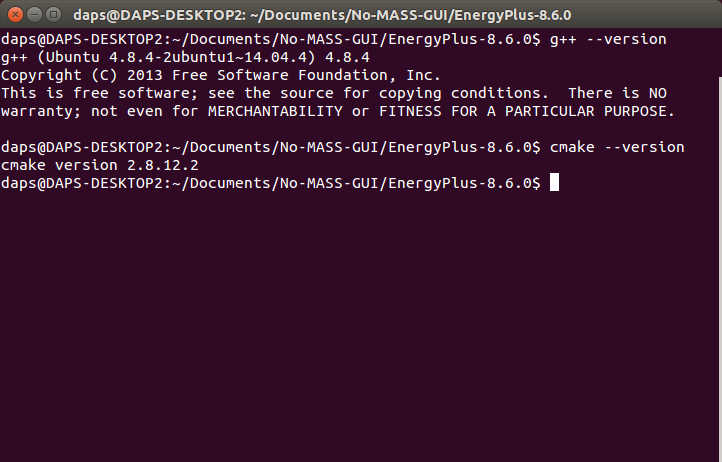
\includegraphics[width=10cm]{gcompiler_cmake_version.png}
\doxyfigcaption{g++ compiler and cmake installed versions}
\end{DoxyImage}

\item Navigate in the terminal to the root of the Energy\+Plus source code folder and create the build folder where the code will be compiled. 
\begin{DoxyCode}
cd /home/daps/Documents/No-MASS-GUI/EnergyPlus-8.6.0
mkdir build
cd build
\end{DoxyCode}

\item Launch C\+Make from the build location by executing the following command from terminal. 
\begin{DoxyCode}
ccmake ../
\end{DoxyCode}
 where {\ttfamily ../} referes to the build\textquotesingle{}s parent folder (root folder).
\item Configure the build by pressing {\itshape {\bfseries c}}, and a list of editable build options will be presented. Set the C\+M\+A\+K\+E\+\_\+\+B\+U\+I\+L\+D\+\_\+\+T\+Y\+PE type to \char`\"{}\+Release\char`\"{} and turn on the B\+U\+I\+L\+D\+\_\+\+F\+O\+R\+T\+R\+AN options at this step. Press {\itshape {\bfseries c}} again to reconfigure after completing changes, then {\itshape {\bfseries g}} to generate makefiles and exit. 
\begin{DoxyImage}
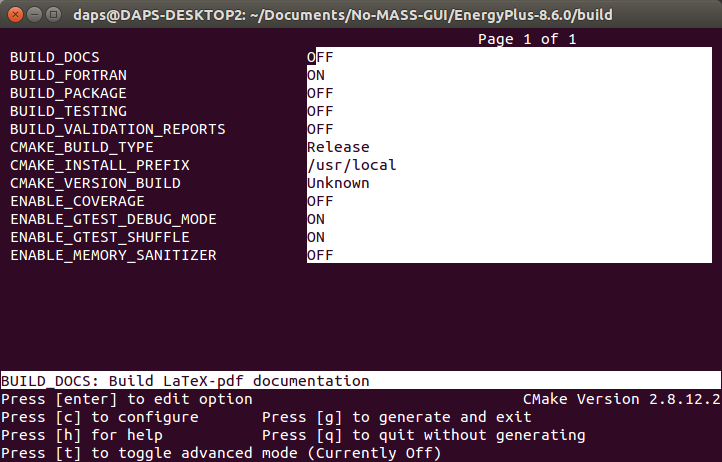
\includegraphics[width=10cm]{ccmake_gui_step2.png}
\doxyfigcaption{Build options}
\end{DoxyImage}
  
\item Finally, run {\ttfamily make -\/j N}, where {\ttfamily N} is the number of job slots to execute multiple jobs at once. The default number of job slots is one, which means one job at time. The number of job slots depends on the available hardware resources (C\+PU cores and memory), and the memory required by each make job. 
\begin{DoxyImage}
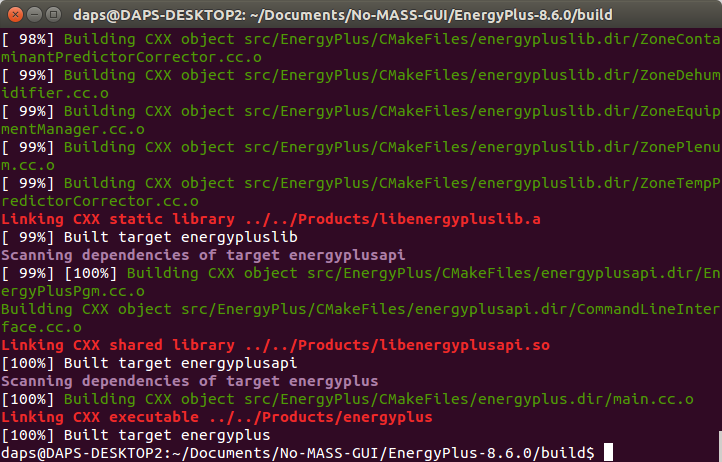
\includegraphics[width=10cm]{make_output.png}
\doxyfigcaption{`make -\/j 2` output}
\end{DoxyImage}
  
\item The compiled Energy\+Plus can be found in the {\ttfamily build/\+Products} folder. 
\begin{DoxyImage}
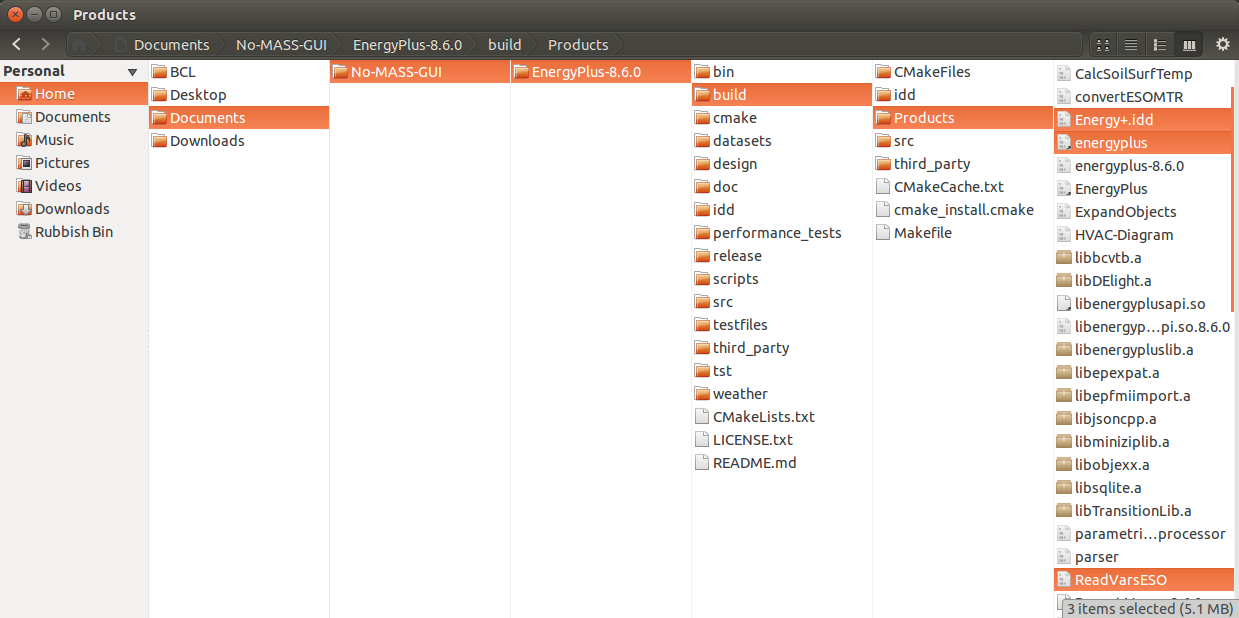
\includegraphics[width=15cm]{EPlus_exeFolder.png}
\doxyfigcaption{Energy\+Plus and Read\+Vars\+E\+SO applications folder}
\end{DoxyImage}
  
\end{DoxyEnumerate}



 

\subsection*{Compiling on Windows}



The compilation process followed in this guide is based on Visual Studio. The code can also be compiled using G\+CC. although the process is no included in this guide.


\begin{DoxyEnumerate}
\item Install Visual Studio. Visual Studio Community is distributed by Microsoft and free to use. Select the {\ttfamily Desktop development with C++} workload from the main window options and click install. 
\begin{DoxyImage}
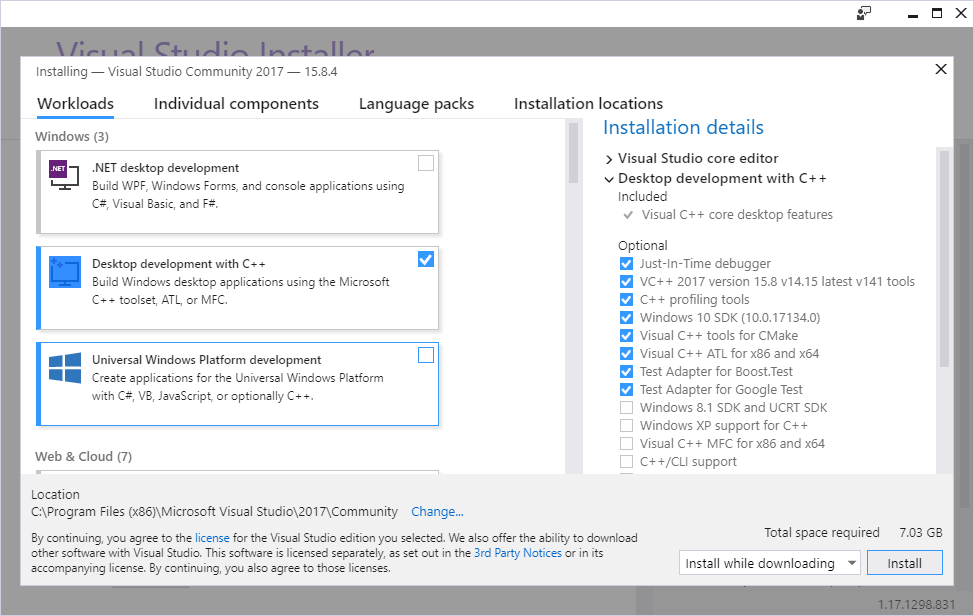
\includegraphics[width=15cm]{VSC2017_step1.png}
\doxyfigcaption{Visual Studio Community 2017}
\end{DoxyImage}
  
\item Install Python 2. It can be downloaded at \href{https://www.python.org/downloads/}{\tt https\+://www.\+python.\+org/downloads}
\item Install cmake that includes a graphic user interface (cmake-\/gui). Cmake can be downloaded at \href{https://cmake.org/download/}{\tt https\+://cmake.\+org/download}.
\item Install Min\+GW -\/ Minimalist G\+NU for Windows to support Fortran utilities. Min\+GW for Windows can be downloaded at \href{http://mingw-w64.org/doku.php/download}{\tt http\+://mingw-\/w64.\+org/doku.\+php/download}. 
\begin{DoxyImage}
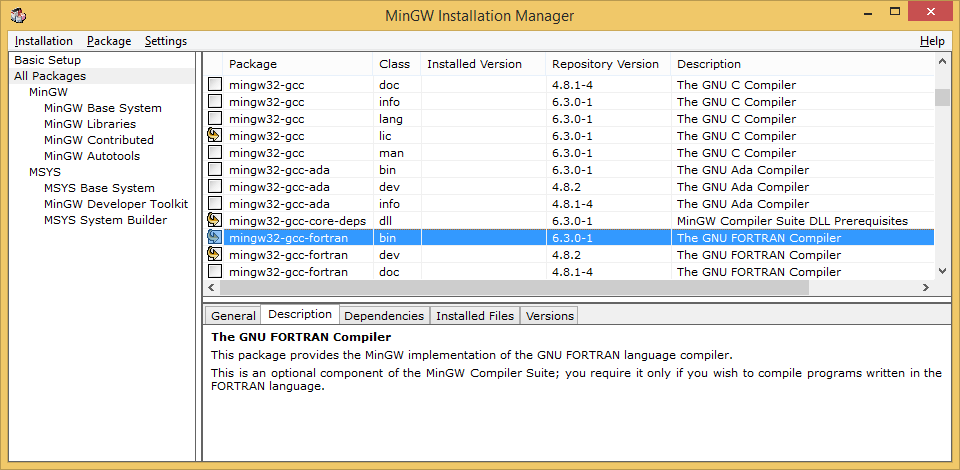
\includegraphics[width=15cm]{mingw64_selectoptions.png}
\doxyfigcaption{Min\+GW with Fortran support}
\end{DoxyImage}
  
\item Open {\ttfamily C\+Make (cmake-\/gui)}, point the {\ttfamily source code} to the root folder of the Energy\+Plus code and the {\ttfamily build} folder to the location inside the root folder. 
\begin{DoxyImage}
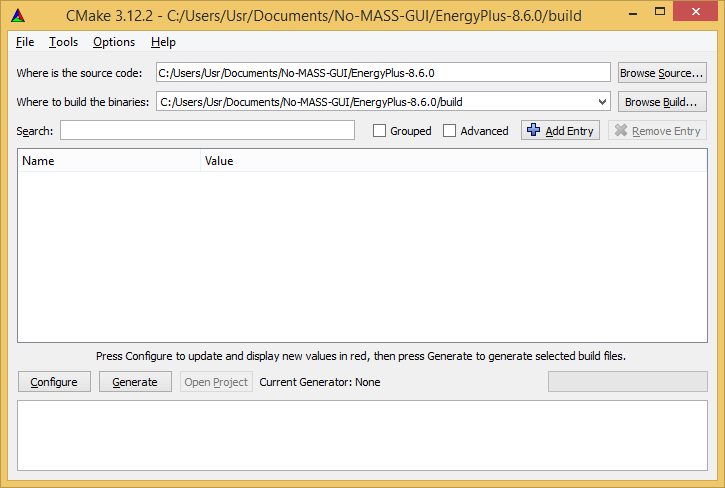
\includegraphics[width=15cm]{win_cmake_step1.png}
\doxyfigcaption{C\+Make-\/\+G\+UI}
\end{DoxyImage}
  
\item Click {\ttfamily Configure} and choose {\ttfamily Visual Studio 15} or {\ttfamily Visual Studio 15 Win64}. 
\begin{DoxyImage}
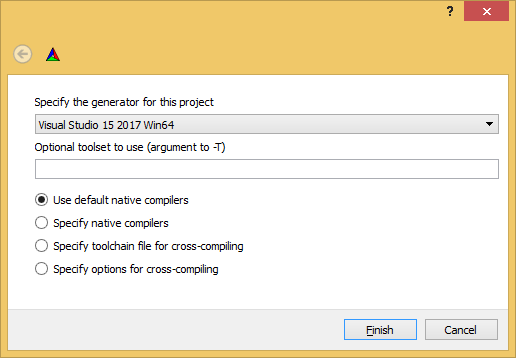
\includegraphics[width=8cm]{win_cmake_step2.png}
\doxyfigcaption{C\+Make-\/\+G\+UI configuration}
\end{DoxyImage}
  
\item Enable the {\ttfamily B\+U\+I\+L\+D\+\_\+\+F\+O\+R\+T\+R\+AN} option, then click {\ttfamily Generate} to produce a Visual Studio solution. 
\begin{DoxyImage}
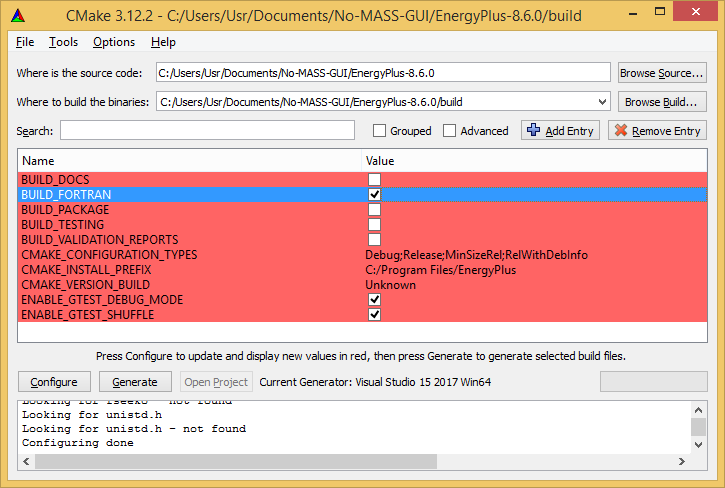
\includegraphics[width=15cm]{win_cmake_step3.png}
\doxyfigcaption{C\+Make-\/\+G\+UI generate Visual Studio solution}
\end{DoxyImage}
  
\item Open the solution in Visual Studio, select the build type to {\ttfamily Release} and compile the solution from the menu {\ttfamily Build/\+Build Solution}. 
\begin{DoxyImage}
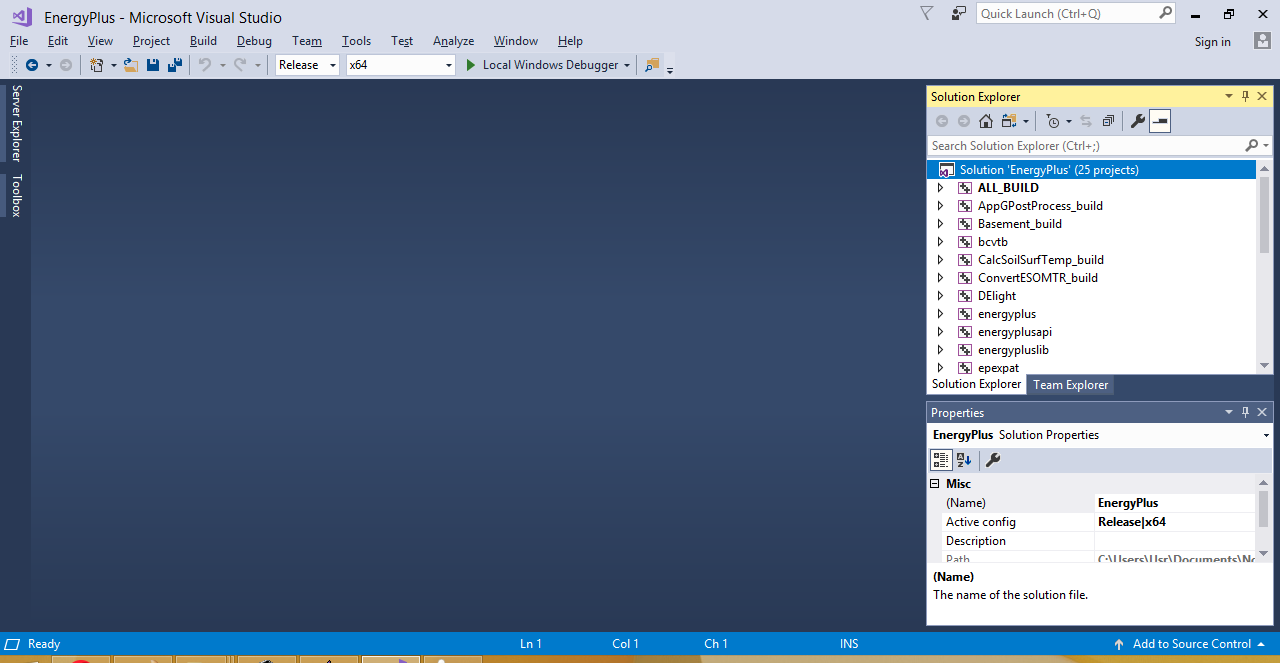
\includegraphics[width=15cm]{vs_compilerelease.png}
\doxyfigcaption{Release build compilation}
\end{DoxyImage}
  
\item The compiled Energy\+Plus can be found in the {\ttfamily build/\+Products/\+Release} folder. 
\begin{DoxyImage}
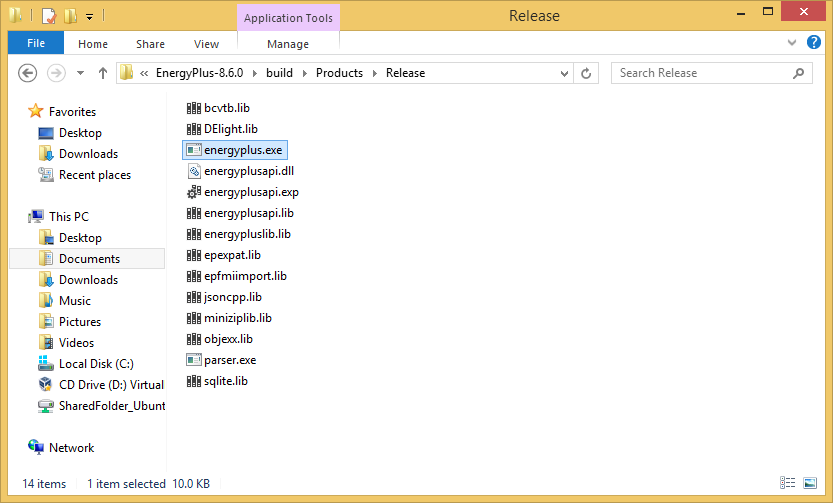
\includegraphics[width=15cm]{vs_compilerelease3.png}
\doxyfigcaption{Energy\+Plus.exe applications folder}
\end{DoxyImage}
  
\item Finally, copy the {\ttfamily Energy+.idd} file from {\ttfamily Products} to {\ttfamily Products/\+Release} folder.
\end{DoxyEnumerate}

 
\chapter{Prerequisites}
\label{_prerequisites}
\Hypertarget{_prerequisites}


No-\/\+M\+A\+S\+S-\/\+G\+UI is an application coded in Python. Therefore, a Python interpreter is required to launch the application. There are multiple Python interpreters for both Linux and Windows operating systems. Anaconda2 is an open source platform that integrates the Python compiler and data science and machine learning libraries. Using Anaconda simplify installation of extra packages required by the No-\/\+M\+A\+S\+S-\/\+G\+UI application. Anaconda2 (for Python 2.\+7) has been used to test the No-\/\+M\+A\+S\+S-\/\+G\+UI, and the installer can be downloaded from \href{https://www.anaconda.com/download/}{\tt https\+://www.\+anaconda.\+com/download}.

 

\subsection*{Spyder}

 Spyder (Scientific Python Development Envi\+Ronment) is a programming environment for Python included in Anaconda installation. The No-\/\+M\+A\+S\+S-\/\+G\+UI can be edited and launched from Spyder. 
\chapter{Implementation}
\label{_implementation}
\Hypertarget{_implementation}


This chapter describes the use of the No-\/\+M\+A\+S\+S-\/\+G\+UI to launch building performance simulations with integration of the No-\/\+M\+A\+SS platform. No-\/\+M\+A\+S\+S-\/\+G\+UI is coded in Python. Therefore, a Python interpreter is required to launch the application. There are multiple Python interpreters for both Llinux and Windows operating systems.

Anaconda2 is an open source platform that integrates Python and data science and machine learning libraries. (for Python 2.\+7)

 

\subsection*{Configuration}

 Lorem Ipsum is simply dummy text of the printing and typesetting industry. Lorem Ipsum has been the industry\textquotesingle{}s standard dummy text ever since the 1500s, when an unknown printer took a galley of type and scrambled it to make a type specimen book. It has survived not only five centuries, but also the leap into electronic typesetting, remaining essentially unchanged. It was popularised in the 1960s with the release of Letraset sheets containing Lorem Ipsum passages, and more recently with desktop publishing software like Aldus Page\+Maker including versions of Lorem Ipsum.

 

\subsubsection*{Simulation}

 Lorem Ipsum is simply dummy text of the printing and typesetting industry. Lorem Ipsum has been the industry\textquotesingle{}s standard dummy text ever since the 1500s, when an unknown printer took a galley of type and scrambled it to make a type specimen book. It has survived not only five centuries, but also the leap into electronic typesetting, remaining essentially unchanged. It was popularised in the 1960s with the release of Letraset sheets containing Lorem Ipsum passages, and more recently with desktop publishing software like Aldus Page\+Maker including versions of Lorem Ipsum.

 

\subsubsection*{Building}

 Lorem Ipsum is simply dummy text of the printing and typesetting industry. Lorem Ipsum has been the industry\textquotesingle{}s standard dummy text ever since the 1500s, when an unknown printer took a galley of type and scrambled it to make a type specimen book. It has survived not only five centuries, but also the leap into electronic typesetting, remaining essentially unchanged. It was popularised in the 1960s with the release of Letraset sheets containing Lorem Ipsum passages, and more recently with desktop publishing software like Aldus Page\+Maker including versions of Lorem Ipsum.

 

\paragraph*{Zones}

 Lorem Ipsum is simply dummy text of the printing and typesetting industry. Lorem Ipsum has been the industry\textquotesingle{}s standard dummy text ever since the 1500s, when an unknown printer took a galley of type and scrambled it to make a type specimen book. It has survived not only five centuries, but also the leap into electronic typesetting, remaining essentially unchanged. It was popularised in the 1960s with the release of Letraset sheets containing Lorem Ipsum passages, and more recently with desktop publishing software like Aldus Page\+Maker including versions of Lorem Ipsum.

 

\paragraph*{Agents}

 Lorem Ipsum is simply dummy text of the printing and typesetting industry. Lorem Ipsum has been the industry\textquotesingle{}s standard dummy text ever since the 1500s, when an unknown printer took a galley of type and scrambled it to make a type specimen book. It has survived not only five centuries, but also the leap into electronic typesetting, remaining essentially unchanged. It was popularised in the 1960s with the release of Letraset sheets containing Lorem Ipsum passages, and more recently with desktop publishing software like Aldus Page\+Maker including versions of Lorem Ipsum.

 

\subsubsection*{M\+A\+S\+S-\/\+Models}

 Lorem Ipsum is simply dummy text of the printing and typesetting industry. Lorem Ipsum has been the industry\textquotesingle{}s standard dummy text ever since the 1500s, when an unknown printer took a galley of type and scrambled it to make a type specimen book. It has survived not only five centuries, but also the leap into electronic typesetting, remaining essentially unchanged. It was popularised in the 1960s with the release of Letraset sheets containing Lorem Ipsum passages, and more recently with desktop publishing software like Aldus Page\+Maker including versions of Lorem Ipsum.

 

\subsection*{Launch Simulation Replicates}

 Lorem Ipsum is simply dummy text of the printing and typesetting industry. Lorem Ipsum has been the industry\textquotesingle{}s standard dummy text ever since the 1500s, when an unknown printer took a galley of type and scrambled it to make a type specimen book. It has survived not only five centuries, but also the leap into electronic typesetting, remaining essentially unchanged. It was popularised in the 1960s with the release of Letraset sheets containing Lorem Ipsum passages, and more recently with desktop publishing software like Aldus Page\+Maker including versions of Lorem Ipsum.

 

\subsection*{Plots}

 Lorem Ipsum is simply dummy text of the printing and typesetting industry. Lorem Ipsum has been the industry\textquotesingle{}s standard dummy text ever since the 1500s, when an unknown printer took a galley of type and scrambled it to make a type specimen book. It has survived not only five centuries, but also the leap into electronic typesetting, remaining essentially unchanged. It was popularised in the 1960s with the release of Letraset sheets containing Lorem Ipsum passages, and more recently with desktop publishing software like Aldus Page\+Maker including versions of Lorem Ipsum.

 

\subsubsection*{Heating}

 Lorem Ipsum is simply dummy text of the printing and typesetting industry. Lorem Ipsum has been the industry\textquotesingle{}s standard dummy text ever since the 1500s, when an unknown printer took a galley of type and scrambled it to make a type specimen book. It has survived not only five centuries, but also the leap into electronic typesetting, remaining essentially unchanged. It was popularised in the 1960s with the release of Letraset sheets containing Lorem Ipsum passages, and more recently with desktop publishing software like Aldus Page\+Maker including versions of Lorem Ipsum.

 

\subsubsection*{Cooling}

 Lorem Ipsum is simply dummy text of the printing and typesetting industry. Lorem Ipsum has been the industry\textquotesingle{}s standard dummy text ever since the 1500s, when an unknown printer took a galley of type and scrambled it to make a type specimen book. It has survived not only five centuries, but also the leap into electronic typesetting, remaining essentially unchanged. It was popularised in the 1960s with the release of Letraset sheets containing Lorem Ipsum passages, and more recently with desktop publishing software like Aldus Page\+Maker including versions of Lorem Ipsum.

 

\subsubsection*{Interactions}

 Lorem Ipsum is simply dummy text of the printing and typesetting industry. Lorem Ipsum has been the industry\textquotesingle{}s standard dummy text ever since the 1500s, when an unknown printer took a galley of type and scrambled it to make a type specimen book. It has survived not only five centuries, but also the leap into electronic typesetting, remaining essentially unchanged. It was popularised in the 1960s with the release of Letraset sheets containing Lorem Ipsum passages, and more recently with desktop publishing software like Aldus Page\+Maker including versions of Lorem Ipsum. 
\chapter{Hierarchical Index}
\section{Class Hierarchy}
This inheritance list is sorted roughly, but not completely, alphabetically\+:\begin{DoxyCompactList}
\item \contentsline{section}{App}{\pageref{class_no_m_a_s_s___g_u_i_1_1_app}}{}
\item Combobox\begin{DoxyCompactList}
\item \contentsline{section}{Utils.\+U\+I.\+Controls.\+Cascading\+Drop\+Down\+List}{\pageref{class_c_utils_1_1_utils_1_1_u_i_1_1_controls_1_1_cascading_drop_down_list}}{}
\item \contentsline{section}{Utils.\+U\+I.\+Controls.\+Drop\+Down\+List}{\pageref{class_c_utils_1_1_utils_1_1_u_i_1_1_controls_1_1_drop_down_list}}{}
\end{DoxyCompactList}
\item \contentsline{section}{Utils.\+Config}{\pageref{class_c_utils_1_1_utils_1_1_config}}{}
\item \contentsline{section}{Utils.\+Constants}{\pageref{class_c_utils_1_1_utils_1_1_constants}}{}
\item \contentsline{section}{Utils.\+U\+I.\+Controls}{\pageref{class_c_utils_1_1_utils_1_1_u_i_1_1_controls}}{}
\item Frame\begin{DoxyCompactList}
\item \contentsline{section}{Utils.\+U\+I.\+Controls.\+Collapsible\+Frame}{\pageref{class_c_utils_1_1_utils_1_1_u_i_1_1_controls_1_1_collapsible_frame}}{}
\item \contentsline{section}{Utils.\+U\+I.\+Controls.\+Scrollable\+Container}{\pageref{class_c_utils_1_1_utils_1_1_u_i_1_1_controls_1_1_scrollable_container}}{}
\end{DoxyCompactList}
\item \contentsline{section}{Utils.\+Functions}{\pageref{class_c_utils_1_1_utils_1_1_functions}}{}
\item \contentsline{section}{Utils.\+Resources.\+Icons}{\pageref{class_c_utils_1_1_utils_1_1_resources_1_1_icons}}{}
\item \contentsline{section}{Utils.\+IO}{\pageref{class_c_utils_1_1_utils_1_1_i_o}}{}
\item Listbox\begin{DoxyCompactList}
\item \contentsline{section}{Utils.\+U\+I.\+Controls.\+Lst\+Box}{\pageref{class_c_utils_1_1_utils_1_1_u_i_1_1_controls_1_1_lst_box}}{}
\end{DoxyCompactList}
\item object\begin{DoxyCompactList}
\item \contentsline{section}{C\+Building}{\pageref{class_c_building_1_1_c_building}}{}
\item \contentsline{section}{C\+Lights}{\pageref{class_c_lights_1_1_c_lights}}{}
\item \contentsline{section}{C\+Occupant}{\pageref{class_c_occupant_1_1_c_occupant}}{}
\item \contentsline{section}{C\+Occupant\+Template}{\pageref{class_c_occupant_template_1_1_c_occupant_template}}{}
\item \contentsline{section}{C\+Presence}{\pageref{class_c_presence_1_1_c_presence}}{}
\item \contentsline{section}{C\+Shade}{\pageref{class_c_shade_1_1_c_shade}}{}
\item \contentsline{section}{C\+Shades}{\pageref{class_c_shades_1_1_c_shades}}{}
\item \contentsline{section}{Simulation}{\pageref{class_c_simulation_1_1_simulation}}{}
\item \contentsline{section}{Simulation.\+Building}{\pageref{class_c_simulation_1_1_simulation_1_1_building}}{}
\item \contentsline{section}{Simulation.\+Building.\+Occupant}{\pageref{class_c_simulation_1_1_simulation_1_1_building_1_1_occupant}}{}
\item \contentsline{section}{Simulation.\+Building.\+Occupant.\+Profile}{\pageref{class_c_simulation_1_1_simulation_1_1_building_1_1_occupant_1_1_profile}}{}
\item \contentsline{section}{Simulation.\+Building.\+Zone}{\pageref{class_c_simulation_1_1_simulation_1_1_building_1_1_zone}}{}
\item \contentsline{section}{Simulation.\+No\+M\+A\+S\+S\+Models}{\pageref{class_c_simulation_1_1_simulation_1_1_no_m_a_s_s_models}}{}
\item \contentsline{section}{Simulation.\+No\+M\+A\+S\+S\+Models.\+Agent\+Heat\+Gains}{\pageref{class_c_simulation_1_1_simulation_1_1_no_m_a_s_s_models_1_1_agent_heat_gains}}{}
\item \contentsline{section}{Simulation.\+No\+M\+A\+S\+S\+Models.\+Heating}{\pageref{class_c_simulation_1_1_simulation_1_1_no_m_a_s_s_models_1_1_heating}}{}
\item \contentsline{section}{Simulation.\+No\+M\+A\+S\+S\+Models.\+Lights}{\pageref{class_c_simulation_1_1_simulation_1_1_no_m_a_s_s_models_1_1_lights}}{}
\item \contentsline{section}{Simulation.\+No\+M\+A\+S\+S\+Models.\+Presence}{\pageref{class_c_simulation_1_1_simulation_1_1_no_m_a_s_s_models_1_1_presence}}{}
\item \contentsline{section}{Simulation.\+No\+M\+A\+S\+S\+Models.\+Shades}{\pageref{class_c_simulation_1_1_simulation_1_1_no_m_a_s_s_models_1_1_shades}}{}
\item \contentsline{section}{Simulation.\+No\+M\+A\+S\+S\+Models.\+Shades.\+Shade}{\pageref{class_c_simulation_1_1_simulation_1_1_no_m_a_s_s_models_1_1_shades_1_1_shade}}{}
\item \contentsline{section}{Simulation.\+No\+M\+A\+S\+S\+Models.\+Windows}{\pageref{class_c_simulation_1_1_simulation_1_1_no_m_a_s_s_models_1_1_windows}}{}
\item \contentsline{section}{Simulation.\+No\+M\+A\+S\+S\+Models.\+Windows.\+Window}{\pageref{class_c_simulation_1_1_simulation_1_1_no_m_a_s_s_models_1_1_windows_1_1_window}}{}
\item \contentsline{section}{Utils.\+U\+I.\+Controls.\+Auto\+Scroll\+Container}{\pageref{class_c_utils_1_1_utils_1_1_u_i_1_1_controls_1_1_auto_scroll_container}}{}
\begin{DoxyCompactList}
\item \contentsline{section}{Utils.\+U\+I.\+Controls.\+Scrolled\+Tree\+View}{\pageref{class_c_utils_1_1_utils_1_1_u_i_1_1_controls_1_1_scrolled_tree_view}}{}
\end{DoxyCompactList}
\item \contentsline{section}{Utils.\+U\+I.\+Controls.\+Cascading\+Drop\+Down\+List}{\pageref{class_c_utils_1_1_utils_1_1_u_i_1_1_controls_1_1_cascading_drop_down_list}}{}
\item \contentsline{section}{Utils.\+U\+I.\+Controls.\+Collapsible\+Frame}{\pageref{class_c_utils_1_1_utils_1_1_u_i_1_1_controls_1_1_collapsible_frame}}{}
\item \contentsline{section}{Utils.\+U\+I.\+Controls.\+Drop\+Down\+List}{\pageref{class_c_utils_1_1_utils_1_1_u_i_1_1_controls_1_1_drop_down_list}}{}
\item \contentsline{section}{Utils.\+U\+I.\+Controls.\+Lst\+Box}{\pageref{class_c_utils_1_1_utils_1_1_u_i_1_1_controls_1_1_lst_box}}{}
\item \contentsline{section}{Utils.\+U\+I.\+Controls.\+Scrollable\+Container}{\pageref{class_c_utils_1_1_utils_1_1_u_i_1_1_controls_1_1_scrollable_container}}{}
\item \contentsline{section}{C\+Window}{\pageref{class_c_window_1_1_c_window}}{}
\item \contentsline{section}{C\+Windows}{\pageref{class_c_windows_1_1_c_windows}}{}
\item \contentsline{section}{C\+Zone}{\pageref{class_c_zone_1_1_c_zone}}{}
\item \contentsline{section}{Frm\+Building}{\pageref{class_f_building_1_1_frm_building}}{}
\item \contentsline{section}{Frm\+Configuration}{\pageref{class_f_configuration_1_1_frm_configuration}}{}
\item \contentsline{section}{Frm\+Empty}{\pageref{class_f_empty_1_1_frm_empty}}{}
\item \contentsline{section}{Frm\+Lights}{\pageref{class_f_lights_1_1_frm_lights}}{}
\item \contentsline{section}{Frm\+List\+Of\+Zones\+Verification}{\pageref{class_f_list_of_zones_verification_1_1_frm_list_of_zones_verification}}{}
\item \contentsline{section}{Frm\+Log}{\pageref{class_f_log_1_1_frm_log}}{}
\item \contentsline{section}{Frm\+Occupant}{\pageref{class_f_occupant_1_1_frm_occupant}}{}
\item \contentsline{section}{Frm\+Occupant\+Templates}{\pageref{class_f_occupant_templates_1_1_frm_occupant_templates}}{}
\item \contentsline{section}{Frm\+Plots}{\pageref{class_f_plots_1_1_frm_plots}}{}
\item \contentsline{section}{Frm\+Presence}{\pageref{class_f_presence_1_1_frm_presence}}{}
\item \contentsline{section}{Frm\+Run}{\pageref{class_f_run_1_1_frm_run}}{}
\item \contentsline{section}{Frm\+Shade}{\pageref{class_f_shade_1_1_frm_shade}}{}
\item \contentsline{section}{Frm\+Shades}{\pageref{class_f_shades_1_1_frm_shades}}{}
\item \contentsline{section}{Frm\+Window}{\pageref{class_f_window_1_1_frm_window}}{}
\item \contentsline{section}{Frm\+Windows}{\pageref{class_f_windows_1_1_frm_windows}}{}
\item \contentsline{section}{Frm\+Zone}{\pageref{class_f_zone_1_1_frm_zone}}{}
\end{DoxyCompactList}
\item \contentsline{section}{Utils.\+Resources}{\pageref{class_c_utils_1_1_utils_1_1_resources}}{}
\item \contentsline{section}{Tool\+Tip}{\pageref{class_c_tool_tip_1_1_tool_tip}}{}
\item Treeview\begin{DoxyCompactList}
\item \contentsline{section}{Utils.\+U\+I.\+Controls.\+Scrolled\+Tree\+View}{\pageref{class_c_utils_1_1_utils_1_1_u_i_1_1_controls_1_1_scrolled_tree_view}}{}
\end{DoxyCompactList}
\item \contentsline{section}{Utils.\+UI}{\pageref{class_c_utils_1_1_utils_1_1_u_i}}{}
\item \contentsline{section}{Utils}{\pageref{class_c_utils_1_1_utils}}{}
\item \contentsline{section}{Utils.\+X\+ML}{\pageref{class_c_utils_1_1_utils_1_1_x_m_l}}{}
\end{DoxyCompactList}

\chapter{Class Index}
\section{Class List}
Here are the classes, structs, unions and interfaces with brief descriptions\+:\begin{DoxyCompactList}
\item\contentsline{section}{\hyperlink{class_c_simulation_1_1_simulation_1_1_no_m_a_s_s_models_1_1_agent_heat_gains}{Simulation.\+No\+M\+A\+S\+S\+Models.\+Agent\+Heat\+Gains} }{\pageref{class_c_simulation_1_1_simulation_1_1_no_m_a_s_s_models_1_1_agent_heat_gains}}{}
\item\contentsline{section}{\hyperlink{class_no_m_a_s_s___g_u_i_1_1_app}{App} }{\pageref{class_no_m_a_s_s___g_u_i_1_1_app}}{}
\item\contentsline{section}{\hyperlink{class_c_utils_1_1_utils_1_1_u_i_1_1_controls_1_1_auto_scroll_container}{Utils.\+U\+I.\+Controls.\+Auto\+Scroll\+Container} }{\pageref{class_c_utils_1_1_utils_1_1_u_i_1_1_controls_1_1_auto_scroll_container}}{}
\item\contentsline{section}{\hyperlink{class_c_simulation_1_1_simulation_1_1_building}{Simulation.\+Building} }{\pageref{class_c_simulation_1_1_simulation_1_1_building}}{}
\item\contentsline{section}{\hyperlink{class_c_utils_1_1_utils_1_1_u_i_1_1_controls_1_1_cascading_drop_down_list}{Utils.\+U\+I.\+Controls.\+Cascading\+Drop\+Down\+List} }{\pageref{class_c_utils_1_1_utils_1_1_u_i_1_1_controls_1_1_cascading_drop_down_list}}{}
\item\contentsline{section}{\hyperlink{class_c_building_1_1_c_building}{C\+Building} }{\pageref{class_c_building_1_1_c_building}}{}
\item\contentsline{section}{\hyperlink{class_c_lights_1_1_c_lights}{C\+Lights} }{\pageref{class_c_lights_1_1_c_lights}}{}
\item\contentsline{section}{\hyperlink{class_c_occupant_1_1_c_occupant}{C\+Occupant} }{\pageref{class_c_occupant_1_1_c_occupant}}{}
\item\contentsline{section}{\hyperlink{class_c_occupant_template_1_1_c_occupant_template}{C\+Occupant\+Template} }{\pageref{class_c_occupant_template_1_1_c_occupant_template}}{}
\item\contentsline{section}{\hyperlink{class_c_utils_1_1_utils_1_1_u_i_1_1_controls_1_1_collapsible_frame}{Utils.\+U\+I.\+Controls.\+Collapsible\+Frame} }{\pageref{class_c_utils_1_1_utils_1_1_u_i_1_1_controls_1_1_collapsible_frame}}{}
\item\contentsline{section}{\hyperlink{class_c_utils_1_1_utils_1_1_config}{Utils.\+Config} }{\pageref{class_c_utils_1_1_utils_1_1_config}}{}
\item\contentsline{section}{\hyperlink{class_c_utils_1_1_utils_1_1_constants}{Utils.\+Constants} }{\pageref{class_c_utils_1_1_utils_1_1_constants}}{}
\item\contentsline{section}{\hyperlink{class_c_utils_1_1_utils_1_1_u_i_1_1_controls}{Utils.\+U\+I.\+Controls} }{\pageref{class_c_utils_1_1_utils_1_1_u_i_1_1_controls}}{}
\item\contentsline{section}{\hyperlink{class_c_presence_1_1_c_presence}{C\+Presence} }{\pageref{class_c_presence_1_1_c_presence}}{}
\item\contentsline{section}{\hyperlink{class_c_shade_1_1_c_shade}{C\+Shade} }{\pageref{class_c_shade_1_1_c_shade}}{}
\item\contentsline{section}{\hyperlink{class_c_shades_1_1_c_shades}{C\+Shades} }{\pageref{class_c_shades_1_1_c_shades}}{}
\item\contentsline{section}{\hyperlink{class_c_window_1_1_c_window}{C\+Window} }{\pageref{class_c_window_1_1_c_window}}{}
\item\contentsline{section}{\hyperlink{class_c_windows_1_1_c_windows}{C\+Windows} }{\pageref{class_c_windows_1_1_c_windows}}{}
\item\contentsline{section}{\hyperlink{class_c_zone_1_1_c_zone}{C\+Zone} }{\pageref{class_c_zone_1_1_c_zone}}{}
\item\contentsline{section}{\hyperlink{class_c_utils_1_1_utils_1_1_u_i_1_1_controls_1_1_drop_down_list}{Utils.\+U\+I.\+Controls.\+Drop\+Down\+List} }{\pageref{class_c_utils_1_1_utils_1_1_u_i_1_1_controls_1_1_drop_down_list}}{}
\item\contentsline{section}{\hyperlink{class_f_building_1_1_frm_building}{Frm\+Building} }{\pageref{class_f_building_1_1_frm_building}}{}
\item\contentsline{section}{\hyperlink{class_f_configuration_1_1_frm_configuration}{Frm\+Configuration} }{\pageref{class_f_configuration_1_1_frm_configuration}}{}
\item\contentsline{section}{\hyperlink{class_f_empty_1_1_frm_empty}{Frm\+Empty} }{\pageref{class_f_empty_1_1_frm_empty}}{}
\item\contentsline{section}{\hyperlink{class_f_lights_1_1_frm_lights}{Frm\+Lights} }{\pageref{class_f_lights_1_1_frm_lights}}{}
\item\contentsline{section}{\hyperlink{class_f_list_of_zones_verification_1_1_frm_list_of_zones_verification}{Frm\+List\+Of\+Zones\+Verification} }{\pageref{class_f_list_of_zones_verification_1_1_frm_list_of_zones_verification}}{}
\item\contentsline{section}{\hyperlink{class_f_log_1_1_frm_log}{Frm\+Log} }{\pageref{class_f_log_1_1_frm_log}}{}
\item\contentsline{section}{\hyperlink{class_f_occupant_1_1_frm_occupant}{Frm\+Occupant} }{\pageref{class_f_occupant_1_1_frm_occupant}}{}
\item\contentsline{section}{\hyperlink{class_f_occupant_templates_1_1_frm_occupant_templates}{Frm\+Occupant\+Templates} }{\pageref{class_f_occupant_templates_1_1_frm_occupant_templates}}{}
\item\contentsline{section}{\hyperlink{class_f_plots_1_1_frm_plots}{Frm\+Plots} }{\pageref{class_f_plots_1_1_frm_plots}}{}
\item\contentsline{section}{\hyperlink{class_f_presence_1_1_frm_presence}{Frm\+Presence} }{\pageref{class_f_presence_1_1_frm_presence}}{}
\item\contentsline{section}{\hyperlink{class_f_run_1_1_frm_run}{Frm\+Run} }{\pageref{class_f_run_1_1_frm_run}}{}
\item\contentsline{section}{\hyperlink{class_f_shade_1_1_frm_shade}{Frm\+Shade} }{\pageref{class_f_shade_1_1_frm_shade}}{}
\item\contentsline{section}{\hyperlink{class_f_shades_1_1_frm_shades}{Frm\+Shades} }{\pageref{class_f_shades_1_1_frm_shades}}{}
\item\contentsline{section}{\hyperlink{class_f_window_1_1_frm_window}{Frm\+Window} }{\pageref{class_f_window_1_1_frm_window}}{}
\item\contentsline{section}{\hyperlink{class_f_windows_1_1_frm_windows}{Frm\+Windows} }{\pageref{class_f_windows_1_1_frm_windows}}{}
\item\contentsline{section}{\hyperlink{class_f_zone_1_1_frm_zone}{Frm\+Zone} }{\pageref{class_f_zone_1_1_frm_zone}}{}
\item\contentsline{section}{\hyperlink{class_c_utils_1_1_utils_1_1_functions}{Utils.\+Functions} }{\pageref{class_c_utils_1_1_utils_1_1_functions}}{}
\item\contentsline{section}{\hyperlink{class_c_simulation_1_1_simulation_1_1_no_m_a_s_s_models_1_1_heating}{Simulation.\+No\+M\+A\+S\+S\+Models.\+Heating} }{\pageref{class_c_simulation_1_1_simulation_1_1_no_m_a_s_s_models_1_1_heating}}{}
\item\contentsline{section}{\hyperlink{class_c_utils_1_1_utils_1_1_resources_1_1_icons}{Utils.\+Resources.\+Icons} }{\pageref{class_c_utils_1_1_utils_1_1_resources_1_1_icons}}{}
\item\contentsline{section}{\hyperlink{class_c_utils_1_1_utils_1_1_i_o}{Utils.\+IO} }{\pageref{class_c_utils_1_1_utils_1_1_i_o}}{}
\item\contentsline{section}{\hyperlink{class_c_simulation_1_1_simulation_1_1_no_m_a_s_s_models_1_1_lights}{Simulation.\+No\+M\+A\+S\+S\+Models.\+Lights} }{\pageref{class_c_simulation_1_1_simulation_1_1_no_m_a_s_s_models_1_1_lights}}{}
\item\contentsline{section}{\hyperlink{class_c_utils_1_1_utils_1_1_u_i_1_1_controls_1_1_lst_box}{Utils.\+U\+I.\+Controls.\+Lst\+Box} }{\pageref{class_c_utils_1_1_utils_1_1_u_i_1_1_controls_1_1_lst_box}}{}
\item\contentsline{section}{\hyperlink{class_c_simulation_1_1_simulation_1_1_no_m_a_s_s_models}{Simulation.\+No\+M\+A\+S\+S\+Models} }{\pageref{class_c_simulation_1_1_simulation_1_1_no_m_a_s_s_models}}{}
\item\contentsline{section}{\hyperlink{class_c_simulation_1_1_simulation_1_1_building_1_1_occupant}{Simulation.\+Building.\+Occupant} }{\pageref{class_c_simulation_1_1_simulation_1_1_building_1_1_occupant}}{}
\item\contentsline{section}{\hyperlink{class_c_simulation_1_1_simulation_1_1_no_m_a_s_s_models_1_1_presence}{Simulation.\+No\+M\+A\+S\+S\+Models.\+Presence} }{\pageref{class_c_simulation_1_1_simulation_1_1_no_m_a_s_s_models_1_1_presence}}{}
\item\contentsline{section}{\hyperlink{class_c_simulation_1_1_simulation_1_1_building_1_1_occupant_1_1_profile}{Simulation.\+Building.\+Occupant.\+Profile} }{\pageref{class_c_simulation_1_1_simulation_1_1_building_1_1_occupant_1_1_profile}}{}
\item\contentsline{section}{\hyperlink{class_c_utils_1_1_utils_1_1_resources}{Utils.\+Resources} }{\pageref{class_c_utils_1_1_utils_1_1_resources}}{}
\item\contentsline{section}{\hyperlink{class_c_utils_1_1_utils_1_1_u_i_1_1_controls_1_1_scrollable_container}{Utils.\+U\+I.\+Controls.\+Scrollable\+Container} }{\pageref{class_c_utils_1_1_utils_1_1_u_i_1_1_controls_1_1_scrollable_container}}{}
\item\contentsline{section}{\hyperlink{class_c_utils_1_1_utils_1_1_u_i_1_1_controls_1_1_scrolled_tree_view}{Utils.\+U\+I.\+Controls.\+Scrolled\+Tree\+View} }{\pageref{class_c_utils_1_1_utils_1_1_u_i_1_1_controls_1_1_scrolled_tree_view}}{}
\item\contentsline{section}{\hyperlink{class_c_simulation_1_1_simulation_1_1_no_m_a_s_s_models_1_1_shades_1_1_shade}{Simulation.\+No\+M\+A\+S\+S\+Models.\+Shades.\+Shade} }{\pageref{class_c_simulation_1_1_simulation_1_1_no_m_a_s_s_models_1_1_shades_1_1_shade}}{}
\item\contentsline{section}{\hyperlink{class_c_simulation_1_1_simulation_1_1_no_m_a_s_s_models_1_1_shades}{Simulation.\+No\+M\+A\+S\+S\+Models.\+Shades} }{\pageref{class_c_simulation_1_1_simulation_1_1_no_m_a_s_s_models_1_1_shades}}{}
\item\contentsline{section}{\hyperlink{class_c_simulation_1_1_simulation}{Simulation} }{\pageref{class_c_simulation_1_1_simulation}}{}
\item\contentsline{section}{\hyperlink{class_c_tool_tip_1_1_tool_tip}{Tool\+Tip} }{\pageref{class_c_tool_tip_1_1_tool_tip}}{}
\item\contentsline{section}{\hyperlink{class_c_utils_1_1_utils_1_1_u_i}{Utils.\+UI} }{\pageref{class_c_utils_1_1_utils_1_1_u_i}}{}
\item\contentsline{section}{\hyperlink{class_c_utils_1_1_utils}{Utils} }{\pageref{class_c_utils_1_1_utils}}{}
\item\contentsline{section}{\hyperlink{class_c_simulation_1_1_simulation_1_1_no_m_a_s_s_models_1_1_windows_1_1_window}{Simulation.\+No\+M\+A\+S\+S\+Models.\+Windows.\+Window} }{\pageref{class_c_simulation_1_1_simulation_1_1_no_m_a_s_s_models_1_1_windows_1_1_window}}{}
\item\contentsline{section}{\hyperlink{class_c_simulation_1_1_simulation_1_1_no_m_a_s_s_models_1_1_windows}{Simulation.\+No\+M\+A\+S\+S\+Models.\+Windows} }{\pageref{class_c_simulation_1_1_simulation_1_1_no_m_a_s_s_models_1_1_windows}}{}
\item\contentsline{section}{\hyperlink{class_c_utils_1_1_utils_1_1_x_m_l}{Utils.\+X\+ML} }{\pageref{class_c_utils_1_1_utils_1_1_x_m_l}}{}
\item\contentsline{section}{\hyperlink{class_c_simulation_1_1_simulation_1_1_building_1_1_zone}{Simulation.\+Building.\+Zone} }{\pageref{class_c_simulation_1_1_simulation_1_1_building_1_1_zone}}{}
\end{DoxyCompactList}

\chapter{Class Documentation}
\hypertarget{class_c_simulation_1_1_simulation_1_1_no_m_a_s_s_models_1_1_agent_heat_gains}{}\section{Simulation.\+No\+M\+A\+S\+S\+Models.\+Agent\+Heat\+Gains Class Reference}
\label{class_c_simulation_1_1_simulation_1_1_no_m_a_s_s_models_1_1_agent_heat_gains}\index{Simulation.\+No\+M\+A\+S\+S\+Models.\+Agent\+Heat\+Gains@{Simulation.\+No\+M\+A\+S\+S\+Models.\+Agent\+Heat\+Gains}}
Inheritance diagram for Simulation.\+No\+M\+A\+S\+S\+Models.\+Agent\+Heat\+Gains\+:\begin{figure}[H]
\begin{center}
\leavevmode
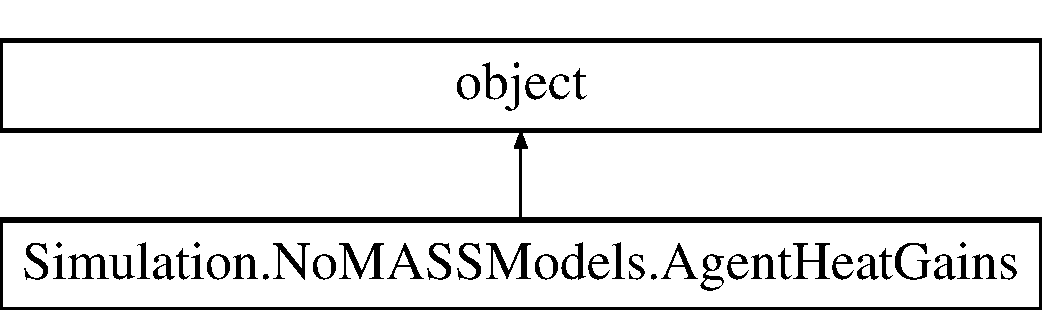
\includegraphics[height=2.000000cm]{class_c_simulation_1_1_simulation_1_1_no_m_a_s_s_models_1_1_agent_heat_gains}
\end{center}
\end{figure}
\subsection*{Public Member Functions}
\begin{DoxyCompactItemize}
\item 
\mbox{\Hypertarget{class_c_simulation_1_1_simulation_1_1_no_m_a_s_s_models_1_1_agent_heat_gains_ae64f0875afe3067b97ba370b354b9213}\label{class_c_simulation_1_1_simulation_1_1_no_m_a_s_s_models_1_1_agent_heat_gains_ae64f0875afe3067b97ba370b354b9213}} 
def {\bfseries \+\_\+\+\_\+init\+\_\+\+\_\+} (self)
\end{DoxyCompactItemize}
\subsection*{Public Attributes}
\begin{DoxyCompactItemize}
\item 
\mbox{\Hypertarget{class_c_simulation_1_1_simulation_1_1_no_m_a_s_s_models_1_1_agent_heat_gains_a91b39549c797bd5646357c8b6eecad0f}\label{class_c_simulation_1_1_simulation_1_1_no_m_a_s_s_models_1_1_agent_heat_gains_a91b39549c797bd5646357c8b6eecad0f}} 
{\bfseries enabled}
\end{DoxyCompactItemize}


\subsection{Detailed Description}


Definition at line 168 of file C\+Simulation.\+py.



The documentation for this class was generated from the following file\+:\begin{DoxyCompactItemize}
\item 
C\+Simulation.\+py\end{DoxyCompactItemize}

\hypertarget{class_no_m_a_s_s___g_u_i_1_1_app}{}\section{App Class Reference}
\label{class_no_m_a_s_s___g_u_i_1_1_app}\index{App@{App}}
\subsection*{Public Member Functions}
\begin{DoxyCompactItemize}
\item 
def \hyperlink{class_no_m_a_s_s___g_u_i_1_1_app_aa2c521b1919bad17bbd98c40cf56a7d4}{create\+Main\+Toolbar} (self, parent)
\begin{DoxyCompactList}\small\item\em Create main tool bar Create the main tool bar. \end{DoxyCompactList}\item 
def \hyperlink{class_no_m_a_s_s___g_u_i_1_1_app_ab88dd8d1817c2c1026001f3aa25ac355}{create\+Status\+Bar} (self, parent)
\begin{DoxyCompactList}\small\item\em Create status bar Create status. \end{DoxyCompactList}\item 
def \hyperlink{class_no_m_a_s_s___g_u_i_1_1_app_a49c1ac8804dc14c695793e23549756d7}{exit\+Callback} (self)
\begin{DoxyCompactList}\small\item\em Close application Destroy all resources before closing the application. \end{DoxyCompactList}\item 
def \hyperlink{class_no_m_a_s_s___g_u_i_1_1_app_a3fbca20a2bdf6d712baf7816a11c3585}{free\+Resources} (self)
\begin{DoxyCompactList}\small\item\em Destroy forms and widgets Destroy forms and widgets. \end{DoxyCompactList}\item 
def \hyperlink{class_no_m_a_s_s___g_u_i_1_1_app_abeee64cfa5bb453539b747213c594bbc}{reset\+Project} (self, load\+Default\+No\+M\+A\+S\+S\+Models=False)
\begin{DoxyCompactList}\small\item\em Reset data structures Reset data structures. \end{DoxyCompactList}\item 
def \hyperlink{class_no_m_a_s_s___g_u_i_1_1_app_ae1e47083122a73b7f4ad716b42f165a7}{new\+Project} (self)
\begin{DoxyCompactList}\small\item\em Create a new empty project Create a new empty project. \end{DoxyCompactList}\item 
\mbox{\Hypertarget{class_no_m_a_s_s___g_u_i_1_1_app_a5cb14c4329f786880ab70733cecf476c}\label{class_no_m_a_s_s___g_u_i_1_1_app_a5cb14c4329f786880ab70733cecf476c}} 
def {\bfseries refresh\+Tab\+Edit} (self, new\+Height=None)
\item 
def \hyperlink{class_no_m_a_s_s___g_u_i_1_1_app_a8027378f2d626f57d5832362b5712104}{open\+Project} (self)
\begin{DoxyCompactList}\small\item\em Open a project Open a project. \end{DoxyCompactList}\item 
def \hyperlink{class_no_m_a_s_s___g_u_i_1_1_app_a292a02cccaabec778b1dd648ac0aa146}{save\+Project} (self)
\begin{DoxyCompactList}\small\item\em Save current project Save current project. \end{DoxyCompactList}\item 
\mbox{\Hypertarget{class_no_m_a_s_s___g_u_i_1_1_app_ae3054086b72ee2f16401c9a937097cee}\label{class_no_m_a_s_s___g_u_i_1_1_app_ae3054086b72ee2f16401c9a937097cee}} 
def {\bfseries save\+Configuration} (self, filename, session\+ID=None)
\item 
\mbox{\Hypertarget{class_no_m_a_s_s___g_u_i_1_1_app_a04cdefa5522f7ae519cb2ad4706fd512}\label{class_no_m_a_s_s___g_u_i_1_1_app_a04cdefa5522f7ae519cb2ad4706fd512}} 
def {\bfseries load\+Configuration} (self)
\item 
\mbox{\Hypertarget{class_no_m_a_s_s___g_u_i_1_1_app_a7422ba70e9fcbc9b798938ed1efdff3e}\label{class_no_m_a_s_s___g_u_i_1_1_app_a7422ba70e9fcbc9b798938ed1efdff3e}} 
def {\bfseries new\+Item\+Name\+Exist} (self, type\+Of\+Item, item\+Name, item\+ID=Utils.\+Constants.\+empty\+G\+U\+ID, parent\+ID=None)
\item 
def \hyperlink{class_no_m_a_s_s___g_u_i_1_1_app_ac2d16e447b5b9993ed91579a3285deff}{append\+Zone} (self)
\begin{DoxyCompactList}\small\item\em Append zone to the building Append zone to the building. \end{DoxyCompactList}\item 
def \hyperlink{class_no_m_a_s_s___g_u_i_1_1_app_a673849f77e1dc7b5f6ada8645b651f97}{append\+Occupant} (self)
\begin{DoxyCompactList}\small\item\em Append occupant to the building Append occupant to the building. \end{DoxyCompactList}\item 
def \hyperlink{class_no_m_a_s_s___g_u_i_1_1_app_a7208f3b1f5b7729d83c63f0eb6f97a8a}{Tree\+View\+\_\+\+On\+Node\+Select} (self, event, treeview)
\begin{DoxyCompactList}\small\item\em Load data form Load data form. \end{DoxyCompactList}\item 
\mbox{\Hypertarget{class_no_m_a_s_s___g_u_i_1_1_app_aba0b136ce86ac92c6d0b799aba96b33c}\label{class_no_m_a_s_s___g_u_i_1_1_app_aba0b136ce86ac92c6d0b799aba96b33c}} 
def {\bfseries tvw\+Buildings\+\_\+\+On\+Context\+Menu} (self, event)
\item 
\mbox{\Hypertarget{class_no_m_a_s_s___g_u_i_1_1_app_a77496544a1d16515fa440f237110f52c}\label{class_no_m_a_s_s___g_u_i_1_1_app_a77496544a1d16515fa440f237110f52c}} 
def {\bfseries update\+Occupant\+Zone\+ID} (self, key, new\+Name)
\item 
\mbox{\Hypertarget{class_no_m_a_s_s___g_u_i_1_1_app_a9a2953f5b7ba5bec684640a9b22be158}\label{class_no_m_a_s_s___g_u_i_1_1_app_a9a2953f5b7ba5bec684640a9b22be158}} 
def {\bfseries tvw\+Buildings\+\_\+\+On\+Rename\+Item} (self, event=None)
\item 
\mbox{\Hypertarget{class_no_m_a_s_s___g_u_i_1_1_app_ab20860aefaad3146737f66ea2c27723b}\label{class_no_m_a_s_s___g_u_i_1_1_app_ab20860aefaad3146737f66ea2c27723b}} 
def {\bfseries tvw\+Buildings\+\_\+\+On\+Double\+Click\+Item} (self, event=None)
\item 
\mbox{\Hypertarget{class_no_m_a_s_s___g_u_i_1_1_app_ad17bb4938e69d3f03282ddcddba19cd9}\label{class_no_m_a_s_s___g_u_i_1_1_app_ad17bb4938e69d3f03282ddcddba19cd9}} 
def {\bfseries exists\+Occupants\+In\+Zone} (self, zone\+Id)
\item 
\mbox{\Hypertarget{class_no_m_a_s_s___g_u_i_1_1_app_aac1950256fe7d98a71a25f758167854b}\label{class_no_m_a_s_s___g_u_i_1_1_app_aac1950256fe7d98a71a25f758167854b}} 
def {\bfseries tvw\+Buildings\+\_\+\+On\+Delete\+Item} (self, event=None)
\item 
\mbox{\Hypertarget{class_no_m_a_s_s___g_u_i_1_1_app_a37b9cfb8fc4f8241721c512880d8a546}\label{class_no_m_a_s_s___g_u_i_1_1_app_a37b9cfb8fc4f8241721c512880d8a546}} 
def {\bfseries update\+Progress\+Bar} (self, value)
\item 
\mbox{\Hypertarget{class_no_m_a_s_s___g_u_i_1_1_app_abbb44567292dfd25cf04f480744f135b}\label{class_no_m_a_s_s___g_u_i_1_1_app_abbb44567292dfd25cf04f480744f135b}} 
def {\bfseries sbmessage} (self, message)
\item 
\mbox{\Hypertarget{class_no_m_a_s_s___g_u_i_1_1_app_afe04994f2e632d221eaa289759d85563}\label{class_no_m_a_s_s___g_u_i_1_1_app_afe04994f2e632d221eaa289759d85563}} 
def {\bfseries log} (self, message)
\item 
\mbox{\Hypertarget{class_no_m_a_s_s___g_u_i_1_1_app_ad44749cbdce65f8f4bf1fb42c45619ad}\label{class_no_m_a_s_s___g_u_i_1_1_app_ad44749cbdce65f8f4bf1fb42c45619ad}} 
def {\bfseries app\+State} (self, value=None)
\item 
\mbox{\Hypertarget{class_no_m_a_s_s___g_u_i_1_1_app_a0f36c6aaca21014bf6fc7dfc149bb698}\label{class_no_m_a_s_s___g_u_i_1_1_app_a0f36c6aaca21014bf6fc7dfc149bb698}} 
def {\bfseries create\+Forms} (self)
\item 
\mbox{\Hypertarget{class_no_m_a_s_s___g_u_i_1_1_app_a614233114b7a6b341f08a2aec63f37d4}\label{class_no_m_a_s_s___g_u_i_1_1_app_a614233114b7a6b341f08a2aec63f37d4}} 
def {\bfseries init\+Tab\+Edit} (self)
\item 
\mbox{\Hypertarget{class_no_m_a_s_s___g_u_i_1_1_app_a1895c65df335fa1e8fd2a840e151df87}\label{class_no_m_a_s_s___g_u_i_1_1_app_a1895c65df335fa1e8fd2a840e151df87}} 
def {\bfseries get\+List\+Of\+Items\+By\+Type} (self, type\+Of\+Class)
\item 
\mbox{\Hypertarget{class_no_m_a_s_s___g_u_i_1_1_app_aa868dbc5bd188c9d8f1566315c50f93f}\label{class_no_m_a_s_s___g_u_i_1_1_app_aa868dbc5bd188c9d8f1566315c50f93f}} 
def {\bfseries get\+Item\+By\+Type} (self, type\+Of\+Class)
\item 
\mbox{\Hypertarget{class_no_m_a_s_s___g_u_i_1_1_app_a15f4a7deb315cc07fc0416efeeec2a4c}\label{class_no_m_a_s_s___g_u_i_1_1_app_a15f4a7deb315cc07fc0416efeeec2a4c}} 
def {\bfseries get\+List\+Of\+Zones} (self)
\item 
\mbox{\Hypertarget{class_no_m_a_s_s___g_u_i_1_1_app_ab47bc403d1115957943f4173f6663bac}\label{class_no_m_a_s_s___g_u_i_1_1_app_ab47bc403d1115957943f4173f6663bac}} 
def {\bfseries init\+Building} (self)
\item 
\mbox{\Hypertarget{class_no_m_a_s_s___g_u_i_1_1_app_ac50dbff74d6e23f6c02d03bf7436825a}\label{class_no_m_a_s_s___g_u_i_1_1_app_ac50dbff74d6e23f6c02d03bf7436825a}} 
def {\bfseries load\+Models} (self)
\item 
\mbox{\Hypertarget{class_no_m_a_s_s___g_u_i_1_1_app_aa7a4e2c13d6198a41bbf8f878589394b}\label{class_no_m_a_s_s___g_u_i_1_1_app_aa7a4e2c13d6198a41bbf8f878589394b}} 
def {\bfseries \+\_\+\+\_\+init\+\_\+\+\_\+} (self, master)
\end{DoxyCompactItemize}
\subsection*{Public Attributes}
\begin{DoxyCompactItemize}
\item 
\mbox{\Hypertarget{class_no_m_a_s_s___g_u_i_1_1_app_a3d7376e9d2631541ea59c095fe6412ff}\label{class_no_m_a_s_s___g_u_i_1_1_app_a3d7376e9d2631541ea59c095fe6412ff}} 
{\bfseries progress\+Bar}
\item 
\mbox{\Hypertarget{class_no_m_a_s_s___g_u_i_1_1_app_aaefb6bbe442059d53cf0518b3883f1a0}\label{class_no_m_a_s_s___g_u_i_1_1_app_aaefb6bbe442059d53cf0518b3883f1a0}} 
{\bfseries sb\+Message}
\item 
\mbox{\Hypertarget{class_no_m_a_s_s___g_u_i_1_1_app_a202c36f104da0737372997c9c9bd345b}\label{class_no_m_a_s_s___g_u_i_1_1_app_a202c36f104da0737372997c9c9bd345b}} 
{\bfseries simulation}
\item 
\mbox{\Hypertarget{class_no_m_a_s_s___g_u_i_1_1_app_a015eb90e0de9f16e87bd149d4b9ce959}\label{class_no_m_a_s_s___g_u_i_1_1_app_a015eb90e0de9f16e87bd149d4b9ce959}} 
{\bfseries status}
\item 
\mbox{\Hypertarget{class_no_m_a_s_s___g_u_i_1_1_app_a9286d6cea1db8bbb01ca4b4876b5a3da}\label{class_no_m_a_s_s___g_u_i_1_1_app_a9286d6cea1db8bbb01ca4b4876b5a3da}} 
{\bfseries app\+Current\+State}
\item 
\mbox{\Hypertarget{class_no_m_a_s_s___g_u_i_1_1_app_a8fd543d2e11042b914f4db3bd4a0ed5b}\label{class_no_m_a_s_s___g_u_i_1_1_app_a8fd543d2e11042b914f4db3bd4a0ed5b}} 
{\bfseries f\+Empty}
\item 
\mbox{\Hypertarget{class_no_m_a_s_s___g_u_i_1_1_app_aaebf9b557fb1276c6affbfc04b460957}\label{class_no_m_a_s_s___g_u_i_1_1_app_aaebf9b557fb1276c6affbfc04b460957}} 
{\bfseries f\+Log}
\item 
\mbox{\Hypertarget{class_no_m_a_s_s___g_u_i_1_1_app_a15c1125cd33d868f3d6f828b5c9f00f5}\label{class_no_m_a_s_s___g_u_i_1_1_app_a15c1125cd33d868f3d6f828b5c9f00f5}} 
{\bfseries f\+Configuration}
\item 
\mbox{\Hypertarget{class_no_m_a_s_s___g_u_i_1_1_app_a80e505d02a6c6063285dc3b73ee6e173}\label{class_no_m_a_s_s___g_u_i_1_1_app_a80e505d02a6c6063285dc3b73ee6e173}} 
{\bfseries f\+Run}
\item 
\mbox{\Hypertarget{class_no_m_a_s_s___g_u_i_1_1_app_aed8eb613879d0d099bfbf7029d268645}\label{class_no_m_a_s_s___g_u_i_1_1_app_aed8eb613879d0d099bfbf7029d268645}} 
{\bfseries f\+Plots}
\item 
\mbox{\Hypertarget{class_no_m_a_s_s___g_u_i_1_1_app_a632921c2b41f847e52154258cfc0247a}\label{class_no_m_a_s_s___g_u_i_1_1_app_a632921c2b41f847e52154258cfc0247a}} 
{\bfseries f\+Building}
\item 
\mbox{\Hypertarget{class_no_m_a_s_s___g_u_i_1_1_app_a96d504af435809448447f72098bf9278}\label{class_no_m_a_s_s___g_u_i_1_1_app_a96d504af435809448447f72098bf9278}} 
{\bfseries f\+Zone}
\item 
\mbox{\Hypertarget{class_no_m_a_s_s___g_u_i_1_1_app_a7f840a2d9e44af87e0c6d51475db9e50}\label{class_no_m_a_s_s___g_u_i_1_1_app_a7f840a2d9e44af87e0c6d51475db9e50}} 
{\bfseries f\+Occupant}
\item 
\mbox{\Hypertarget{class_no_m_a_s_s___g_u_i_1_1_app_ac2ec775fcbf4842235ea5eebbd41fe84}\label{class_no_m_a_s_s___g_u_i_1_1_app_ac2ec775fcbf4842235ea5eebbd41fe84}} 
{\bfseries f\+Presence}
\item 
\mbox{\Hypertarget{class_no_m_a_s_s___g_u_i_1_1_app_a2ddebad89e36b8dd980ba359012da061}\label{class_no_m_a_s_s___g_u_i_1_1_app_a2ddebad89e36b8dd980ba359012da061}} 
{\bfseries f\+Windows}
\item 
\mbox{\Hypertarget{class_no_m_a_s_s___g_u_i_1_1_app_ae0b3524e607a7eab49ba54d089948030}\label{class_no_m_a_s_s___g_u_i_1_1_app_ae0b3524e607a7eab49ba54d089948030}} 
{\bfseries f\+Shades}
\item 
\mbox{\Hypertarget{class_no_m_a_s_s___g_u_i_1_1_app_abe945271613211c15452282b800143e3}\label{class_no_m_a_s_s___g_u_i_1_1_app_abe945271613211c15452282b800143e3}} 
{\bfseries f\+Lights}
\item 
\mbox{\Hypertarget{class_no_m_a_s_s___g_u_i_1_1_app_ab67977a944770298359cd2ef4a4eb460}\label{class_no_m_a_s_s___g_u_i_1_1_app_ab67977a944770298359cd2ef4a4eb460}} 
{\bfseries f\+Window}
\item 
\mbox{\Hypertarget{class_no_m_a_s_s___g_u_i_1_1_app_a74b988456eaf985b404ca66b195a865b}\label{class_no_m_a_s_s___g_u_i_1_1_app_a74b988456eaf985b404ca66b195a865b}} 
{\bfseries f\+Shade}
\item 
\mbox{\Hypertarget{class_no_m_a_s_s___g_u_i_1_1_app_a89b25f2b91bc988331159cc101b5f21a}\label{class_no_m_a_s_s___g_u_i_1_1_app_a89b25f2b91bc988331159cc101b5f21a}} 
{\bfseries o\+Building}
\item 
\mbox{\Hypertarget{class_no_m_a_s_s___g_u_i_1_1_app_a2ccf0f6d0a866490ee97648e78e978cb}\label{class_no_m_a_s_s___g_u_i_1_1_app_a2ccf0f6d0a866490ee97648e78e978cb}} 
{\bfseries o\+Building\+Zones}
\item 
\mbox{\Hypertarget{class_no_m_a_s_s___g_u_i_1_1_app_a94767251e070ee7baeef7d0fee01d795}\label{class_no_m_a_s_s___g_u_i_1_1_app_a94767251e070ee7baeef7d0fee01d795}} 
{\bfseries o\+Building\+Occupants}
\item 
\mbox{\Hypertarget{class_no_m_a_s_s___g_u_i_1_1_app_a3562a990e4ccaf301ac150a6595888bd}\label{class_no_m_a_s_s___g_u_i_1_1_app_a3562a990e4ccaf301ac150a6595888bd}} 
{\bfseries o\+Models}
\item 
\mbox{\Hypertarget{class_no_m_a_s_s___g_u_i_1_1_app_afcb66cc495487c33867450ba447fffab}\label{class_no_m_a_s_s___g_u_i_1_1_app_afcb66cc495487c33867450ba447fffab}} 
{\bfseries o\+Presence}
\item 
\mbox{\Hypertarget{class_no_m_a_s_s___g_u_i_1_1_app_a59bb27843584a1f5efcdfb757085c40e}\label{class_no_m_a_s_s___g_u_i_1_1_app_a59bb27843584a1f5efcdfb757085c40e}} 
{\bfseries o\+Windows}
\item 
\mbox{\Hypertarget{class_no_m_a_s_s___g_u_i_1_1_app_a9f6593033762ddbf9764ab402160ed33}\label{class_no_m_a_s_s___g_u_i_1_1_app_a9f6593033762ddbf9764ab402160ed33}} 
{\bfseries o\+Shades}
\item 
\mbox{\Hypertarget{class_no_m_a_s_s___g_u_i_1_1_app_a45af3f8938a79bfd8b44497d9ddb5432}\label{class_no_m_a_s_s___g_u_i_1_1_app_a45af3f8938a79bfd8b44497d9ddb5432}} 
{\bfseries o\+Lights}
\item 
\mbox{\Hypertarget{class_no_m_a_s_s___g_u_i_1_1_app_a36b7b66efa53b665f1a24a644dfe8ee6}\label{class_no_m_a_s_s___g_u_i_1_1_app_a36b7b66efa53b665f1a24a644dfe8ee6}} 
{\bfseries p\+Items}
\item 
\mbox{\Hypertarget{class_no_m_a_s_s___g_u_i_1_1_app_aa5d71c21f7128fa10d49d5842963e583}\label{class_no_m_a_s_s___g_u_i_1_1_app_aa5d71c21f7128fa10d49d5842963e583}} 
{\bfseries master}
\item 
\mbox{\Hypertarget{class_no_m_a_s_s___g_u_i_1_1_app_a2fc6fb099aae99ea21b488dac7e68a52}\label{class_no_m_a_s_s___g_u_i_1_1_app_a2fc6fb099aae99ea21b488dac7e68a52}} 
{\bfseries main\+Toolbar}
\item 
\mbox{\Hypertarget{class_no_m_a_s_s___g_u_i_1_1_app_a9d0dfb6edcc63c30f643bd86dfac48ce}\label{class_no_m_a_s_s___g_u_i_1_1_app_a9d0dfb6edcc63c30f643bd86dfac48ce}} 
{\bfseries status\+Bar}
\item 
\mbox{\Hypertarget{class_no_m_a_s_s___g_u_i_1_1_app_a9bde3b702629b3ccb7fe443e0d5c1bf5}\label{class_no_m_a_s_s___g_u_i_1_1_app_a9bde3b702629b3ccb7fe443e0d5c1bf5}} 
{\bfseries pnl\+Navigation}
\item 
\mbox{\Hypertarget{class_no_m_a_s_s___g_u_i_1_1_app_aad33146b64ff48bd68243ffc39607a28}\label{class_no_m_a_s_s___g_u_i_1_1_app_aad33146b64ff48bd68243ffc39607a28}} 
{\bfseries right\+Panel}
\item 
\mbox{\Hypertarget{class_no_m_a_s_s___g_u_i_1_1_app_a80d075829bc5461b5acc925003671bd9}\label{class_no_m_a_s_s___g_u_i_1_1_app_a80d075829bc5461b5acc925003671bd9}} 
{\bfseries nb\+Navigation}
\item 
\mbox{\Hypertarget{class_no_m_a_s_s___g_u_i_1_1_app_acee6adca02af62b66bfc843183458bb2}\label{class_no_m_a_s_s___g_u_i_1_1_app_acee6adca02af62b66bfc843183458bb2}} 
{\bfseries frm\+Buildings}
\item 
\mbox{\Hypertarget{class_no_m_a_s_s___g_u_i_1_1_app_a49f5d227403df8e9164209027cfec584}\label{class_no_m_a_s_s___g_u_i_1_1_app_a49f5d227403df8e9164209027cfec584}} 
{\bfseries frm\+Models}
\item 
\mbox{\Hypertarget{class_no_m_a_s_s___g_u_i_1_1_app_a4d4cdb43e143b654c88109358677a48d}\label{class_no_m_a_s_s___g_u_i_1_1_app_a4d4cdb43e143b654c88109358677a48d}} 
{\bfseries cmenu\+Buildings}
\item 
\mbox{\Hypertarget{class_no_m_a_s_s___g_u_i_1_1_app_a019e23077751555558f467c8b45fa878}\label{class_no_m_a_s_s___g_u_i_1_1_app_a019e23077751555558f467c8b45fa878}} 
{\bfseries tvw\+Buildings}
\item 
\mbox{\Hypertarget{class_no_m_a_s_s___g_u_i_1_1_app_a05ffd6fc1704710b012c6ccaae72352d}\label{class_no_m_a_s_s___g_u_i_1_1_app_a05ffd6fc1704710b012c6ccaae72352d}} 
{\bfseries tvw\+Models}
\item 
\mbox{\Hypertarget{class_no_m_a_s_s___g_u_i_1_1_app_ad7fdccfdc46dd97dc1e483cf467ac098}\label{class_no_m_a_s_s___g_u_i_1_1_app_ad7fdccfdc46dd97dc1e483cf467ac098}} 
{\bfseries nb\+Main}
\item 
\mbox{\Hypertarget{class_no_m_a_s_s___g_u_i_1_1_app_a25c732e36ce4f74fb42c8d573bd73041}\label{class_no_m_a_s_s___g_u_i_1_1_app_a25c732e36ce4f74fb42c8d573bd73041}} 
{\bfseries tab\+Configuration}
\item 
\mbox{\Hypertarget{class_no_m_a_s_s___g_u_i_1_1_app_a21e1b672905ae6b652fe22837166a0a4}\label{class_no_m_a_s_s___g_u_i_1_1_app_a21e1b672905ae6b652fe22837166a0a4}} 
{\bfseries tab\+Edit}
\item 
\mbox{\Hypertarget{class_no_m_a_s_s___g_u_i_1_1_app_a34c272cb6793ebc085ec8802178a2857}\label{class_no_m_a_s_s___g_u_i_1_1_app_a34c272cb6793ebc085ec8802178a2857}} 
{\bfseries tab\+Run}
\item 
\mbox{\Hypertarget{class_no_m_a_s_s___g_u_i_1_1_app_af58e66fc57c3c270567a98c5feed6d1a}\label{class_no_m_a_s_s___g_u_i_1_1_app_af58e66fc57c3c270567a98c5feed6d1a}} 
{\bfseries tab\+Log}
\item 
\mbox{\Hypertarget{class_no_m_a_s_s___g_u_i_1_1_app_a9af039ce5d470cd281bd8fe632d8642a}\label{class_no_m_a_s_s___g_u_i_1_1_app_a9af039ce5d470cd281bd8fe632d8642a}} 
{\bfseries tab\+Plots}
\end{DoxyCompactItemize}


\subsection{Detailed Description}


Definition at line 69 of file No\+M\+A\+S\+S\+\_\+\+G\+U\+I.\+pyw.



\subsection{Member Function Documentation}
\mbox{\Hypertarget{class_no_m_a_s_s___g_u_i_1_1_app_a673849f77e1dc7b5f6ada8645b651f97}\label{class_no_m_a_s_s___g_u_i_1_1_app_a673849f77e1dc7b5f6ada8645b651f97}} 
\index{No\+M\+A\+S\+S\+\_\+\+G\+U\+I\+::\+App@{No\+M\+A\+S\+S\+\_\+\+G\+U\+I\+::\+App}!append\+Occupant@{append\+Occupant}}
\index{append\+Occupant@{append\+Occupant}!No\+M\+A\+S\+S\+\_\+\+G\+U\+I\+::\+App@{No\+M\+A\+S\+S\+\_\+\+G\+U\+I\+::\+App}}
\subsubsection{\texorpdfstring{append\+Occupant()}{appendOccupant()}}
{\footnotesize\ttfamily def append\+Occupant (\begin{DoxyParamCaption}\item[{}]{self }\end{DoxyParamCaption})}



Append occupant to the building Append occupant to the building. 


\begin{DoxyParams}{Parameters}
{\em self.} & \\
\hline
\end{DoxyParams}


Definition at line 742 of file No\+M\+A\+S\+S\+\_\+\+G\+U\+I.\+pyw.

\mbox{\Hypertarget{class_no_m_a_s_s___g_u_i_1_1_app_ac2d16e447b5b9993ed91579a3285deff}\label{class_no_m_a_s_s___g_u_i_1_1_app_ac2d16e447b5b9993ed91579a3285deff}} 
\index{No\+M\+A\+S\+S\+\_\+\+G\+U\+I\+::\+App@{No\+M\+A\+S\+S\+\_\+\+G\+U\+I\+::\+App}!append\+Zone@{append\+Zone}}
\index{append\+Zone@{append\+Zone}!No\+M\+A\+S\+S\+\_\+\+G\+U\+I\+::\+App@{No\+M\+A\+S\+S\+\_\+\+G\+U\+I\+::\+App}}
\subsubsection{\texorpdfstring{append\+Zone()}{appendZone()}}
{\footnotesize\ttfamily def append\+Zone (\begin{DoxyParamCaption}\item[{}]{self }\end{DoxyParamCaption})}



Append zone to the building Append zone to the building. 


\begin{DoxyParams}{Parameters}
{\em self.} & \\
\hline
\end{DoxyParams}


Definition at line 699 of file No\+M\+A\+S\+S\+\_\+\+G\+U\+I.\+pyw.

\mbox{\Hypertarget{class_no_m_a_s_s___g_u_i_1_1_app_aa2c521b1919bad17bbd98c40cf56a7d4}\label{class_no_m_a_s_s___g_u_i_1_1_app_aa2c521b1919bad17bbd98c40cf56a7d4}} 
\index{No\+M\+A\+S\+S\+\_\+\+G\+U\+I\+::\+App@{No\+M\+A\+S\+S\+\_\+\+G\+U\+I\+::\+App}!create\+Main\+Toolbar@{create\+Main\+Toolbar}}
\index{create\+Main\+Toolbar@{create\+Main\+Toolbar}!No\+M\+A\+S\+S\+\_\+\+G\+U\+I\+::\+App@{No\+M\+A\+S\+S\+\_\+\+G\+U\+I\+::\+App}}
\subsubsection{\texorpdfstring{create\+Main\+Toolbar()}{createMainToolbar()}}
{\footnotesize\ttfamily def create\+Main\+Toolbar (\begin{DoxyParamCaption}\item[{}]{self,  }\item[{}]{parent }\end{DoxyParamCaption})}



Create main tool bar Create the main tool bar. 


\begin{DoxyParams}{Parameters}
{\em self.} & \\
\hline
{\em parent.} & Parent widget \\
\hline
\end{DoxyParams}


Definition at line 74 of file No\+M\+A\+S\+S\+\_\+\+G\+U\+I.\+pyw.

\mbox{\Hypertarget{class_no_m_a_s_s___g_u_i_1_1_app_ab88dd8d1817c2c1026001f3aa25ac355}\label{class_no_m_a_s_s___g_u_i_1_1_app_ab88dd8d1817c2c1026001f3aa25ac355}} 
\index{No\+M\+A\+S\+S\+\_\+\+G\+U\+I\+::\+App@{No\+M\+A\+S\+S\+\_\+\+G\+U\+I\+::\+App}!create\+Status\+Bar@{create\+Status\+Bar}}
\index{create\+Status\+Bar@{create\+Status\+Bar}!No\+M\+A\+S\+S\+\_\+\+G\+U\+I\+::\+App@{No\+M\+A\+S\+S\+\_\+\+G\+U\+I\+::\+App}}
\subsubsection{\texorpdfstring{create\+Status\+Bar()}{createStatusBar()}}
{\footnotesize\ttfamily def create\+Status\+Bar (\begin{DoxyParamCaption}\item[{}]{self,  }\item[{}]{parent }\end{DoxyParamCaption})}



Create status bar Create status. 


\begin{DoxyParams}{Parameters}
{\em self.} & \\
\hline
{\em parent.} & Parent widget \\
\hline
\end{DoxyParams}


Definition at line 102 of file No\+M\+A\+S\+S\+\_\+\+G\+U\+I.\+pyw.

\mbox{\Hypertarget{class_no_m_a_s_s___g_u_i_1_1_app_a49c1ac8804dc14c695793e23549756d7}\label{class_no_m_a_s_s___g_u_i_1_1_app_a49c1ac8804dc14c695793e23549756d7}} 
\index{No\+M\+A\+S\+S\+\_\+\+G\+U\+I\+::\+App@{No\+M\+A\+S\+S\+\_\+\+G\+U\+I\+::\+App}!exit\+Callback@{exit\+Callback}}
\index{exit\+Callback@{exit\+Callback}!No\+M\+A\+S\+S\+\_\+\+G\+U\+I\+::\+App@{No\+M\+A\+S\+S\+\_\+\+G\+U\+I\+::\+App}}
\subsubsection{\texorpdfstring{exit\+Callback()}{exitCallback()}}
{\footnotesize\ttfamily def exit\+Callback (\begin{DoxyParamCaption}\item[{}]{self }\end{DoxyParamCaption})}



Close application Destroy all resources before closing the application. 


\begin{DoxyParams}{Parameters}
{\em self.} & \\
\hline
\end{DoxyParams}


Definition at line 127 of file No\+M\+A\+S\+S\+\_\+\+G\+U\+I.\+pyw.

\mbox{\Hypertarget{class_no_m_a_s_s___g_u_i_1_1_app_a3fbca20a2bdf6d712baf7816a11c3585}\label{class_no_m_a_s_s___g_u_i_1_1_app_a3fbca20a2bdf6d712baf7816a11c3585}} 
\index{No\+M\+A\+S\+S\+\_\+\+G\+U\+I\+::\+App@{No\+M\+A\+S\+S\+\_\+\+G\+U\+I\+::\+App}!free\+Resources@{free\+Resources}}
\index{free\+Resources@{free\+Resources}!No\+M\+A\+S\+S\+\_\+\+G\+U\+I\+::\+App@{No\+M\+A\+S\+S\+\_\+\+G\+U\+I\+::\+App}}
\subsubsection{\texorpdfstring{free\+Resources()}{freeResources()}}
{\footnotesize\ttfamily def free\+Resources (\begin{DoxyParamCaption}\item[{}]{self }\end{DoxyParamCaption})}



Destroy forms and widgets Destroy forms and widgets. 


\begin{DoxyParams}{Parameters}
{\em self.} & \\
\hline
\end{DoxyParams}


Definition at line 138 of file No\+M\+A\+S\+S\+\_\+\+G\+U\+I.\+pyw.

\mbox{\Hypertarget{class_no_m_a_s_s___g_u_i_1_1_app_ae1e47083122a73b7f4ad716b42f165a7}\label{class_no_m_a_s_s___g_u_i_1_1_app_ae1e47083122a73b7f4ad716b42f165a7}} 
\index{No\+M\+A\+S\+S\+\_\+\+G\+U\+I\+::\+App@{No\+M\+A\+S\+S\+\_\+\+G\+U\+I\+::\+App}!new\+Project@{new\+Project}}
\index{new\+Project@{new\+Project}!No\+M\+A\+S\+S\+\_\+\+G\+U\+I\+::\+App@{No\+M\+A\+S\+S\+\_\+\+G\+U\+I\+::\+App}}
\subsubsection{\texorpdfstring{new\+Project()}{newProject()}}
{\footnotesize\ttfamily def new\+Project (\begin{DoxyParamCaption}\item[{}]{self }\end{DoxyParamCaption})}



Create a new empty project Create a new empty project. 


\begin{DoxyParams}{Parameters}
{\em self.} & \\
\hline
\end{DoxyParams}


Definition at line 173 of file No\+M\+A\+S\+S\+\_\+\+G\+U\+I.\+pyw.

\mbox{\Hypertarget{class_no_m_a_s_s___g_u_i_1_1_app_a8027378f2d626f57d5832362b5712104}\label{class_no_m_a_s_s___g_u_i_1_1_app_a8027378f2d626f57d5832362b5712104}} 
\index{No\+M\+A\+S\+S\+\_\+\+G\+U\+I\+::\+App@{No\+M\+A\+S\+S\+\_\+\+G\+U\+I\+::\+App}!open\+Project@{open\+Project}}
\index{open\+Project@{open\+Project}!No\+M\+A\+S\+S\+\_\+\+G\+U\+I\+::\+App@{No\+M\+A\+S\+S\+\_\+\+G\+U\+I\+::\+App}}
\subsubsection{\texorpdfstring{open\+Project()}{openProject()}}
{\footnotesize\ttfamily def open\+Project (\begin{DoxyParamCaption}\item[{}]{self }\end{DoxyParamCaption})}



Open a project Open a project. 


\begin{DoxyParams}{Parameters}
{\em self.} & \\
\hline
\end{DoxyParams}


Definition at line 194 of file No\+M\+A\+S\+S\+\_\+\+G\+U\+I.\+pyw.

\mbox{\Hypertarget{class_no_m_a_s_s___g_u_i_1_1_app_abeee64cfa5bb453539b747213c594bbc}\label{class_no_m_a_s_s___g_u_i_1_1_app_abeee64cfa5bb453539b747213c594bbc}} 
\index{No\+M\+A\+S\+S\+\_\+\+G\+U\+I\+::\+App@{No\+M\+A\+S\+S\+\_\+\+G\+U\+I\+::\+App}!reset\+Project@{reset\+Project}}
\index{reset\+Project@{reset\+Project}!No\+M\+A\+S\+S\+\_\+\+G\+U\+I\+::\+App@{No\+M\+A\+S\+S\+\_\+\+G\+U\+I\+::\+App}}
\subsubsection{\texorpdfstring{reset\+Project()}{resetProject()}}
{\footnotesize\ttfamily def reset\+Project (\begin{DoxyParamCaption}\item[{}]{self,  }\item[{}]{load\+Default\+No\+M\+A\+S\+S\+Models = {\ttfamily False} }\end{DoxyParamCaption})}



Reset data structures Reset data structures. 


\begin{DoxyParams}{Parameters}
{\em self.} & \\
\hline
\end{DoxyParams}


Definition at line 151 of file No\+M\+A\+S\+S\+\_\+\+G\+U\+I.\+pyw.

\mbox{\Hypertarget{class_no_m_a_s_s___g_u_i_1_1_app_a292a02cccaabec778b1dd648ac0aa146}\label{class_no_m_a_s_s___g_u_i_1_1_app_a292a02cccaabec778b1dd648ac0aa146}} 
\index{No\+M\+A\+S\+S\+\_\+\+G\+U\+I\+::\+App@{No\+M\+A\+S\+S\+\_\+\+G\+U\+I\+::\+App}!save\+Project@{save\+Project}}
\index{save\+Project@{save\+Project}!No\+M\+A\+S\+S\+\_\+\+G\+U\+I\+::\+App@{No\+M\+A\+S\+S\+\_\+\+G\+U\+I\+::\+App}}
\subsubsection{\texorpdfstring{save\+Project()}{saveProject()}}
{\footnotesize\ttfamily def save\+Project (\begin{DoxyParamCaption}\item[{}]{self }\end{DoxyParamCaption})}



Save current project Save current project. 


\begin{DoxyParams}{Parameters}
{\em self.} & \\
\hline
\end{DoxyParams}


Definition at line 211 of file No\+M\+A\+S\+S\+\_\+\+G\+U\+I.\+pyw.

\mbox{\Hypertarget{class_no_m_a_s_s___g_u_i_1_1_app_a7208f3b1f5b7729d83c63f0eb6f97a8a}\label{class_no_m_a_s_s___g_u_i_1_1_app_a7208f3b1f5b7729d83c63f0eb6f97a8a}} 
\index{No\+M\+A\+S\+S\+\_\+\+G\+U\+I\+::\+App@{No\+M\+A\+S\+S\+\_\+\+G\+U\+I\+::\+App}!Tree\+View\+\_\+\+On\+Node\+Select@{Tree\+View\+\_\+\+On\+Node\+Select}}
\index{Tree\+View\+\_\+\+On\+Node\+Select@{Tree\+View\+\_\+\+On\+Node\+Select}!No\+M\+A\+S\+S\+\_\+\+G\+U\+I\+::\+App@{No\+M\+A\+S\+S\+\_\+\+G\+U\+I\+::\+App}}
\subsubsection{\texorpdfstring{Tree\+View\+\_\+\+On\+Node\+Select()}{TreeView\_OnNodeSelect()}}
{\footnotesize\ttfamily def Tree\+View\+\_\+\+On\+Node\+Select (\begin{DoxyParamCaption}\item[{}]{self,  }\item[{}]{event,  }\item[{}]{treeview }\end{DoxyParamCaption})}



Load data form Load data form. 


\begin{DoxyParams}{Parameters}
{\em self.} & \\
\hline
\end{DoxyParams}


Definition at line 812 of file No\+M\+A\+S\+S\+\_\+\+G\+U\+I.\+pyw.



The documentation for this class was generated from the following file\+:\begin{DoxyCompactItemize}
\item 
No\+M\+A\+S\+S\+\_\+\+G\+U\+I.\+pyw\end{DoxyCompactItemize}

\hypertarget{class_c_utils_1_1_utils_1_1_u_i_1_1_controls_1_1_auto_scroll_container}{}\section{Utils.\+U\+I.\+Controls.\+Auto\+Scroll\+Container Class Reference}
\label{class_c_utils_1_1_utils_1_1_u_i_1_1_controls_1_1_auto_scroll_container}\index{Utils.\+U\+I.\+Controls.\+Auto\+Scroll\+Container@{Utils.\+U\+I.\+Controls.\+Auto\+Scroll\+Container}}
Inheritance diagram for Utils.\+U\+I.\+Controls.\+Auto\+Scroll\+Container\+:\begin{figure}[H]
\begin{center}
\leavevmode
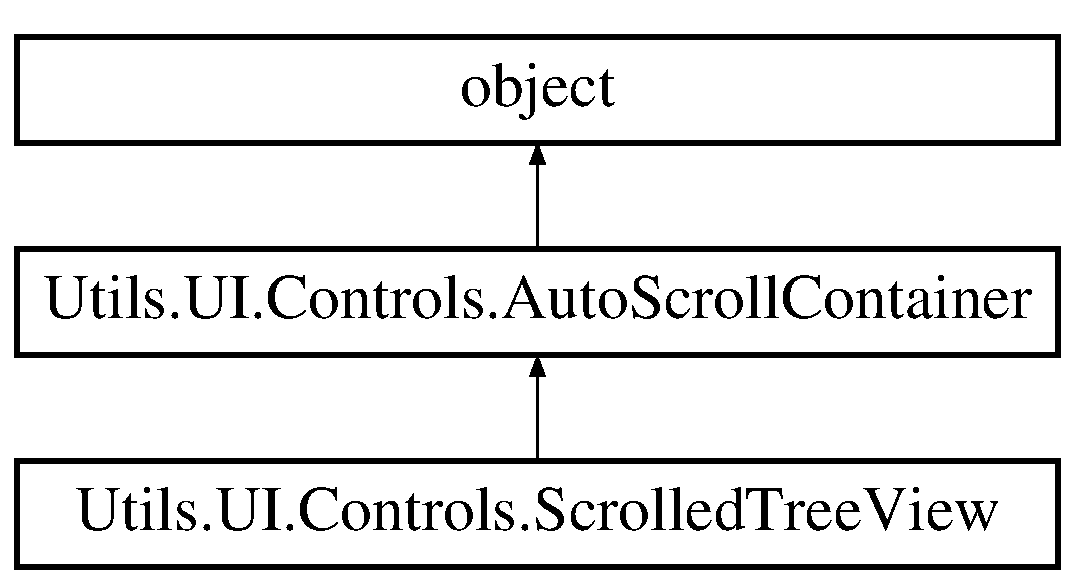
\includegraphics[height=3.000000cm]{class_c_utils_1_1_utils_1_1_u_i_1_1_controls_1_1_auto_scroll_container}
\end{center}
\end{figure}
\subsection*{Public Member Functions}
\begin{DoxyCompactItemize}
\item 
\mbox{\Hypertarget{class_c_utils_1_1_utils_1_1_u_i_1_1_controls_1_1_auto_scroll_container_aa7a4e2c13d6198a41bbf8f878589394b}\label{class_c_utils_1_1_utils_1_1_u_i_1_1_controls_1_1_auto_scroll_container_aa7a4e2c13d6198a41bbf8f878589394b}} 
def {\bfseries \+\_\+\+\_\+init\+\_\+\+\_\+} (self, master)
\end{DoxyCompactItemize}
\subsection*{Static Public Member Functions}
\begin{DoxyCompactItemize}
\item 
def \hyperlink{class_c_utils_1_1_utils_1_1_u_i_1_1_controls_1_1_auto_scroll_container_a94fb94a578671e4db721caa0034bee9a}{On\+Autoscroll} (scrollbar)
\end{DoxyCompactItemize}


\subsection{Detailed Description}


Definition at line 737 of file C\+Utils.\+py.



\subsection{Member Function Documentation}
\mbox{\Hypertarget{class_c_utils_1_1_utils_1_1_u_i_1_1_controls_1_1_auto_scroll_container_a94fb94a578671e4db721caa0034bee9a}\label{class_c_utils_1_1_utils_1_1_u_i_1_1_controls_1_1_auto_scroll_container_a94fb94a578671e4db721caa0034bee9a}} 
\index{C\+Utils\+::\+Utils\+::\+U\+I\+::\+Controls\+::\+Auto\+Scroll\+Container@{C\+Utils\+::\+Utils\+::\+U\+I\+::\+Controls\+::\+Auto\+Scroll\+Container}!On\+Autoscroll@{On\+Autoscroll}}
\index{On\+Autoscroll@{On\+Autoscroll}!C\+Utils\+::\+Utils\+::\+U\+I\+::\+Controls\+::\+Auto\+Scroll\+Container@{C\+Utils\+::\+Utils\+::\+U\+I\+::\+Controls\+::\+Auto\+Scroll\+Container}}
\subsubsection{\texorpdfstring{On\+Autoscroll()}{OnAutoscroll()}}
{\footnotesize\ttfamily def On\+Autoscroll (\begin{DoxyParamCaption}\item[{}]{scrollbar }\end{DoxyParamCaption})\hspace{0.3cm}{\ttfamily [static]}}

\begin{DoxyVerb}Hide and show scrollbar as needed.\end{DoxyVerb}
 

Definition at line 772 of file C\+Utils.\+py.



The documentation for this class was generated from the following file\+:\begin{DoxyCompactItemize}
\item 
C\+Utils.\+py\end{DoxyCompactItemize}

\hypertarget{class_c_simulation_1_1_simulation_1_1_building}{}\section{Simulation.\+Building Class Reference}
\label{class_c_simulation_1_1_simulation_1_1_building}\index{Simulation.\+Building@{Simulation.\+Building}}
Inheritance diagram for Simulation.\+Building\+:\begin{figure}[H]
\begin{center}
\leavevmode
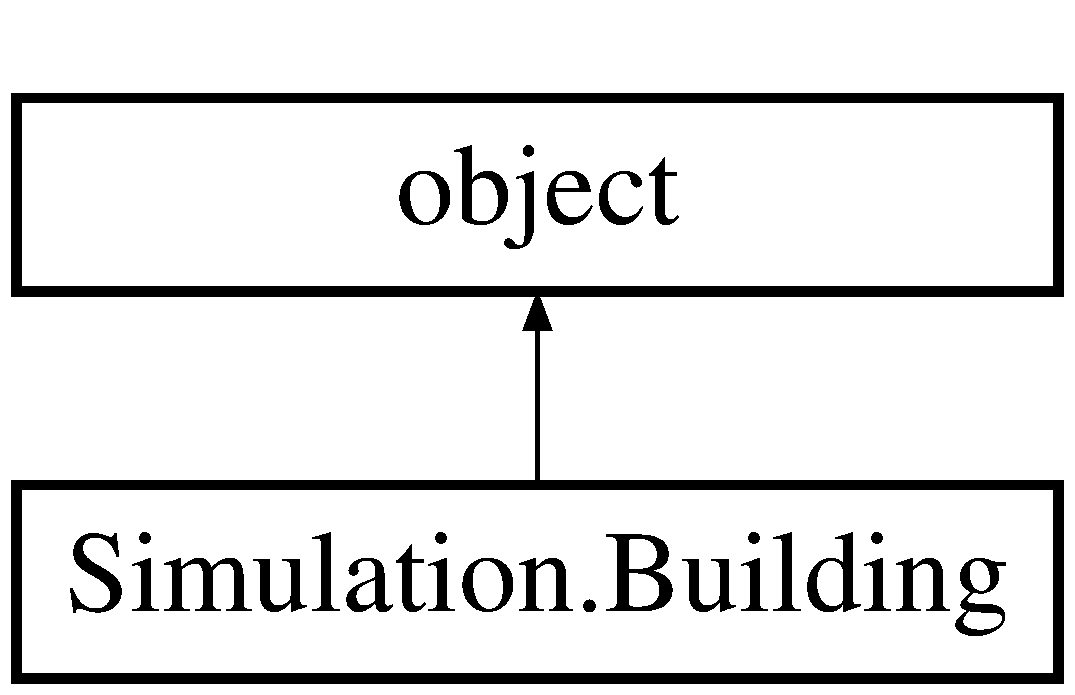
\includegraphics[height=2.000000cm]{class_c_simulation_1_1_simulation_1_1_building}
\end{center}
\end{figure}
\subsection*{Classes}
\begin{DoxyCompactItemize}
\item 
class \hyperlink{class_c_simulation_1_1_simulation_1_1_building_1_1_occupant}{Occupant}
\item 
class \hyperlink{class_c_simulation_1_1_simulation_1_1_building_1_1_zone}{Zone}
\end{DoxyCompactItemize}
\subsection*{Public Member Functions}
\begin{DoxyCompactItemize}
\item 
\mbox{\Hypertarget{class_c_simulation_1_1_simulation_1_1_building_a005f8f2d5acfee7d24d1aac6005a1e0a}\label{class_c_simulation_1_1_simulation_1_1_building_a005f8f2d5acfee7d24d1aac6005a1e0a}} 
def {\bfseries get\+Key} (self)
\item 
\mbox{\Hypertarget{class_c_simulation_1_1_simulation_1_1_building_a0c6ebeeeab67ba9a1868291123bc484f}\label{class_c_simulation_1_1_simulation_1_1_building_a0c6ebeeeab67ba9a1868291123bc484f}} 
def {\bfseries clear\+Zones} (self)
\item 
\mbox{\Hypertarget{class_c_simulation_1_1_simulation_1_1_building_a0cddba616803a5265a0c765be092ed95}\label{class_c_simulation_1_1_simulation_1_1_building_a0cddba616803a5265a0c765be092ed95}} 
def {\bfseries clear\+Occupants} (self)
\item 
\mbox{\Hypertarget{class_c_simulation_1_1_simulation_1_1_building_ab6b246e5565eb24f051005f6f483bc2a}\label{class_c_simulation_1_1_simulation_1_1_building_ab6b246e5565eb24f051005f6f483bc2a}} 
def {\bfseries get\+Zone\+By\+Name} (self, zone\+Name)
\item 
\mbox{\Hypertarget{class_c_simulation_1_1_simulation_1_1_building_af7078bbb194f02b25eda963059d3a896}\label{class_c_simulation_1_1_simulation_1_1_building_af7078bbb194f02b25eda963059d3a896}} 
def {\bfseries \+\_\+\+\_\+init\+\_\+\+\_\+} (self, id=0, name=\char`\"{}\char`\"{}, zones=None, occupants=None)
\item 
\mbox{\Hypertarget{class_c_simulation_1_1_simulation_1_1_building_a9a47563093dfc5ba12274b66e368920c}\label{class_c_simulation_1_1_simulation_1_1_building_a9a47563093dfc5ba12274b66e368920c}} 
def {\bfseries \+\_\+\+\_\+repr\+\_\+\+\_\+} (self)
\item 
\mbox{\Hypertarget{class_c_simulation_1_1_simulation_1_1_building_a157f9a5d3230b5fbbcb1391575ca1662}\label{class_c_simulation_1_1_simulation_1_1_building_a157f9a5d3230b5fbbcb1391575ca1662}} 
def {\bfseries \+\_\+\+\_\+cmp\+\_\+\+\_\+} (self, other)
\end{DoxyCompactItemize}
\subsection*{Public Attributes}
\begin{DoxyCompactItemize}
\item 
\mbox{\Hypertarget{class_c_simulation_1_1_simulation_1_1_building_acf2488b95c97e0378c9bf49de3b50f28}\label{class_c_simulation_1_1_simulation_1_1_building_acf2488b95c97e0378c9bf49de3b50f28}} 
{\bfseries id}
\item 
\mbox{\Hypertarget{class_c_simulation_1_1_simulation_1_1_building_ab74e6bf80237ddc4109968cedc58c151}\label{class_c_simulation_1_1_simulation_1_1_building_ab74e6bf80237ddc4109968cedc58c151}} 
{\bfseries name}
\item 
\mbox{\Hypertarget{class_c_simulation_1_1_simulation_1_1_building_a5470eb43ca93def6f1c6c1241e08fb38}\label{class_c_simulation_1_1_simulation_1_1_building_a5470eb43ca93def6f1c6c1241e08fb38}} 
{\bfseries zones}
\item 
\mbox{\Hypertarget{class_c_simulation_1_1_simulation_1_1_building_a6bcc1aeccf6379863ed9aad40a45505c}\label{class_c_simulation_1_1_simulation_1_1_building_a6bcc1aeccf6379863ed9aad40a45505c}} 
{\bfseries occupants}
\end{DoxyCompactItemize}


\subsection{Detailed Description}


Definition at line 17 of file C\+Simulation.\+py.



The documentation for this class was generated from the following file\+:\begin{DoxyCompactItemize}
\item 
C\+Simulation.\+py\end{DoxyCompactItemize}

\hypertarget{class_c_utils_1_1_utils_1_1_u_i_1_1_controls_1_1_cascading_drop_down_list}{}\section{Utils.\+U\+I.\+Controls.\+Cascading\+Drop\+Down\+List Class Reference}
\label{class_c_utils_1_1_utils_1_1_u_i_1_1_controls_1_1_cascading_drop_down_list}\index{Utils.\+U\+I.\+Controls.\+Cascading\+Drop\+Down\+List@{Utils.\+U\+I.\+Controls.\+Cascading\+Drop\+Down\+List}}
Inheritance diagram for Utils.\+U\+I.\+Controls.\+Cascading\+Drop\+Down\+List\+:\begin{figure}[H]
\begin{center}
\leavevmode
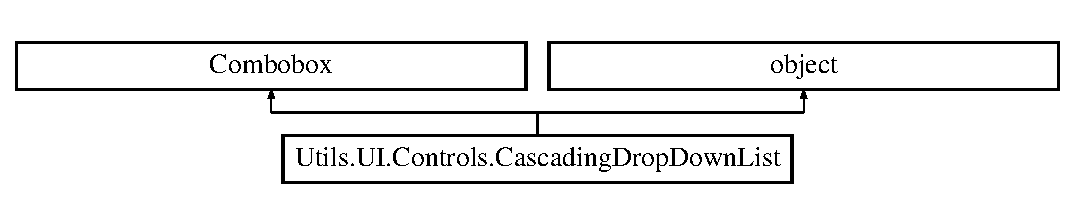
\includegraphics[height=2.000000cm]{class_c_utils_1_1_utils_1_1_u_i_1_1_controls_1_1_cascading_drop_down_list}
\end{center}
\end{figure}
\subsection*{Public Member Functions}
\begin{DoxyCompactItemize}
\item 
\mbox{\Hypertarget{class_c_utils_1_1_utils_1_1_u_i_1_1_controls_1_1_cascading_drop_down_list_a90eb243f26a86bc38d244f3739903784}\label{class_c_utils_1_1_utils_1_1_u_i_1_1_controls_1_1_cascading_drop_down_list_a90eb243f26a86bc38d244f3739903784}} 
def {\bfseries update\+List} (self)
\item 
\mbox{\Hypertarget{class_c_utils_1_1_utils_1_1_u_i_1_1_controls_1_1_cascading_drop_down_list_acbb5ee6f0b020063313ad70ad4b6e38f}\label{class_c_utils_1_1_utils_1_1_u_i_1_1_controls_1_1_cascading_drop_down_list_acbb5ee6f0b020063313ad70ad4b6e38f}} 
def {\bfseries set\+Value} (self, value)
\item 
\mbox{\Hypertarget{class_c_utils_1_1_utils_1_1_u_i_1_1_controls_1_1_cascading_drop_down_list_a6461a5bc77ce2c6d5c6b25fc3abaccc1}\label{class_c_utils_1_1_utils_1_1_u_i_1_1_controls_1_1_cascading_drop_down_list_a6461a5bc77ce2c6d5c6b25fc3abaccc1}} 
def {\bfseries On\+Selection\+Event} (self, event)
\item 
\mbox{\Hypertarget{class_c_utils_1_1_utils_1_1_u_i_1_1_controls_1_1_cascading_drop_down_list_a2d9f1b9bed847ff75b9f232ced637286}\label{class_c_utils_1_1_utils_1_1_u_i_1_1_controls_1_1_cascading_drop_down_list_a2d9f1b9bed847ff75b9f232ced637286}} 
def {\bfseries \+\_\+\+\_\+init\+\_\+\+\_\+} (self, parent, args, kwargs)
\end{DoxyCompactItemize}


\subsection{Detailed Description}


Definition at line 467 of file C\+Utils.\+py.



The documentation for this class was generated from the following file\+:\begin{DoxyCompactItemize}
\item 
C\+Utils.\+py\end{DoxyCompactItemize}

\hypertarget{class_c_building_1_1_c_building}{}\section{C\+Building Class Reference}
\label{class_c_building_1_1_c_building}\index{C\+Building@{C\+Building}}
Inheritance diagram for C\+Building\+:\begin{figure}[H]
\begin{center}
\leavevmode
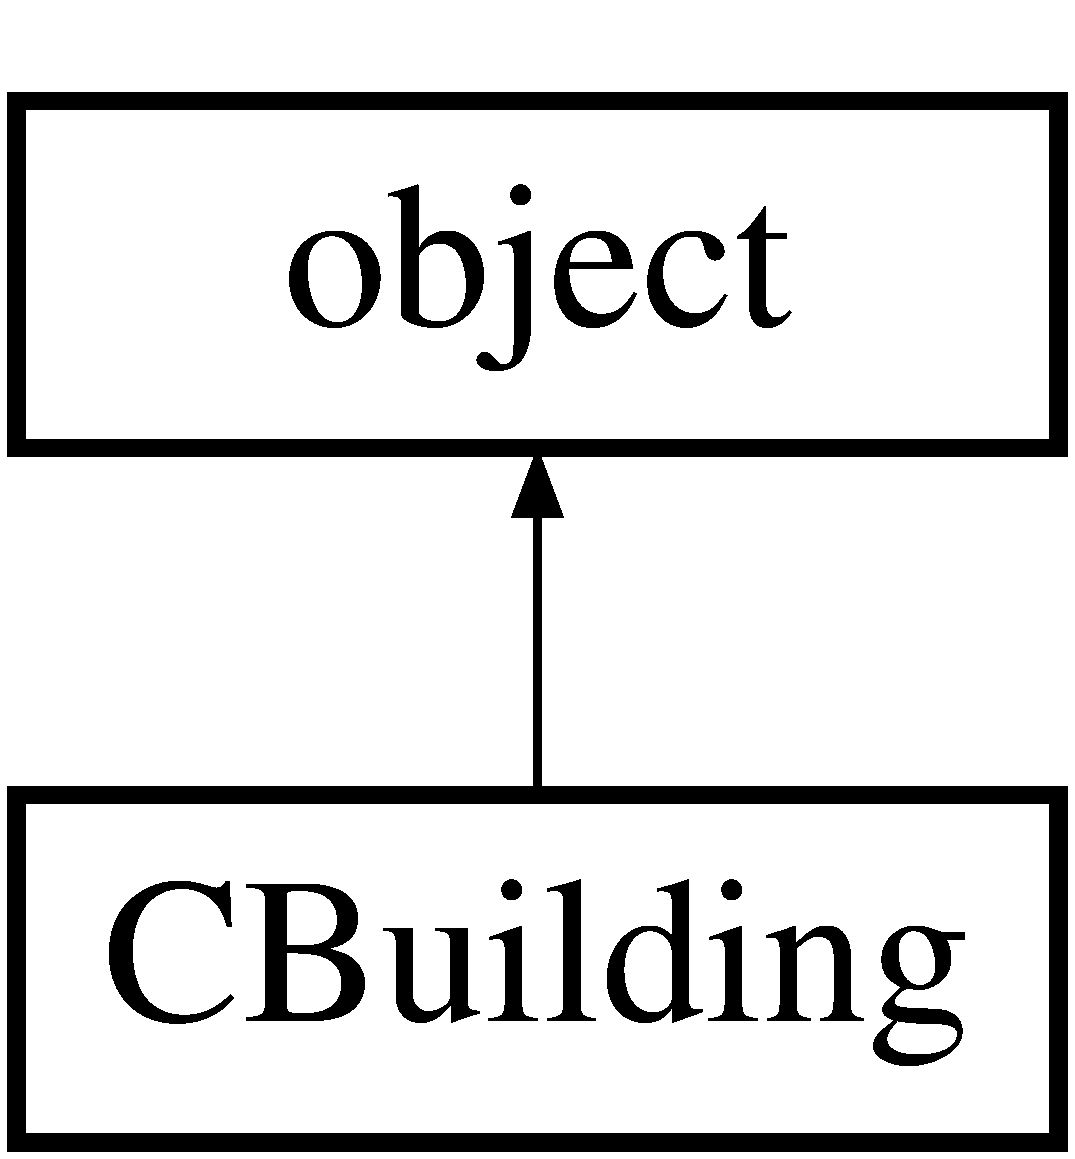
\includegraphics[height=2.000000cm]{class_c_building_1_1_c_building}
\end{center}
\end{figure}
\subsection*{Public Member Functions}
\begin{DoxyCompactItemize}
\item 
\mbox{\Hypertarget{class_c_building_1_1_c_building_abbcfc1a774079da020e49c42cbadb693}\label{class_c_building_1_1_c_building_abbcfc1a774079da020e49c42cbadb693}} 
def {\bfseries U\+U\+ID} (self)
\item 
\mbox{\Hypertarget{class_c_building_1_1_c_building_aff464267544e4efc9b770c8320c8f199}\label{class_c_building_1_1_c_building_aff464267544e4efc9b770c8320c8f199}} 
def {\bfseries type} (self)
\item 
\mbox{\Hypertarget{class_c_building_1_1_c_building_aca033702f187894894d3102de41d6b99}\label{class_c_building_1_1_c_building_aca033702f187894894d3102de41d6b99}} 
def {\bfseries type} (self, value)
\item 
\mbox{\Hypertarget{class_c_building_1_1_c_building_adb8818239148d2e5c5833a2b062ee9ad}\label{class_c_building_1_1_c_building_adb8818239148d2e5c5833a2b062ee9ad}} 
def {\bfseries ID} (self)
\item 
\mbox{\Hypertarget{class_c_building_1_1_c_building_a0a178fbcae3f6431733dd63ee37ac7bb}\label{class_c_building_1_1_c_building_a0a178fbcae3f6431733dd63ee37ac7bb}} 
def {\bfseries ID} (self, value)
\item 
\mbox{\Hypertarget{class_c_building_1_1_c_building_a5907ca3bbf8e7cd8f40c3007338f6d02}\label{class_c_building_1_1_c_building_a5907ca3bbf8e7cd8f40c3007338f6d02}} 
def {\bfseries name} (self)
\item 
\mbox{\Hypertarget{class_c_building_1_1_c_building_a62d212fdcbbcee30e90a64ce349d32f8}\label{class_c_building_1_1_c_building_a62d212fdcbbcee30e90a64ce349d32f8}} 
def {\bfseries name} (self, value)
\item 
\mbox{\Hypertarget{class_c_building_1_1_c_building_aaf00860c69345f71509aa2520eb5bfa7}\label{class_c_building_1_1_c_building_aaf00860c69345f71509aa2520eb5bfa7}} 
def {\bfseries \+\_\+\+\_\+init\+\_\+\+\_\+} (self, id=0, name=\textquotesingle{}\textquotesingle{})
\end{DoxyCompactItemize}


\subsection{Detailed Description}


Definition at line 12 of file C\+Building.\+py.



The documentation for this class was generated from the following file\+:\begin{DoxyCompactItemize}
\item 
C\+Building.\+py\end{DoxyCompactItemize}

\hypertarget{class_c_lights_1_1_c_lights}{}\section{C\+Lights Class Reference}
\label{class_c_lights_1_1_c_lights}\index{C\+Lights@{C\+Lights}}
Inheritance diagram for C\+Lights\+:\begin{figure}[H]
\begin{center}
\leavevmode
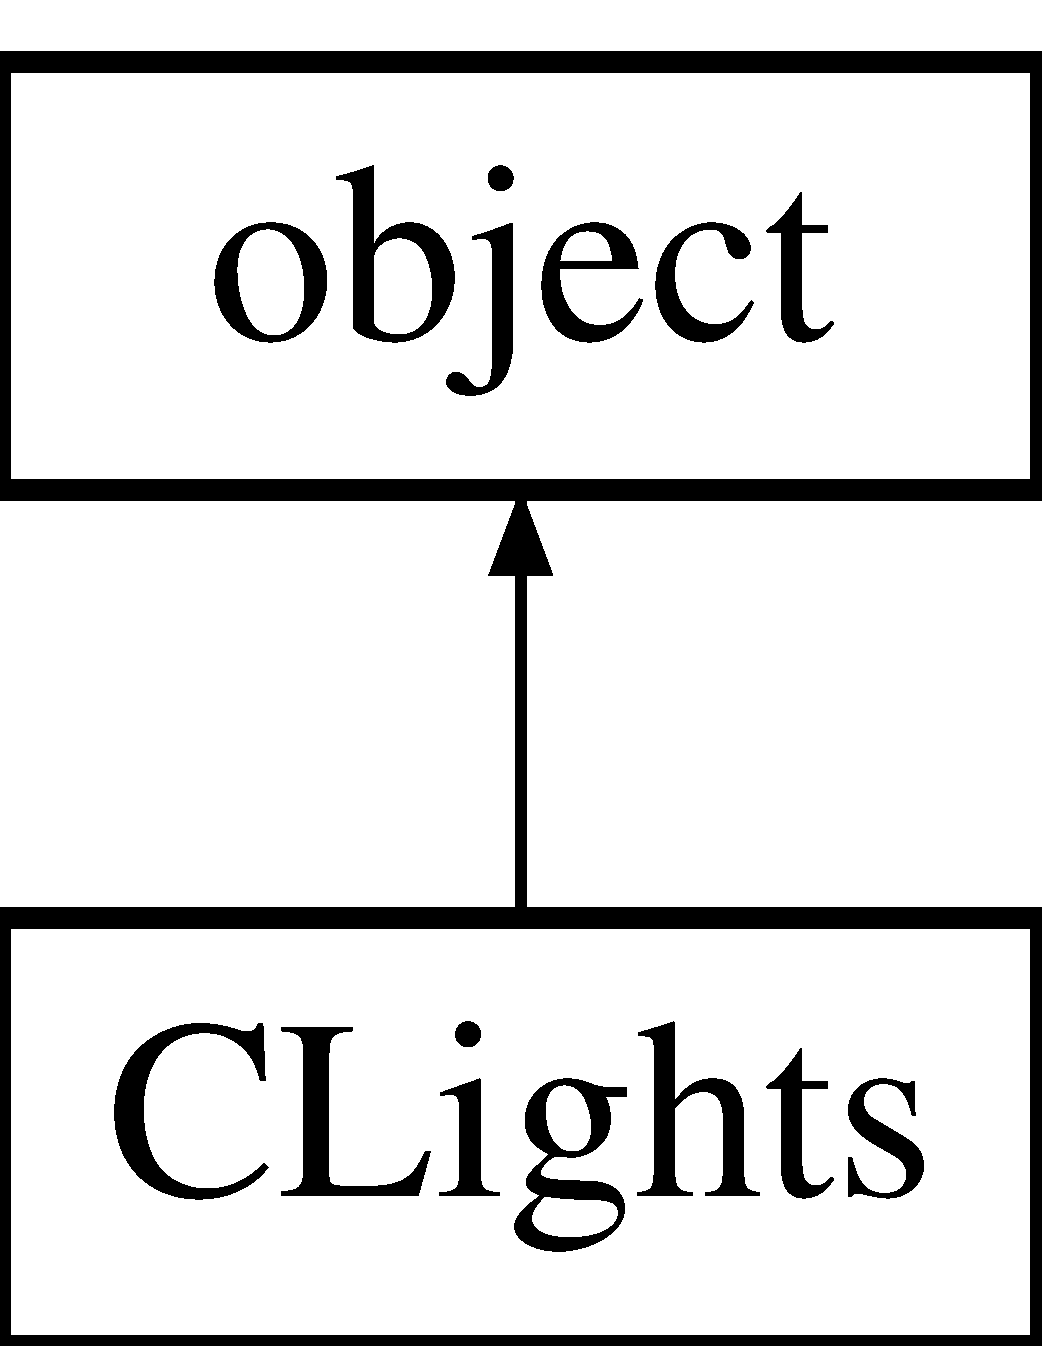
\includegraphics[height=2.000000cm]{class_c_lights_1_1_c_lights}
\end{center}
\end{figure}
\subsection*{Public Member Functions}
\begin{DoxyCompactItemize}
\item 
\mbox{\Hypertarget{class_c_lights_1_1_c_lights_abbcfc1a774079da020e49c42cbadb693}\label{class_c_lights_1_1_c_lights_abbcfc1a774079da020e49c42cbadb693}} 
def {\bfseries U\+U\+ID} (self)
\item 
\mbox{\Hypertarget{class_c_lights_1_1_c_lights_aff464267544e4efc9b770c8320c8f199}\label{class_c_lights_1_1_c_lights_aff464267544e4efc9b770c8320c8f199}} 
def {\bfseries type} (self)
\item 
\mbox{\Hypertarget{class_c_lights_1_1_c_lights_aca033702f187894894d3102de41d6b99}\label{class_c_lights_1_1_c_lights_aca033702f187894894d3102de41d6b99}} 
def {\bfseries type} (self, value)
\item 
\mbox{\Hypertarget{class_c_lights_1_1_c_lights_adb8818239148d2e5c5833a2b062ee9ad}\label{class_c_lights_1_1_c_lights_adb8818239148d2e5c5833a2b062ee9ad}} 
def {\bfseries ID} (self)
\item 
\mbox{\Hypertarget{class_c_lights_1_1_c_lights_a0a178fbcae3f6431733dd63ee37ac7bb}\label{class_c_lights_1_1_c_lights_a0a178fbcae3f6431733dd63ee37ac7bb}} 
def {\bfseries ID} (self, value)
\item 
\mbox{\Hypertarget{class_c_lights_1_1_c_lights_a05cd4cd28b324f262fefe1a1782bd992}\label{class_c_lights_1_1_c_lights_a05cd4cd28b324f262fefe1a1782bd992}} 
def {\bfseries enabled} (self)
\item 
\mbox{\Hypertarget{class_c_lights_1_1_c_lights_a18495e0c3f2639c84751c9aa77cd03b3}\label{class_c_lights_1_1_c_lights_a18495e0c3f2639c84751c9aa77cd03b3}} 
def {\bfseries enabled} (self, value)
\item 
\mbox{\Hypertarget{class_c_lights_1_1_c_lights_a71963b9940a29bf3f2c10546c2cb9b50}\label{class_c_lights_1_1_c_lights_a71963b9940a29bf3f2c10546c2cb9b50}} 
def {\bfseries \+\_\+\+\_\+init\+\_\+\+\_\+} (self, id=str(uuid.\+uuid4()), enabled=True)
\end{DoxyCompactItemize}


\subsection{Detailed Description}


Definition at line 12 of file C\+Lights.\+py.



The documentation for this class was generated from the following file\+:\begin{DoxyCompactItemize}
\item 
C\+Lights.\+py\end{DoxyCompactItemize}

\hypertarget{class_c_occupant_1_1_c_occupant}{}\section{C\+Occupant Class Reference}
\label{class_c_occupant_1_1_c_occupant}\index{C\+Occupant@{C\+Occupant}}
Inheritance diagram for C\+Occupant\+:\begin{figure}[H]
\begin{center}
\leavevmode
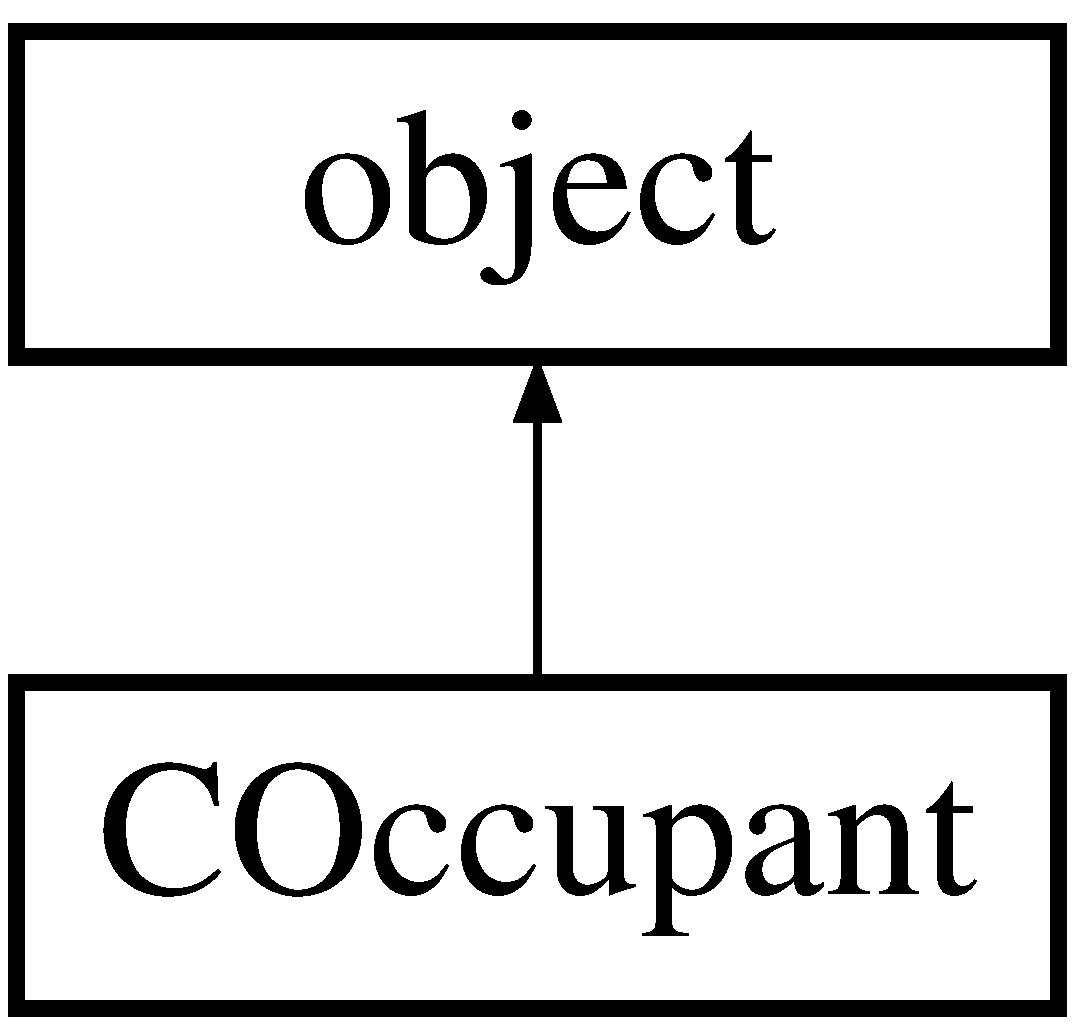
\includegraphics[height=2.000000cm]{class_c_occupant_1_1_c_occupant}
\end{center}
\end{figure}
\subsection*{Public Member Functions}
\begin{DoxyCompactItemize}
\item 
\mbox{\Hypertarget{class_c_occupant_1_1_c_occupant_abbcfc1a774079da020e49c42cbadb693}\label{class_c_occupant_1_1_c_occupant_abbcfc1a774079da020e49c42cbadb693}} 
def {\bfseries U\+U\+ID} (self)
\item 
\mbox{\Hypertarget{class_c_occupant_1_1_c_occupant_aff464267544e4efc9b770c8320c8f199}\label{class_c_occupant_1_1_c_occupant_aff464267544e4efc9b770c8320c8f199}} 
def {\bfseries type} (self)
\item 
\mbox{\Hypertarget{class_c_occupant_1_1_c_occupant_aca033702f187894894d3102de41d6b99}\label{class_c_occupant_1_1_c_occupant_aca033702f187894894d3102de41d6b99}} 
def {\bfseries type} (self, value)
\item 
\mbox{\Hypertarget{class_c_occupant_1_1_c_occupant_adb8818239148d2e5c5833a2b062ee9ad}\label{class_c_occupant_1_1_c_occupant_adb8818239148d2e5c5833a2b062ee9ad}} 
def {\bfseries ID} (self)
\item 
\mbox{\Hypertarget{class_c_occupant_1_1_c_occupant_a0a178fbcae3f6431733dd63ee37ac7bb}\label{class_c_occupant_1_1_c_occupant_a0a178fbcae3f6431733dd63ee37ac7bb}} 
def {\bfseries ID} (self, value)
\item 
\mbox{\Hypertarget{class_c_occupant_1_1_c_occupant_a5907ca3bbf8e7cd8f40c3007338f6d02}\label{class_c_occupant_1_1_c_occupant_a5907ca3bbf8e7cd8f40c3007338f6d02}} 
def {\bfseries name} (self)
\item 
\mbox{\Hypertarget{class_c_occupant_1_1_c_occupant_a62d212fdcbbcee30e90a64ce349d32f8}\label{class_c_occupant_1_1_c_occupant_a62d212fdcbbcee30e90a64ce349d32f8}} 
def {\bfseries name} (self, value)
\item 
\mbox{\Hypertarget{class_c_occupant_1_1_c_occupant_a8f87fa90d837591b33eb32ed88428676}\label{class_c_occupant_1_1_c_occupant_a8f87fa90d837591b33eb32ed88428676}} 
def {\bfseries zone\+Id} (self)
\item 
\mbox{\Hypertarget{class_c_occupant_1_1_c_occupant_affc3fc983b593a33c7f975022f77eece}\label{class_c_occupant_1_1_c_occupant_affc3fc983b593a33c7f975022f77eece}} 
def {\bfseries zone\+Id} (self, value)
\item 
\mbox{\Hypertarget{class_c_occupant_1_1_c_occupant_a5c56d4145461f904b35e53e48b74f119}\label{class_c_occupant_1_1_c_occupant_a5c56d4145461f904b35e53e48b74f119}} 
def {\bfseries zone} (self)
\item 
\mbox{\Hypertarget{class_c_occupant_1_1_c_occupant_a26d49d39f5f1dbcdb4107000a31e2deb}\label{class_c_occupant_1_1_c_occupant_a26d49d39f5f1dbcdb4107000a31e2deb}} 
def {\bfseries zone} (self, value)
\item 
\mbox{\Hypertarget{class_c_occupant_1_1_c_occupant_ae1f27c9c7a3592383d4e68225d3951a3}\label{class_c_occupant_1_1_c_occupant_ae1f27c9c7a3592383d4e68225d3951a3}} 
def {\bfseries power} (self)
\item 
\mbox{\Hypertarget{class_c_occupant_1_1_c_occupant_ab3385809bc06f15b487dc5af6df7bfe9}\label{class_c_occupant_1_1_c_occupant_ab3385809bc06f15b487dc5af6df7bfe9}} 
def {\bfseries power} (self, value)
\item 
\mbox{\Hypertarget{class_c_occupant_1_1_c_occupant_aa48dde3f738de560f586688797945169}\label{class_c_occupant_1_1_c_occupant_aa48dde3f738de560f586688797945169}} 
def {\bfseries window\+Id} (self)
\item 
\mbox{\Hypertarget{class_c_occupant_1_1_c_occupant_ab13145f4656f2db6383e6e01e0017dd0}\label{class_c_occupant_1_1_c_occupant_ab13145f4656f2db6383e6e01e0017dd0}} 
def {\bfseries window\+Id} (self, value)
\item 
\mbox{\Hypertarget{class_c_occupant_1_1_c_occupant_aebb1c45619dc8d4d15fa40bf872ed1b6}\label{class_c_occupant_1_1_c_occupant_aebb1c45619dc8d4d15fa40bf872ed1b6}} 
def {\bfseries window} (self)
\item 
\mbox{\Hypertarget{class_c_occupant_1_1_c_occupant_a25ba82e247aab3d2e0fc5be936eee197}\label{class_c_occupant_1_1_c_occupant_a25ba82e247aab3d2e0fc5be936eee197}} 
def {\bfseries window} (self, value)
\item 
\mbox{\Hypertarget{class_c_occupant_1_1_c_occupant_affa1d82b874a94f155f908d34648ab73}\label{class_c_occupant_1_1_c_occupant_affa1d82b874a94f155f908d34648ab73}} 
def {\bfseries shade\+Id} (self)
\item 
\mbox{\Hypertarget{class_c_occupant_1_1_c_occupant_ae95ef2a337b6d53e911e700b87d722f7}\label{class_c_occupant_1_1_c_occupant_ae95ef2a337b6d53e911e700b87d722f7}} 
def {\bfseries shade\+Id} (self, value)
\item 
\mbox{\Hypertarget{class_c_occupant_1_1_c_occupant_a2f2f39f18d932f6db92cb0df5aca42b8}\label{class_c_occupant_1_1_c_occupant_a2f2f39f18d932f6db92cb0df5aca42b8}} 
def {\bfseries shade} (self)
\item 
\mbox{\Hypertarget{class_c_occupant_1_1_c_occupant_a2248be7e908a5882b293136431c70883}\label{class_c_occupant_1_1_c_occupant_a2248be7e908a5882b293136431c70883}} 
def {\bfseries shade} (self, value)
\item 
\mbox{\Hypertarget{class_c_occupant_1_1_c_occupant_a358a404bcbb9bc67ab0eb6fbd49a5b25}\label{class_c_occupant_1_1_c_occupant_a358a404bcbb9bc67ab0eb6fbd49a5b25}} 
def {\bfseries activity\+Id} (self)
\item 
\mbox{\Hypertarget{class_c_occupant_1_1_c_occupant_adc8581be09aff51f2cc4cfdd66f6a509}\label{class_c_occupant_1_1_c_occupant_adc8581be09aff51f2cc4cfdd66f6a509}} 
def {\bfseries activity\+Id} (self, value)
\item 
\mbox{\Hypertarget{class_c_occupant_1_1_c_occupant_ac9916df25ee63c151e00c568bae60717}\label{class_c_occupant_1_1_c_occupant_ac9916df25ee63c151e00c568bae60717}} 
def {\bfseries sex} (self)
\item 
\mbox{\Hypertarget{class_c_occupant_1_1_c_occupant_afe7bc08b2b77f3852de9baa5fe21d62e}\label{class_c_occupant_1_1_c_occupant_afe7bc08b2b77f3852de9baa5fe21d62e}} 
def {\bfseries sex} (self, value)
\item 
\mbox{\Hypertarget{class_c_occupant_1_1_c_occupant_ae52f20c05f9dc68a818119de5cac4959}\label{class_c_occupant_1_1_c_occupant_ae52f20c05f9dc68a818119de5cac4959}} 
def {\bfseries family\+ID} (self)
\item 
\mbox{\Hypertarget{class_c_occupant_1_1_c_occupant_aed2f2289f06af1cca08da867cf895b1e}\label{class_c_occupant_1_1_c_occupant_aed2f2289f06af1cca08da867cf895b1e}} 
def {\bfseries family\+ID} (self, value)
\item 
\mbox{\Hypertarget{class_c_occupant_1_1_c_occupant_a4e2fe095db97dc3824f02c14a52dd392}\label{class_c_occupant_1_1_c_occupant_a4e2fe095db97dc3824f02c14a52dd392}} 
def {\bfseries education\+ID} (self)
\item 
\mbox{\Hypertarget{class_c_occupant_1_1_c_occupant_af022ef50417facda91670c62bb6f4df3}\label{class_c_occupant_1_1_c_occupant_af022ef50417facda91670c62bb6f4df3}} 
def {\bfseries education\+ID} (self, value)
\item 
\mbox{\Hypertarget{class_c_occupant_1_1_c_occupant_a096592926573dc4b0035536e0dc1bcaa}\label{class_c_occupant_1_1_c_occupant_a096592926573dc4b0035536e0dc1bcaa}} 
def {\bfseries age\+Group} (self)
\item 
\mbox{\Hypertarget{class_c_occupant_1_1_c_occupant_a489e43626268c1631a16ab1870428028}\label{class_c_occupant_1_1_c_occupant_a489e43626268c1631a16ab1870428028}} 
def {\bfseries age\+Group} (self, value)
\item 
\mbox{\Hypertarget{class_c_occupant_1_1_c_occupant_a7fc057b39b04027270b799ca1c138ebf}\label{class_c_occupant_1_1_c_occupant_a7fc057b39b04027270b799ca1c138ebf}} 
def {\bfseries own\+Computer} (self)
\item 
\mbox{\Hypertarget{class_c_occupant_1_1_c_occupant_ab974a46cc60baeb212aa812602fa2eed}\label{class_c_occupant_1_1_c_occupant_ab974a46cc60baeb212aa812602fa2eed}} 
def {\bfseries own\+Computer} (self, value)
\item 
\mbox{\Hypertarget{class_c_occupant_1_1_c_occupant_a7c7c5a0fc017c9ec665717842c4f4e67}\label{class_c_occupant_1_1_c_occupant_a7c7c5a0fc017c9ec665717842c4f4e67}} 
def {\bfseries is\+Retired} (self)
\item 
\mbox{\Hypertarget{class_c_occupant_1_1_c_occupant_a8b38f4f59dda44568dfeb4eb6961d8bd}\label{class_c_occupant_1_1_c_occupant_a8b38f4f59dda44568dfeb4eb6961d8bd}} 
def {\bfseries is\+Retired} (self, value)
\item 
\mbox{\Hypertarget{class_c_occupant_1_1_c_occupant_a78e6786872d42edd1f116cf002a88740}\label{class_c_occupant_1_1_c_occupant_a78e6786872d42edd1f116cf002a88740}} 
def {\bfseries is\+Married} (self)
\item 
\mbox{\Hypertarget{class_c_occupant_1_1_c_occupant_a79380d637b350ffdcdc6f72a8a28405b}\label{class_c_occupant_1_1_c_occupant_a79380d637b350ffdcdc6f72a8a28405b}} 
def {\bfseries is\+Married} (self, value)
\item 
\mbox{\Hypertarget{class_c_occupant_1_1_c_occupant_a1904b99f5ec8532431543db3bf3a644a}\label{class_c_occupant_1_1_c_occupant_a1904b99f5ec8532431543db3bf3a644a}} 
def {\bfseries is\+Un\+Employed} (self)
\item 
\mbox{\Hypertarget{class_c_occupant_1_1_c_occupant_a67b635cd2fcec6bba83c64e3fa3ca666}\label{class_c_occupant_1_1_c_occupant_a67b635cd2fcec6bba83c64e3fa3ca666}} 
def {\bfseries is\+Un\+Employed} (self, value)
\item 
\mbox{\Hypertarget{class_c_occupant_1_1_c_occupant_af5b9c2383c9368414aac2740c737d9d9}\label{class_c_occupant_1_1_c_occupant_af5b9c2383c9368414aac2740c737d9d9}} 
def {\bfseries \+\_\+\+\_\+init\+\_\+\+\_\+} (self, id=0, name=\textquotesingle{}\textquotesingle{}, zone\+Id=\textquotesingle{}\textquotesingle{}, zone=\textquotesingle{}\textquotesingle{}, power=0, window\+Id=\textquotesingle{}\textquotesingle{}, window=\textquotesingle{}\textquotesingle{}, shade\+Id=\textquotesingle{}\textquotesingle{}, shade=\textquotesingle{}\textquotesingle{}, activity\+Id=\textquotesingle{}\textquotesingle{}, sex=\textquotesingle{}\textquotesingle{}, family\+ID=\textquotesingle{}\textquotesingle{}, education\+ID=\textquotesingle{}\textquotesingle{}, age\+Group=\textquotesingle{}\textquotesingle{}, own\+Computer=False, is\+Retired=False, is\+Married=False, is\+Un\+Employed=False)
\end{DoxyCompactItemize}


\subsection{Detailed Description}


Definition at line 12 of file C\+Occupant.\+py.



The documentation for this class was generated from the following file\+:\begin{DoxyCompactItemize}
\item 
C\+Occupant.\+py\end{DoxyCompactItemize}

\hypertarget{class_c_occupant_template_1_1_c_occupant_template}{}\section{C\+Occupant\+Template Class Reference}
\label{class_c_occupant_template_1_1_c_occupant_template}\index{C\+Occupant\+Template@{C\+Occupant\+Template}}
Inheritance diagram for C\+Occupant\+Template\+:\begin{figure}[H]
\begin{center}
\leavevmode
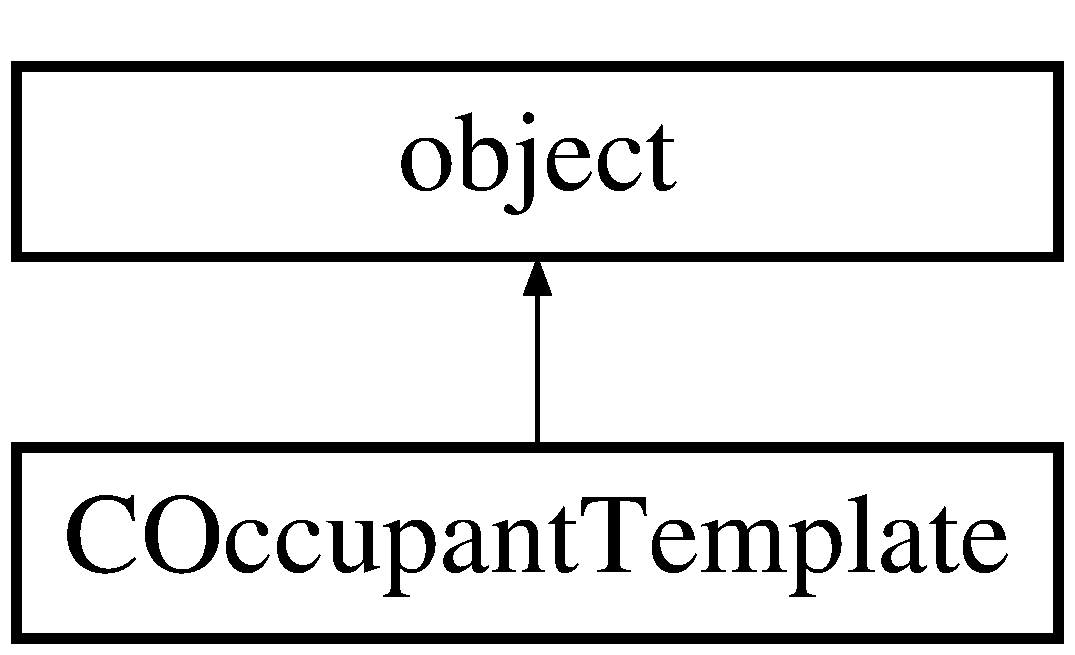
\includegraphics[height=2.000000cm]{class_c_occupant_template_1_1_c_occupant_template}
\end{center}
\end{figure}
\subsection*{Public Member Functions}
\begin{DoxyCompactItemize}
\item 
\mbox{\Hypertarget{class_c_occupant_template_1_1_c_occupant_template_abbcfc1a774079da020e49c42cbadb693}\label{class_c_occupant_template_1_1_c_occupant_template_abbcfc1a774079da020e49c42cbadb693}} 
def {\bfseries U\+U\+ID} (self)
\item 
\mbox{\Hypertarget{class_c_occupant_template_1_1_c_occupant_template_a17c9ca40c3df55189d0997a1662757cf}\label{class_c_occupant_template_1_1_c_occupant_template_a17c9ca40c3df55189d0997a1662757cf}} 
def {\bfseries U\+U\+ID} (self, value)
\item 
\mbox{\Hypertarget{class_c_occupant_template_1_1_c_occupant_template_aff464267544e4efc9b770c8320c8f199}\label{class_c_occupant_template_1_1_c_occupant_template_aff464267544e4efc9b770c8320c8f199}} 
def {\bfseries type} (self)
\item 
\mbox{\Hypertarget{class_c_occupant_template_1_1_c_occupant_template_aca033702f187894894d3102de41d6b99}\label{class_c_occupant_template_1_1_c_occupant_template_aca033702f187894894d3102de41d6b99}} 
def {\bfseries type} (self, value)
\item 
\mbox{\Hypertarget{class_c_occupant_template_1_1_c_occupant_template_adb8818239148d2e5c5833a2b062ee9ad}\label{class_c_occupant_template_1_1_c_occupant_template_adb8818239148d2e5c5833a2b062ee9ad}} 
def {\bfseries ID} (self)
\item 
\mbox{\Hypertarget{class_c_occupant_template_1_1_c_occupant_template_a0a178fbcae3f6431733dd63ee37ac7bb}\label{class_c_occupant_template_1_1_c_occupant_template_a0a178fbcae3f6431733dd63ee37ac7bb}} 
def {\bfseries ID} (self, value)
\item 
\mbox{\Hypertarget{class_c_occupant_template_1_1_c_occupant_template_a5907ca3bbf8e7cd8f40c3007338f6d02}\label{class_c_occupant_template_1_1_c_occupant_template_a5907ca3bbf8e7cd8f40c3007338f6d02}} 
def {\bfseries name} (self)
\item 
\mbox{\Hypertarget{class_c_occupant_template_1_1_c_occupant_template_a62d212fdcbbcee30e90a64ce349d32f8}\label{class_c_occupant_template_1_1_c_occupant_template_a62d212fdcbbcee30e90a64ce349d32f8}} 
def {\bfseries name} (self, value)
\item 
\mbox{\Hypertarget{class_c_occupant_template_1_1_c_occupant_template_a3690e5c2a8828abbe9153aeed1f5fecc}\label{class_c_occupant_template_1_1_c_occupant_template_a3690e5c2a8828abbe9153aeed1f5fecc}} 
def {\bfseries description} (self)
\item 
\mbox{\Hypertarget{class_c_occupant_template_1_1_c_occupant_template_a7653d8598140cb0974391375b6e0bf2d}\label{class_c_occupant_template_1_1_c_occupant_template_a7653d8598140cb0974391375b6e0bf2d}} 
def {\bfseries description} (self, value)
\item 
\mbox{\Hypertarget{class_c_occupant_template_1_1_c_occupant_template_af558b9f11e20d56424108300e3bafef5}\label{class_c_occupant_template_1_1_c_occupant_template_af558b9f11e20d56424108300e3bafef5}} 
def {\bfseries category\+ID} (self)
\item 
\mbox{\Hypertarget{class_c_occupant_template_1_1_c_occupant_template_adfa0996f4864e3307efcfa643cb7519c}\label{class_c_occupant_template_1_1_c_occupant_template_adfa0996f4864e3307efcfa643cb7519c}} 
def {\bfseries category\+ID} (self, value)
\item 
\mbox{\Hypertarget{class_c_occupant_template_1_1_c_occupant_template_a139e7e3973be16fd3cca7a132e7b4622}\label{class_c_occupant_template_1_1_c_occupant_template_a139e7e3973be16fd3cca7a132e7b4622}} 
def {\bfseries category} (self)
\item 
\mbox{\Hypertarget{class_c_occupant_template_1_1_c_occupant_template_ac685b03b444e0dd2089bb2d6da828b6d}\label{class_c_occupant_template_1_1_c_occupant_template_ac685b03b444e0dd2089bb2d6da828b6d}} 
def {\bfseries category} (self, value)
\item 
\mbox{\Hypertarget{class_c_occupant_template_1_1_c_occupant_template_a2d64382fb14878ff68fb76d8b5ac4d6b}\label{class_c_occupant_template_1_1_c_occupant_template_a2d64382fb14878ff68fb76d8b5ac4d6b}} 
def {\bfseries region\+ID} (self)
\item 
\mbox{\Hypertarget{class_c_occupant_template_1_1_c_occupant_template_a80ddda2986b04b9c6ad6581a70cb2d2c}\label{class_c_occupant_template_1_1_c_occupant_template_a80ddda2986b04b9c6ad6581a70cb2d2c}} 
def {\bfseries region\+ID} (self, value)
\item 
\mbox{\Hypertarget{class_c_occupant_template_1_1_c_occupant_template_ad1d284419b8527b6cdcdb0d544f12b7a}\label{class_c_occupant_template_1_1_c_occupant_template_ad1d284419b8527b6cdcdb0d544f12b7a}} 
def {\bfseries region} (self)
\item 
\mbox{\Hypertarget{class_c_occupant_template_1_1_c_occupant_template_a6bcc3de12f8bed0075e8e9fc8ee449bf}\label{class_c_occupant_template_1_1_c_occupant_template_a6bcc3de12f8bed0075e8e9fc8ee449bf}} 
def {\bfseries region} (self, value)
\item 
\mbox{\Hypertarget{class_c_occupant_template_1_1_c_occupant_template_a845d68804272d678014ec19ae4ec2bd4}\label{class_c_occupant_template_1_1_c_occupant_template_a845d68804272d678014ec19ae4ec2bd4}} 
def {\bfseries sector\+ID} (self)
\item 
\mbox{\Hypertarget{class_c_occupant_template_1_1_c_occupant_template_a39c05e74743100180589496adc2bc7f4}\label{class_c_occupant_template_1_1_c_occupant_template_a39c05e74743100180589496adc2bc7f4}} 
def {\bfseries sector\+ID} (self, value)
\item 
\mbox{\Hypertarget{class_c_occupant_template_1_1_c_occupant_template_ad87f4eda7b65f91e62a4fcaf83dd2a66}\label{class_c_occupant_template_1_1_c_occupant_template_ad87f4eda7b65f91e62a4fcaf83dd2a66}} 
def {\bfseries sector} (self)
\item 
\mbox{\Hypertarget{class_c_occupant_template_1_1_c_occupant_template_a10757cf61e95d007399167376cc5c46d}\label{class_c_occupant_template_1_1_c_occupant_template_a10757cf61e95d007399167376cc5c46d}} 
def {\bfseries sector} (self, value)
\item 
\mbox{\Hypertarget{class_c_occupant_template_1_1_c_occupant_template_acc81b7a03d171885bcca403afe3e4bae}\label{class_c_occupant_template_1_1_c_occupant_template_acc81b7a03d171885bcca403afe3e4bae}} 
def {\bfseries occupants} (self)
\item 
\mbox{\Hypertarget{class_c_occupant_template_1_1_c_occupant_template_a401fc8bbb2852e9f2bfadad6c6b81a92}\label{class_c_occupant_template_1_1_c_occupant_template_a401fc8bbb2852e9f2bfadad6c6b81a92}} 
def {\bfseries occupants} (self, array)
\item 
\mbox{\Hypertarget{class_c_occupant_template_1_1_c_occupant_template_a0b6512b01e0b9f391bd9fdb046f3df0a}\label{class_c_occupant_template_1_1_c_occupant_template_a0b6512b01e0b9f391bd9fdb046f3df0a}} 
def {\bfseries \+\_\+\+\_\+init\+\_\+\+\_\+} (self, id=0, name=\textquotesingle{}\textquotesingle{}, description=\textquotesingle{}\textquotesingle{}, category\+ID=\textquotesingle{}\textquotesingle{}, category=\textquotesingle{}\textquotesingle{}, region\+ID=\textquotesingle{}\textquotesingle{}, region=\textquotesingle{}\textquotesingle{}, sector\+ID=\textquotesingle{}\textquotesingle{}, sector=\textquotesingle{}\textquotesingle{}, occupants=None)
\end{DoxyCompactItemize}


\subsection{Detailed Description}


Definition at line 12 of file C\+Occupant\+Template.\+py.



The documentation for this class was generated from the following file\+:\begin{DoxyCompactItemize}
\item 
C\+Occupant\+Template.\+py\end{DoxyCompactItemize}

\hypertarget{class_c_utils_1_1_utils_1_1_u_i_1_1_controls_1_1_collapsible_frame}{}\section{Utils.\+U\+I.\+Controls.\+Collapsible\+Frame Class Reference}
\label{class_c_utils_1_1_utils_1_1_u_i_1_1_controls_1_1_collapsible_frame}\index{Utils.\+U\+I.\+Controls.\+Collapsible\+Frame@{Utils.\+U\+I.\+Controls.\+Collapsible\+Frame}}
Inheritance diagram for Utils.\+U\+I.\+Controls.\+Collapsible\+Frame\+:\begin{figure}[H]
\begin{center}
\leavevmode
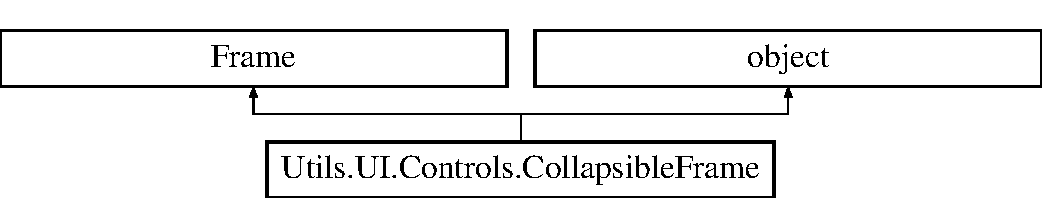
\includegraphics[height=2.000000cm]{class_c_utils_1_1_utils_1_1_u_i_1_1_controls_1_1_collapsible_frame}
\end{center}
\end{figure}
\subsection*{Public Member Functions}
\begin{DoxyCompactItemize}
\item 
\mbox{\Hypertarget{class_c_utils_1_1_utils_1_1_u_i_1_1_controls_1_1_collapsible_frame_a1fd54cca44098011a765116d40fc7fb1}\label{class_c_utils_1_1_utils_1_1_u_i_1_1_controls_1_1_collapsible_frame_a1fd54cca44098011a765116d40fc7fb1}} 
def {\bfseries \+\_\+\+\_\+init\+\_\+\+\_\+} (self, parent, text=None, borderwidth=2, width=0, height=16, interior\+\_\+padx=0, interior\+\_\+pady=18, background=None, caption\+\_\+separation=4, caption\+\_\+font=None, caption\+\_\+builder=None, icon\+\_\+x=5, icon\+\_\+open=None, icon\+\_\+close=None)
\item 
\mbox{\Hypertarget{class_c_utils_1_1_utils_1_1_u_i_1_1_controls_1_1_collapsible_frame_a4c1b4bd22aaabcfad76aad6823c25087}\label{class_c_utils_1_1_utils_1_1_u_i_1_1_controls_1_1_collapsible_frame_a4c1b4bd22aaabcfad76aad6823c25087}} 
def {\bfseries update\+\_\+width} (self, width=None)
\item 
\mbox{\Hypertarget{class_c_utils_1_1_utils_1_1_u_i_1_1_controls_1_1_collapsible_frame_a6a7ca114eeea12e38e719a070358ae14}\label{class_c_utils_1_1_utils_1_1_u_i_1_1_controls_1_1_collapsible_frame_a6a7ca114eeea12e38e719a070358ae14}} 
def {\bfseries open} (self)
\item 
\mbox{\Hypertarget{class_c_utils_1_1_utils_1_1_u_i_1_1_controls_1_1_collapsible_frame_a8639372c33e15084a7f7c4d9d87b7bfe}\label{class_c_utils_1_1_utils_1_1_u_i_1_1_controls_1_1_collapsible_frame_a8639372c33e15084a7f7c4d9d87b7bfe}} 
def {\bfseries close} (self)
\item 
\mbox{\Hypertarget{class_c_utils_1_1_utils_1_1_u_i_1_1_controls_1_1_collapsible_frame_a76ef2ebd71b1a1858194134725b6c800}\label{class_c_utils_1_1_utils_1_1_u_i_1_1_controls_1_1_collapsible_frame_a76ef2ebd71b1a1858194134725b6c800}} 
def {\bfseries toggle} (self)
\end{DoxyCompactItemize}
\subsection*{Public Attributes}
\begin{DoxyCompactItemize}
\item 
\mbox{\Hypertarget{class_c_utils_1_1_utils_1_1_u_i_1_1_controls_1_1_collapsible_frame_ae90f7328998ffbb9126e8c2db65049c5}\label{class_c_utils_1_1_utils_1_1_u_i_1_1_controls_1_1_collapsible_frame_ae90f7328998ffbb9126e8c2db65049c5}} 
{\bfseries interior}
\end{DoxyCompactItemize}


\subsection{Detailed Description}


Definition at line 548 of file C\+Utils.\+py.



The documentation for this class was generated from the following file\+:\begin{DoxyCompactItemize}
\item 
C\+Utils.\+py\end{DoxyCompactItemize}

\hypertarget{class_c_utils_1_1_utils_1_1_config}{}\section{Utils.\+Config Class Reference}
\label{class_c_utils_1_1_utils_1_1_config}\index{Utils.\+Config@{Utils.\+Config}}
\subsection*{Static Public Member Functions}
\begin{DoxyCompactItemize}
\item 
\mbox{\Hypertarget{class_c_utils_1_1_utils_1_1_config_a7de4021b6d5a4eb22be1439bfd497da8}\label{class_c_utils_1_1_utils_1_1_config_a7de4021b6d5a4eb22be1439bfd497da8}} 
def {\bfseries get\+Default\+Window\+Size} ()
\item 
\mbox{\Hypertarget{class_c_utils_1_1_utils_1_1_config_ae65cf338bda5bc527b1ace77855f0492}\label{class_c_utils_1_1_utils_1_1_config_ae65cf338bda5bc527b1ace77855f0492}} 
def {\bfseries get\+Window\+Title} ()
\item 
\mbox{\Hypertarget{class_c_utils_1_1_utils_1_1_config_a81185817b7a3d1bd7d5ce9bd22517541}\label{class_c_utils_1_1_utils_1_1_config_a81185817b7a3d1bd7d5ce9bd22517541}} 
def {\bfseries get\+App\+Location} ()
\item 
\mbox{\Hypertarget{class_c_utils_1_1_utils_1_1_config_a5fd0ae1aae4daaa4152b7407ff15e529}\label{class_c_utils_1_1_utils_1_1_config_a5fd0ae1aae4daaa4152b7407ff15e529}} 
def {\bfseries get\+Default\+Weather\+File} ()
\item 
\mbox{\Hypertarget{class_c_utils_1_1_utils_1_1_config_af548a638e3529545cd9b759510f8f9fd}\label{class_c_utils_1_1_utils_1_1_config_af548a638e3529545cd9b759510f8f9fd}} 
def {\bfseries get\+Default\+I\+DF} ()
\item 
\mbox{\Hypertarget{class_c_utils_1_1_utils_1_1_config_ac6c54378c1b87319af5bbb80031892e8}\label{class_c_utils_1_1_utils_1_1_config_ac6c54378c1b87319af5bbb80031892e8}} 
def {\bfseries get\+Default\+Output\+Directory} ()
\item 
\mbox{\Hypertarget{class_c_utils_1_1_utils_1_1_config_afdfd433c9e4b6c8ba7217773cdbd2893}\label{class_c_utils_1_1_utils_1_1_config_afdfd433c9e4b6c8ba7217773cdbd2893}} 
def {\bfseries get\+E\+Plus\+Location} ()
\item 
\mbox{\Hypertarget{class_c_utils_1_1_utils_1_1_config_a224e9f504a70979b42b2f9d8a15d80ed}\label{class_c_utils_1_1_utils_1_1_config_a224e9f504a70979b42b2f9d8a15d80ed}} 
def {\bfseries get\+Default\+Occupant\+Density} ()
\item 
\mbox{\Hypertarget{class_c_utils_1_1_utils_1_1_config_aaa46b72d973895fae7396bd7a676a9af}\label{class_c_utils_1_1_utils_1_1_config_aaa46b72d973895fae7396bd7a676a9af}} 
def {\bfseries get\+Value} (section, variable)
\item 
\mbox{\Hypertarget{class_c_utils_1_1_utils_1_1_config_a5df63f478e7412f05fd4341442d576f6}\label{class_c_utils_1_1_utils_1_1_config_a5df63f478e7412f05fd4341442d576f6}} 
def {\bfseries read\+Config\+File} (filename)
\item 
\mbox{\Hypertarget{class_c_utils_1_1_utils_1_1_config_a9c45e7f8346de6e1c36bfec816b5ad42}\label{class_c_utils_1_1_utils_1_1_config_a9c45e7f8346de6e1c36bfec816b5ad42}} 
def {\bfseries get\+Tooltip} (variable)
\item 
\mbox{\Hypertarget{class_c_utils_1_1_utils_1_1_config_a18fac3cac1d6e67a4d6bc52f062fd54e}\label{class_c_utils_1_1_utils_1_1_config_a18fac3cac1d6e67a4d6bc52f062fd54e}} 
def {\bfseries get\+Configuration\+File} (file\+Name, item=None)
\item 
\mbox{\Hypertarget{class_c_utils_1_1_utils_1_1_config_a17726dc36065d2005bdc7c6df88d84ad}\label{class_c_utils_1_1_utils_1_1_config_a17726dc36065d2005bdc7c6df88d84ad}} 
def {\bfseries get\+Configuration\+X\+M\+L\+File} (item=None)
\item 
\mbox{\Hypertarget{class_c_utils_1_1_utils_1_1_config_adeed3667616049a8d07e4ff6d0014bd3}\label{class_c_utils_1_1_utils_1_1_config_adeed3667616049a8d07e4ff6d0014bd3}} 
def {\bfseries get\+Agent\+Templates\+X\+M\+L\+File} (item=None)
\item 
def \hyperlink{class_c_utils_1_1_utils_1_1_config_a5e35e2165f66806e4eeb919eb148490b}{get\+Catalog} (sz\+Name, parent\+ID=None)
\begin{DoxyCompactList}\small\item\em Return list from the configuration file Return a list of options from the configuration file used in Drop\+Down\+List controls. \end{DoxyCompactList}\item 
\mbox{\Hypertarget{class_c_utils_1_1_utils_1_1_config_a20fa88fb99a7d1fe306a2b4aae7d5c15}\label{class_c_utils_1_1_utils_1_1_config_a20fa88fb99a7d1fe306a2b4aae7d5c15}} 
def {\bfseries get\+Collection} (sz\+Name)
\end{DoxyCompactItemize}


\subsection{Detailed Description}


Definition at line 88 of file C\+Utils.\+py.



\subsection{Member Function Documentation}
\mbox{\Hypertarget{class_c_utils_1_1_utils_1_1_config_a5e35e2165f66806e4eeb919eb148490b}\label{class_c_utils_1_1_utils_1_1_config_a5e35e2165f66806e4eeb919eb148490b}} 
\index{C\+Utils\+::\+Utils\+::\+Config@{C\+Utils\+::\+Utils\+::\+Config}!get\+Catalog@{get\+Catalog}}
\index{get\+Catalog@{get\+Catalog}!C\+Utils\+::\+Utils\+::\+Config@{C\+Utils\+::\+Utils\+::\+Config}}
\subsubsection{\texorpdfstring{get\+Catalog()}{getCatalog()}}
{\footnotesize\ttfamily def get\+Catalog (\begin{DoxyParamCaption}\item[{}]{sz\+Name,  }\item[{}]{parent\+ID = {\ttfamily None} }\end{DoxyParamCaption})\hspace{0.3cm}{\ttfamily [static]}}



Return list from the configuration file Return a list of options from the configuration file used in Drop\+Down\+List controls. 


\begin{DoxyParams}{Parameters}
{\em self} & \\
\hline
{\em sz\+Catalog} & Name of the list \\
\hline
{\em parent\+ID} & parent\+ID to filter the list chosen \\
\hline
\end{DoxyParams}


Definition at line 224 of file C\+Utils.\+py.



The documentation for this class was generated from the following file\+:\begin{DoxyCompactItemize}
\item 
C\+Utils.\+py\end{DoxyCompactItemize}

\hypertarget{class_c_utils_1_1_utils_1_1_constants}{}\section{Utils.\+Constants Class Reference}
\label{class_c_utils_1_1_utils_1_1_constants}\index{Utils.\+Constants@{Utils.\+Constants}}
\subsection*{Static Public Member Functions}
\begin{DoxyCompactItemize}
\item 
\mbox{\Hypertarget{class_c_utils_1_1_utils_1_1_constants_a957b3083d5f5b6db27830f9429d2d10b}\label{class_c_utils_1_1_utils_1_1_constants_a957b3083d5f5b6db27830f9429d2d10b}} 
def {\bfseries transparent\+Colour} ()
\end{DoxyCompactItemize}
\subsection*{Static Public Attributes}
\begin{DoxyCompactItemize}
\item 
\mbox{\Hypertarget{class_c_utils_1_1_utils_1_1_constants_a7c1ce2f7c84c7eb29d7a0b7660a419b2}\label{class_c_utils_1_1_utils_1_1_constants_a7c1ce2f7c84c7eb29d7a0b7660a419b2}} 
string {\bfseries empty\+G\+U\+ID} = \char`\"{}00000000-\/0000-\/0000-\/0000-\/000000000000\char`\"{}
\end{DoxyCompactItemize}


\subsection{Detailed Description}


Definition at line 28 of file C\+Utils.\+py.



The documentation for this class was generated from the following file\+:\begin{DoxyCompactItemize}
\item 
C\+Utils.\+py\end{DoxyCompactItemize}

\hypertarget{class_c_utils_1_1_utils_1_1_u_i_1_1_controls}{}\section{Utils.\+U\+I.\+Controls Class Reference}
\label{class_c_utils_1_1_utils_1_1_u_i_1_1_controls}\index{Utils.\+U\+I.\+Controls@{Utils.\+U\+I.\+Controls}}
\subsection*{Classes}
\begin{DoxyCompactItemize}
\item 
class \hyperlink{class_c_utils_1_1_utils_1_1_u_i_1_1_controls_1_1_auto_scroll_container}{Auto\+Scroll\+Container}
\item 
class \hyperlink{class_c_utils_1_1_utils_1_1_u_i_1_1_controls_1_1_cascading_drop_down_list}{Cascading\+Drop\+Down\+List}
\item 
class \hyperlink{class_c_utils_1_1_utils_1_1_u_i_1_1_controls_1_1_collapsible_frame}{Collapsible\+Frame}
\item 
class \hyperlink{class_c_utils_1_1_utils_1_1_u_i_1_1_controls_1_1_drop_down_list}{Drop\+Down\+List}
\item 
class \hyperlink{class_c_utils_1_1_utils_1_1_u_i_1_1_controls_1_1_lst_box}{Lst\+Box}
\item 
class \hyperlink{class_c_utils_1_1_utils_1_1_u_i_1_1_controls_1_1_scrollable_container}{Scrollable\+Container}
\item 
class \hyperlink{class_c_utils_1_1_utils_1_1_u_i_1_1_controls_1_1_scrolled_tree_view}{Scrolled\+Tree\+View}
\end{DoxyCompactItemize}
\subsection*{Static Public Member Functions}
\begin{DoxyCompactItemize}
\item 
\mbox{\Hypertarget{class_c_utils_1_1_utils_1_1_u_i_1_1_controls_afafd63786286cd84255ebd2392f6407a}\label{class_c_utils_1_1_utils_1_1_u_i_1_1_controls_afafd63786286cd84255ebd2392f6407a}} 
def {\bfseries Image\+Button} (parent, image\+Data, command, tool\+Tip=None)
\end{DoxyCompactItemize}


\subsection{Detailed Description}


Definition at line 330 of file C\+Utils.\+py.



The documentation for this class was generated from the following file\+:\begin{DoxyCompactItemize}
\item 
C\+Utils.\+py\end{DoxyCompactItemize}

\hypertarget{class_c_presence_1_1_c_presence}{}\section{C\+Presence Class Reference}
\label{class_c_presence_1_1_c_presence}\index{C\+Presence@{C\+Presence}}
Inheritance diagram for C\+Presence\+:\begin{figure}[H]
\begin{center}
\leavevmode
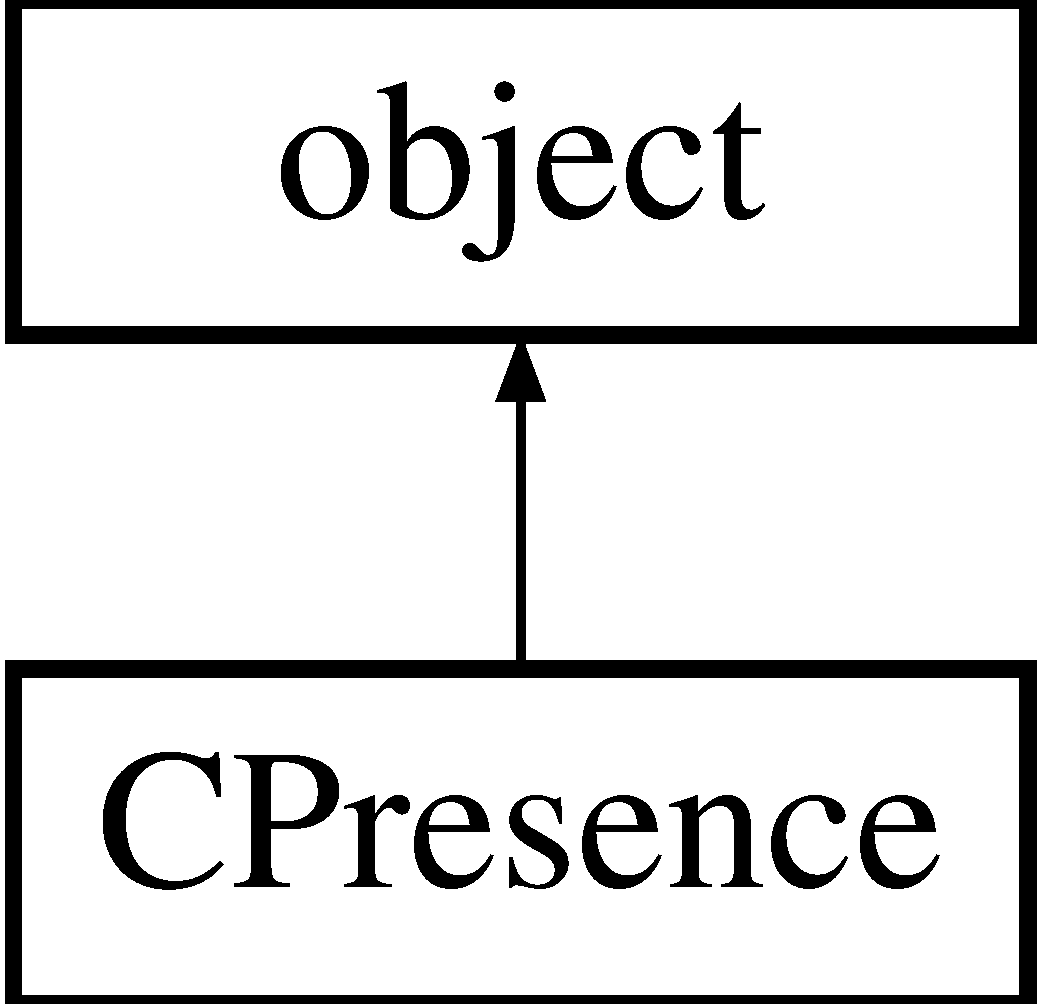
\includegraphics[height=2.000000cm]{class_c_presence_1_1_c_presence}
\end{center}
\end{figure}
\subsection*{Public Member Functions}
\begin{DoxyCompactItemize}
\item 
\mbox{\Hypertarget{class_c_presence_1_1_c_presence_abbcfc1a774079da020e49c42cbadb693}\label{class_c_presence_1_1_c_presence_abbcfc1a774079da020e49c42cbadb693}} 
def {\bfseries U\+U\+ID} (self)
\item 
\mbox{\Hypertarget{class_c_presence_1_1_c_presence_aff464267544e4efc9b770c8320c8f199}\label{class_c_presence_1_1_c_presence_aff464267544e4efc9b770c8320c8f199}} 
def {\bfseries type} (self)
\item 
\mbox{\Hypertarget{class_c_presence_1_1_c_presence_aca033702f187894894d3102de41d6b99}\label{class_c_presence_1_1_c_presence_aca033702f187894894d3102de41d6b99}} 
def {\bfseries type} (self, value)
\item 
\mbox{\Hypertarget{class_c_presence_1_1_c_presence_adb8818239148d2e5c5833a2b062ee9ad}\label{class_c_presence_1_1_c_presence_adb8818239148d2e5c5833a2b062ee9ad}} 
def {\bfseries ID} (self)
\item 
\mbox{\Hypertarget{class_c_presence_1_1_c_presence_a0a178fbcae3f6431733dd63ee37ac7bb}\label{class_c_presence_1_1_c_presence_a0a178fbcae3f6431733dd63ee37ac7bb}} 
def {\bfseries ID} (self, value)
\item 
\mbox{\Hypertarget{class_c_presence_1_1_c_presence_a05cd4cd28b324f262fefe1a1782bd992}\label{class_c_presence_1_1_c_presence_a05cd4cd28b324f262fefe1a1782bd992}} 
def {\bfseries enabled} (self)
\item 
\mbox{\Hypertarget{class_c_presence_1_1_c_presence_a18495e0c3f2639c84751c9aa77cd03b3}\label{class_c_presence_1_1_c_presence_a18495e0c3f2639c84751c9aa77cd03b3}} 
def {\bfseries enabled} (self, value)
\item 
\mbox{\Hypertarget{class_c_presence_1_1_c_presence_a71963b9940a29bf3f2c10546c2cb9b50}\label{class_c_presence_1_1_c_presence_a71963b9940a29bf3f2c10546c2cb9b50}} 
def {\bfseries \+\_\+\+\_\+init\+\_\+\+\_\+} (self, id=str(uuid.\+uuid4()), enabled=True)
\end{DoxyCompactItemize}


\subsection{Detailed Description}


Definition at line 12 of file C\+Presence.\+py.



The documentation for this class was generated from the following file\+:\begin{DoxyCompactItemize}
\item 
C\+Presence.\+py\end{DoxyCompactItemize}

\hypertarget{class_c_shade_1_1_c_shade}{}\section{C\+Shade Class Reference}
\label{class_c_shade_1_1_c_shade}\index{C\+Shade@{C\+Shade}}
Inheritance diagram for C\+Shade\+:\begin{figure}[H]
\begin{center}
\leavevmode
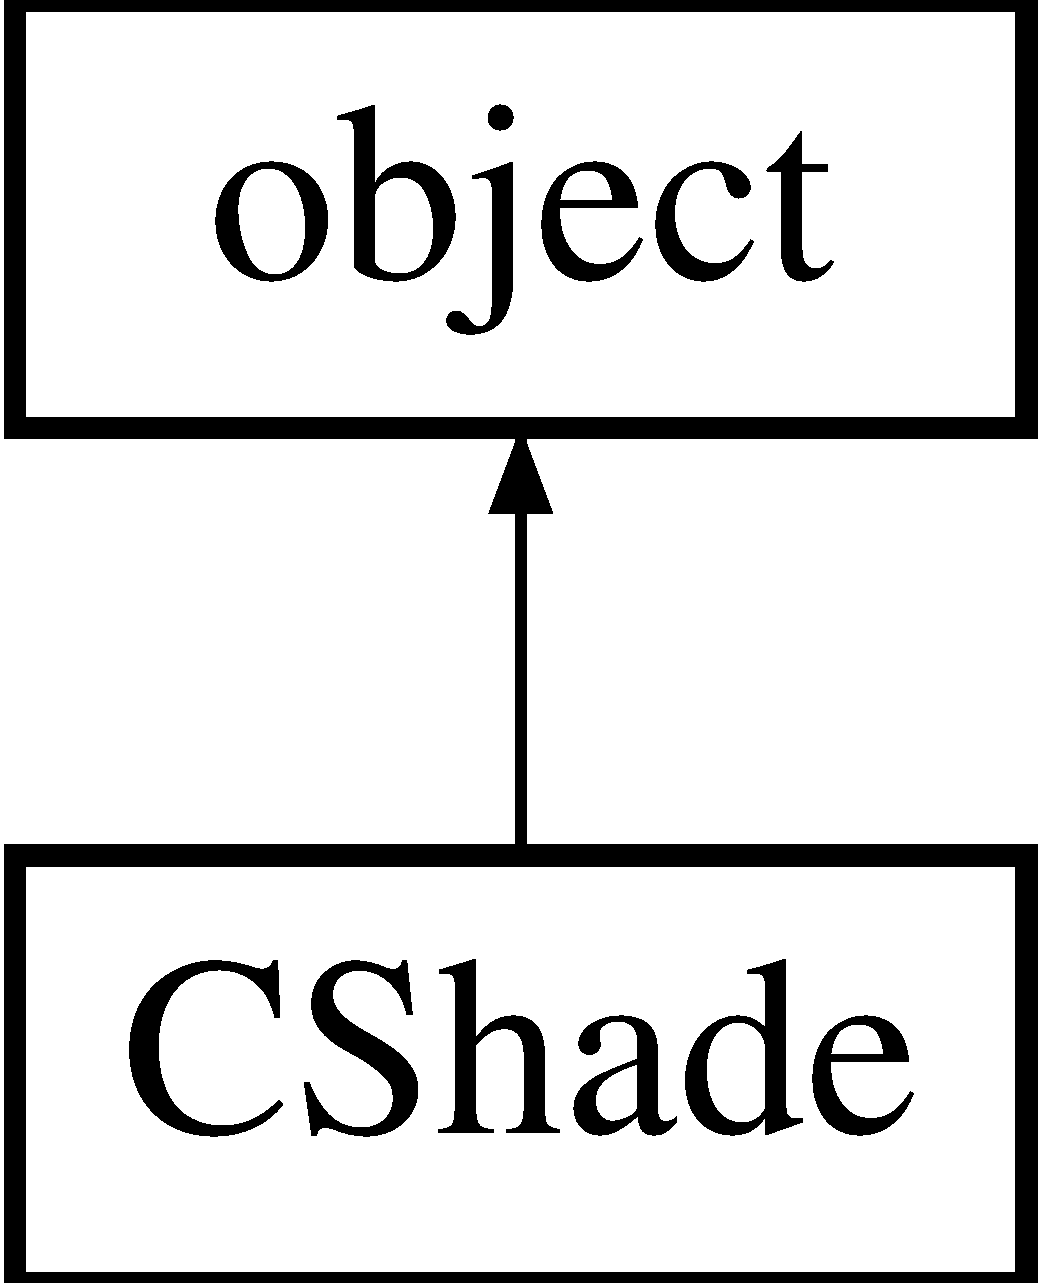
\includegraphics[height=2.000000cm]{class_c_shade_1_1_c_shade}
\end{center}
\end{figure}
\subsection*{Public Member Functions}
\begin{DoxyCompactItemize}
\item 
\mbox{\Hypertarget{class_c_shade_1_1_c_shade_abbcfc1a774079da020e49c42cbadb693}\label{class_c_shade_1_1_c_shade_abbcfc1a774079da020e49c42cbadb693}} 
def {\bfseries U\+U\+ID} (self)
\item 
\mbox{\Hypertarget{class_c_shade_1_1_c_shade_aff464267544e4efc9b770c8320c8f199}\label{class_c_shade_1_1_c_shade_aff464267544e4efc9b770c8320c8f199}} 
def {\bfseries type} (self)
\item 
\mbox{\Hypertarget{class_c_shade_1_1_c_shade_aca033702f187894894d3102de41d6b99}\label{class_c_shade_1_1_c_shade_aca033702f187894894d3102de41d6b99}} 
def {\bfseries type} (self, value)
\item 
\mbox{\Hypertarget{class_c_shade_1_1_c_shade_adb8818239148d2e5c5833a2b062ee9ad}\label{class_c_shade_1_1_c_shade_adb8818239148d2e5c5833a2b062ee9ad}} 
def {\bfseries ID} (self)
\item 
\mbox{\Hypertarget{class_c_shade_1_1_c_shade_a0a178fbcae3f6431733dd63ee37ac7bb}\label{class_c_shade_1_1_c_shade_a0a178fbcae3f6431733dd63ee37ac7bb}} 
def {\bfseries ID} (self, value)
\item 
\mbox{\Hypertarget{class_c_shade_1_1_c_shade_a5907ca3bbf8e7cd8f40c3007338f6d02}\label{class_c_shade_1_1_c_shade_a5907ca3bbf8e7cd8f40c3007338f6d02}} 
def {\bfseries name} (self)
\item 
\mbox{\Hypertarget{class_c_shade_1_1_c_shade_a62d212fdcbbcee30e90a64ce349d32f8}\label{class_c_shade_1_1_c_shade_a62d212fdcbbcee30e90a64ce349d32f8}} 
def {\bfseries name} (self, value)
\item 
\mbox{\Hypertarget{class_c_shade_1_1_c_shade_afbd784f4e474831ced93fb7de372fa86}\label{class_c_shade_1_1_c_shade_afbd784f4e474831ced93fb7de372fa86}} 
def {\bfseries a01arr} (self)
\item 
\mbox{\Hypertarget{class_c_shade_1_1_c_shade_a48d0c7289e796d29301c52be0ec20e61}\label{class_c_shade_1_1_c_shade_a48d0c7289e796d29301c52be0ec20e61}} 
def {\bfseries a01arr} (self, value)
\item 
\mbox{\Hypertarget{class_c_shade_1_1_c_shade_a1e2fd05578440dee4b4d92ebd044372d}\label{class_c_shade_1_1_c_shade_a1e2fd05578440dee4b4d92ebd044372d}} 
def {\bfseries b01inarr} (self)
\item 
\mbox{\Hypertarget{class_c_shade_1_1_c_shade_a7ab1eadd41a73dec8eb72f7f5d099c9a}\label{class_c_shade_1_1_c_shade_a7ab1eadd41a73dec8eb72f7f5d099c9a}} 
def {\bfseries b01inarr} (self, value)
\item 
\mbox{\Hypertarget{class_c_shade_1_1_c_shade_ab76aae1ec6b3b44c45962e8f7c0d7f67}\label{class_c_shade_1_1_c_shade_ab76aae1ec6b3b44c45962e8f7c0d7f67}} 
def {\bfseries b01sarr} (self)
\item 
\mbox{\Hypertarget{class_c_shade_1_1_c_shade_a3437517df65438836403ba3a691da314}\label{class_c_shade_1_1_c_shade_a3437517df65438836403ba3a691da314}} 
def {\bfseries b01sarr} (self, value)
\item 
\mbox{\Hypertarget{class_c_shade_1_1_c_shade_aa3a37e286de481cad594e8b9d647bd2d}\label{class_c_shade_1_1_c_shade_aa3a37e286de481cad594e8b9d647bd2d}} 
def {\bfseries a10arr} (self)
\item 
\mbox{\Hypertarget{class_c_shade_1_1_c_shade_a2e0fef132160af93ff1dead7eb454327}\label{class_c_shade_1_1_c_shade_a2e0fef132160af93ff1dead7eb454327}} 
def {\bfseries a10arr} (self, value)
\item 
\mbox{\Hypertarget{class_c_shade_1_1_c_shade_a9650430b18b9d1766ac2743902835dfc}\label{class_c_shade_1_1_c_shade_a9650430b18b9d1766ac2743902835dfc}} 
def {\bfseries b10inarr} (self)
\item 
\mbox{\Hypertarget{class_c_shade_1_1_c_shade_a24fe47109103b234c5dd4f0a482bfa1c}\label{class_c_shade_1_1_c_shade_a24fe47109103b234c5dd4f0a482bfa1c}} 
def {\bfseries b10inarr} (self, value)
\item 
\mbox{\Hypertarget{class_c_shade_1_1_c_shade_afd658cacee848a09a4872fbae00cc098}\label{class_c_shade_1_1_c_shade_afd658cacee848a09a4872fbae00cc098}} 
def {\bfseries b10sarr} (self)
\item 
\mbox{\Hypertarget{class_c_shade_1_1_c_shade_ad36f645998ba1987163c2ff848c67800}\label{class_c_shade_1_1_c_shade_ad36f645998ba1987163c2ff848c67800}} 
def {\bfseries b10sarr} (self, value)
\item 
\mbox{\Hypertarget{class_c_shade_1_1_c_shade_afdc87f94ba621dccb191d97c935460fa}\label{class_c_shade_1_1_c_shade_afdc87f94ba621dccb191d97c935460fa}} 
def {\bfseries a01int} (self)
\item 
\mbox{\Hypertarget{class_c_shade_1_1_c_shade_ad148d326b6c966955e5e97b45d49557c}\label{class_c_shade_1_1_c_shade_ad148d326b6c966955e5e97b45d49557c}} 
def {\bfseries a01int} (self, value)
\item 
\mbox{\Hypertarget{class_c_shade_1_1_c_shade_a2f658eef72d2dea1337c1c999e066a49}\label{class_c_shade_1_1_c_shade_a2f658eef72d2dea1337c1c999e066a49}} 
def {\bfseries b01inint} (self)
\item 
\mbox{\Hypertarget{class_c_shade_1_1_c_shade_a3a43006698c7a7484b7f9c0f556e934a}\label{class_c_shade_1_1_c_shade_a3a43006698c7a7484b7f9c0f556e934a}} 
def {\bfseries b01inint} (self, value)
\item 
\mbox{\Hypertarget{class_c_shade_1_1_c_shade_a3fc66f4d0e88985c912d5fa71575615c}\label{class_c_shade_1_1_c_shade_a3fc66f4d0e88985c912d5fa71575615c}} 
def {\bfseries b01sint} (self)
\item 
\mbox{\Hypertarget{class_c_shade_1_1_c_shade_a83108599e567a451c3c66dcfbf712f33}\label{class_c_shade_1_1_c_shade_a83108599e567a451c3c66dcfbf712f33}} 
def {\bfseries b01sint} (self, value)
\item 
\mbox{\Hypertarget{class_c_shade_1_1_c_shade_a564c1e1d3ef5a53e335539bb781b0055}\label{class_c_shade_1_1_c_shade_a564c1e1d3ef5a53e335539bb781b0055}} 
def {\bfseries a10int} (self)
\item 
\mbox{\Hypertarget{class_c_shade_1_1_c_shade_a350fe6cb6a7e1a780cb3027db163d7bb}\label{class_c_shade_1_1_c_shade_a350fe6cb6a7e1a780cb3027db163d7bb}} 
def {\bfseries a10int} (self, value)
\item 
\mbox{\Hypertarget{class_c_shade_1_1_c_shade_ac254f58dfa27d9cde927964241fdcdff}\label{class_c_shade_1_1_c_shade_ac254f58dfa27d9cde927964241fdcdff}} 
def {\bfseries b10inint} (self)
\item 
\mbox{\Hypertarget{class_c_shade_1_1_c_shade_acfa867358731f24582bfafe19b59f8a3}\label{class_c_shade_1_1_c_shade_acfa867358731f24582bfafe19b59f8a3}} 
def {\bfseries b10inint} (self, value)
\item 
\mbox{\Hypertarget{class_c_shade_1_1_c_shade_ae6c407db8095f20f9808ee387a03a7f5}\label{class_c_shade_1_1_c_shade_ae6c407db8095f20f9808ee387a03a7f5}} 
def {\bfseries b10sint} (self)
\item 
\mbox{\Hypertarget{class_c_shade_1_1_c_shade_ad1a6ffcba313308a6b81ac2cf25b81fd}\label{class_c_shade_1_1_c_shade_ad1a6ffcba313308a6b81ac2cf25b81fd}} 
def {\bfseries b10sint} (self, value)
\item 
\mbox{\Hypertarget{class_c_shade_1_1_c_shade_ac896011df626c98b6bc7a012bcf83cb6}\label{class_c_shade_1_1_c_shade_ac896011df626c98b6bc7a012bcf83cb6}} 
def {\bfseries afullraise} (self)
\item 
\mbox{\Hypertarget{class_c_shade_1_1_c_shade_a93999fb10adbe2667c95dfca81aedf55}\label{class_c_shade_1_1_c_shade_a93999fb10adbe2667c95dfca81aedf55}} 
def {\bfseries afullraise} (self, value)
\item 
\mbox{\Hypertarget{class_c_shade_1_1_c_shade_ab69d95a4d2a64c7b02a3f52fa5212d2b}\label{class_c_shade_1_1_c_shade_ab69d95a4d2a64c7b02a3f52fa5212d2b}} 
def {\bfseries boutfullraise} (self)
\item 
\mbox{\Hypertarget{class_c_shade_1_1_c_shade_ac60673dde91aa368547cede2de6fbb50}\label{class_c_shade_1_1_c_shade_ac60673dde91aa368547cede2de6fbb50}} 
def {\bfseries boutfullraise} (self, value)
\item 
\mbox{\Hypertarget{class_c_shade_1_1_c_shade_aa1670f241bbee1d6598b4d74bc5da496}\label{class_c_shade_1_1_c_shade_aa1670f241bbee1d6598b4d74bc5da496}} 
def {\bfseries bsfullraise} (self)
\item 
\mbox{\Hypertarget{class_c_shade_1_1_c_shade_ac56d11c8c1a65aa24d056d2e75b59c9a}\label{class_c_shade_1_1_c_shade_ac56d11c8c1a65aa24d056d2e75b59c9a}} 
def {\bfseries bsfullraise} (self, value)
\item 
\mbox{\Hypertarget{class_c_shade_1_1_c_shade_a1004024fe652b68066983ce67ff39562}\label{class_c_shade_1_1_c_shade_a1004024fe652b68066983ce67ff39562}} 
def {\bfseries bsfulllower} (self)
\item 
\mbox{\Hypertarget{class_c_shade_1_1_c_shade_a0ba562b4d174147e6bccd419682378dd}\label{class_c_shade_1_1_c_shade_a0ba562b4d174147e6bccd419682378dd}} 
def {\bfseries bsfulllower} (self, value)
\item 
\mbox{\Hypertarget{class_c_shade_1_1_c_shade_a43b7b774fae7dd6f7535956132c4f4a7}\label{class_c_shade_1_1_c_shade_a43b7b774fae7dd6f7535956132c4f4a7}} 
def {\bfseries boutfulllower} (self)
\item 
\mbox{\Hypertarget{class_c_shade_1_1_c_shade_af2bc1562bcdff1fd26653705bbf80209}\label{class_c_shade_1_1_c_shade_af2bc1562bcdff1fd26653705bbf80209}} 
def {\bfseries boutfulllower} (self, value)
\item 
\mbox{\Hypertarget{class_c_shade_1_1_c_shade_af93bd56f25b4e7b72fade8017b0c45ea}\label{class_c_shade_1_1_c_shade_af93bd56f25b4e7b72fade8017b0c45ea}} 
def {\bfseries afulllower} (self)
\item 
\mbox{\Hypertarget{class_c_shade_1_1_c_shade_ac7a6c299368a7215c61097d17453a7b1}\label{class_c_shade_1_1_c_shade_ac7a6c299368a7215c61097d17453a7b1}} 
def {\bfseries afulllower} (self, value)
\item 
\mbox{\Hypertarget{class_c_shade_1_1_c_shade_ade80e7fc571d60c992453d3813d53301}\label{class_c_shade_1_1_c_shade_ade80e7fc571d60c992453d3813d53301}} 
def {\bfseries a\+S\+Flower} (self)
\item 
\mbox{\Hypertarget{class_c_shade_1_1_c_shade_a679f471062d45004a3965572249375c1}\label{class_c_shade_1_1_c_shade_a679f471062d45004a3965572249375c1}} 
def {\bfseries a\+S\+Flower} (self, value)
\item 
\mbox{\Hypertarget{class_c_shade_1_1_c_shade_a2f96183890fed63e015e5d7580ffa296}\label{class_c_shade_1_1_c_shade_a2f96183890fed63e015e5d7580ffa296}} 
def {\bfseries b\+S\+Flower} (self)
\item 
\mbox{\Hypertarget{class_c_shade_1_1_c_shade_a77cde65eacdddc528337b7ed6586b2ef}\label{class_c_shade_1_1_c_shade_a77cde65eacdddc528337b7ed6586b2ef}} 
def {\bfseries b\+S\+Flower} (self, value)
\item 
\mbox{\Hypertarget{class_c_shade_1_1_c_shade_a87593a9edc4c21f7b5acde8a0d339586}\label{class_c_shade_1_1_c_shade_a87593a9edc4c21f7b5acde8a0d339586}} 
def {\bfseries shapelower} (self)
\item 
\mbox{\Hypertarget{class_c_shade_1_1_c_shade_ac8bf9586187ba8191a3c61593ed622f3}\label{class_c_shade_1_1_c_shade_ac8bf9586187ba8191a3c61593ed622f3}} 
def {\bfseries shapelower} (self, value)
\item 
\mbox{\Hypertarget{class_c_shade_1_1_c_shade_aecfe92e74f185bbe044724fc20ff0e0e}\label{class_c_shade_1_1_c_shade_aecfe92e74f185bbe044724fc20ff0e0e}} 
def {\bfseries \+\_\+\+\_\+init\+\_\+\+\_\+} (self, id=0, name=\textquotesingle{}\textquotesingle{}, a01arr=0, b01inarr=0, b01sarr=0, a10arr=0, b10inarr=0, b10sarr=0, a01int=0, b01inint=0, b01sint=0, a10int=0, b10inint=0, b10sint=0, afullraise=0, boutfullraise=0, bsfullraise=0, bsfulllower=0, boutfulllower=0, afulllower=0, a\+S\+Flower=0, b\+S\+Flower=0, shapelower=0)
\end{DoxyCompactItemize}


\subsection{Detailed Description}


Definition at line 12 of file C\+Shade.\+py.



The documentation for this class was generated from the following file\+:\begin{DoxyCompactItemize}
\item 
C\+Shade.\+py\end{DoxyCompactItemize}

\hypertarget{class_c_shades_1_1_c_shades}{}\section{C\+Shades Class Reference}
\label{class_c_shades_1_1_c_shades}\index{C\+Shades@{C\+Shades}}
Inheritance diagram for C\+Shades\+:\begin{figure}[H]
\begin{center}
\leavevmode
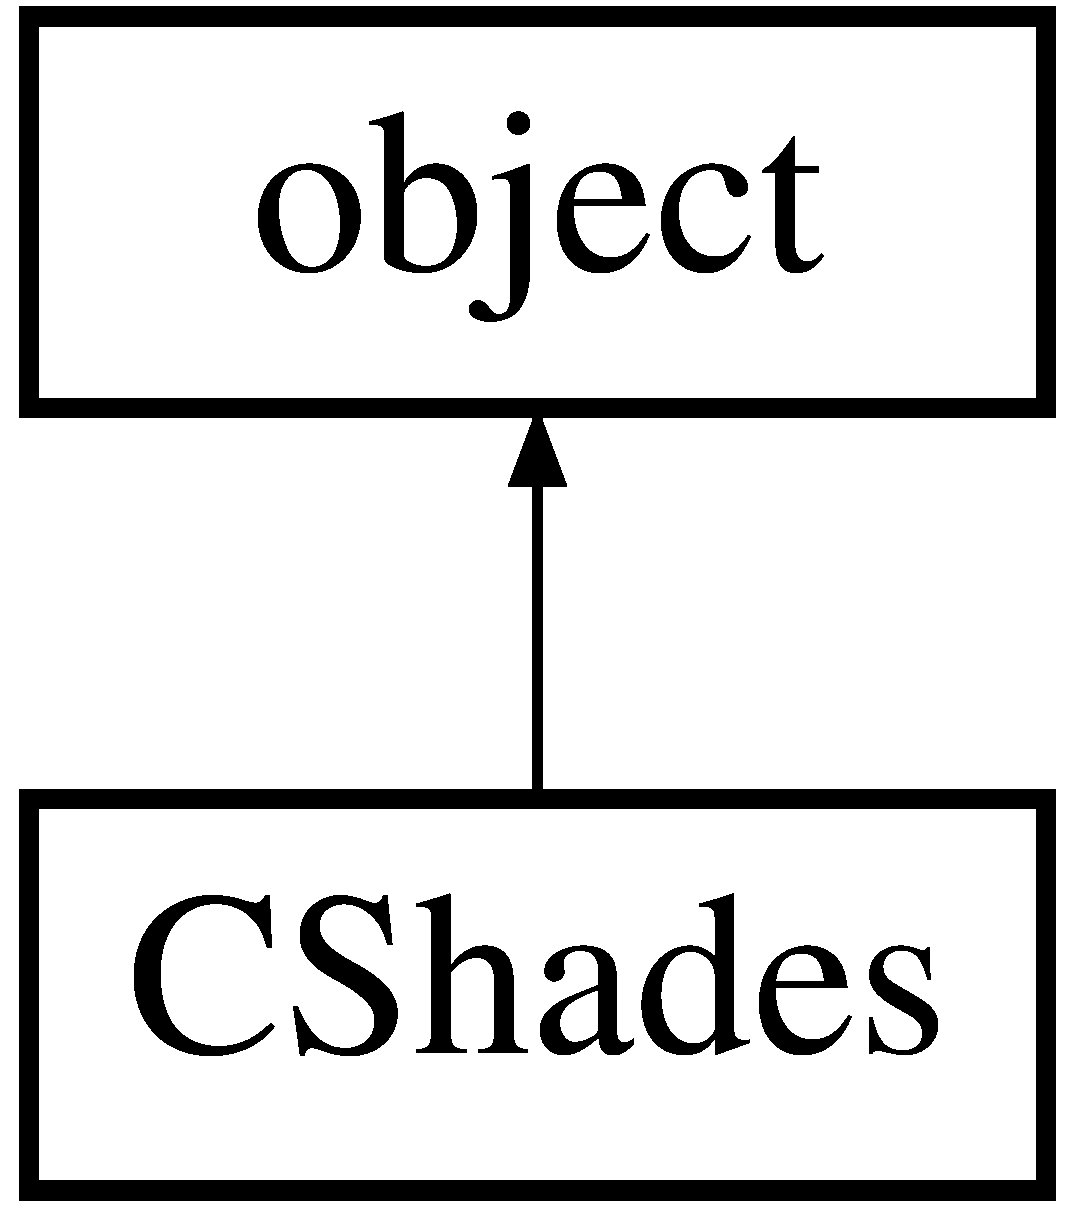
\includegraphics[height=2.000000cm]{class_c_shades_1_1_c_shades}
\end{center}
\end{figure}
\subsection*{Public Member Functions}
\begin{DoxyCompactItemize}
\item 
\mbox{\Hypertarget{class_c_shades_1_1_c_shades_abbcfc1a774079da020e49c42cbadb693}\label{class_c_shades_1_1_c_shades_abbcfc1a774079da020e49c42cbadb693}} 
def {\bfseries U\+U\+ID} (self)
\item 
\mbox{\Hypertarget{class_c_shades_1_1_c_shades_aff464267544e4efc9b770c8320c8f199}\label{class_c_shades_1_1_c_shades_aff464267544e4efc9b770c8320c8f199}} 
def {\bfseries type} (self)
\item 
\mbox{\Hypertarget{class_c_shades_1_1_c_shades_aca033702f187894894d3102de41d6b99}\label{class_c_shades_1_1_c_shades_aca033702f187894894d3102de41d6b99}} 
def {\bfseries type} (self, value)
\item 
\mbox{\Hypertarget{class_c_shades_1_1_c_shades_adb8818239148d2e5c5833a2b062ee9ad}\label{class_c_shades_1_1_c_shades_adb8818239148d2e5c5833a2b062ee9ad}} 
def {\bfseries ID} (self)
\item 
\mbox{\Hypertarget{class_c_shades_1_1_c_shades_a0a178fbcae3f6431733dd63ee37ac7bb}\label{class_c_shades_1_1_c_shades_a0a178fbcae3f6431733dd63ee37ac7bb}} 
def {\bfseries ID} (self, value)
\item 
\mbox{\Hypertarget{class_c_shades_1_1_c_shades_a05cd4cd28b324f262fefe1a1782bd992}\label{class_c_shades_1_1_c_shades_a05cd4cd28b324f262fefe1a1782bd992}} 
def {\bfseries enabled} (self)
\item 
\mbox{\Hypertarget{class_c_shades_1_1_c_shades_a18495e0c3f2639c84751c9aa77cd03b3}\label{class_c_shades_1_1_c_shades_a18495e0c3f2639c84751c9aa77cd03b3}} 
def {\bfseries enabled} (self, value)
\item 
\mbox{\Hypertarget{class_c_shades_1_1_c_shades_a71963b9940a29bf3f2c10546c2cb9b50}\label{class_c_shades_1_1_c_shades_a71963b9940a29bf3f2c10546c2cb9b50}} 
def {\bfseries \+\_\+\+\_\+init\+\_\+\+\_\+} (self, id=str(uuid.\+uuid4()), enabled=True)
\end{DoxyCompactItemize}


\subsection{Detailed Description}


Definition at line 12 of file C\+Shades.\+py.



The documentation for this class was generated from the following file\+:\begin{DoxyCompactItemize}
\item 
C\+Shades.\+py\end{DoxyCompactItemize}

\hypertarget{class_c_window_1_1_c_window}{}\section{C\+Window Class Reference}
\label{class_c_window_1_1_c_window}\index{C\+Window@{C\+Window}}
Inheritance diagram for C\+Window\+:\begin{figure}[H]
\begin{center}
\leavevmode
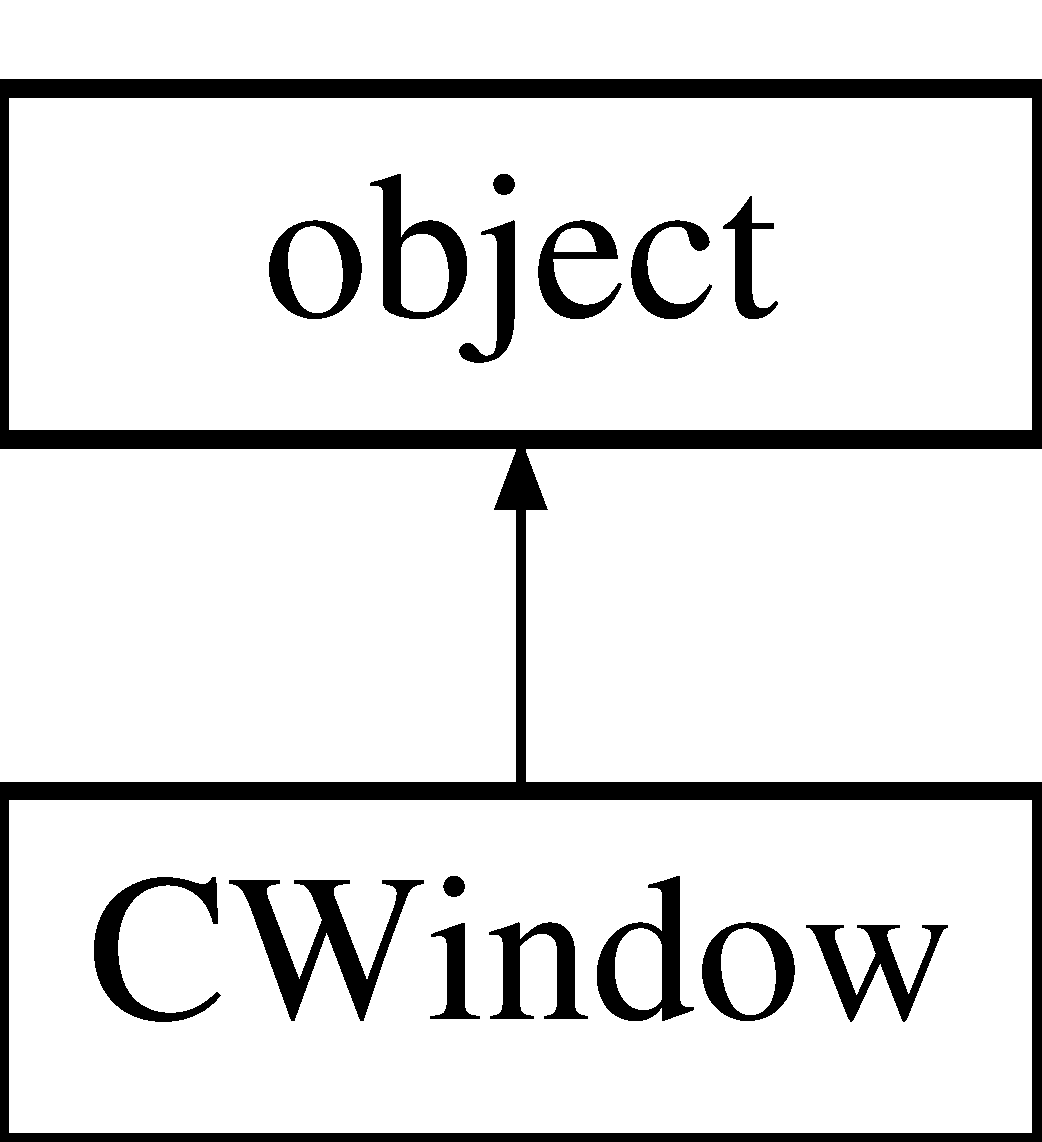
\includegraphics[height=2.000000cm]{class_c_window_1_1_c_window}
\end{center}
\end{figure}
\subsection*{Public Member Functions}
\begin{DoxyCompactItemize}
\item 
\mbox{\Hypertarget{class_c_window_1_1_c_window_abbcfc1a774079da020e49c42cbadb693}\label{class_c_window_1_1_c_window_abbcfc1a774079da020e49c42cbadb693}} 
def {\bfseries U\+U\+ID} (self)
\item 
\mbox{\Hypertarget{class_c_window_1_1_c_window_aff464267544e4efc9b770c8320c8f199}\label{class_c_window_1_1_c_window_aff464267544e4efc9b770c8320c8f199}} 
def {\bfseries type} (self)
\item 
\mbox{\Hypertarget{class_c_window_1_1_c_window_aca033702f187894894d3102de41d6b99}\label{class_c_window_1_1_c_window_aca033702f187894894d3102de41d6b99}} 
def {\bfseries type} (self, value)
\item 
\mbox{\Hypertarget{class_c_window_1_1_c_window_adb8818239148d2e5c5833a2b062ee9ad}\label{class_c_window_1_1_c_window_adb8818239148d2e5c5833a2b062ee9ad}} 
def {\bfseries ID} (self)
\item 
\mbox{\Hypertarget{class_c_window_1_1_c_window_a0a178fbcae3f6431733dd63ee37ac7bb}\label{class_c_window_1_1_c_window_a0a178fbcae3f6431733dd63ee37ac7bb}} 
def {\bfseries ID} (self, value)
\item 
\mbox{\Hypertarget{class_c_window_1_1_c_window_a5907ca3bbf8e7cd8f40c3007338f6d02}\label{class_c_window_1_1_c_window_a5907ca3bbf8e7cd8f40c3007338f6d02}} 
def {\bfseries name} (self)
\item 
\mbox{\Hypertarget{class_c_window_1_1_c_window_a62d212fdcbbcee30e90a64ce349d32f8}\label{class_c_window_1_1_c_window_a62d212fdcbbcee30e90a64ce349d32f8}} 
def {\bfseries name} (self, value)
\item 
\mbox{\Hypertarget{class_c_window_1_1_c_window_a1bc2c7a7aeb532bfa8bf834ec0cfb630}\label{class_c_window_1_1_c_window_a1bc2c7a7aeb532bfa8bf834ec0cfb630}} 
def {\bfseries aop} (self)
\item 
\mbox{\Hypertarget{class_c_window_1_1_c_window_a7b79dd107f69c89d0b01f7b7a8d41603}\label{class_c_window_1_1_c_window_a7b79dd107f69c89d0b01f7b7a8d41603}} 
def {\bfseries aop} (self, value)
\item 
\mbox{\Hypertarget{class_c_window_1_1_c_window_a4cb8c39fee6878d719aa6d7e8b6cde39}\label{class_c_window_1_1_c_window_a4cb8c39fee6878d719aa6d7e8b6cde39}} 
def {\bfseries bopout} (self)
\item 
\mbox{\Hypertarget{class_c_window_1_1_c_window_a992cedbc774abaec307a9d9cedd1601b}\label{class_c_window_1_1_c_window_a992cedbc774abaec307a9d9cedd1601b}} 
def {\bfseries bopout} (self, value)
\item 
\mbox{\Hypertarget{class_c_window_1_1_c_window_ac7235dd8ae8c9189f21adceaf8a2efa9}\label{class_c_window_1_1_c_window_ac7235dd8ae8c9189f21adceaf8a2efa9}} 
def {\bfseries shapeop} (self)
\item 
\mbox{\Hypertarget{class_c_window_1_1_c_window_aec57ee95613e0846bd7bc978665ca887}\label{class_c_window_1_1_c_window_aec57ee95613e0846bd7bc978665ca887}} 
def {\bfseries shapeop} (self, value)
\item 
\mbox{\Hypertarget{class_c_window_1_1_c_window_afbd784f4e474831ced93fb7de372fa86}\label{class_c_window_1_1_c_window_afbd784f4e474831ced93fb7de372fa86}} 
def {\bfseries a01arr} (self)
\item 
\mbox{\Hypertarget{class_c_window_1_1_c_window_a48d0c7289e796d29301c52be0ec20e61}\label{class_c_window_1_1_c_window_a48d0c7289e796d29301c52be0ec20e61}} 
def {\bfseries a01arr} (self, value)
\item 
\mbox{\Hypertarget{class_c_window_1_1_c_window_a1e2fd05578440dee4b4d92ebd044372d}\label{class_c_window_1_1_c_window_a1e2fd05578440dee4b4d92ebd044372d}} 
def {\bfseries b01inarr} (self)
\item 
\mbox{\Hypertarget{class_c_window_1_1_c_window_a7ab1eadd41a73dec8eb72f7f5d099c9a}\label{class_c_window_1_1_c_window_a7ab1eadd41a73dec8eb72f7f5d099c9a}} 
def {\bfseries b01inarr} (self, value)
\item 
\mbox{\Hypertarget{class_c_window_1_1_c_window_aed415aa8b030e4e9225e4385b05e4efe}\label{class_c_window_1_1_c_window_aed415aa8b030e4e9225e4385b05e4efe}} 
def {\bfseries b01outarr} (self)
\item 
\mbox{\Hypertarget{class_c_window_1_1_c_window_a77b844e4e3f5205e34a8cbd88633430f}\label{class_c_window_1_1_c_window_a77b844e4e3f5205e34a8cbd88633430f}} 
def {\bfseries b01outarr} (self, value)
\item 
\mbox{\Hypertarget{class_c_window_1_1_c_window_aaa1a0a0fec2d472660ed2bbb95755b07}\label{class_c_window_1_1_c_window_aaa1a0a0fec2d472660ed2bbb95755b07}} 
def {\bfseries b01absprevarr} (self)
\item 
\mbox{\Hypertarget{class_c_window_1_1_c_window_ae06fc310b30a72d8677c18b6e6e251a5}\label{class_c_window_1_1_c_window_ae06fc310b30a72d8677c18b6e6e251a5}} 
def {\bfseries b01absprevarr} (self, value)
\item 
\mbox{\Hypertarget{class_c_window_1_1_c_window_a39a4fe8cfcc0dfc2a5ddd40c2fb9ce9b}\label{class_c_window_1_1_c_window_a39a4fe8cfcc0dfc2a5ddd40c2fb9ce9b}} 
def {\bfseries b01rnarr} (self)
\item 
\mbox{\Hypertarget{class_c_window_1_1_c_window_ac3a3e094fa57b5f4abe8ad59d5aedd9e}\label{class_c_window_1_1_c_window_ac3a3e094fa57b5f4abe8ad59d5aedd9e}} 
def {\bfseries b01rnarr} (self, value)
\item 
\mbox{\Hypertarget{class_c_window_1_1_c_window_afdc87f94ba621dccb191d97c935460fa}\label{class_c_window_1_1_c_window_afdc87f94ba621dccb191d97c935460fa}} 
def {\bfseries a01int} (self)
\item 
\mbox{\Hypertarget{class_c_window_1_1_c_window_ad148d326b6c966955e5e97b45d49557c}\label{class_c_window_1_1_c_window_ad148d326b6c966955e5e97b45d49557c}} 
def {\bfseries a01int} (self, value)
\item 
\mbox{\Hypertarget{class_c_window_1_1_c_window_a2f658eef72d2dea1337c1c999e066a49}\label{class_c_window_1_1_c_window_a2f658eef72d2dea1337c1c999e066a49}} 
def {\bfseries b01inint} (self)
\item 
\mbox{\Hypertarget{class_c_window_1_1_c_window_a3a43006698c7a7484b7f9c0f556e934a}\label{class_c_window_1_1_c_window_a3a43006698c7a7484b7f9c0f556e934a}} 
def {\bfseries b01inint} (self, value)
\item 
\mbox{\Hypertarget{class_c_window_1_1_c_window_a532a45faf2e76c7a1b3b64d0b674fc88}\label{class_c_window_1_1_c_window_a532a45faf2e76c7a1b3b64d0b674fc88}} 
def {\bfseries b01outint} (self)
\item 
\mbox{\Hypertarget{class_c_window_1_1_c_window_a0b5739b13c2dd7e359ed8765036502c1}\label{class_c_window_1_1_c_window_a0b5739b13c2dd7e359ed8765036502c1}} 
def {\bfseries b01outint} (self, value)
\item 
\mbox{\Hypertarget{class_c_window_1_1_c_window_a1c832d04506a1cd176054e300c873193}\label{class_c_window_1_1_c_window_a1c832d04506a1cd176054e300c873193}} 
def {\bfseries b01presint} (self)
\item 
\mbox{\Hypertarget{class_c_window_1_1_c_window_a4c2e32bd052f39a69913782f277a93b2}\label{class_c_window_1_1_c_window_a4c2e32bd052f39a69913782f277a93b2}} 
def {\bfseries b01presint} (self, value)
\item 
\mbox{\Hypertarget{class_c_window_1_1_c_window_a87141db51cdf14799a9946c83810c12e}\label{class_c_window_1_1_c_window_a87141db51cdf14799a9946c83810c12e}} 
def {\bfseries b01rnint} (self)
\item 
\mbox{\Hypertarget{class_c_window_1_1_c_window_a9fba7cd741a1edcd2ca2474c0de45f91}\label{class_c_window_1_1_c_window_a9fba7cd741a1edcd2ca2474c0de45f91}} 
def {\bfseries b01rnint} (self, value)
\item 
\mbox{\Hypertarget{class_c_window_1_1_c_window_aae1fcd0c620a275ebbb2eddce11146b9}\label{class_c_window_1_1_c_window_aae1fcd0c620a275ebbb2eddce11146b9}} 
def {\bfseries a01dep} (self)
\item 
\mbox{\Hypertarget{class_c_window_1_1_c_window_a7f2f2e22342fe2fbb187aa97d4e1bd82}\label{class_c_window_1_1_c_window_a7f2f2e22342fe2fbb187aa97d4e1bd82}} 
def {\bfseries a01dep} (self, value)
\item 
\mbox{\Hypertarget{class_c_window_1_1_c_window_a8bc9cd8694f44b42d53367f1b02b3a34}\label{class_c_window_1_1_c_window_a8bc9cd8694f44b42d53367f1b02b3a34}} 
def {\bfseries b01outdep} (self)
\item 
\mbox{\Hypertarget{class_c_window_1_1_c_window_ad6da477a78a992635ba4cad285d3ec4c}\label{class_c_window_1_1_c_window_ad6da477a78a992635ba4cad285d3ec4c}} 
def {\bfseries b01outdep} (self, value)
\item 
\mbox{\Hypertarget{class_c_window_1_1_c_window_af5b0a545dcf681440d8f75d44c34759f}\label{class_c_window_1_1_c_window_af5b0a545dcf681440d8f75d44c34759f}} 
def {\bfseries b01absdep} (self)
\item 
\mbox{\Hypertarget{class_c_window_1_1_c_window_a2b718517ec2437190e6ffc0d20b85043}\label{class_c_window_1_1_c_window_a2b718517ec2437190e6ffc0d20b85043}} 
def {\bfseries b01absdep} (self, value)
\item 
\mbox{\Hypertarget{class_c_window_1_1_c_window_ae3c7a633169e0353be096c32f7ca2404}\label{class_c_window_1_1_c_window_ae3c7a633169e0353be096c32f7ca2404}} 
def {\bfseries b01gddep} (self)
\item 
\mbox{\Hypertarget{class_c_window_1_1_c_window_a57f5e54d230fb754746fb8226d8dd55b}\label{class_c_window_1_1_c_window_a57f5e54d230fb754746fb8226d8dd55b}} 
def {\bfseries b01gddep} (self, value)
\item 
\mbox{\Hypertarget{class_c_window_1_1_c_window_a2dc4ef1dd061d77655202703fe9fc04e}\label{class_c_window_1_1_c_window_a2dc4ef1dd061d77655202703fe9fc04e}} 
def {\bfseries a10dep} (self)
\item 
\mbox{\Hypertarget{class_c_window_1_1_c_window_aee9e6c49e5ef04dfc9a11f4b752c5d86}\label{class_c_window_1_1_c_window_aee9e6c49e5ef04dfc9a11f4b752c5d86}} 
def {\bfseries a10dep} (self, value)
\item 
\mbox{\Hypertarget{class_c_window_1_1_c_window_a3e068247aa6492c207564ad01afaecc1}\label{class_c_window_1_1_c_window_a3e068247aa6492c207564ad01afaecc1}} 
def {\bfseries b10indep} (self)
\item 
\mbox{\Hypertarget{class_c_window_1_1_c_window_a665929a6e67ed2e468c7a95c5a24fae0}\label{class_c_window_1_1_c_window_a665929a6e67ed2e468c7a95c5a24fae0}} 
def {\bfseries b10indep} (self, value)
\item 
\mbox{\Hypertarget{class_c_window_1_1_c_window_a48f53620c612eacce5d8816196d664c4}\label{class_c_window_1_1_c_window_a48f53620c612eacce5d8816196d664c4}} 
def {\bfseries b10outdep} (self)
\item 
\mbox{\Hypertarget{class_c_window_1_1_c_window_ab850977c3c8db26394b4d80358e231bb}\label{class_c_window_1_1_c_window_ab850977c3c8db26394b4d80358e231bb}} 
def {\bfseries b10outdep} (self, value)
\item 
\mbox{\Hypertarget{class_c_window_1_1_c_window_ad4b4c069c3a18b0590d729c2607c237c}\label{class_c_window_1_1_c_window_ad4b4c069c3a18b0590d729c2607c237c}} 
def {\bfseries b10absdep} (self)
\item 
\mbox{\Hypertarget{class_c_window_1_1_c_window_ac8e18463400c8c7f8dd563fa4ad469a4}\label{class_c_window_1_1_c_window_ac8e18463400c8c7f8dd563fa4ad469a4}} 
def {\bfseries b10absdep} (self, value)
\item 
\mbox{\Hypertarget{class_c_window_1_1_c_window_aa0566469b041a02ff23429d429216264}\label{class_c_window_1_1_c_window_aa0566469b041a02ff23429d429216264}} 
def {\bfseries b10gddep} (self)
\item 
\mbox{\Hypertarget{class_c_window_1_1_c_window_a216b8adb77559e84d224ec7b4deb51a3}\label{class_c_window_1_1_c_window_a216b8adb77559e84d224ec7b4deb51a3}} 
def {\bfseries b10gddep} (self, value)
\item 
\mbox{\Hypertarget{class_c_window_1_1_c_window_acce7a06489663d7d0aa8e7cc572206b9}\label{class_c_window_1_1_c_window_acce7a06489663d7d0aa8e7cc572206b9}} 
def {\bfseries \+\_\+\+\_\+init\+\_\+\+\_\+} (self, id=0, name=\textquotesingle{}\textquotesingle{}, aop=0, bopout=0, shapeop=0, a01arr=0, b01inarr=0, b01outarr=0, b01absprevarr=0, b01rnarr=0, a01int=0, b01inint=0, b01outint=0, b01presint=0, b01rnint=0, a01dep=0, b01outdep=0, b01absdep=0, b01gddep=0, a10dep=0, b10indep=0, b10outdep=0, b10absdep=0, b10gddep=0)
\end{DoxyCompactItemize}


\subsection{Detailed Description}


Definition at line 12 of file C\+Window.\+py.



The documentation for this class was generated from the following file\+:\begin{DoxyCompactItemize}
\item 
C\+Window.\+py\end{DoxyCompactItemize}

\hypertarget{class_c_windows_1_1_c_windows}{}\section{C\+Windows Class Reference}
\label{class_c_windows_1_1_c_windows}\index{C\+Windows@{C\+Windows}}
Inheritance diagram for C\+Windows\+:\begin{figure}[H]
\begin{center}
\leavevmode
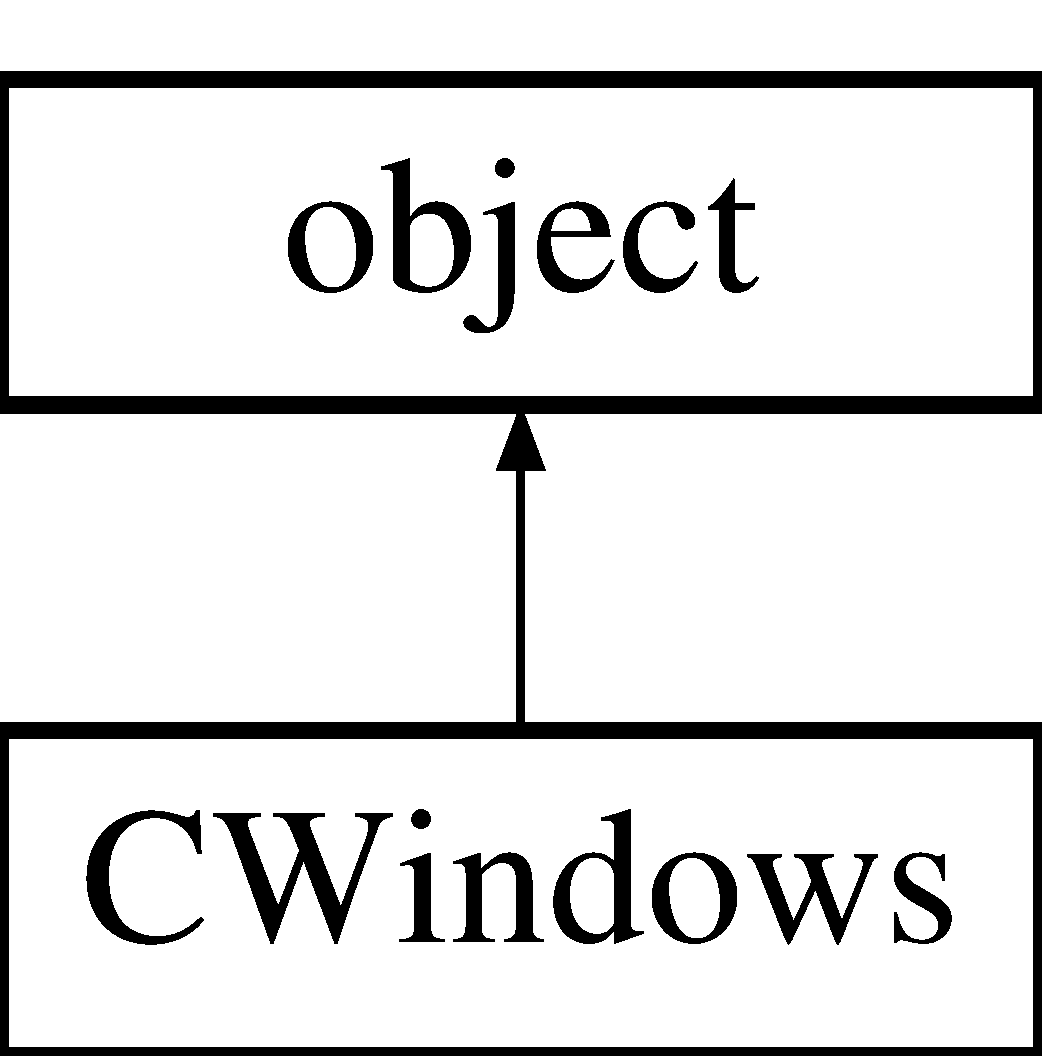
\includegraphics[height=2.000000cm]{class_c_windows_1_1_c_windows}
\end{center}
\end{figure}
\subsection*{Public Member Functions}
\begin{DoxyCompactItemize}
\item 
\mbox{\Hypertarget{class_c_windows_1_1_c_windows_abbcfc1a774079da020e49c42cbadb693}\label{class_c_windows_1_1_c_windows_abbcfc1a774079da020e49c42cbadb693}} 
def {\bfseries U\+U\+ID} (self)
\item 
\mbox{\Hypertarget{class_c_windows_1_1_c_windows_aff464267544e4efc9b770c8320c8f199}\label{class_c_windows_1_1_c_windows_aff464267544e4efc9b770c8320c8f199}} 
def {\bfseries type} (self)
\item 
\mbox{\Hypertarget{class_c_windows_1_1_c_windows_aca033702f187894894d3102de41d6b99}\label{class_c_windows_1_1_c_windows_aca033702f187894894d3102de41d6b99}} 
def {\bfseries type} (self, value)
\item 
\mbox{\Hypertarget{class_c_windows_1_1_c_windows_adb8818239148d2e5c5833a2b062ee9ad}\label{class_c_windows_1_1_c_windows_adb8818239148d2e5c5833a2b062ee9ad}} 
def {\bfseries ID} (self)
\item 
\mbox{\Hypertarget{class_c_windows_1_1_c_windows_a0a178fbcae3f6431733dd63ee37ac7bb}\label{class_c_windows_1_1_c_windows_a0a178fbcae3f6431733dd63ee37ac7bb}} 
def {\bfseries ID} (self, value)
\item 
\mbox{\Hypertarget{class_c_windows_1_1_c_windows_a05cd4cd28b324f262fefe1a1782bd992}\label{class_c_windows_1_1_c_windows_a05cd4cd28b324f262fefe1a1782bd992}} 
def {\bfseries enabled} (self)
\item 
\mbox{\Hypertarget{class_c_windows_1_1_c_windows_a18495e0c3f2639c84751c9aa77cd03b3}\label{class_c_windows_1_1_c_windows_a18495e0c3f2639c84751c9aa77cd03b3}} 
def {\bfseries enabled} (self, value)
\item 
\mbox{\Hypertarget{class_c_windows_1_1_c_windows_a71963b9940a29bf3f2c10546c2cb9b50}\label{class_c_windows_1_1_c_windows_a71963b9940a29bf3f2c10546c2cb9b50}} 
def {\bfseries \+\_\+\+\_\+init\+\_\+\+\_\+} (self, id=str(uuid.\+uuid4()), enabled=True)
\end{DoxyCompactItemize}


\subsection{Detailed Description}


Definition at line 12 of file C\+Windows.\+py.



The documentation for this class was generated from the following file\+:\begin{DoxyCompactItemize}
\item 
C\+Windows.\+py\end{DoxyCompactItemize}

\hypertarget{class_c_zone_1_1_c_zone}{}\section{C\+Zone Class Reference}
\label{class_c_zone_1_1_c_zone}\index{C\+Zone@{C\+Zone}}
Inheritance diagram for C\+Zone\+:\begin{figure}[H]
\begin{center}
\leavevmode
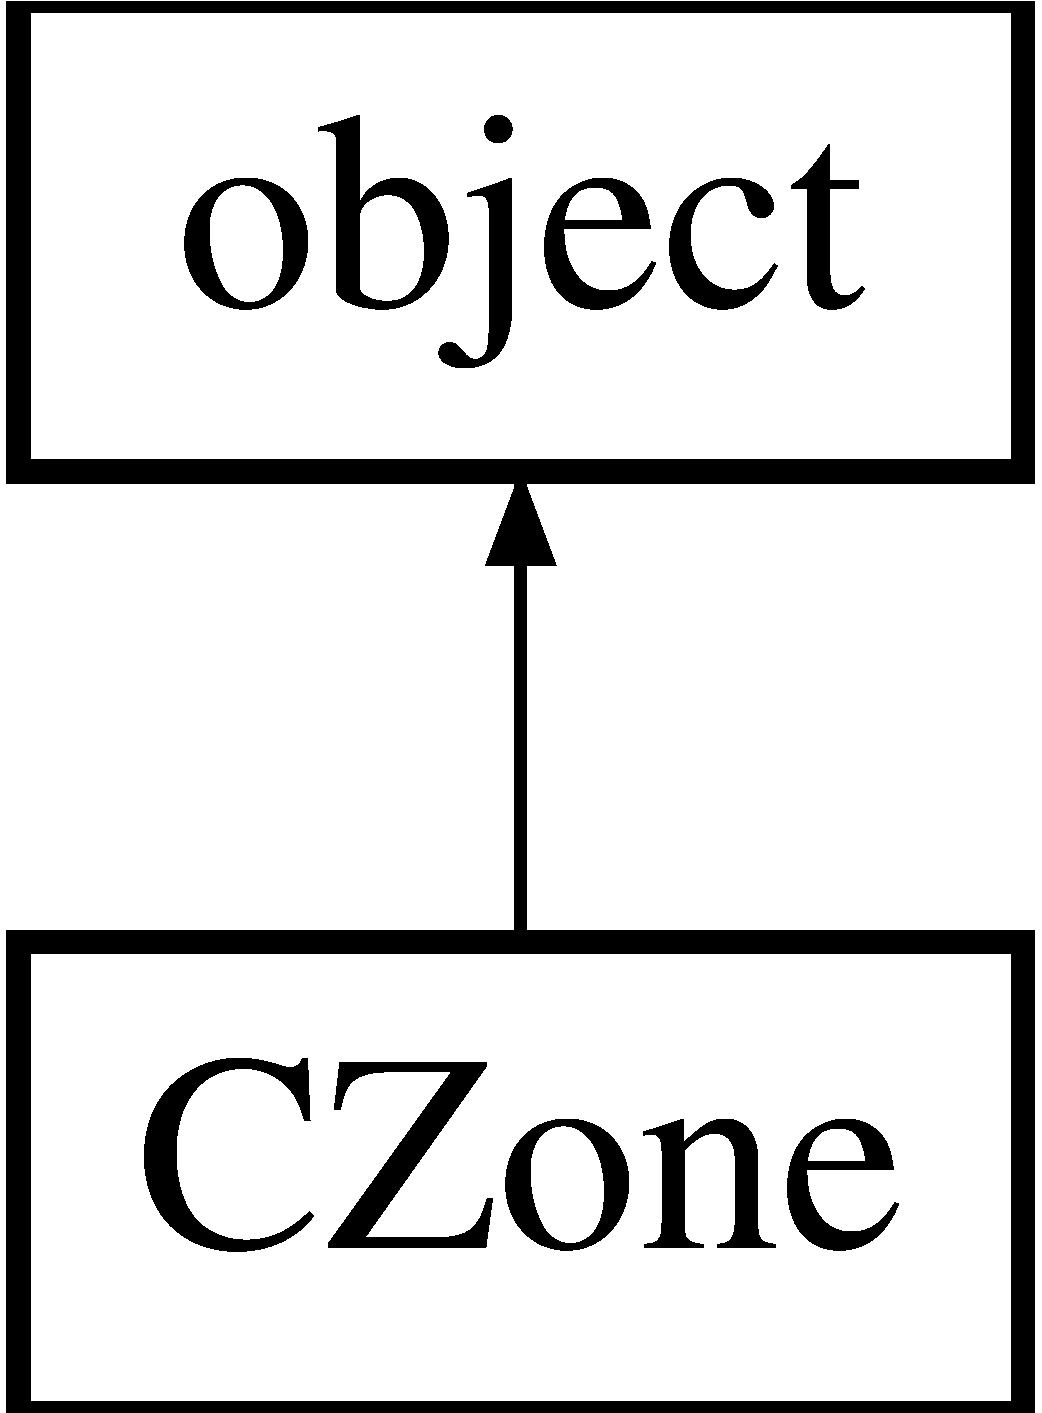
\includegraphics[height=2.000000cm]{class_c_zone_1_1_c_zone}
\end{center}
\end{figure}
\subsection*{Public Member Functions}
\begin{DoxyCompactItemize}
\item 
\mbox{\Hypertarget{class_c_zone_1_1_c_zone_abbcfc1a774079da020e49c42cbadb693}\label{class_c_zone_1_1_c_zone_abbcfc1a774079da020e49c42cbadb693}} 
def {\bfseries U\+U\+ID} (self)
\item 
\mbox{\Hypertarget{class_c_zone_1_1_c_zone_aff464267544e4efc9b770c8320c8f199}\label{class_c_zone_1_1_c_zone_aff464267544e4efc9b770c8320c8f199}} 
def {\bfseries type} (self)
\item 
\mbox{\Hypertarget{class_c_zone_1_1_c_zone_aca033702f187894894d3102de41d6b99}\label{class_c_zone_1_1_c_zone_aca033702f187894894d3102de41d6b99}} 
def {\bfseries type} (self, value)
\item 
\mbox{\Hypertarget{class_c_zone_1_1_c_zone_adb8818239148d2e5c5833a2b062ee9ad}\label{class_c_zone_1_1_c_zone_adb8818239148d2e5c5833a2b062ee9ad}} 
def {\bfseries ID} (self)
\item 
\mbox{\Hypertarget{class_c_zone_1_1_c_zone_a0a178fbcae3f6431733dd63ee37ac7bb}\label{class_c_zone_1_1_c_zone_a0a178fbcae3f6431733dd63ee37ac7bb}} 
def {\bfseries ID} (self, value)
\item 
\mbox{\Hypertarget{class_c_zone_1_1_c_zone_a5907ca3bbf8e7cd8f40c3007338f6d02}\label{class_c_zone_1_1_c_zone_a5907ca3bbf8e7cd8f40c3007338f6d02}} 
def {\bfseries name} (self)
\item 
\mbox{\Hypertarget{class_c_zone_1_1_c_zone_a62d212fdcbbcee30e90a64ce349d32f8}\label{class_c_zone_1_1_c_zone_a62d212fdcbbcee30e90a64ce349d32f8}} 
def {\bfseries name} (self, value)
\item 
\mbox{\Hypertarget{class_c_zone_1_1_c_zone_ae74a168e4a0b35119d7e38ba6fa12fd7}\label{class_c_zone_1_1_c_zone_ae74a168e4a0b35119d7e38ba6fa12fd7}} 
def {\bfseries activities} (self)
\item 
\mbox{\Hypertarget{class_c_zone_1_1_c_zone_ace542f219ac250dd15be04c2a610f031}\label{class_c_zone_1_1_c_zone_ace542f219ac250dd15be04c2a610f031}} 
def {\bfseries activities} (self, value)
\item 
\mbox{\Hypertarget{class_c_zone_1_1_c_zone_a9d0a5ea0a19a2297c8c9947ba979c976}\label{class_c_zone_1_1_c_zone_a9d0a5ea0a19a2297c8c9947ba979c976}} 
def {\bfseries ground\+Floor} (self)
\item 
\mbox{\Hypertarget{class_c_zone_1_1_c_zone_af46a0905d14fd5a6d6da9689d4f02b4c}\label{class_c_zone_1_1_c_zone_af46a0905d14fd5a6d6da9689d4f02b4c}} 
def {\bfseries ground\+Floor} (self, value)
\item 
\mbox{\Hypertarget{class_c_zone_1_1_c_zone_aa42303929133897776f13907e0431c0f}\label{class_c_zone_1_1_c_zone_aa42303929133897776f13907e0431c0f}} 
def {\bfseries window\+Count} (self)
\item 
\mbox{\Hypertarget{class_c_zone_1_1_c_zone_af3677ddf979f1265c118cfc443f1d331}\label{class_c_zone_1_1_c_zone_af3677ddf979f1265c118cfc443f1d331}} 
def {\bfseries window\+Count} (self, value)
\item 
\mbox{\Hypertarget{class_c_zone_1_1_c_zone_abdc78e81ef4a07ee7ba9793bbf69af2c}\label{class_c_zone_1_1_c_zone_abdc78e81ef4a07ee7ba9793bbf69af2c}} 
def {\bfseries floor\+Area} (self)
\item 
\mbox{\Hypertarget{class_c_zone_1_1_c_zone_a576ae6723af0e4ea4336b50a2e6e2aaf}\label{class_c_zone_1_1_c_zone_a576ae6723af0e4ea4336b50a2e6e2aaf}} 
def {\bfseries floor\+Area} (self, value)
\item 
\mbox{\Hypertarget{class_c_zone_1_1_c_zone_acd55f81742453744a48338238ae1d0e2}\label{class_c_zone_1_1_c_zone_acd55f81742453744a48338238ae1d0e2}} 
def {\bfseries \+\_\+\+\_\+init\+\_\+\+\_\+} (self, id=str(uuid.\+uuid4()), name=\textquotesingle{}\textquotesingle{}, activities=\textquotesingle{}\textquotesingle{}, ground\+Floor=False, window\+Count=0, floor\+Area=0)
\end{DoxyCompactItemize}


\subsection{Detailed Description}


Definition at line 12 of file C\+Zone.\+py.



The documentation for this class was generated from the following file\+:\begin{DoxyCompactItemize}
\item 
C\+Zone.\+py\end{DoxyCompactItemize}

\hypertarget{class_c_utils_1_1_utils_1_1_u_i_1_1_controls_1_1_drop_down_list}{}\section{Utils.\+U\+I.\+Controls.\+Drop\+Down\+List Class Reference}
\label{class_c_utils_1_1_utils_1_1_u_i_1_1_controls_1_1_drop_down_list}\index{Utils.\+U\+I.\+Controls.\+Drop\+Down\+List@{Utils.\+U\+I.\+Controls.\+Drop\+Down\+List}}
Inheritance diagram for Utils.\+U\+I.\+Controls.\+Drop\+Down\+List\+:\begin{figure}[H]
\begin{center}
\leavevmode
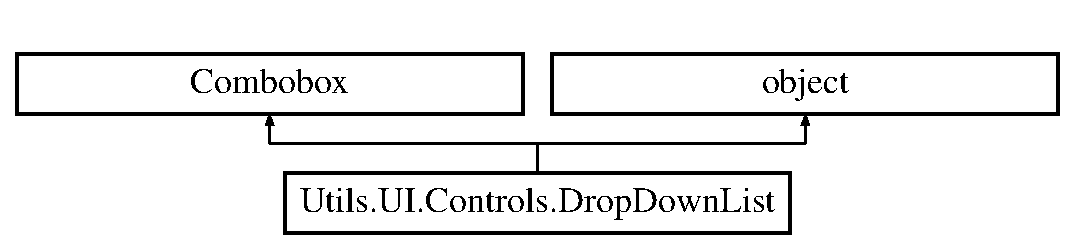
\includegraphics[height=2.000000cm]{class_c_utils_1_1_utils_1_1_u_i_1_1_controls_1_1_drop_down_list}
\end{center}
\end{figure}
\subsection*{Public Member Functions}
\begin{DoxyCompactItemize}
\item 
\mbox{\Hypertarget{class_c_utils_1_1_utils_1_1_u_i_1_1_controls_1_1_drop_down_list_a9d7a16fcda2089f0b7f1142f6bf45acd}\label{class_c_utils_1_1_utils_1_1_u_i_1_1_controls_1_1_drop_down_list_a9d7a16fcda2089f0b7f1142f6bf45acd}} 
def {\bfseries On\+Selected\+Index\+Changed} (self, event=None)
\item 
\mbox{\Hypertarget{class_c_utils_1_1_utils_1_1_u_i_1_1_controls_1_1_drop_down_list_a5b0816a06a090d1fa84ff907f1b072ba}\label{class_c_utils_1_1_utils_1_1_u_i_1_1_controls_1_1_drop_down_list_a5b0816a06a090d1fa84ff907f1b072ba}} 
def {\bfseries set\+Variable} (self, ref\+Text\+Variable)
\item 
\mbox{\Hypertarget{class_c_utils_1_1_utils_1_1_u_i_1_1_controls_1_1_drop_down_list_aa26b36a4ffc32d15799ee486097fe330}\label{class_c_utils_1_1_utils_1_1_u_i_1_1_controls_1_1_drop_down_list_aa26b36a4ffc32d15799ee486097fe330}} 
def {\bfseries set\+Variables} (self, ref\+Key\+Variable, ref\+Text\+Variable)
\item 
\mbox{\Hypertarget{class_c_utils_1_1_utils_1_1_u_i_1_1_controls_1_1_drop_down_list_af77a3768a0873465ab21261595c09d38}\label{class_c_utils_1_1_utils_1_1_u_i_1_1_controls_1_1_drop_down_list_af77a3768a0873465ab21261595c09d38}} 
def {\bfseries get\+Element\+By\+Text} (self, text\+Value)
\item 
\mbox{\Hypertarget{class_c_utils_1_1_utils_1_1_u_i_1_1_controls_1_1_drop_down_list_a3ed216411c7b741af5d86d493850f9fb}\label{class_c_utils_1_1_utils_1_1_u_i_1_1_controls_1_1_drop_down_list_a3ed216411c7b741af5d86d493850f9fb}} 
def {\bfseries reset\+Selection} (self)
\item 
\mbox{\Hypertarget{class_c_utils_1_1_utils_1_1_u_i_1_1_controls_1_1_drop_down_list_a2d9f1b9bed847ff75b9f232ced637286}\label{class_c_utils_1_1_utils_1_1_u_i_1_1_controls_1_1_drop_down_list_a2d9f1b9bed847ff75b9f232ced637286}} 
def {\bfseries \+\_\+\+\_\+init\+\_\+\+\_\+} (self, parent, args, kwargs)
\end{DoxyCompactItemize}


\subsection{Detailed Description}


Definition at line 342 of file C\+Utils.\+py.



The documentation for this class was generated from the following file\+:\begin{DoxyCompactItemize}
\item 
C\+Utils.\+py\end{DoxyCompactItemize}

\hypertarget{class_f_building_1_1_frm_building}{}\section{Frm\+Building Class Reference}
\label{class_f_building_1_1_frm_building}\index{Frm\+Building@{Frm\+Building}}
Inheritance diagram for Frm\+Building\+:\begin{figure}[H]
\begin{center}
\leavevmode
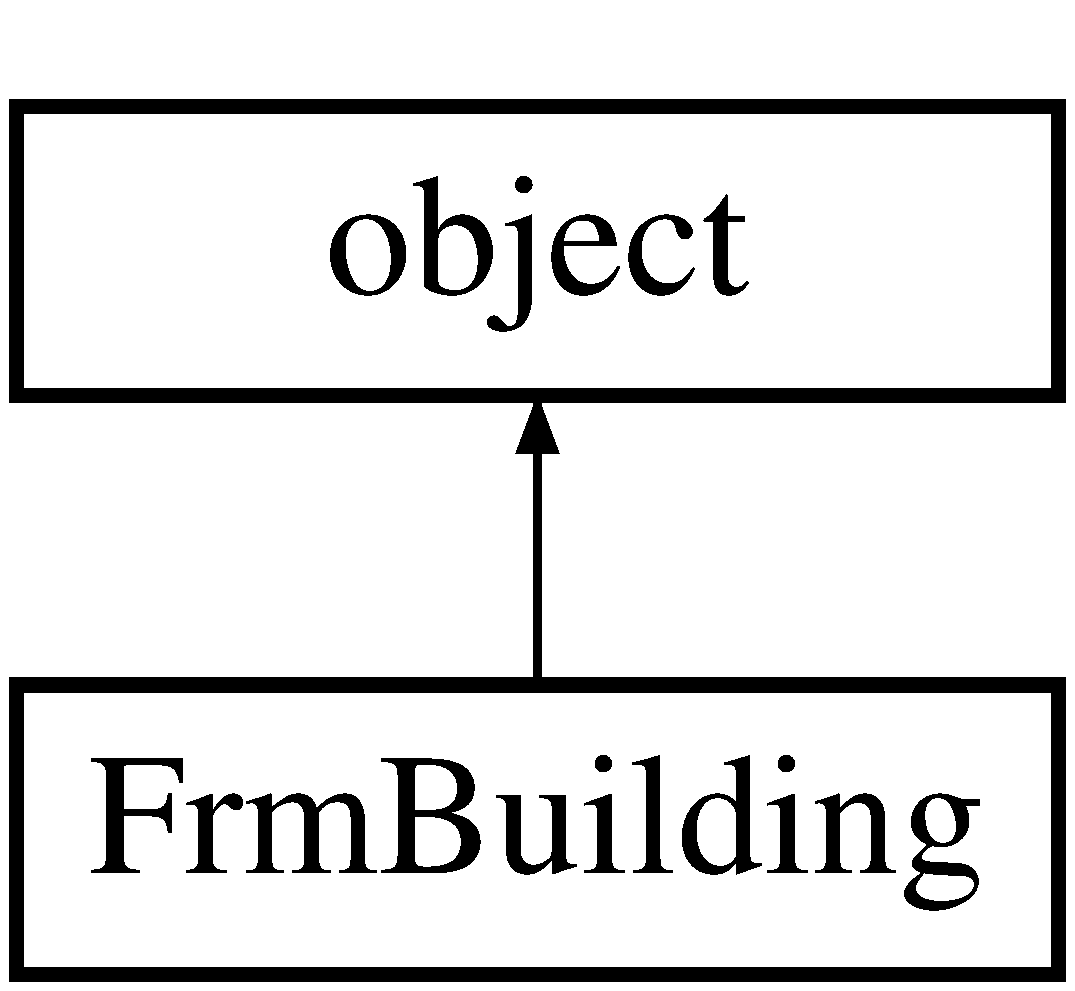
\includegraphics[height=2.000000cm]{class_f_building_1_1_frm_building}
\end{center}
\end{figure}
\subsection*{Public Member Functions}
\begin{DoxyCompactItemize}
\item 
\mbox{\Hypertarget{class_f_building_1_1_frm_building_a72f6c394e1999939f9d9b5580c86dcc2}\label{class_f_building_1_1_frm_building_a72f6c394e1999939f9d9b5580c86dcc2}} 
def {\bfseries load} (self, id=None, name=None, show=False)
\item 
\mbox{\Hypertarget{class_f_building_1_1_frm_building_ab4f4398c3f210fe4ea6e720401357691}\label{class_f_building_1_1_frm_building_ab4f4398c3f210fe4ea6e720401357691}} 
def {\bfseries show} (self)
\item 
\mbox{\Hypertarget{class_f_building_1_1_frm_building_a9ad70aa10f26bd59d99d7abb5abb7565}\label{class_f_building_1_1_frm_building_a9ad70aa10f26bd59d99d7abb5abb7565}} 
def {\bfseries \+\_\+\+\_\+init\+\_\+\+\_\+} (self, master, parent, id=0, name=\textquotesingle{}\textquotesingle{})
\end{DoxyCompactItemize}
\subsection*{Public Attributes}
\begin{DoxyCompactItemize}
\item 
\mbox{\Hypertarget{class_f_building_1_1_frm_building_afe9b98e5038ae1c69e5bb7eef0ed7cc4}\label{class_f_building_1_1_frm_building_afe9b98e5038ae1c69e5bb7eef0ed7cc4}} 
{\bfseries lblname}
\item 
\mbox{\Hypertarget{class_f_building_1_1_frm_building_a24025fc9f698a9db8fb4f3c1c3c32e40}\label{class_f_building_1_1_frm_building_a24025fc9f698a9db8fb4f3c1c3c32e40}} 
{\bfseries txtname}
\end{DoxyCompactItemize}


\subsection{Detailed Description}


Definition at line 14 of file F\+Building.\+py.



The documentation for this class was generated from the following file\+:\begin{DoxyCompactItemize}
\item 
F\+Building.\+py\end{DoxyCompactItemize}

\hypertarget{class_f_configuration_1_1_frm_configuration}{}\section{Frm\+Configuration Class Reference}
\label{class_f_configuration_1_1_frm_configuration}\index{Frm\+Configuration@{Frm\+Configuration}}
Inheritance diagram for Frm\+Configuration\+:\begin{figure}[H]
\begin{center}
\leavevmode
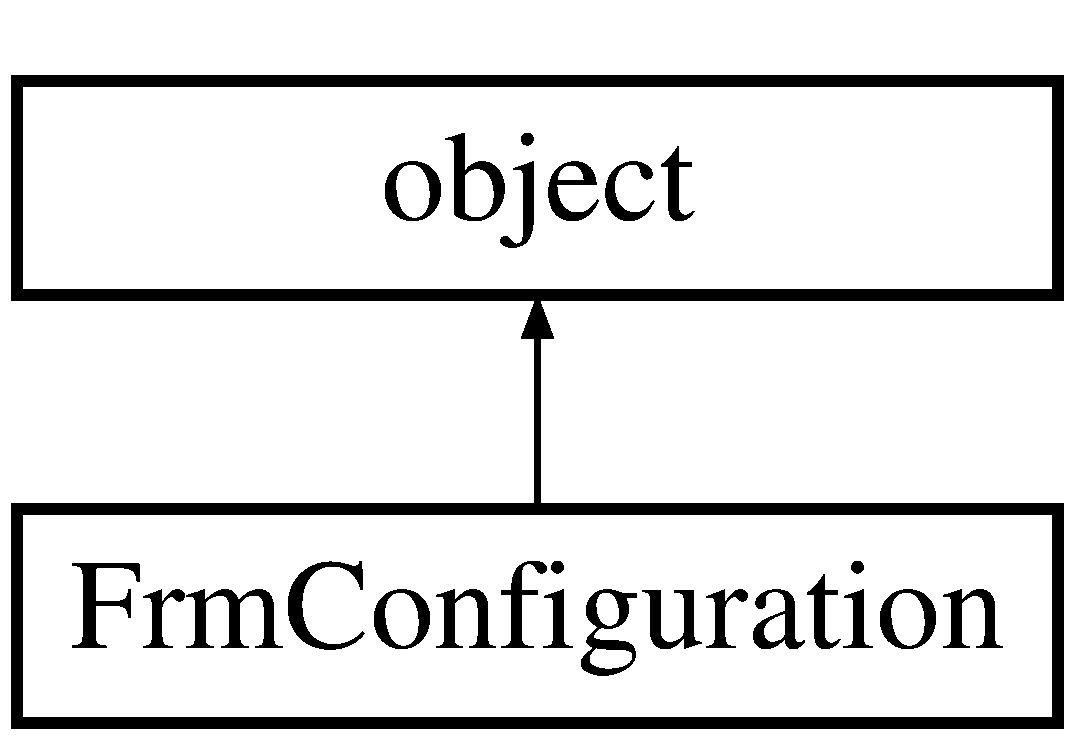
\includegraphics[height=2.000000cm]{class_f_configuration_1_1_frm_configuration}
\end{center}
\end{figure}
\subsection*{Public Member Functions}
\begin{DoxyCompactItemize}
\item 
\mbox{\Hypertarget{class_f_configuration_1_1_frm_configuration_adb8818239148d2e5c5833a2b062ee9ad}\label{class_f_configuration_1_1_frm_configuration_adb8818239148d2e5c5833a2b062ee9ad}} 
def {\bfseries ID} (self)
\item 
\mbox{\Hypertarget{class_f_configuration_1_1_frm_configuration_acf44064249ee17c3e8952b4c33512f86}\label{class_f_configuration_1_1_frm_configuration_acf44064249ee17c3e8952b4c33512f86}} 
def {\bfseries Frame} (self)
\item 
\mbox{\Hypertarget{class_f_configuration_1_1_frm_configuration_a3631deb3926b738843f8dd6e69fbd259}\label{class_f_configuration_1_1_frm_configuration_a3631deb3926b738843f8dd6e69fbd259}} 
def {\bfseries type\+Of\+Building} (self)
\item 
\mbox{\Hypertarget{class_f_configuration_1_1_frm_configuration_a3a6c08954737f19a6d16a22e25125641}\label{class_f_configuration_1_1_frm_configuration_a3a6c08954737f19a6d16a22e25125641}} 
def {\bfseries area} (self)
\item 
\mbox{\Hypertarget{class_f_configuration_1_1_frm_configuration_ab88765a5be3931ab35880d4a76f4c6e0}\label{class_f_configuration_1_1_frm_configuration_ab88765a5be3931ab35880d4a76f4c6e0}} 
def {\bfseries number\+Of\+Occupants} (self)
\item 
\mbox{\Hypertarget{class_f_configuration_1_1_frm_configuration_a3635a14f0ea9fe8467061d980596ad22}\label{class_f_configuration_1_1_frm_configuration_a3635a14f0ea9fe8467061d980596ad22}} 
def {\bfseries seed} (self)
\item 
\mbox{\Hypertarget{class_f_configuration_1_1_frm_configuration_af286205505c104c81c0242d14a95bb12}\label{class_f_configuration_1_1_frm_configuration_af286205505c104c81c0242d14a95bb12}} 
def {\bfseries time\+Steps\+Per\+Hour} (self)
\item 
\mbox{\Hypertarget{class_f_configuration_1_1_frm_configuration_a6c7372cee655ba961184c4fe96a8bd5f}\label{class_f_configuration_1_1_frm_configuration_a6c7372cee655ba961184c4fe96a8bd5f}} 
def {\bfseries begin\+Month} (self)
\item 
\mbox{\Hypertarget{class_f_configuration_1_1_frm_configuration_afad533b6229d7962cdcb6a1967e12624}\label{class_f_configuration_1_1_frm_configuration_afad533b6229d7962cdcb6a1967e12624}} 
def {\bfseries end\+Month} (self)
\item 
\mbox{\Hypertarget{class_f_configuration_1_1_frm_configuration_ad7ed6684dccd3d75d5aac2fa8717ec3d}\label{class_f_configuration_1_1_frm_configuration_ad7ed6684dccd3d75d5aac2fa8717ec3d}} 
def {\bfseries begin\+Day} (self)
\item 
\mbox{\Hypertarget{class_f_configuration_1_1_frm_configuration_a80d8125dbc72366ec74279237dce91f5}\label{class_f_configuration_1_1_frm_configuration_a80d8125dbc72366ec74279237dce91f5}} 
def {\bfseries end\+Day} (self)
\item 
\mbox{\Hypertarget{class_f_configuration_1_1_frm_configuration_a00302b53a9e68912d194f05f103164a1}\label{class_f_configuration_1_1_frm_configuration_a00302b53a9e68912d194f05f103164a1}} 
def {\bfseries learn} (self)
\item 
\mbox{\Hypertarget{class_f_configuration_1_1_frm_configuration_a564562f082521e37c7029e239abb56c6}\label{class_f_configuration_1_1_frm_configuration_a564562f082521e37c7029e239abb56c6}} 
def {\bfseries save} (self)
\item 
\mbox{\Hypertarget{class_f_configuration_1_1_frm_configuration_a84c26bac805a51ec23a04b7da2d22a51}\label{class_f_configuration_1_1_frm_configuration_a84c26bac805a51ec23a04b7da2d22a51}} 
def {\bfseries eplus\+Version} (self)
\item 
\mbox{\Hypertarget{class_f_configuration_1_1_frm_configuration_adf514cfb8e3643353b281dc14f9ce3b1}\label{class_f_configuration_1_1_frm_configuration_adf514cfb8e3643353b281dc14f9ce3b1}} 
def {\bfseries number\+Of\+Replicates} (self)
\item 
\mbox{\Hypertarget{class_f_configuration_1_1_frm_configuration_a309c3e506f9b70284537fca739ecdafb}\label{class_f_configuration_1_1_frm_configuration_a309c3e506f9b70284537fca739ecdafb}} 
def {\bfseries number\+Of\+Replicates\+Random} (self)
\item 
\mbox{\Hypertarget{class_f_configuration_1_1_frm_configuration_a40757e196682a19b112ac3d015fc6948}\label{class_f_configuration_1_1_frm_configuration_a40757e196682a19b112ac3d015fc6948}} 
def {\bfseries load\+Obj\+Simulation} (self, obj\+Simulation)
\item 
\mbox{\Hypertarget{class_f_configuration_1_1_frm_configuration_a1f1d7472c755120a61441b70e668ee75}\label{class_f_configuration_1_1_frm_configuration_a1f1d7472c755120a61441b70e668ee75}} 
def {\bfseries \+\_\+\+\_\+init\+\_\+\+\_\+} (self, parent, obj\+Simulation)
\end{DoxyCompactItemize}
\subsection*{Public Attributes}
\begin{DoxyCompactItemize}
\item 
\mbox{\Hypertarget{class_f_configuration_1_1_frm_configuration_a61ad0bc14892769644b9814451324013}\label{class_f_configuration_1_1_frm_configuration_a61ad0bc14892769644b9814451324013}} 
{\bfseries ddl\+Type\+Of\+Building}
\item 
\mbox{\Hypertarget{class_f_configuration_1_1_frm_configuration_a67725d9f5fa5e74e8a5243581232ff0d}\label{class_f_configuration_1_1_frm_configuration_a67725d9f5fa5e74e8a5243581232ff0d}} 
{\bfseries txt\+Area}
\item 
\mbox{\Hypertarget{class_f_configuration_1_1_frm_configuration_a06615eb4db15a80863045eb57b31f74e}\label{class_f_configuration_1_1_frm_configuration_a06615eb4db15a80863045eb57b31f74e}} 
{\bfseries txt\+Number\+Occupants}
\item 
\mbox{\Hypertarget{class_f_configuration_1_1_frm_configuration_a858b46cdd4389be09bbb861529c12311}\label{class_f_configuration_1_1_frm_configuration_a858b46cdd4389be09bbb861529c12311}} 
{\bfseries txt\+Seed}
\item 
\mbox{\Hypertarget{class_f_configuration_1_1_frm_configuration_a2313924898b624c24476936cbb9c9e78}\label{class_f_configuration_1_1_frm_configuration_a2313924898b624c24476936cbb9c9e78}} 
{\bfseries txt\+Time\+Steps\+P\+Hour}
\item 
\mbox{\Hypertarget{class_f_configuration_1_1_frm_configuration_ad1af6d226165104a1e8ebccdd7263078}\label{class_f_configuration_1_1_frm_configuration_ad1af6d226165104a1e8ebccdd7263078}} 
{\bfseries txt\+Begin\+Month}
\item 
\mbox{\Hypertarget{class_f_configuration_1_1_frm_configuration_a535534b01b15b9cf2c3f83f1f13ee89e}\label{class_f_configuration_1_1_frm_configuration_a535534b01b15b9cf2c3f83f1f13ee89e}} 
{\bfseries txt\+End\+Month}
\item 
\mbox{\Hypertarget{class_f_configuration_1_1_frm_configuration_a93be85acd3b240065aa600416ab3de17}\label{class_f_configuration_1_1_frm_configuration_a93be85acd3b240065aa600416ab3de17}} 
{\bfseries txt\+Begin\+Day}
\item 
\mbox{\Hypertarget{class_f_configuration_1_1_frm_configuration_ac979d2725ba1bcfd0e0d8ca272d99dfb}\label{class_f_configuration_1_1_frm_configuration_ac979d2725ba1bcfd0e0d8ca272d99dfb}} 
{\bfseries txt\+End\+Day}
\item 
\mbox{\Hypertarget{class_f_configuration_1_1_frm_configuration_ae413b6d8d9c45f1720715a7b2542df1d}\label{class_f_configuration_1_1_frm_configuration_ae413b6d8d9c45f1720715a7b2542df1d}} 
{\bfseries chk\+Learn}
\item 
\mbox{\Hypertarget{class_f_configuration_1_1_frm_configuration_a9a9e8283eef05e484fde00282079f7f3}\label{class_f_configuration_1_1_frm_configuration_a9a9e8283eef05e484fde00282079f7f3}} 
{\bfseries chk\+Save}
\item 
\mbox{\Hypertarget{class_f_configuration_1_1_frm_configuration_a8eea02931fed24e1f07bda5d78b288a2}\label{class_f_configuration_1_1_frm_configuration_a8eea02931fed24e1f07bda5d78b288a2}} 
{\bfseries ddl\+E\+Plus\+Version}
\item 
\mbox{\Hypertarget{class_f_configuration_1_1_frm_configuration_a355d26c83acdd67f5885f477d030e417}\label{class_f_configuration_1_1_frm_configuration_a355d26c83acdd67f5885f477d030e417}} 
{\bfseries txt\+Number\+Replicates}
\item 
\mbox{\Hypertarget{class_f_configuration_1_1_frm_configuration_a0738497e1097dbcec26eaa7a1d84d507}\label{class_f_configuration_1_1_frm_configuration_a0738497e1097dbcec26eaa7a1d84d507}} 
{\bfseries txt\+Number\+Replicates\+Random}
\end{DoxyCompactItemize}


\subsection{Detailed Description}


Definition at line 14 of file F\+Configuration.\+py.



The documentation for this class was generated from the following file\+:\begin{DoxyCompactItemize}
\item 
F\+Configuration.\+py\end{DoxyCompactItemize}

\hypertarget{class_f_empty_1_1_frm_empty}{}\section{Frm\+Empty Class Reference}
\label{class_f_empty_1_1_frm_empty}\index{Frm\+Empty@{Frm\+Empty}}
Inheritance diagram for Frm\+Empty\+:\begin{figure}[H]
\begin{center}
\leavevmode
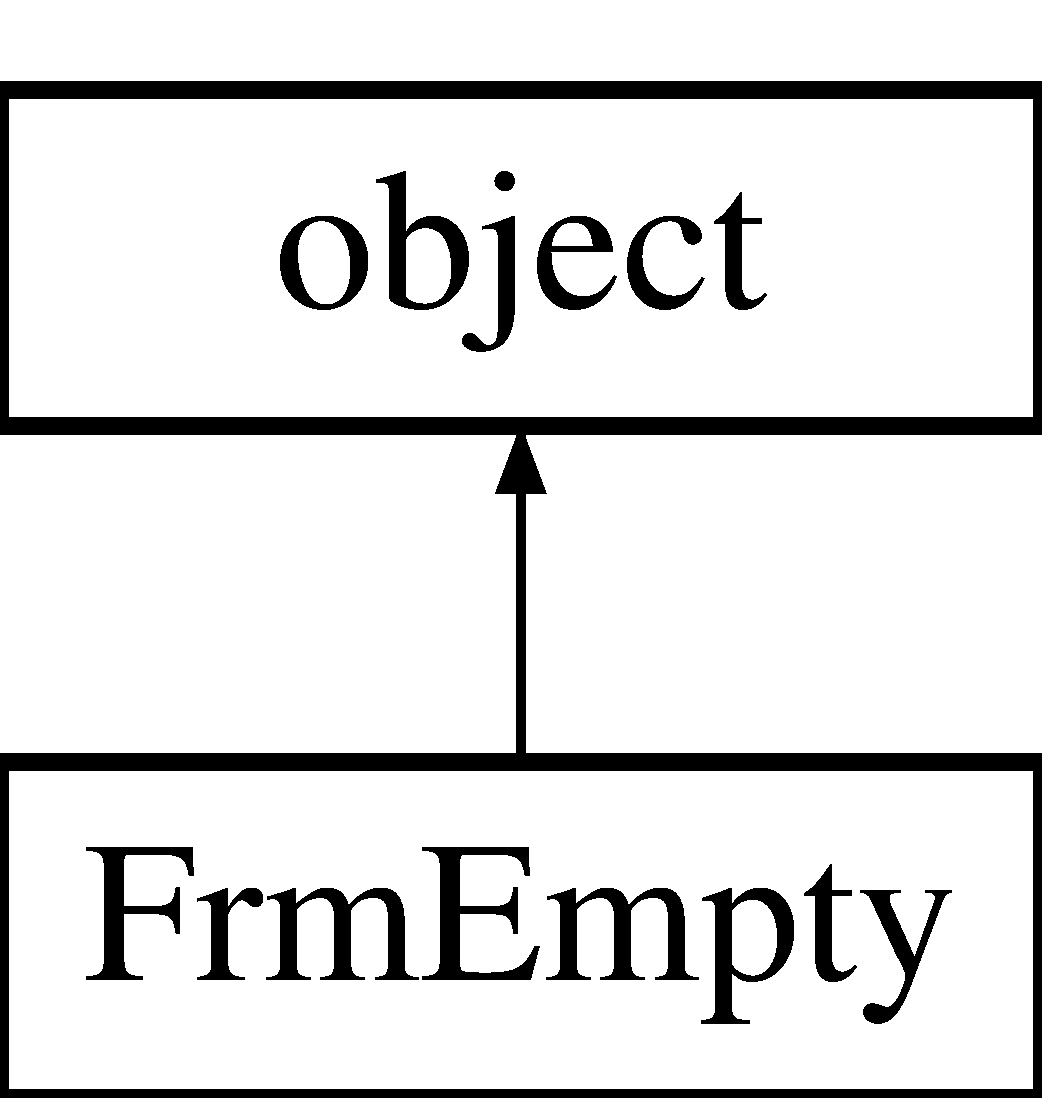
\includegraphics[height=2.000000cm]{class_f_empty_1_1_frm_empty}
\end{center}
\end{figure}
\subsection*{Public Member Functions}
\begin{DoxyCompactItemize}
\item 
\mbox{\Hypertarget{class_f_empty_1_1_frm_empty_adb8818239148d2e5c5833a2b062ee9ad}\label{class_f_empty_1_1_frm_empty_adb8818239148d2e5c5833a2b062ee9ad}} 
def {\bfseries ID} (self)
\item 
\mbox{\Hypertarget{class_f_empty_1_1_frm_empty_acf44064249ee17c3e8952b4c33512f86}\label{class_f_empty_1_1_frm_empty_acf44064249ee17c3e8952b4c33512f86}} 
def {\bfseries Frame} (self)
\item 
\mbox{\Hypertarget{class_f_empty_1_1_frm_empty_ab83ff91f3f9776b4af9b931631e73091}\label{class_f_empty_1_1_frm_empty_ab83ff91f3f9776b4af9b931631e73091}} 
def {\bfseries load} (self, title=None)
\item 
\mbox{\Hypertarget{class_f_empty_1_1_frm_empty_ab4f4398c3f210fe4ea6e720401357691}\label{class_f_empty_1_1_frm_empty_ab4f4398c3f210fe4ea6e720401357691}} 
def {\bfseries show} (self)
\item 
\mbox{\Hypertarget{class_f_empty_1_1_frm_empty_a955a7cdca50525c17f86368cb44b1039}\label{class_f_empty_1_1_frm_empty_a955a7cdca50525c17f86368cb44b1039}} 
def {\bfseries title} (self)
\item 
\mbox{\Hypertarget{class_f_empty_1_1_frm_empty_a9e6a9fff264031ba43ff34c096154972}\label{class_f_empty_1_1_frm_empty_a9e6a9fff264031ba43ff34c096154972}} 
def {\bfseries title} (self, value)
\item 
\mbox{\Hypertarget{class_f_empty_1_1_frm_empty_a75020e7f3888d6f837fae592b305add8}\label{class_f_empty_1_1_frm_empty_a75020e7f3888d6f837fae592b305add8}} 
def {\bfseries \+\_\+\+\_\+init\+\_\+\+\_\+} (self, parent)
\end{DoxyCompactItemize}


\subsection{Detailed Description}


Definition at line 12 of file F\+Empty.\+py.



The documentation for this class was generated from the following file\+:\begin{DoxyCompactItemize}
\item 
F\+Empty.\+py\end{DoxyCompactItemize}

\hypertarget{class_f_lights_1_1_frm_lights}{}\section{Frm\+Lights Class Reference}
\label{class_f_lights_1_1_frm_lights}\index{Frm\+Lights@{Frm\+Lights}}
Inheritance diagram for Frm\+Lights\+:\begin{figure}[H]
\begin{center}
\leavevmode
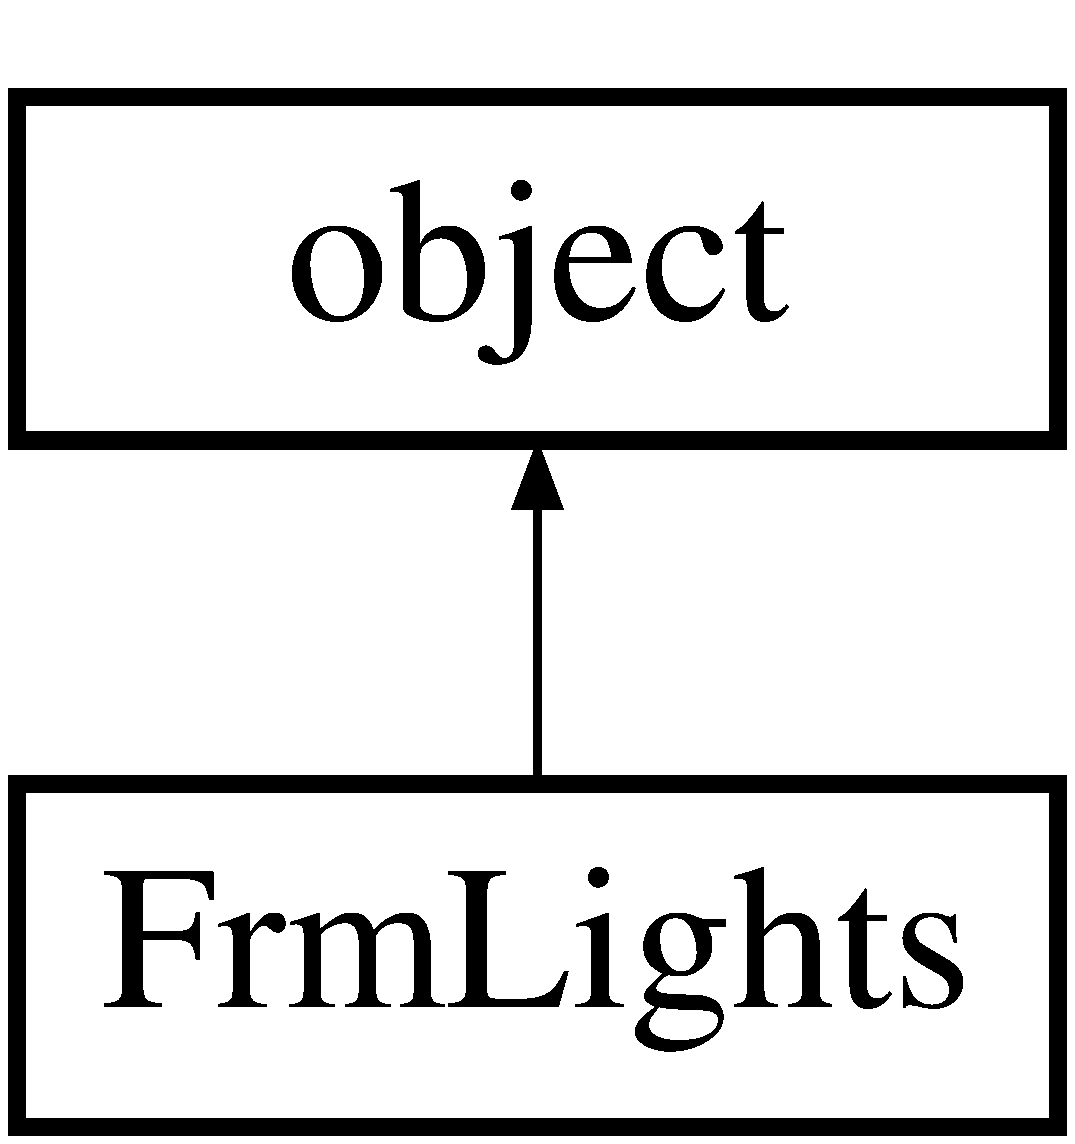
\includegraphics[height=2.000000cm]{class_f_lights_1_1_frm_lights}
\end{center}
\end{figure}
\subsection*{Public Member Functions}
\begin{DoxyCompactItemize}
\item 
\mbox{\Hypertarget{class_f_lights_1_1_frm_lights_a38f4c0a1b0b9f14e89e7670d417e140a}\label{class_f_lights_1_1_frm_lights_a38f4c0a1b0b9f14e89e7670d417e140a}} 
def {\bfseries load} (self, var\+Enabled, show=False)
\item 
\mbox{\Hypertarget{class_f_lights_1_1_frm_lights_ab4f4398c3f210fe4ea6e720401357691}\label{class_f_lights_1_1_frm_lights_ab4f4398c3f210fe4ea6e720401357691}} 
def {\bfseries show} (self)
\item 
\mbox{\Hypertarget{class_f_lights_1_1_frm_lights_adffadd9833af4759460d71b7d00bbf4c}\label{class_f_lights_1_1_frm_lights_adffadd9833af4759460d71b7d00bbf4c}} 
def {\bfseries \+\_\+\+\_\+init\+\_\+\+\_\+} (self, master, parent, enabled=False)
\end{DoxyCompactItemize}
\subsection*{Public Attributes}
\begin{DoxyCompactItemize}
\item 
\mbox{\Hypertarget{class_f_lights_1_1_frm_lights_aa5ba96b8972782a03e3d83def0f965a9}\label{class_f_lights_1_1_frm_lights_aa5ba96b8972782a03e3d83def0f965a9}} 
{\bfseries chk\+Enabled}
\end{DoxyCompactItemize}


\subsection{Detailed Description}


Definition at line 14 of file F\+Lights.\+py.



The documentation for this class was generated from the following file\+:\begin{DoxyCompactItemize}
\item 
F\+Lights.\+py\end{DoxyCompactItemize}

\hypertarget{class_f_list_of_zones_verification_1_1_frm_list_of_zones_verification}{}\section{Frm\+List\+Of\+Zones\+Verification Class Reference}
\label{class_f_list_of_zones_verification_1_1_frm_list_of_zones_verification}\index{Frm\+List\+Of\+Zones\+Verification@{Frm\+List\+Of\+Zones\+Verification}}
Inheritance diagram for Frm\+List\+Of\+Zones\+Verification\+:\begin{figure}[H]
\begin{center}
\leavevmode
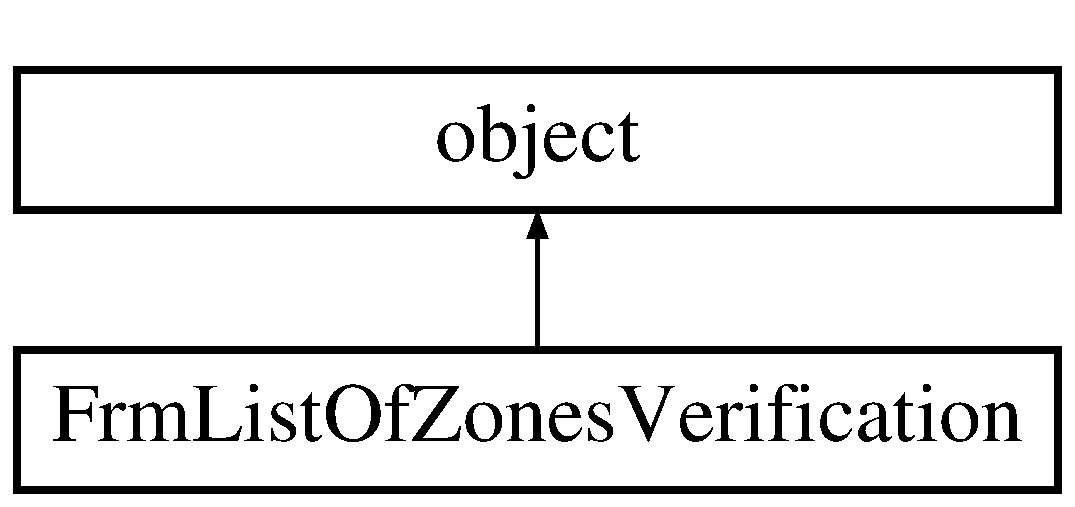
\includegraphics[height=2.000000cm]{class_f_list_of_zones_verification_1_1_frm_list_of_zones_verification}
\end{center}
\end{figure}
\subsection*{Public Member Functions}
\begin{DoxyCompactItemize}
\item 
\mbox{\Hypertarget{class_f_list_of_zones_verification_1_1_frm_list_of_zones_verification_adb8818239148d2e5c5833a2b062ee9ad}\label{class_f_list_of_zones_verification_1_1_frm_list_of_zones_verification_adb8818239148d2e5c5833a2b062ee9ad}} 
def {\bfseries ID} (self)
\item 
\mbox{\Hypertarget{class_f_list_of_zones_verification_1_1_frm_list_of_zones_verification_a10ce1b784ddb6d26ec909705cedfaaac}\label{class_f_list_of_zones_verification_1_1_frm_list_of_zones_verification_a10ce1b784ddb6d26ec909705cedfaaac}} 
def {\bfseries error} (self)
\item 
\mbox{\Hypertarget{class_f_list_of_zones_verification_1_1_frm_list_of_zones_verification_affdb4ca4609f13812474c8f022c486e3}\label{class_f_list_of_zones_verification_1_1_frm_list_of_zones_verification_affdb4ca4609f13812474c8f022c486e3}} 
def {\bfseries confirm} (self)
\item 
\mbox{\Hypertarget{class_f_list_of_zones_verification_1_1_frm_list_of_zones_verification_af418c502269da2fa1127237934c61a47}\label{class_f_list_of_zones_verification_1_1_frm_list_of_zones_verification_af418c502269da2fa1127237934c61a47}} 
def {\bfseries message} (self)
\item 
\mbox{\Hypertarget{class_f_list_of_zones_verification_1_1_frm_list_of_zones_verification_adb11456cff1807e9b8bf5d6c8d614cf6}\label{class_f_list_of_zones_verification_1_1_frm_list_of_zones_verification_adb11456cff1807e9b8bf5d6c8d614cf6}} 
def {\bfseries On\+Cancel} (self, event=None)
\item 
\mbox{\Hypertarget{class_f_list_of_zones_verification_1_1_frm_list_of_zones_verification_a1b2f2612a7fe101ab2ce06057d15d75d}\label{class_f_list_of_zones_verification_1_1_frm_list_of_zones_verification_a1b2f2612a7fe101ab2ce06057d15d75d}} 
def {\bfseries btn\+O\+K\+\_\+\+On\+Click} (self)
\item 
\mbox{\Hypertarget{class_f_list_of_zones_verification_1_1_frm_list_of_zones_verification_a09dd180e44dd70e2cef2be99bf2bf625}\label{class_f_list_of_zones_verification_1_1_frm_list_of_zones_verification_a09dd180e44dd70e2cef2be99bf2bf625}} 
def {\bfseries compare\+Lists} (self)
\item 
\mbox{\Hypertarget{class_f_list_of_zones_verification_1_1_frm_list_of_zones_verification_a3b45acb840a05589dc62ae3e2c947e94}\label{class_f_list_of_zones_verification_1_1_frm_list_of_zones_verification_a3b45acb840a05589dc62ae3e2c947e94}} 
def {\bfseries \+\_\+\+\_\+init\+\_\+\+\_\+} (self, \hyperlink{class_f_list_of_zones_verification_1_1_frm_list_of_zones_verification_a8aab264665f2085687d9eeca4c67a691}{top}, p\+Zones\+I\+DF, p\+Zones\+G\+UI)
\end{DoxyCompactItemize}
\subsection*{Public Attributes}
\begin{DoxyCompactItemize}
\item 
\mbox{\Hypertarget{class_f_list_of_zones_verification_1_1_frm_list_of_zones_verification_a8aab264665f2085687d9eeca4c67a691}\label{class_f_list_of_zones_verification_1_1_frm_list_of_zones_verification_a8aab264665f2085687d9eeca4c67a691}} 
\hyperlink{class_f_list_of_zones_verification_1_1_frm_list_of_zones_verification_a8aab264665f2085687d9eeca4c67a691}{top}
\begin{DoxyCompactList}\small\item\em colours, icons \end{DoxyCompactList}\item 
\mbox{\Hypertarget{class_f_list_of_zones_verification_1_1_frm_list_of_zones_verification_a026309584087467d71c3f4af14102b44}\label{class_f_list_of_zones_verification_1_1_frm_list_of_zones_verification_a026309584087467d71c3f4af14102b44}} 
{\bfseries btn\+Cancel}
\item 
\mbox{\Hypertarget{class_f_list_of_zones_verification_1_1_frm_list_of_zones_verification_ad51735611b2c34fc0d40826fca86792f}\label{class_f_list_of_zones_verification_1_1_frm_list_of_zones_verification_ad51735611b2c34fc0d40826fca86792f}} 
{\bfseries btn\+OK}
\item 
\mbox{\Hypertarget{class_f_list_of_zones_verification_1_1_frm_list_of_zones_verification_a7194e145aa133aecee0d04b652d24af5}\label{class_f_list_of_zones_verification_1_1_frm_list_of_zones_verification_a7194e145aa133aecee0d04b652d24af5}} 
{\bfseries lblzones\+I\+DF}
\item 
\mbox{\Hypertarget{class_f_list_of_zones_verification_1_1_frm_list_of_zones_verification_a53b27ef4d747d97fcf907ff9655e196b}\label{class_f_list_of_zones_verification_1_1_frm_list_of_zones_verification_a53b27ef4d747d97fcf907ff9655e196b}} 
{\bfseries lst\+Zones\+I\+DF}
\item 
\mbox{\Hypertarget{class_f_list_of_zones_verification_1_1_frm_list_of_zones_verification_ab1fcf7a15678faa03a804f63bb2e38e8}\label{class_f_list_of_zones_verification_1_1_frm_list_of_zones_verification_ab1fcf7a15678faa03a804f63bb2e38e8}} 
{\bfseries lblzones\+G\+UI}
\item 
\mbox{\Hypertarget{class_f_list_of_zones_verification_1_1_frm_list_of_zones_verification_a36c97b561df0d74433f8f8a262be3d88}\label{class_f_list_of_zones_verification_1_1_frm_list_of_zones_verification_a36c97b561df0d74433f8f8a262be3d88}} 
{\bfseries lst\+Zones\+G\+UI}
\item 
\mbox{\Hypertarget{class_f_list_of_zones_verification_1_1_frm_list_of_zones_verification_a356732ea4633bf7934c35bc6ad78170c}\label{class_f_list_of_zones_verification_1_1_frm_list_of_zones_verification_a356732ea4633bf7934c35bc6ad78170c}} 
{\bfseries lbl\+Message}
\end{DoxyCompactItemize}


\subsection{Detailed Description}


Definition at line 20 of file F\+List\+Of\+Zones\+Verification.\+py.



The documentation for this class was generated from the following file\+:\begin{DoxyCompactItemize}
\item 
F\+List\+Of\+Zones\+Verification.\+py\end{DoxyCompactItemize}

\hypertarget{class_f_log_1_1_frm_log}{}\section{Frm\+Log Class Reference}
\label{class_f_log_1_1_frm_log}\index{Frm\+Log@{Frm\+Log}}
Inheritance diagram for Frm\+Log\+:\begin{figure}[H]
\begin{center}
\leavevmode
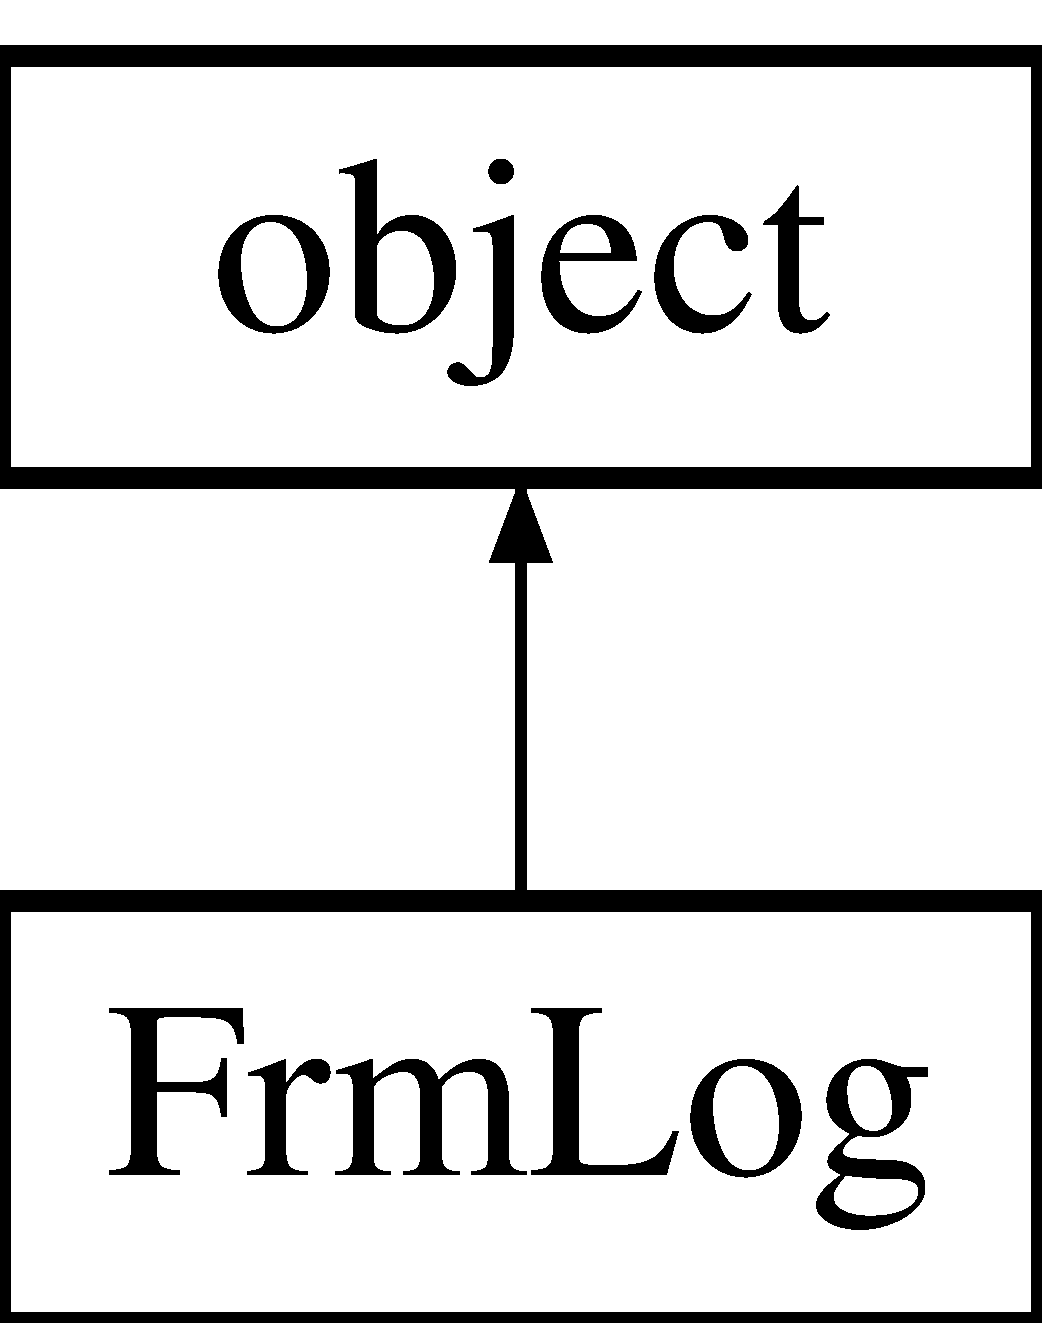
\includegraphics[height=2.000000cm]{class_f_log_1_1_frm_log}
\end{center}
\end{figure}
\subsection*{Public Member Functions}
\begin{DoxyCompactItemize}
\item 
\mbox{\Hypertarget{class_f_log_1_1_frm_log_adb8818239148d2e5c5833a2b062ee9ad}\label{class_f_log_1_1_frm_log_adb8818239148d2e5c5833a2b062ee9ad}} 
def {\bfseries ID} (self)
\item 
\mbox{\Hypertarget{class_f_log_1_1_frm_log_a9e7a6618d4b693eb2dab68e2f34a7886}\label{class_f_log_1_1_frm_log_a9e7a6618d4b693eb2dab68e2f34a7886}} 
def {\bfseries write} (self, value)
\item 
\mbox{\Hypertarget{class_f_log_1_1_frm_log_a75020e7f3888d6f837fae592b305add8}\label{class_f_log_1_1_frm_log_a75020e7f3888d6f837fae592b305add8}} 
def {\bfseries \+\_\+\+\_\+init\+\_\+\+\_\+} (self, parent)
\end{DoxyCompactItemize}
\subsection*{Public Attributes}
\begin{DoxyCompactItemize}
\item 
\mbox{\Hypertarget{class_f_log_1_1_frm_log_a06feb554f3bbbe630438139278982556}\label{class_f_log_1_1_frm_log_a06feb554f3bbbe630438139278982556}} 
{\bfseries txt\+Log}
\end{DoxyCompactItemize}


\subsection{Detailed Description}


Definition at line 12 of file F\+Log.\+py.



The documentation for this class was generated from the following file\+:\begin{DoxyCompactItemize}
\item 
F\+Log.\+py\end{DoxyCompactItemize}

\hypertarget{class_f_occupant_1_1_frm_occupant}{}\section{Frm\+Occupant Class Reference}
\label{class_f_occupant_1_1_frm_occupant}\index{Frm\+Occupant@{Frm\+Occupant}}
Inheritance diagram for Frm\+Occupant\+:\begin{figure}[H]
\begin{center}
\leavevmode
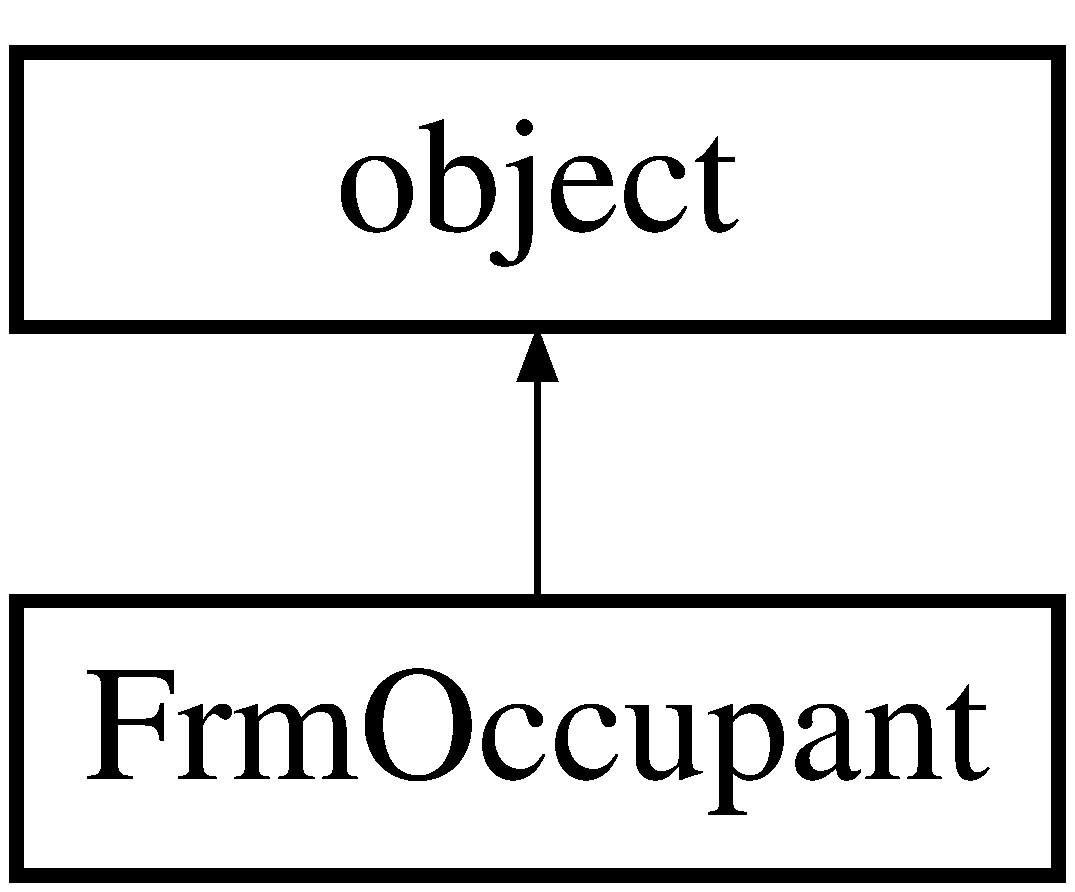
\includegraphics[height=2.000000cm]{class_f_occupant_1_1_frm_occupant}
\end{center}
\end{figure}
\subsection*{Public Member Functions}
\begin{DoxyCompactItemize}
\item 
\mbox{\Hypertarget{class_f_occupant_1_1_frm_occupant_a77f9e90492436b634a669b1c9736c385}\label{class_f_occupant_1_1_frm_occupant_a77f9e90492436b634a669b1c9736c385}} 
def {\bfseries load} (self, id=None, name=None, description=None, category\+ID=None, category=None, region\+ID=None, region=None, sector\+ID=None, sector=None, occupants=None, zones=None, show=False, enabled=False)
\item 
\mbox{\Hypertarget{class_f_occupant_1_1_frm_occupant_afce1a505a79b9242ea0063c7be848e01}\label{class_f_occupant_1_1_frm_occupant_afce1a505a79b9242ea0063c7be848e01}} 
def {\bfseries update\+Zone\+List} (self, zones)
\item 
\mbox{\Hypertarget{class_f_occupant_1_1_frm_occupant_ab4f4398c3f210fe4ea6e720401357691}\label{class_f_occupant_1_1_frm_occupant_ab4f4398c3f210fe4ea6e720401357691}} 
def {\bfseries show} (self)
\item 
\mbox{\Hypertarget{class_f_occupant_1_1_frm_occupant_af9ea366b42c0f2b7b33d109814e3cfa1}\label{class_f_occupant_1_1_frm_occupant_af9ea366b42c0f2b7b33d109814e3cfa1}} 
def {\bfseries \+\_\+\+\_\+init\+\_\+\+\_\+} (self, master, parent, uuid=str(uuid.\+uuid4()), id=0, name=\textquotesingle{}\textquotesingle{}, description=\textquotesingle{}\textquotesingle{}, category\+ID=\textquotesingle{}\textquotesingle{}, category=\textquotesingle{}\textquotesingle{}, region\+ID=\textquotesingle{}\textquotesingle{}, region=\textquotesingle{}\textquotesingle{}, sector\+ID=\textquotesingle{}\textquotesingle{}, sector=\textquotesingle{}\textquotesingle{}, power=0, zone\+Id=\textquotesingle{}\textquotesingle{}, occupants=None, zones=\{\char`\"{}undefined\char`\"{}\+:\char`\"{}undefinded\char`\"{}\})
\end{DoxyCompactItemize}
\subsection*{Public Attributes}
\begin{DoxyCompactItemize}
\item 
\mbox{\Hypertarget{class_f_occupant_1_1_frm_occupant_ab7f21eb3200b90c22d0814ef7446db99}\label{class_f_occupant_1_1_frm_occupant_ab7f21eb3200b90c22d0814ef7446db99}} 
{\bfseries tab\+General}
\item 
\mbox{\Hypertarget{class_f_occupant_1_1_frm_occupant_adf48681793bddd9a9471ece209412d9b}\label{class_f_occupant_1_1_frm_occupant_adf48681793bddd9a9471ece209412d9b}} 
{\bfseries tab\+Occupant}
\item 
\mbox{\Hypertarget{class_f_occupant_1_1_frm_occupant_afe9b98e5038ae1c69e5bb7eef0ed7cc4}\label{class_f_occupant_1_1_frm_occupant_afe9b98e5038ae1c69e5bb7eef0ed7cc4}} 
{\bfseries lblname}
\item 
\mbox{\Hypertarget{class_f_occupant_1_1_frm_occupant_a24025fc9f698a9db8fb4f3c1c3c32e40}\label{class_f_occupant_1_1_frm_occupant_a24025fc9f698a9db8fb4f3c1c3c32e40}} 
{\bfseries txtname}
\item 
\mbox{\Hypertarget{class_f_occupant_1_1_frm_occupant_ab1b41c78341955dad7992f80dede5cb1}\label{class_f_occupant_1_1_frm_occupant_ab1b41c78341955dad7992f80dede5cb1}} 
{\bfseries lbldescription}
\item 
\mbox{\Hypertarget{class_f_occupant_1_1_frm_occupant_ae2475afd1e25ae07fbd937e3456d25d7}\label{class_f_occupant_1_1_frm_occupant_ae2475afd1e25ae07fbd937e3456d25d7}} 
{\bfseries txtdescription}
\item 
\mbox{\Hypertarget{class_f_occupant_1_1_frm_occupant_a161a89218ee83fb033733ecac11a4d00}\label{class_f_occupant_1_1_frm_occupant_a161a89218ee83fb033733ecac11a4d00}} 
{\bfseries lblsector}
\item 
\mbox{\Hypertarget{class_f_occupant_1_1_frm_occupant_a932eda1eaef9afc4a195d6e88ccc4e83}\label{class_f_occupant_1_1_frm_occupant_a932eda1eaef9afc4a195d6e88ccc4e83}} 
{\bfseries ddl\+Sector}
\item 
\mbox{\Hypertarget{class_f_occupant_1_1_frm_occupant_ad385f1a04fffd7bfa2bf34a29ffc6d24}\label{class_f_occupant_1_1_frm_occupant_ad385f1a04fffd7bfa2bf34a29ffc6d24}} 
{\bfseries lblregion}
\item 
\mbox{\Hypertarget{class_f_occupant_1_1_frm_occupant_a2908c047368850827dd367d2b7834f44}\label{class_f_occupant_1_1_frm_occupant_a2908c047368850827dd367d2b7834f44}} 
{\bfseries ddl\+Region}
\item 
\mbox{\Hypertarget{class_f_occupant_1_1_frm_occupant_aa67f411cdded7720745bddc6554ccfa1}\label{class_f_occupant_1_1_frm_occupant_aa67f411cdded7720745bddc6554ccfa1}} 
{\bfseries lblcategory}
\item 
\mbox{\Hypertarget{class_f_occupant_1_1_frm_occupant_a773267719f8b87725ebc5461cbab0bdc}\label{class_f_occupant_1_1_frm_occupant_a773267719f8b87725ebc5461cbab0bdc}} 
{\bfseries ddl\+Category}
\item 
\mbox{\Hypertarget{class_f_occupant_1_1_frm_occupant_a944801cc442d2670e4905a3dbee97ad0}\label{class_f_occupant_1_1_frm_occupant_a944801cc442d2670e4905a3dbee97ad0}} 
{\bfseries lblzone}
\item 
\mbox{\Hypertarget{class_f_occupant_1_1_frm_occupant_a6866aa92e7eadd533576089d401e8dc4}\label{class_f_occupant_1_1_frm_occupant_a6866aa92e7eadd533576089d401e8dc4}} 
{\bfseries ddl\+Zone}
\item 
\mbox{\Hypertarget{class_f_occupant_1_1_frm_occupant_a2de24e637e40e02c22532f626730698a}\label{class_f_occupant_1_1_frm_occupant_a2de24e637e40e02c22532f626730698a}} 
{\bfseries lblpower}
\item 
\mbox{\Hypertarget{class_f_occupant_1_1_frm_occupant_ab6a1c082bfaadf3c7efe7e5de17b9a9e}\label{class_f_occupant_1_1_frm_occupant_ab6a1c082bfaadf3c7efe7e5de17b9a9e}} 
{\bfseries txt\+Power}
\item 
\mbox{\Hypertarget{class_f_occupant_1_1_frm_occupant_a8636f68b352f4c867d8509cf1f07faf3}\label{class_f_occupant_1_1_frm_occupant_a8636f68b352f4c867d8509cf1f07faf3}} 
{\bfseries lblwindow\+Id}
\item 
\mbox{\Hypertarget{class_f_occupant_1_1_frm_occupant_a712d3641bf7b2b22043e27e90ce8f7db}\label{class_f_occupant_1_1_frm_occupant_a712d3641bf7b2b22043e27e90ce8f7db}} 
{\bfseries ddl\+Window}
\item 
\mbox{\Hypertarget{class_f_occupant_1_1_frm_occupant_a56ff5b38995d7f89d2fa714da6a4ce6d}\label{class_f_occupant_1_1_frm_occupant_a56ff5b38995d7f89d2fa714da6a4ce6d}} 
{\bfseries lblshade\+Id}
\item 
\mbox{\Hypertarget{class_f_occupant_1_1_frm_occupant_aca11b590bf7e97dc2c390ec61ec022cd}\label{class_f_occupant_1_1_frm_occupant_aca11b590bf7e97dc2c390ec61ec022cd}} 
{\bfseries ddl\+Shade}
\item 
\mbox{\Hypertarget{class_f_occupant_1_1_frm_occupant_a8cf4ad97e9fe70954d930560fd96db8f}\label{class_f_occupant_1_1_frm_occupant_a8cf4ad97e9fe70954d930560fd96db8f}} 
{\bfseries lblsex}
\item 
\mbox{\Hypertarget{class_f_occupant_1_1_frm_occupant_a2828ba9b6fb1c4d5bee707b3a7a9b305}\label{class_f_occupant_1_1_frm_occupant_a2828ba9b6fb1c4d5bee707b3a7a9b305}} 
{\bfseries ddl\+Gender}
\item 
\mbox{\Hypertarget{class_f_occupant_1_1_frm_occupant_a2b21ef75baa9e525b9552008180a26ec}\label{class_f_occupant_1_1_frm_occupant_a2b21ef75baa9e525b9552008180a26ec}} 
{\bfseries lblfamily\+ID}
\item 
\mbox{\Hypertarget{class_f_occupant_1_1_frm_occupant_a7d619a44dfacda4882d4fc0dae3a1dfc}\label{class_f_occupant_1_1_frm_occupant_a7d619a44dfacda4882d4fc0dae3a1dfc}} 
{\bfseries ddl\+Family}
\item 
\mbox{\Hypertarget{class_f_occupant_1_1_frm_occupant_ac49f679b7ef0139c3eb136e5189a4af5}\label{class_f_occupant_1_1_frm_occupant_ac49f679b7ef0139c3eb136e5189a4af5}} 
{\bfseries lbleducation\+ID}
\item 
\mbox{\Hypertarget{class_f_occupant_1_1_frm_occupant_a90765f81d94854f567fc1897dc56e860}\label{class_f_occupant_1_1_frm_occupant_a90765f81d94854f567fc1897dc56e860}} 
{\bfseries ddl\+Education}
\item 
\mbox{\Hypertarget{class_f_occupant_1_1_frm_occupant_aebedf27420635e9639cfce9b9d41f908}\label{class_f_occupant_1_1_frm_occupant_aebedf27420635e9639cfce9b9d41f908}} 
{\bfseries lblage\+ID}
\item 
\mbox{\Hypertarget{class_f_occupant_1_1_frm_occupant_aa0788a911a181183974abfd7aff8b3f3}\label{class_f_occupant_1_1_frm_occupant_aa0788a911a181183974abfd7aff8b3f3}} 
{\bfseries ddl\+Age}
\item 
\mbox{\Hypertarget{class_f_occupant_1_1_frm_occupant_a67abcc6287cbbefb1143571682eb2158}\label{class_f_occupant_1_1_frm_occupant_a67abcc6287cbbefb1143571682eb2158}} 
{\bfseries lblown\+Computer}
\item 
\mbox{\Hypertarget{class_f_occupant_1_1_frm_occupant_a8e9d9ee98eae06c7ca0654b5b4d3f5bc}\label{class_f_occupant_1_1_frm_occupant_a8e9d9ee98eae06c7ca0654b5b4d3f5bc}} 
{\bfseries chk\+Own\+Computer}
\item 
\mbox{\Hypertarget{class_f_occupant_1_1_frm_occupant_ad2cd2cb636e6ff74ca5d1ebc74fb6aba}\label{class_f_occupant_1_1_frm_occupant_ad2cd2cb636e6ff74ca5d1ebc74fb6aba}} 
{\bfseries lblis\+Retired}
\item 
\mbox{\Hypertarget{class_f_occupant_1_1_frm_occupant_aa0f9ea0cacfbbfd3ad742f9e058a328d}\label{class_f_occupant_1_1_frm_occupant_aa0f9ea0cacfbbfd3ad742f9e058a328d}} 
{\bfseries chk\+Is\+Retired}
\item 
\mbox{\Hypertarget{class_f_occupant_1_1_frm_occupant_a34af38285450b3293b4f7de025ccc98b}\label{class_f_occupant_1_1_frm_occupant_a34af38285450b3293b4f7de025ccc98b}} 
{\bfseries lblis\+Married}
\item 
\mbox{\Hypertarget{class_f_occupant_1_1_frm_occupant_af64bb6ab006e18701d6608114eb4fc87}\label{class_f_occupant_1_1_frm_occupant_af64bb6ab006e18701d6608114eb4fc87}} 
{\bfseries chk\+Is\+Married}
\item 
\mbox{\Hypertarget{class_f_occupant_1_1_frm_occupant_a9643b8c0a42bd97c33043dc367a776af}\label{class_f_occupant_1_1_frm_occupant_a9643b8c0a42bd97c33043dc367a776af}} 
{\bfseries lblis\+Un\+Employed}
\item 
\mbox{\Hypertarget{class_f_occupant_1_1_frm_occupant_aff560f3f01994103c88d7e44bda65316}\label{class_f_occupant_1_1_frm_occupant_aff560f3f01994103c88d7e44bda65316}} 
{\bfseries chk\+Is\+Employed}
\end{DoxyCompactItemize}


\subsection{Detailed Description}


Definition at line 14 of file F\+Occupant.\+py.



The documentation for this class was generated from the following file\+:\begin{DoxyCompactItemize}
\item 
F\+Occupant.\+py\end{DoxyCompactItemize}

\hypertarget{class_f_occupant_templates_1_1_frm_occupant_templates}{}\section{Frm\+Occupant\+Templates Class Reference}
\label{class_f_occupant_templates_1_1_frm_occupant_templates}\index{Frm\+Occupant\+Templates@{Frm\+Occupant\+Templates}}
Inheritance diagram for Frm\+Occupant\+Templates\+:\begin{figure}[H]
\begin{center}
\leavevmode
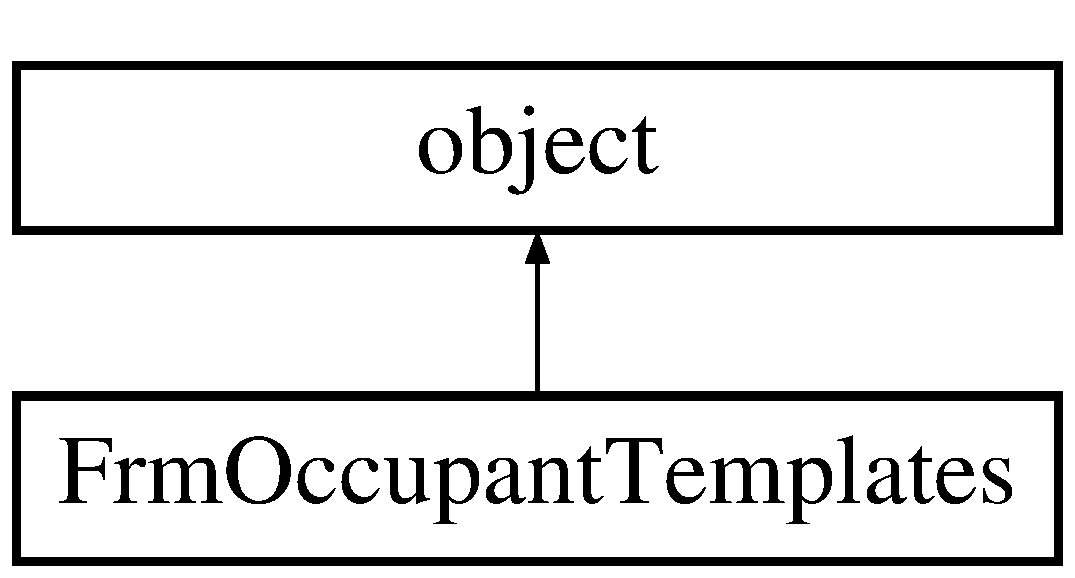
\includegraphics[height=2.000000cm]{class_f_occupant_templates_1_1_frm_occupant_templates}
\end{center}
\end{figure}
\subsection*{Public Member Functions}
\begin{DoxyCompactItemize}
\item 
\mbox{\Hypertarget{class_f_occupant_templates_1_1_frm_occupant_templates_adb8818239148d2e5c5833a2b062ee9ad}\label{class_f_occupant_templates_1_1_frm_occupant_templates_adb8818239148d2e5c5833a2b062ee9ad}} 
def {\bfseries ID} (self)
\item 
\mbox{\Hypertarget{class_f_occupant_templates_1_1_frm_occupant_templates_a10ce1b784ddb6d26ec909705cedfaaac}\label{class_f_occupant_templates_1_1_frm_occupant_templates_a10ce1b784ddb6d26ec909705cedfaaac}} 
def {\bfseries error} (self)
\item 
\mbox{\Hypertarget{class_f_occupant_templates_1_1_frm_occupant_templates_af418c502269da2fa1127237934c61a47}\label{class_f_occupant_templates_1_1_frm_occupant_templates_af418c502269da2fa1127237934c61a47}} 
def {\bfseries message} (self)
\item 
\mbox{\Hypertarget{class_f_occupant_templates_1_1_frm_occupant_templates_a2731ba3d3e529a962bfdccaf2cfd3b0e}\label{class_f_occupant_templates_1_1_frm_occupant_templates_a2731ba3d3e529a962bfdccaf2cfd3b0e}} 
def {\bfseries template} (self)
\item 
\mbox{\Hypertarget{class_f_occupant_templates_1_1_frm_occupant_templates_a8be5fb323a7bfaa1f705bf57d44452d4}\label{class_f_occupant_templates_1_1_frm_occupant_templates_a8be5fb323a7bfaa1f705bf57d44452d4}} 
def {\bfseries clear\+Occupants\+Tab} (self)
\item 
\mbox{\Hypertarget{class_f_occupant_templates_1_1_frm_occupant_templates_a526766a161d0422f905eb841dd256560}\label{class_f_occupant_templates_1_1_frm_occupant_templates_a526766a161d0422f905eb841dd256560}} 
def {\bfseries load\+Empty\+Template} (self)
\item 
\mbox{\Hypertarget{class_f_occupant_templates_1_1_frm_occupant_templates_a0685140bf253e931091601a4f5ec7b53}\label{class_f_occupant_templates_1_1_frm_occupant_templates_a0685140bf253e931091601a4f5ec7b53}} 
def {\bfseries tvw\+Templates\+\_\+\+On\+Node\+Expand} (self, event)
\item 
\mbox{\Hypertarget{class_f_occupant_templates_1_1_frm_occupant_templates_ac7d8328625c6f9850aafbe63e6d20a37}\label{class_f_occupant_templates_1_1_frm_occupant_templates_ac7d8328625c6f9850aafbe63e6d20a37}} 
def {\bfseries tvw\+Templates\+\_\+\+On\+Node\+Collapse} (self, event)
\item 
\mbox{\Hypertarget{class_f_occupant_templates_1_1_frm_occupant_templates_a4bb373616966dd5afafb70800b5940ed}\label{class_f_occupant_templates_1_1_frm_occupant_templates_a4bb373616966dd5afafb70800b5940ed}} 
def {\bfseries tvw\+Templates\+\_\+\+On\+Node\+Select} (self, event)
\item 
\mbox{\Hypertarget{class_f_occupant_templates_1_1_frm_occupant_templates_adb11456cff1807e9b8bf5d6c8d614cf6}\label{class_f_occupant_templates_1_1_frm_occupant_templates_adb11456cff1807e9b8bf5d6c8d614cf6}} 
def {\bfseries On\+Cancel} (self, event=None)
\item 
\mbox{\Hypertarget{class_f_occupant_templates_1_1_frm_occupant_templates_a8b8ae7c9b7218399271e449584fc28f9}\label{class_f_occupant_templates_1_1_frm_occupant_templates_a8b8ae7c9b7218399271e449584fc28f9}} 
def {\bfseries load\+Templates\+From\+File} (self)
\item 
\mbox{\Hypertarget{class_f_occupant_templates_1_1_frm_occupant_templates_a3f7101570014b9e7858ba3fb83c8286a}\label{class_f_occupant_templates_1_1_frm_occupant_templates_a3f7101570014b9e7858ba3fb83c8286a}} 
def {\bfseries get\+Template} (self, template\+ID)
\item 
\mbox{\Hypertarget{class_f_occupant_templates_1_1_frm_occupant_templates_ad954cbff8c08e311d8bbe4efc4440ba6}\label{class_f_occupant_templates_1_1_frm_occupant_templates_ad954cbff8c08e311d8bbe4efc4440ba6}} 
def {\bfseries txt\+Power\+\_\+\+On\+Power\+Changed} (self, sender)
\item 
\mbox{\Hypertarget{class_f_occupant_templates_1_1_frm_occupant_templates_a1b2f2612a7fe101ab2ce06057d15d75d}\label{class_f_occupant_templates_1_1_frm_occupant_templates_a1b2f2612a7fe101ab2ce06057d15d75d}} 
def {\bfseries btn\+O\+K\+\_\+\+On\+Click} (self)
\item 
\mbox{\Hypertarget{class_f_occupant_templates_1_1_frm_occupant_templates_a90fe6dc8a438aa5b415daef88808e5f4}\label{class_f_occupant_templates_1_1_frm_occupant_templates_a90fe6dc8a438aa5b415daef88808e5f4}} 
def {\bfseries \+\_\+\+\_\+init\+\_\+\+\_\+} (self, \hyperlink{class_f_occupant_templates_1_1_frm_occupant_templates_a8aab264665f2085687d9eeca4c67a691}{top}, p\+Zones, value=None)
\end{DoxyCompactItemize}
\subsection*{Public Attributes}
\begin{DoxyCompactItemize}
\item 
\hyperlink{class_f_occupant_templates_1_1_frm_occupant_templates_a8aab264665f2085687d9eeca4c67a691}{top}
\begin{DoxyCompactList}\small\item\em configuration self.\+style = ttk.\+Style() if sys.\+platform == \char`\"{}win32\char`\"{}\+: self.\+style.\+theme\+\_\+use(\textquotesingle{}winnative\textquotesingle{}) self.\+style.\+configure(\textquotesingle{}. \end{DoxyCompactList}\item 
\mbox{\Hypertarget{class_f_occupant_templates_1_1_frm_occupant_templates_a707f220a2b61183c6209feef648f12da}\label{class_f_occupant_templates_1_1_frm_occupant_templates_a707f220a2b61183c6209feef648f12da}} 
{\bfseries tvw\+Templates}
\item 
\mbox{\Hypertarget{class_f_occupant_templates_1_1_frm_occupant_templates_a026309584087467d71c3f4af14102b44}\label{class_f_occupant_templates_1_1_frm_occupant_templates_a026309584087467d71c3f4af14102b44}} 
{\bfseries btn\+Cancel}
\item 
\mbox{\Hypertarget{class_f_occupant_templates_1_1_frm_occupant_templates_ad51735611b2c34fc0d40826fca86792f}\label{class_f_occupant_templates_1_1_frm_occupant_templates_ad51735611b2c34fc0d40826fca86792f}} 
{\bfseries btn\+OK}
\item 
\mbox{\Hypertarget{class_f_occupant_templates_1_1_frm_occupant_templates_a8a52430ec740c576d2ff73adcc56887b}\label{class_f_occupant_templates_1_1_frm_occupant_templates_a8a52430ec740c576d2ff73adcc56887b}} 
{\bfseries data\+Container}
\item 
\mbox{\Hypertarget{class_f_occupant_templates_1_1_frm_occupant_templates_ab7f21eb3200b90c22d0814ef7446db99}\label{class_f_occupant_templates_1_1_frm_occupant_templates_ab7f21eb3200b90c22d0814ef7446db99}} 
{\bfseries tab\+General}
\item 
\mbox{\Hypertarget{class_f_occupant_templates_1_1_frm_occupant_templates_a29330eb364e759b8e3a98d0929258003}\label{class_f_occupant_templates_1_1_frm_occupant_templates_a29330eb364e759b8e3a98d0929258003}} 
{\bfseries tab\+Occupants}
\item 
\mbox{\Hypertarget{class_f_occupant_templates_1_1_frm_occupant_templates_a570b8f6946403d60d00cfcafd914d6bd}\label{class_f_occupant_templates_1_1_frm_occupant_templates_a570b8f6946403d60d00cfcafd914d6bd}} 
{\bfseries txt\+Name}
\item 
\mbox{\Hypertarget{class_f_occupant_templates_1_1_frm_occupant_templates_a077ff90d6e1ad5952cf3fdf11425850c}\label{class_f_occupant_templates_1_1_frm_occupant_templates_a077ff90d6e1ad5952cf3fdf11425850c}} 
{\bfseries txt\+Description}
\item 
\mbox{\Hypertarget{class_f_occupant_templates_1_1_frm_occupant_templates_a932eda1eaef9afc4a195d6e88ccc4e83}\label{class_f_occupant_templates_1_1_frm_occupant_templates_a932eda1eaef9afc4a195d6e88ccc4e83}} 
{\bfseries ddl\+Sector}
\item 
\mbox{\Hypertarget{class_f_occupant_templates_1_1_frm_occupant_templates_a2908c047368850827dd367d2b7834f44}\label{class_f_occupant_templates_1_1_frm_occupant_templates_a2908c047368850827dd367d2b7834f44}} 
{\bfseries ddl\+Region}
\item 
\mbox{\Hypertarget{class_f_occupant_templates_1_1_frm_occupant_templates_a773267719f8b87725ebc5461cbab0bdc}\label{class_f_occupant_templates_1_1_frm_occupant_templates_a773267719f8b87725ebc5461cbab0bdc}} 
{\bfseries ddl\+Category}
\end{DoxyCompactItemize}


\subsection{Detailed Description}


Definition at line 17 of file F\+Occupant\+Templates.\+py.



\subsection{Member Data Documentation}
\mbox{\Hypertarget{class_f_occupant_templates_1_1_frm_occupant_templates_a8aab264665f2085687d9eeca4c67a691}\label{class_f_occupant_templates_1_1_frm_occupant_templates_a8aab264665f2085687d9eeca4c67a691}} 
\index{F\+Occupant\+Templates\+::\+Frm\+Occupant\+Templates@{F\+Occupant\+Templates\+::\+Frm\+Occupant\+Templates}!top@{top}}
\index{top@{top}!F\+Occupant\+Templates\+::\+Frm\+Occupant\+Templates@{F\+Occupant\+Templates\+::\+Frm\+Occupant\+Templates}}
\subsubsection{\texorpdfstring{top}{top}}
{\footnotesize\ttfamily top}



configuration self.\+style = ttk.\+Style() if sys.\+platform == \char`\"{}win32\char`\"{}\+: self.\+style.\+theme\+\_\+use(\textquotesingle{}winnative\textquotesingle{}) self.\+style.\+configure(\textquotesingle{}. 

\textquotesingle{},background=\+\_\+bgcolor) self.\+style.\+configure(\textquotesingle{}.\textquotesingle{},foreground=\+\_\+fgcolor) self.\+style.\+configure(\textquotesingle{}.\textquotesingle{},font=\char`\"{}\+Tk\+Default\+Font\char`\"{}) self.\+style.\+map(\textquotesingle{}.\textquotesingle{},background= \mbox{[}(\textquotesingle{}selected\textquotesingle{}, \+\_\+compcolor), (\textquotesingle{}active\textquotesingle{},\+\_\+ana2color)\mbox{]}) 

Definition at line 377 of file F\+Occupant\+Templates.\+py.



The documentation for this class was generated from the following file\+:\begin{DoxyCompactItemize}
\item 
F\+Occupant\+Templates.\+py\end{DoxyCompactItemize}

\hypertarget{class_f_plots_1_1_frm_plots}{}\section{Frm\+Plots Class Reference}
\label{class_f_plots_1_1_frm_plots}\index{Frm\+Plots@{Frm\+Plots}}
Inheritance diagram for Frm\+Plots\+:\begin{figure}[H]
\begin{center}
\leavevmode
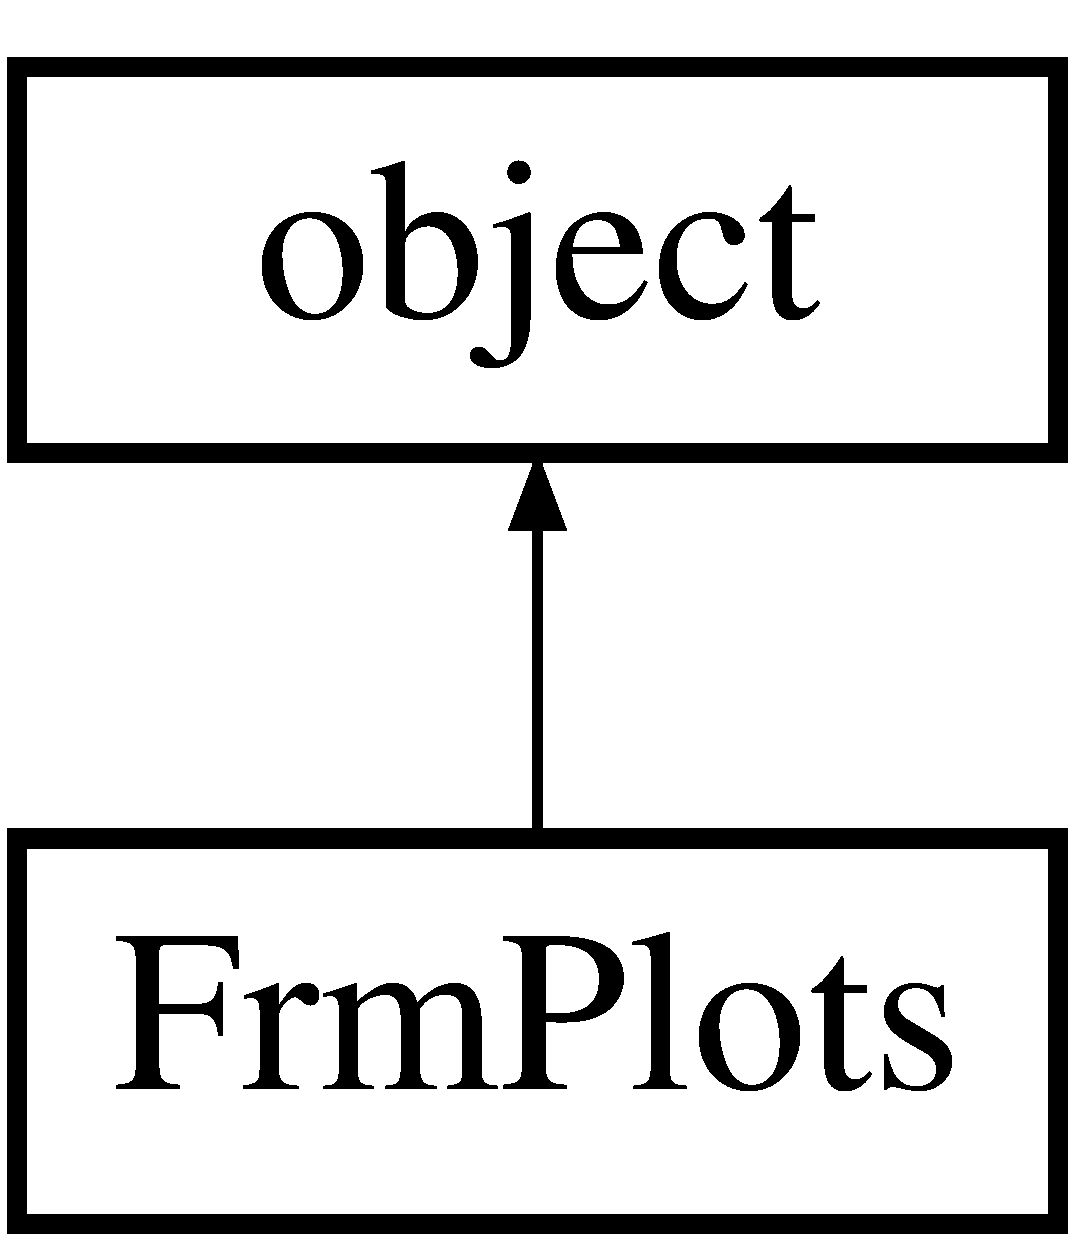
\includegraphics[height=2.000000cm]{class_f_plots_1_1_frm_plots}
\end{center}
\end{figure}
\subsection*{Public Member Functions}
\begin{DoxyCompactItemize}
\item 
\mbox{\Hypertarget{class_f_plots_1_1_frm_plots_adb8818239148d2e5c5833a2b062ee9ad}\label{class_f_plots_1_1_frm_plots_adb8818239148d2e5c5833a2b062ee9ad}} 
def {\bfseries ID} (self)
\item 
\mbox{\Hypertarget{class_f_plots_1_1_frm_plots_acf44064249ee17c3e8952b4c33512f86}\label{class_f_plots_1_1_frm_plots_acf44064249ee17c3e8952b4c33512f86}} 
def {\bfseries Frame} (self)
\item 
\mbox{\Hypertarget{class_f_plots_1_1_frm_plots_a3af7bd47020a22de652781d72c19a265}\label{class_f_plots_1_1_frm_plots_a3af7bd47020a22de652781d72c19a265}} 
def {\bfseries select\+Output\+Directory} (self)
\item 
\mbox{\Hypertarget{class_f_plots_1_1_frm_plots_acf90b44776d8669c402087788d5246fb}\label{class_f_plots_1_1_frm_plots_acf90b44776d8669c402087788d5246fb}} 
def {\bfseries load\+Simulations\+And\+Plot} (self)
\item 
\mbox{\Hypertarget{class_f_plots_1_1_frm_plots_a27780f47ca6f6a3b9b6c8b2475eec865}\label{class_f_plots_1_1_frm_plots_a27780f47ca6f6a3b9b6c8b2475eec865}} 
def {\bfseries load\+Area\+Per\+Zone} (self)
\item 
\mbox{\Hypertarget{class_f_plots_1_1_frm_plots_a95c298b0291c27af5d40f1a40dca8f0b}\label{class_f_plots_1_1_frm_plots_a95c298b0291c27af5d40f1a40dca8f0b}} 
def {\bfseries load\+Simulation} (self)
\item 
\mbox{\Hypertarget{class_f_plots_1_1_frm_plots_a9bdc9f98fcbe640957caca266a3e0f0a}\label{class_f_plots_1_1_frm_plots_a9bdc9f98fcbe640957caca266a3e0f0a}} 
def {\bfseries export\+Variable} (self)
\item 
\mbox{\Hypertarget{class_f_plots_1_1_frm_plots_a834376d8212664e7208c644d0a36f1c8}\label{class_f_plots_1_1_frm_plots_a834376d8212664e7208c644d0a36f1c8}} 
def {\bfseries get\+Variable\+Name} (self, variable\+Name, period\+Type)
\item 
\mbox{\Hypertarget{class_f_plots_1_1_frm_plots_acf73ddfd8b8ce73ddeb8a362b41a55ec}\label{class_f_plots_1_1_frm_plots_acf73ddfd8b8ce73ddeb8a362b41a55ec}} 
def {\bfseries convert\+Jules\+To\+W\+MS} (self, value, area)
\item 
\mbox{\Hypertarget{class_f_plots_1_1_frm_plots_af7683488b51773e23270b5cdd3380c8c}\label{class_f_plots_1_1_frm_plots_af7683488b51773e23270b5cdd3380c8c}} 
def {\bfseries do\+Plot} (self, root\+Folder, parent\+Folder, no\+Replicates, period\+Type, var\+Name, b\+Plot\+All\+Zones, ts\+P\+Hour)
\item 
\mbox{\Hypertarget{class_f_plots_1_1_frm_plots_a9dcb77423e5f2f8ca4e2941947a418c9}\label{class_f_plots_1_1_frm_plots_a9dcb77423e5f2f8ca4e2941947a418c9}} 
def {\bfseries tvw\+Output\+Variables\+\_\+\+On\+Double\+Click\+Item} (self, event=None)
\item 
\mbox{\Hypertarget{class_f_plots_1_1_frm_plots_a9122a2b5fbc4bca093af108dab691906}\label{class_f_plots_1_1_frm_plots_a9122a2b5fbc4bca093af108dab691906}} 
def {\bfseries \+\_\+\+\_\+init\+\_\+\+\_\+} (self, master, parent, obj\+Simulation)
\end{DoxyCompactItemize}
\subsection*{Public Attributes}
\begin{DoxyCompactItemize}
\item 
\mbox{\Hypertarget{class_f_plots_1_1_frm_plots_a7bf7bb97f47ddff4363c79517bb55363}\label{class_f_plots_1_1_frm_plots_a7bf7bb97f47ddff4363c79517bb55363}} 
{\bfseries period}
\item 
\mbox{\Hypertarget{class_f_plots_1_1_frm_plots_a461765f411eafd042ce73181416aa3b3}\label{class_f_plots_1_1_frm_plots_a461765f411eafd042ce73181416aa3b3}} 
{\bfseries period\+Variables}
\item 
\mbox{\Hypertarget{class_f_plots_1_1_frm_plots_a202c36f104da0737372997c9c9bd345b}\label{class_f_plots_1_1_frm_plots_a202c36f104da0737372997c9c9bd345b}} 
{\bfseries simulation}
\item 
\mbox{\Hypertarget{class_f_plots_1_1_frm_plots_a78477b93ad8ed52b03120418550d0d17}\label{class_f_plots_1_1_frm_plots_a78477b93ad8ed52b03120418550d0d17}} 
{\bfseries plot\+Config}
\item 
\mbox{\Hypertarget{class_f_plots_1_1_frm_plots_ac771c52846ddf78acb506c65bc893ce6}\label{class_f_plots_1_1_frm_plots_ac771c52846ddf78acb506c65bc893ce6}} 
{\bfseries txt\+Simulationst\+Directory}
\item 
\mbox{\Hypertarget{class_f_plots_1_1_frm_plots_aa57dd2c441b2f0ddcd5aa2d8e5f6e06c}\label{class_f_plots_1_1_frm_plots_aa57dd2c441b2f0ddcd5aa2d8e5f6e06c}} 
{\bfseries btn\+Select\+Simulationsput\+Directory}
\item 
\mbox{\Hypertarget{class_f_plots_1_1_frm_plots_a4263f3d0013679912d5bd8067d311e50}\label{class_f_plots_1_1_frm_plots_a4263f3d0013679912d5bd8067d311e50}} 
{\bfseries btn\+Load}
\item 
\mbox{\Hypertarget{class_f_plots_1_1_frm_plots_a03c6448819ac42cb3725c8b7ba978548}\label{class_f_plots_1_1_frm_plots_a03c6448819ac42cb3725c8b7ba978548}} 
{\bfseries ddl\+Type\+Of\+Simulation}
\item 
\mbox{\Hypertarget{class_f_plots_1_1_frm_plots_a96d14370e8316ab2f7c15fb19c24041a}\label{class_f_plots_1_1_frm_plots_a96d14370e8316ab2f7c15fb19c24041a}} 
{\bfseries chk\+Plot\+All\+Zones}
\item 
\mbox{\Hypertarget{class_f_plots_1_1_frm_plots_aaac3581e62b3bcf1020b6c5111ff0701}\label{class_f_plots_1_1_frm_plots_aaac3581e62b3bcf1020b6c5111ff0701}} 
{\bfseries btn\+Export}
\item 
\mbox{\Hypertarget{class_f_plots_1_1_frm_plots_adce528c385061811711bae900c0d5b99}\label{class_f_plots_1_1_frm_plots_adce528c385061811711bae900c0d5b99}} 
{\bfseries tvw\+Output\+Variables}
\item 
\mbox{\Hypertarget{class_f_plots_1_1_frm_plots_ae0f943121eb3927050eab3cd29b490d1}\label{class_f_plots_1_1_frm_plots_ae0f943121eb3927050eab3cd29b490d1}} 
{\bfseries container\+Plot}
\item 
\mbox{\Hypertarget{class_f_plots_1_1_frm_plots_a79f9b79ee98da2ff8f441d41d8aef15a}\label{class_f_plots_1_1_frm_plots_a79f9b79ee98da2ff8f441d41d8aef15a}} 
{\bfseries lbl\+Plot\+Name}
\end{DoxyCompactItemize}
\subsection*{Static Public Attributes}
\begin{DoxyCompactItemize}
\item 
\mbox{\Hypertarget{class_f_plots_1_1_frm_plots_a905de1f0442aa2f9b320f4fd55ad8d90}\label{class_f_plots_1_1_frm_plots_a905de1f0442aa2f9b320f4fd55ad8d90}} 
{\bfseries dt\+Column} = date\+Time\+Hdr\+Label\+Tmp
\item 
\mbox{\Hypertarget{class_f_plots_1_1_frm_plots_a7ab0f6d3a0c198191854a5b4ff9a1ff6}\label{class_f_plots_1_1_frm_plots_a7ab0f6d3a0c198191854a5b4ff9a1ff6}} 
list {\bfseries bins} = \mbox{[}0,0,0,0,0,0,0,0,0,0,0,0\mbox{]}
\item 
\mbox{\Hypertarget{class_f_plots_1_1_frm_plots_abb23226b0606d291cbeac8374b6000b6}\label{class_f_plots_1_1_frm_plots_abb23226b0606d291cbeac8374b6000b6}} 
list {\bfseries daysbins} = \mbox{[}$\,$\mbox{]}
\item 
list {\bfseries monthbins}
\item 
\mbox{\Hypertarget{class_f_plots_1_1_frm_plots_a9fe9e54545a2918d7880d0f08c1ef0d5}\label{class_f_plots_1_1_frm_plots_a9fe9e54545a2918d7880d0f08c1ef0d5}} 
{\bfseries time\+Stemps\+Per\+Hour} = ts\+P\+Hour
\item 
\mbox{\Hypertarget{class_f_plots_1_1_frm_plots_aa1799ee00d00e47a040cc8ebda13ae23}\label{class_f_plots_1_1_frm_plots_aa1799ee00d00e47a040cc8ebda13ae23}} 
int {\bfseries current\+Month} = 0
\item 
\mbox{\Hypertarget{class_f_plots_1_1_frm_plots_a441d18259b81b9ef72c53bff5b2d17ff}\label{class_f_plots_1_1_frm_plots_a441d18259b81b9ef72c53bff5b2d17ff}} 
{\bfseries col\+Idx} = int(hdr\+Idx\mbox{[}var\+Name\mbox{]})
\item 
\mbox{\Hypertarget{class_f_plots_1_1_frm_plots_af8072deb5db6a6fe656c09364b86278c}\label{class_f_plots_1_1_frm_plots_af8072deb5db6a6fe656c09364b86278c}} 
{\bfseries var\+Data\+Column} = ds.\+values
\item 
\mbox{\Hypertarget{class_f_plots_1_1_frm_plots_a89b4c133fa55f46764febe283faace73}\label{class_f_plots_1_1_frm_plots_a89b4c133fa55f46764febe283faace73}} 
{\bfseries u\+Rows} = len(var\+Data\+Column)
\item 
\mbox{\Hypertarget{class_f_plots_1_1_frm_plots_a1c677dbb570becb97c7fc65c9eedb2a7}\label{class_f_plots_1_1_frm_plots_a1c677dbb570becb97c7fc65c9eedb2a7}} 
int {\bfseries ts\+P\+Day} = time\+Stemps\+Per\+Hour$\ast$24
\item 
\mbox{\Hypertarget{class_f_plots_1_1_frm_plots_ae8bf5a756cf15252b4e514a258bbbde9}\label{class_f_plots_1_1_frm_plots_ae8bf5a756cf15252b4e514a258bbbde9}} 
{\bfseries day} = int(u\+Row // (time\+Stemps\+Per\+Hour$\ast$24))
\item 
\mbox{\Hypertarget{class_f_plots_1_1_frm_plots_a7cdf7d9fbe8469505076cbd6b2a2f7bb}\label{class_f_plots_1_1_frm_plots_a7cdf7d9fbe8469505076cbd6b2a2f7bb}} 
int {\bfseries month\+Id} = 0
\item 
\mbox{\Hypertarget{class_f_plots_1_1_frm_plots_ae1c2db7a3d9e5fed306cbb98a0d7fae6}\label{class_f_plots_1_1_frm_plots_ae1c2db7a3d9e5fed306cbb98a0d7fae6}} 
list {\bfseries lb} = monthbins\mbox{[}i\mbox{]}\mbox{[}0\mbox{]} -\/ 1
\item 
\mbox{\Hypertarget{class_f_plots_1_1_frm_plots_a6eb3868d7a9c0bfc1f6b469b780be2cb}\label{class_f_plots_1_1_frm_plots_a6eb3868d7a9c0bfc1f6b469b780be2cb}} 
list {\bfseries ub} = monthbins\mbox{[}i\mbox{]}\mbox{[}1\mbox{]} -\/ 1
\item 
\mbox{\Hypertarget{class_f_plots_1_1_frm_plots_af5e295966cb3b55c25873f5c050e7697}\label{class_f_plots_1_1_frm_plots_af5e295966cb3b55c25873f5c050e7697}} 
{\bfseries month\+Id} = i
\item 
\mbox{\Hypertarget{class_f_plots_1_1_frm_plots_a1f15916248cf6fdeace227e97b91ad44}\label{class_f_plots_1_1_frm_plots_a1f15916248cf6fdeace227e97b91ad44}} 
list {\bfseries new\+Row} = \mbox{[}$\,$\mbox{]}
\item 
\mbox{\Hypertarget{class_f_plots_1_1_frm_plots_a059b08e05ad66aa281c470e859179352}\label{class_f_plots_1_1_frm_plots_a059b08e05ad66aa281c470e859179352}} 
{\bfseries outcsvfile} = pd.\+Data\+Frame(data=data\+Collection, columns=hdr\+Collection)
\item 
\mbox{\Hypertarget{class_f_plots_1_1_frm_plots_a6784e1c334dfceb8f017667c0b0f6a3e}\label{class_f_plots_1_1_frm_plots_a6784e1c334dfceb8f017667c0b0f6a3e}} 
{\bfseries index}
\item 
\mbox{\Hypertarget{class_f_plots_1_1_frm_plots_a552466cc9784f110ea6326e03a33004d}\label{class_f_plots_1_1_frm_plots_a552466cc9784f110ea6326e03a33004d}} 
{\bfseries data\+Collection\+Normalised} = data\+Collection
\item 
\mbox{\Hypertarget{class_f_plots_1_1_frm_plots_a4eaba10810b6dee02a994e775474f87f}\label{class_f_plots_1_1_frm_plots_a4eaba10810b6dee02a994e775474f87f}} 
int {\bfseries ts\+Per\+Month} = time\+Stemps\+Per\+Hour$\ast$24$\ast$days\+In\+Month\mbox{[}m\mbox{]}
\item 
\mbox{\Hypertarget{class_f_plots_1_1_frm_plots_a4ab47e54c2f73ad4c0eb3974709721cd}\label{class_f_plots_1_1_frm_plots_a4ab47e54c2f73ad4c0eb3974709721cd}} 
{\bfseries ds} = pd.\+read\+\_\+csv(os.\+path.\+join(root\+Folder, \char`\"{}\%s\+\_\+\%s\+\_\+normalised.\+csv\char`\"{} \% (output\+Filename, parent\+Folder.\+lower())))
\item 
\mbox{\Hypertarget{class_f_plots_1_1_frm_plots_ae8f626807b2dddc1872b3005556939cd}\label{class_f_plots_1_1_frm_plots_ae8f626807b2dddc1872b3005556939cd}} 
{\bfseries header} = ds.\+columns.\+values.\+tolist()
\item 
\mbox{\Hypertarget{class_f_plots_1_1_frm_plots_a224196d18be36e9e722220e680cb0037}\label{class_f_plots_1_1_frm_plots_a224196d18be36e9e722220e680cb0037}} 
{\bfseries header\+Zone\+Name} = header
\item 
\mbox{\Hypertarget{class_f_plots_1_1_frm_plots_a511ae0b1c13f95e5f08f1a0dd3da3d93}\label{class_f_plots_1_1_frm_plots_a511ae0b1c13f95e5f08f1a0dd3da3d93}} 
{\bfseries data} = ds.\+values
\item 
\mbox{\Hypertarget{class_f_plots_1_1_frm_plots_a5cadf35a14ed9bb966a44c4e7b6c0f7f}\label{class_f_plots_1_1_frm_plots_a5cadf35a14ed9bb966a44c4e7b6c0f7f}} 
{\bfseries zone\+Name} = var\+Name.\+replace(\char`\"{}Window\+State0\char`\"{}, \char`\"{}\char`\"{}).strip()
\item 
\mbox{\Hypertarget{class_f_plots_1_1_frm_plots_a64aa603bc3c6c1587e7c6542452481ac}\label{class_f_plots_1_1_frm_plots_a64aa603bc3c6c1587e7c6542452481ac}} 
{\bfseries fig} = Figure(figsize=(5,5))
\item 
\mbox{\Hypertarget{class_f_plots_1_1_frm_plots_a4124bc0a9335c27f086f24ba207a4912}\label{class_f_plots_1_1_frm_plots_a4124bc0a9335c27f086f24ba207a4912}} 
{\bfseries a} = fig.\+add\+\_\+subplot(111)
\item 
\mbox{\Hypertarget{class_f_plots_1_1_frm_plots_afe35f80ea3d374f6d4c0e62e2153cae1}\label{class_f_plots_1_1_frm_plots_afe35f80ea3d374f6d4c0e62e2153cae1}} 
int {\bfseries left\+Column} = 0
\item 
\mbox{\Hypertarget{class_f_plots_1_1_frm_plots_ab03632e190331f379668603ee46d4772}\label{class_f_plots_1_1_frm_plots_ab03632e190331f379668603ee46d4772}} 
{\bfseries bp} = a.\+boxplot(data\mbox{[}\+:,left\+Column\+:\mbox{]}, 0, \textquotesingle{}\textquotesingle{})
\item 
\mbox{\Hypertarget{class_f_plots_1_1_frm_plots_a7df049896d57c9f467e146a57f030751}\label{class_f_plots_1_1_frm_plots_a7df049896d57c9f467e146a57f030751}} 
int {\bfseries num\+Plots} = len(self.\+plot\+Config\mbox{[}\char`\"{}plotheader\char`\"{}\mbox{]})-\/left\+Column
\item 
\mbox{\Hypertarget{class_f_plots_1_1_frm_plots_a2c9c88fc14aac912fba0acd883e88139}\label{class_f_plots_1_1_frm_plots_a2c9c88fc14aac912fba0acd883e88139}} 
{\bfseries min\+Data\+Value} = np.\+amin(data\mbox{[}\+:,left\+Column\+:\mbox{]})
\item 
\mbox{\Hypertarget{class_f_plots_1_1_frm_plots_a6624b909d0940cb3d4e928456f3f93dc}\label{class_f_plots_1_1_frm_plots_a6624b909d0940cb3d4e928456f3f93dc}} 
{\bfseries max\+Data\+Value} = np.\+amax(data\mbox{[}\+:,left\+Column\+:\mbox{]})
\item 
\mbox{\Hypertarget{class_f_plots_1_1_frm_plots_a402d0dd3016d5be741d9a89cc8bba104}\label{class_f_plots_1_1_frm_plots_a402d0dd3016d5be741d9a89cc8bba104}} 
{\bfseries range\+Data\+Value} = max\+Data\+Value -\/ min\+Data\+Value
\item 
\mbox{\Hypertarget{class_f_plots_1_1_frm_plots_a250a5d2f03fc812bbbbe6311276875f5}\label{class_f_plots_1_1_frm_plots_a250a5d2f03fc812bbbbe6311276875f5}} 
{\bfseries fontsize}
\item 
\mbox{\Hypertarget{class_f_plots_1_1_frm_plots_a5d8a97bec5f2a4e66b0a271775cb04eb}\label{class_f_plots_1_1_frm_plots_a5d8a97bec5f2a4e66b0a271775cb04eb}} 
{\bfseries horizontalalignment}
\item 
\mbox{\Hypertarget{class_f_plots_1_1_frm_plots_a6932276cbd368501997c05dd696f400e}\label{class_f_plots_1_1_frm_plots_a6932276cbd368501997c05dd696f400e}} 
{\bfseries verticalalignment}
\item 
\mbox{\Hypertarget{class_f_plots_1_1_frm_plots_ac0f879659935d910e7650d8e8c3de9a1}\label{class_f_plots_1_1_frm_plots_ac0f879659935d910e7650d8e8c3de9a1}} 
{\bfseries bbox}
\item 
\mbox{\Hypertarget{class_f_plots_1_1_frm_plots_ab3d350d501d99e7bbe8f68ace7af32c7}\label{class_f_plots_1_1_frm_plots_ab3d350d501d99e7bbe8f68ace7af32c7}} 
{\bfseries transform}
\item 
\mbox{\Hypertarget{class_f_plots_1_1_frm_plots_a34b6903eee181942a2b6097ce07a2d4f}\label{class_f_plots_1_1_frm_plots_a34b6903eee181942a2b6097ce07a2d4f}} 
{\bfseries trans\+Axes}
\item 
\mbox{\Hypertarget{class_f_plots_1_1_frm_plots_a643a20c0c59588a0f741a6095e2025fd}\label{class_f_plots_1_1_frm_plots_a643a20c0c59588a0f741a6095e2025fd}} 
{\bfseries True}
\item 
\mbox{\Hypertarget{class_f_plots_1_1_frm_plots_ab9bc039d738431f72eb1cd461f3a1a32}\label{class_f_plots_1_1_frm_plots_ab9bc039d738431f72eb1cd461f3a1a32}} 
{\bfseries linestyle}
\item 
\mbox{\Hypertarget{class_f_plots_1_1_frm_plots_a40b5ec2f455aafcdf87faa2a2ec10c59}\label{class_f_plots_1_1_frm_plots_a40b5ec2f455aafcdf87faa2a2ec10c59}} 
{\bfseries which}
\item 
\mbox{\Hypertarget{class_f_plots_1_1_frm_plots_a37dbdc30935031c05304482e1be89d8f}\label{class_f_plots_1_1_frm_plots_a37dbdc30935031c05304482e1be89d8f}} 
{\bfseries color}
\item 
\mbox{\Hypertarget{class_f_plots_1_1_frm_plots_a62197192f0fbf4e0675eb37be1c4c175}\label{class_f_plots_1_1_frm_plots_a62197192f0fbf4e0675eb37be1c4c175}} 
{\bfseries alpha}
\item 
\mbox{\Hypertarget{class_f_plots_1_1_frm_plots_a7e578341f85bc42faf7d4b5ba2a3c0b4}\label{class_f_plots_1_1_frm_plots_a7e578341f85bc42faf7d4b5ba2a3c0b4}} 
{\bfseries linewidth}
\item 
\mbox{\Hypertarget{class_f_plots_1_1_frm_plots_a13369eabab3d7ad2773a340258a8fc43}\label{class_f_plots_1_1_frm_plots_a13369eabab3d7ad2773a340258a8fc43}} 
{\bfseries marker}
\item 
\mbox{\Hypertarget{class_f_plots_1_1_frm_plots_a696c7ad9d1499c042709048d0c80a392}\label{class_f_plots_1_1_frm_plots_a696c7ad9d1499c042709048d0c80a392}} 
def {\bfseries container\+Temp} = tk.\+Frame(self.\+container\+Plot)
\item 
\mbox{\Hypertarget{class_f_plots_1_1_frm_plots_afa9e9838abb44338f7cbe41dc6f846d4}\label{class_f_plots_1_1_frm_plots_afa9e9838abb44338f7cbe41dc6f846d4}} 
{\bfseries canvas} = Figure\+Canvas\+Tk(fig, master=container\+Temp)
\item 
\mbox{\Hypertarget{class_f_plots_1_1_frm_plots_a23b3ecc690a716b53e9d0146b78d5ef2}\label{class_f_plots_1_1_frm_plots_a23b3ecc690a716b53e9d0146b78d5ef2}} 
{\bfseries fill}
\item 
\mbox{\Hypertarget{class_f_plots_1_1_frm_plots_a6d75829fbffb45805b5472b9db7a54b9}\label{class_f_plots_1_1_frm_plots_a6d75829fbffb45805b5472b9db7a54b9}} 
{\bfseries expand}
\item 
\mbox{\Hypertarget{class_f_plots_1_1_frm_plots_a7aead736a07eaf25623ad7bfa1f0ee2d}\label{class_f_plots_1_1_frm_plots_a7aead736a07eaf25623ad7bfa1f0ee2d}} 
{\bfseries type}
\item 
\mbox{\Hypertarget{class_f_plots_1_1_frm_plots_ab4024db5b48e2ddd9bcd43847f10f016}\label{class_f_plots_1_1_frm_plots_ab4024db5b48e2ddd9bcd43847f10f016}} 
{\bfseries dpi}
\item 
\mbox{\Hypertarget{class_f_plots_1_1_frm_plots_ac51b57a703ba1c5869228690c93e1701}\label{class_f_plots_1_1_frm_plots_ac51b57a703ba1c5869228690c93e1701}} 
{\bfseries X}
\item 
\mbox{\Hypertarget{class_f_plots_1_1_frm_plots_aacfca40f5357b3bdb417b60bb98b8150}\label{class_f_plots_1_1_frm_plots_aacfca40f5357b3bdb417b60bb98b8150}} 
{\bfseries pady}
\item 
\mbox{\Hypertarget{class_f_plots_1_1_frm_plots_a051e403214cb6872ad3fe4e50302a6ee}\label{class_f_plots_1_1_frm_plots_a051e403214cb6872ad3fe4e50302a6ee}} 
{\bfseries title}
\item 
\mbox{\Hypertarget{class_f_plots_1_1_frm_plots_ab8140947611504abcb64a4c277effcf5}\label{class_f_plots_1_1_frm_plots_ab8140947611504abcb64a4c277effcf5}} 
{\bfseries message}
\item 
\mbox{\Hypertarget{class_f_plots_1_1_frm_plots_a6823322c0cf4795f0cceac73ce33e861}\label{class_f_plots_1_1_frm_plots_a6823322c0cf4795f0cceac73ce33e861}} 
{\bfseries csv\+Filename} = os.\+path.\+join(root\+Folder, os.\+path.\+join(parent\+Folder, os.\+path.\+join(\char`\"{}Simulation\+\_\+\%s\char`\"{} \% str(1), \char`\"{}eplusout\+\_\+\%s.\+csv\char`\"{} \% (period\+Type))))
\item 
\mbox{\Hypertarget{class_f_plots_1_1_frm_plots_a5e7210cf31bf9c803ddffec4b5ef3809}\label{class_f_plots_1_1_frm_plots_a5e7210cf31bf9c803ddffec4b5ef3809}} 
{\bfseries hdr\+Label} = header\mbox{[}u\+Col\mbox{]}
\item 
\mbox{\Hypertarget{class_f_plots_1_1_frm_plots_af92ab126654f2f3ea0b138e942acc99e}\label{class_f_plots_1_1_frm_plots_af92ab126654f2f3ea0b138e942acc99e}} 
{\bfseries date\+Time\+Hdr\+Idx} = u\+Col
\item 
\mbox{\Hypertarget{class_f_plots_1_1_frm_plots_a2d392afa44fff17d12f9fa7a6c047372}\label{class_f_plots_1_1_frm_plots_a2d392afa44fff17d12f9fa7a6c047372}} 
{\bfseries date\+Time\+Hdr} = ds\mbox{[}\mbox{[}\char`\"{}Date/Time\char`\"{}\mbox{]}\mbox{]}
\item 
\mbox{\Hypertarget{class_f_plots_1_1_frm_plots_a51eddbbbecd98ab762941ba49e1ed1b8}\label{class_f_plots_1_1_frm_plots_a51eddbbbecd98ab762941ba49e1ed1b8}} 
list {\bfseries data\+Collection} = \mbox{[}$\,$\mbox{]}
\item 
\mbox{\Hypertarget{class_f_plots_1_1_frm_plots_a492143ffd80e2dbe3a2cd000152a288d}\label{class_f_plots_1_1_frm_plots_a492143ffd80e2dbe3a2cd000152a288d}} 
list {\bfseries hdr\+Collection} = \mbox{[}$\,$\mbox{]}
\item 
\mbox{\Hypertarget{class_f_plots_1_1_frm_plots_aee59f91fb9df142a7c49c20350dd1456}\label{class_f_plots_1_1_frm_plots_aee59f91fb9df142a7c49c20350dd1456}} 
bool {\bfseries is\+Data\+Converted} = False
\item 
\mbox{\Hypertarget{class_f_plots_1_1_frm_plots_aa7920c54f52119ab7bbecc3c9e6c3731}\label{class_f_plots_1_1_frm_plots_aa7920c54f52119ab7bbecc3c9e6c3731}} 
{\bfseries var\+Name} = header\mbox{[}u\+Col\mbox{]}
\item 
\mbox{\Hypertarget{class_f_plots_1_1_frm_plots_a455b5434bd61d232ba23f793d13620b2}\label{class_f_plots_1_1_frm_plots_a455b5434bd61d232ba23f793d13620b2}} 
def {\bfseries variable\+Suffix} = self.\+get\+Variable\+Name(var\+Name, period\+Type)
\item 
\mbox{\Hypertarget{class_f_plots_1_1_frm_plots_ad1c0b3717e6182f047d62a259f81afd0}\label{class_f_plots_1_1_frm_plots_ad1c0b3717e6182f047d62a259f81afd0}} 
bool {\bfseries is\+Zone} = False;
\item 
\mbox{\Hypertarget{class_f_plots_1_1_frm_plots_aba9baf3d17b1c9bb51f98385827d9b83}\label{class_f_plots_1_1_frm_plots_aba9baf3d17b1c9bb51f98385827d9b83}} 
bool {\bfseries is\+Jules} = False
\item 
\mbox{\Hypertarget{class_f_plots_1_1_frm_plots_ab9332009a6be0d70c6efec2281de2887}\label{class_f_plots_1_1_frm_plots_ab9332009a6be0d70c6efec2281de2887}} 
list {\bfseries units} = \mbox{[}\char`\"{}J\char`\"{}, \char`\"{}C\char`\"{}, \char`\"{}lux\char`\"{}\mbox{]}
\item 
\mbox{\Hypertarget{class_f_plots_1_1_frm_plots_a665cad909f1fdd53f768e81de9b62de0}\label{class_f_plots_1_1_frm_plots_a665cad909f1fdd53f768e81de9b62de0}} 
string {\bfseries unit} = \char`\"{}\char`\"{}
\item 
\mbox{\Hypertarget{class_f_plots_1_1_frm_plots_a1287d0f82f914d356b2dddbdc59ead5f}\label{class_f_plots_1_1_frm_plots_a1287d0f82f914d356b2dddbdc59ead5f}} 
{\bfseries ins\+Zone} = self.\+simulation.\+building.\+get\+Zone\+By\+Name(zone\+Name)
\item 
\mbox{\Hypertarget{class_f_plots_1_1_frm_plots_afa30c3710cc46df7090e8ad5bc561308}\label{class_f_plots_1_1_frm_plots_afa30c3710cc46df7090e8ad5bc561308}} 
{\bfseries p\+Instances} = re.\+findall(r\char`\"{}\mbox{[}\textbackslash{}\mbox{[}$\,$\mbox{]}+\%s\mbox{[}\textbackslash{}\mbox{]}\mbox{]}+\mbox{[}\textbackslash{}(\mbox{]}+\%s\mbox{[}\textbackslash{})\mbox{]}+\$\char`\"{} \% (\+\_\+unit, period\+Type), variable\+Suffix.\+strip())
\item 
\mbox{\Hypertarget{class_f_plots_1_1_frm_plots_a382b9040d9c3849b9350104bb5b3acfc}\label{class_f_plots_1_1_frm_plots_a382b9040d9c3849b9350104bb5b3acfc}} 
{\bfseries unit} = \+\_\+unit
\item 
\mbox{\Hypertarget{class_f_plots_1_1_frm_plots_ac8d680af67b4d55b1f5edbe1737af284}\label{class_f_plots_1_1_frm_plots_ac8d680af67b4d55b1f5edbe1737af284}} 
{\bfseries monthname} = date\+Time\+Hdr\mbox{[}i\mbox{]}\mbox{[}0\mbox{]}.strip()
\item 
\mbox{\Hypertarget{class_f_plots_1_1_frm_plots_a106a0816704d71f51f1ab2a644e67d36}\label{class_f_plots_1_1_frm_plots_a106a0816704d71f51f1ab2a644e67d36}} 
{\bfseries new\+Label} = header\+Zone\+Name\mbox{[}j\mbox{]}.replace(\char`\"{}24\+:00\+:00\char`\"{},\char`\"{}\char`\"{}).strip()
\item 
\mbox{\Hypertarget{class_f_plots_1_1_frm_plots_ae0136d305cfdac2f75f135306636dfd0}\label{class_f_plots_1_1_frm_plots_ae0136d305cfdac2f75f135306636dfd0}} 
{\bfseries newds} = pd.\+Data\+Frame(data, columns=header)
\end{DoxyCompactItemize}


\subsection{Detailed Description}


Definition at line 39 of file F\+Plots.\+py.



\subsection{Member Data Documentation}
\mbox{\Hypertarget{class_f_plots_1_1_frm_plots_a424c630891096946c5bb1466cf1e466b}\label{class_f_plots_1_1_frm_plots_a424c630891096946c5bb1466cf1e466b}} 
\index{F\+Plots\+::\+Frm\+Plots@{F\+Plots\+::\+Frm\+Plots}!monthbins@{monthbins}}
\index{monthbins@{monthbins}!F\+Plots\+::\+Frm\+Plots@{F\+Plots\+::\+Frm\+Plots}}
\subsubsection{\texorpdfstring{monthbins}{monthbins}}
{\footnotesize\ttfamily list monthbins\hspace{0.3cm}{\ttfamily [static]}}

{\bfseries Initial value\+:}
\begin{DoxyCode}
=  [[1,31],
                            [32,59],
                            [60,90],
                            [91,120],
                            [121,151],
                            [152,181],
                            [182,212],
                            [213,243],
                            [244,273],
                            [274,304],
                            [305,334],
                            [335,365]]
\end{DoxyCode}


Definition at line 377 of file F\+Plots.\+py.



The documentation for this class was generated from the following file\+:\begin{DoxyCompactItemize}
\item 
F\+Plots.\+py\end{DoxyCompactItemize}

\hypertarget{class_f_presence_1_1_frm_presence}{}\section{Frm\+Presence Class Reference}
\label{class_f_presence_1_1_frm_presence}\index{Frm\+Presence@{Frm\+Presence}}
Inheritance diagram for Frm\+Presence\+:\begin{figure}[H]
\begin{center}
\leavevmode
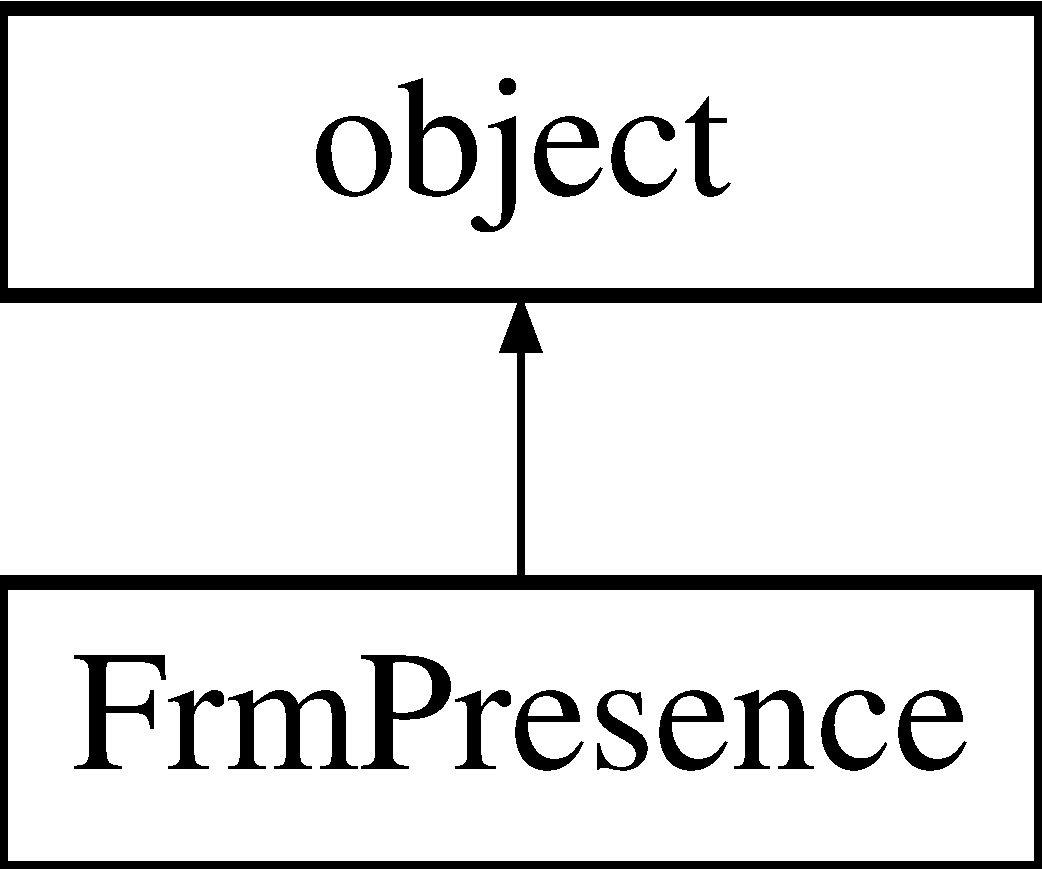
\includegraphics[height=2.000000cm]{class_f_presence_1_1_frm_presence}
\end{center}
\end{figure}
\subsection*{Public Member Functions}
\begin{DoxyCompactItemize}
\item 
\mbox{\Hypertarget{class_f_presence_1_1_frm_presence_a38f4c0a1b0b9f14e89e7670d417e140a}\label{class_f_presence_1_1_frm_presence_a38f4c0a1b0b9f14e89e7670d417e140a}} 
def {\bfseries load} (self, var\+Enabled, show=False)
\item 
\mbox{\Hypertarget{class_f_presence_1_1_frm_presence_ab4f4398c3f210fe4ea6e720401357691}\label{class_f_presence_1_1_frm_presence_ab4f4398c3f210fe4ea6e720401357691}} 
def {\bfseries show} (self)
\item 
\mbox{\Hypertarget{class_f_presence_1_1_frm_presence_adffadd9833af4759460d71b7d00bbf4c}\label{class_f_presence_1_1_frm_presence_adffadd9833af4759460d71b7d00bbf4c}} 
def {\bfseries \+\_\+\+\_\+init\+\_\+\+\_\+} (self, master, parent, enabled=False)
\end{DoxyCompactItemize}
\subsection*{Public Attributes}
\begin{DoxyCompactItemize}
\item 
\mbox{\Hypertarget{class_f_presence_1_1_frm_presence_aa5ba96b8972782a03e3d83def0f965a9}\label{class_f_presence_1_1_frm_presence_aa5ba96b8972782a03e3d83def0f965a9}} 
{\bfseries chk\+Enabled}
\end{DoxyCompactItemize}


\subsection{Detailed Description}


Definition at line 14 of file F\+Presence.\+py.



The documentation for this class was generated from the following file\+:\begin{DoxyCompactItemize}
\item 
F\+Presence.\+py\end{DoxyCompactItemize}

\hypertarget{class_f_run_1_1_frm_run}{}\section{Frm\+Run Class Reference}
\label{class_f_run_1_1_frm_run}\index{Frm\+Run@{Frm\+Run}}
Inheritance diagram for Frm\+Run\+:\begin{figure}[H]
\begin{center}
\leavevmode
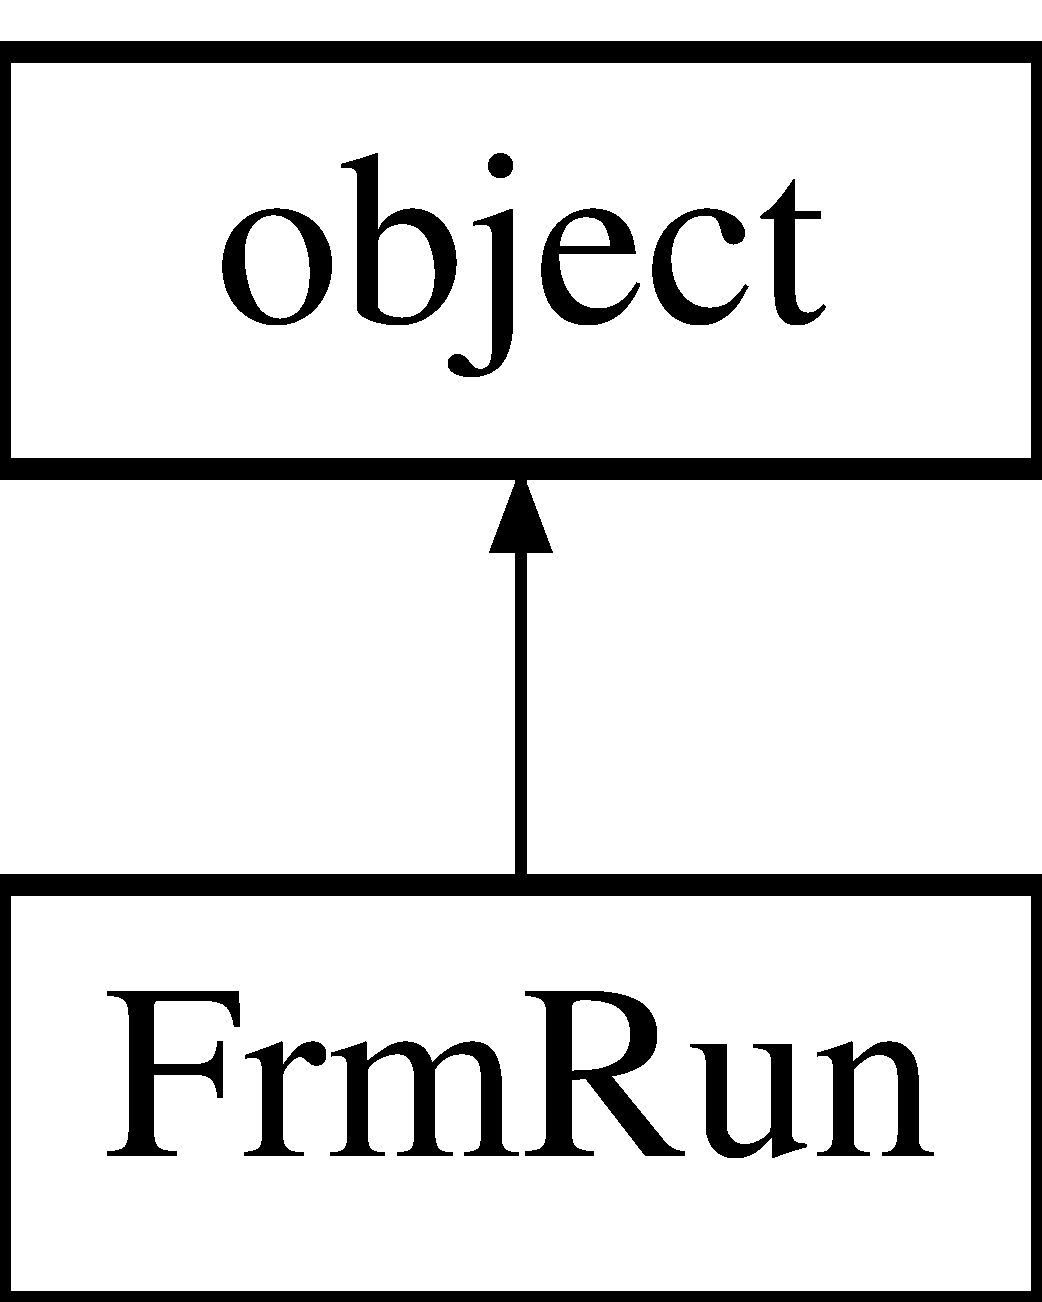
\includegraphics[height=2.000000cm]{class_f_run_1_1_frm_run}
\end{center}
\end{figure}
\subsection*{Public Member Functions}
\begin{DoxyCompactItemize}
\item 
\mbox{\Hypertarget{class_f_run_1_1_frm_run_adb8818239148d2e5c5833a2b062ee9ad}\label{class_f_run_1_1_frm_run_adb8818239148d2e5c5833a2b062ee9ad}} 
def {\bfseries ID} (self)
\item 
\mbox{\Hypertarget{class_f_run_1_1_frm_run_acf44064249ee17c3e8952b4c33512f86}\label{class_f_run_1_1_frm_run_acf44064249ee17c3e8952b4c33512f86}} 
def {\bfseries Frame} (self)
\item 
\mbox{\Hypertarget{class_f_run_1_1_frm_run_a83733e07070207e5d3126c38c9d13b64}\label{class_f_run_1_1_frm_run_a83733e07070207e5d3126c38c9d13b64}} 
def {\bfseries idf\+Filename} (self)
\item 
\mbox{\Hypertarget{class_f_run_1_1_frm_run_a498062a3c3c3e7e027f207deb8b66044}\label{class_f_run_1_1_frm_run_a498062a3c3c3e7e027f207deb8b66044}} 
def {\bfseries weather\+Filename} (self)
\item 
\mbox{\Hypertarget{class_f_run_1_1_frm_run_a2e299137c9278a3e19be8637159b45f2}\label{class_f_run_1_1_frm_run_a2e299137c9278a3e19be8637159b45f2}} 
def {\bfseries output\+Directory} (self)
\item 
\mbox{\Hypertarget{class_f_run_1_1_frm_run_ab3cce165992f522f669dcec287ea44dd}\label{class_f_run_1_1_frm_run_ab3cce165992f522f669dcec287ea44dd}} 
def {\bfseries eplus\+Location} (self)
\item 
\mbox{\Hypertarget{class_f_run_1_1_frm_run_aef9017d108c23a46cf1104cb60008b22}\label{class_f_run_1_1_frm_run_aef9017d108c23a46cf1104cb60008b22}} 
def {\bfseries random\+Window} (self)
\item 
\mbox{\Hypertarget{class_f_run_1_1_frm_run_adf33bbbb399128db1d551e78f27035ff}\label{class_f_run_1_1_frm_run_adf33bbbb399128db1d551e78f27035ff}} 
def {\bfseries random\+Shade} (self)
\item 
\mbox{\Hypertarget{class_f_run_1_1_frm_run_af2a9ec290f7ae7492fe63585812b8183}\label{class_f_run_1_1_frm_run_af2a9ec290f7ae7492fe63585812b8183}} 
def {\bfseries select\+I\+D\+F\+File} (self)
\item 
\mbox{\Hypertarget{class_f_run_1_1_frm_run_a4f5fd238b8fc922831182512cc48cc2a}\label{class_f_run_1_1_frm_run_a4f5fd238b8fc922831182512cc48cc2a}} 
def {\bfseries select\+Weather\+File} (self)
\item 
\mbox{\Hypertarget{class_f_run_1_1_frm_run_a3af7bd47020a22de652781d72c19a265}\label{class_f_run_1_1_frm_run_a3af7bd47020a22de652781d72c19a265}} 
def {\bfseries select\+Output\+Directory} (self)
\item 
\mbox{\Hypertarget{class_f_run_1_1_frm_run_a31bbf949b1276b347fd0ed52a9fd72ef}\label{class_f_run_1_1_frm_run_a31bbf949b1276b347fd0ed52a9fd72ef}} 
def {\bfseries select\+E\+Plus\+Location} (self)
\item 
\mbox{\Hypertarget{class_f_run_1_1_frm_run_ae9dc8d5977a500391665a3caed784f0f}\label{class_f_run_1_1_frm_run_ae9dc8d5977a500391665a3caed784f0f}} 
def {\bfseries output\+File\+Directory\+Exist} (self)
\item 
\mbox{\Hypertarget{class_f_run_1_1_frm_run_a3547c30d307bd52ff9b243f93b306ed3}\label{class_f_run_1_1_frm_run_a3547c30d307bd52ff9b243f93b306ed3}} 
def {\bfseries append\+I\+D\+F\+Addenda} (self, idf\+Filename, p\+Zone\+Names, ep\+Version)
\item 
\mbox{\Hypertarget{class_f_run_1_1_frm_run_a7790f1b9e119c2a171b93bd87222799f}\label{class_f_run_1_1_frm_run_a7790f1b9e119c2a171b93bd87222799f}} 
def {\bfseries create\+Model\+Description} (self, p\+Zone\+Names, ep\+Version)
\item 
\mbox{\Hypertarget{class_f_run_1_1_frm_run_a7170634afdfd97432174a657d775be3c}\label{class_f_run_1_1_frm_run_a7170634afdfd97432174a657d775be3c}} 
def {\bfseries create\+F\+MU} (self, dest, model\+Description\+Filename)
\item 
\mbox{\Hypertarget{class_f_run_1_1_frm_run_a2e67d46dfdc39954a6cd67d45a3b1349}\label{class_f_run_1_1_frm_run_a2e67d46dfdc39954a6cd67d45a3b1349}} 
def {\bfseries copy\+Files\+To\+Simulation\+Folder} (self, session\+Path, dest, config\+Location, model\+Description\+Filename, batch\+Filename)
\item 
\mbox{\Hypertarget{class_f_run_1_1_frm_run_aba02a28f4de8a08e463e224d7d260a9e}\label{class_f_run_1_1_frm_run_aba02a28f4de8a08e463e224d7d260a9e}} 
def {\bfseries get\+Zone\+Lis\+From\+I\+DF} (self)
\item 
\mbox{\Hypertarget{class_f_run_1_1_frm_run_a9b84c203fe51281c386f475a604295d4}\label{class_f_run_1_1_frm_run_a9b84c203fe51281c386f475a604295d4}} 
def {\bfseries get\+Name\+From\+List\+By\+Id} (self, p\+Items, key)
\item 
\mbox{\Hypertarget{class_f_run_1_1_frm_run_accc62f0981c2fe4ae5d75a5f854d6b03}\label{class_f_run_1_1_frm_run_accc62f0981c2fe4ae5d75a5f854d6b03}} 
def {\bfseries compare\+Lists} (self, zones\+I\+DF, zones\+G\+UI)
\item 
\mbox{\Hypertarget{class_f_run_1_1_frm_run_aa625d1a1dcd18fad236a22e1f4372e15}\label{class_f_run_1_1_frm_run_aa625d1a1dcd18fad236a22e1f4372e15}} 
def {\bfseries exec\+E\+Plus\+Simulation\+Sequential} (self, args)
\item 
\mbox{\Hypertarget{class_f_run_1_1_frm_run_a418bf87d2fe3e1eeb0a46cebcc7c6512}\label{class_f_run_1_1_frm_run_a418bf87d2fe3e1eeb0a46cebcc7c6512}} 
def {\bfseries save\+And\+Run} (self)
\end{DoxyCompactItemize}


\subsection{Detailed Description}


Definition at line 41 of file F\+Run.\+py.



The documentation for this class was generated from the following file\+:\begin{DoxyCompactItemize}
\item 
F\+Run.\+py\end{DoxyCompactItemize}

\hypertarget{class_f_shade_1_1_frm_shade}{}\section{Frm\+Shade Class Reference}
\label{class_f_shade_1_1_frm_shade}\index{Frm\+Shade@{Frm\+Shade}}
Inheritance diagram for Frm\+Shade\+:\begin{figure}[H]
\begin{center}
\leavevmode
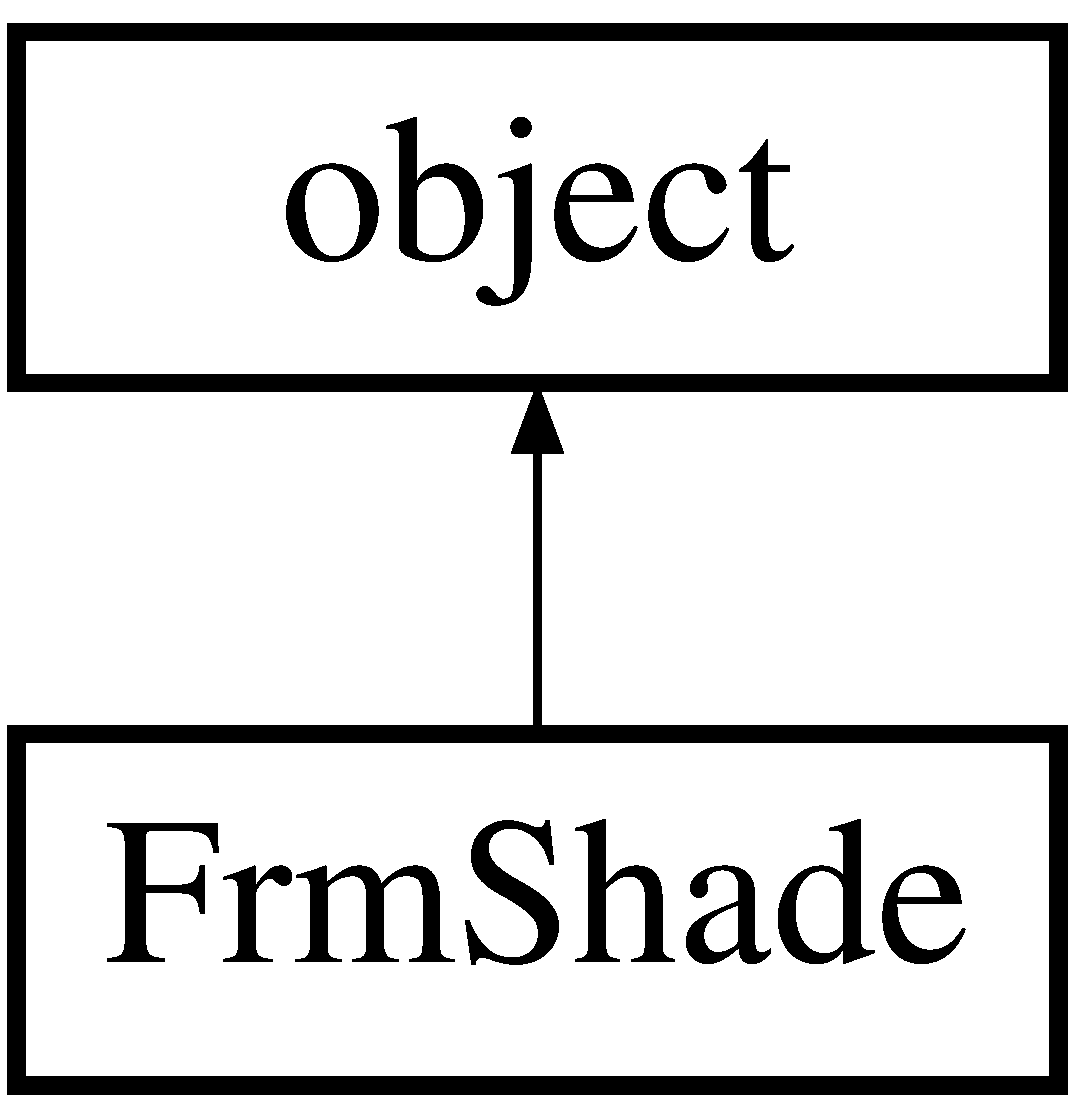
\includegraphics[height=2.000000cm]{class_f_shade_1_1_frm_shade}
\end{center}
\end{figure}
\subsection*{Public Member Functions}
\begin{DoxyCompactItemize}
\item 
\mbox{\Hypertarget{class_f_shade_1_1_frm_shade_abf03882231e5ddb36fa60b96c5001cd2}\label{class_f_shade_1_1_frm_shade_abf03882231e5ddb36fa60b96c5001cd2}} 
def {\bfseries load} (self, id=0, name=\textquotesingle{}\textquotesingle{}, a01arr=0, b01inarr=0, b01sarr=0, a10arr=0, b10inarr=0, b10sarr=0, a01int=0, b01inint=0, b01sint=0, a10int=0, b10inint=0, b10sint=0, afullraise=0, boutfullraise=0, bsfullraise=0, bsfulllower=0, boutfulllower=0, afulllower=0, a\+S\+Flower=0, b\+S\+Flower=0, shapelower=0, show=False)
\item 
\mbox{\Hypertarget{class_f_shade_1_1_frm_shade_ab4f4398c3f210fe4ea6e720401357691}\label{class_f_shade_1_1_frm_shade_ab4f4398c3f210fe4ea6e720401357691}} 
def {\bfseries show} (self)
\item 
\mbox{\Hypertarget{class_f_shade_1_1_frm_shade_a2a7c017b71cb1ea5efc601d706ffb5d2}\label{class_f_shade_1_1_frm_shade_a2a7c017b71cb1ea5efc601d706ffb5d2}} 
def {\bfseries \+\_\+\+\_\+init\+\_\+\+\_\+} (self, master, parent, id=0, name=\textquotesingle{}\textquotesingle{}, a01arr=0, b01inarr=0, b01sarr=0, a10arr=0, b10inarr=0, b10sarr=0, a01int=0, b01inint=0, b01sint=0, a10int=0, b10inint=0, b10sint=0, afullraise=0, boutfullraise=0, bsfullraise=0, bsfulllower=0, boutfulllower=0, afulllower=0, a\+S\+Flower=0, b\+S\+Flower=0, shapelower=0)
\end{DoxyCompactItemize}
\subsection*{Public Attributes}
\begin{DoxyCompactItemize}
\item 
\mbox{\Hypertarget{class_f_shade_1_1_frm_shade_aa6bd44217fd47f4f9adc0ad55b39a129}\label{class_f_shade_1_1_frm_shade_aa6bd44217fd47f4f9adc0ad55b39a129}} 
{\bfseries lblid}
\item 
\mbox{\Hypertarget{class_f_shade_1_1_frm_shade_a3479be45da7e409c64ec5f438bc06777}\label{class_f_shade_1_1_frm_shade_a3479be45da7e409c64ec5f438bc06777}} 
{\bfseries txtid}
\item 
\mbox{\Hypertarget{class_f_shade_1_1_frm_shade_afe9b98e5038ae1c69e5bb7eef0ed7cc4}\label{class_f_shade_1_1_frm_shade_afe9b98e5038ae1c69e5bb7eef0ed7cc4}} 
{\bfseries lblname}
\item 
\mbox{\Hypertarget{class_f_shade_1_1_frm_shade_a24025fc9f698a9db8fb4f3c1c3c32e40}\label{class_f_shade_1_1_frm_shade_a24025fc9f698a9db8fb4f3c1c3c32e40}} 
{\bfseries txtname}
\item 
\mbox{\Hypertarget{class_f_shade_1_1_frm_shade_a2caf77b2db014c42ebbb42d05da6ed62}\label{class_f_shade_1_1_frm_shade_a2caf77b2db014c42ebbb42d05da6ed62}} 
{\bfseries lbla01arr}
\item 
\mbox{\Hypertarget{class_f_shade_1_1_frm_shade_a18533ee8afd9bd8f2941b8fa0beccebc}\label{class_f_shade_1_1_frm_shade_a18533ee8afd9bd8f2941b8fa0beccebc}} 
{\bfseries txta01arr}
\item 
\mbox{\Hypertarget{class_f_shade_1_1_frm_shade_a0eeb45dca5905245239d26d276ea519d}\label{class_f_shade_1_1_frm_shade_a0eeb45dca5905245239d26d276ea519d}} 
{\bfseries lblb01inarr}
\item 
\mbox{\Hypertarget{class_f_shade_1_1_frm_shade_a1a2fbb1a55d1a5cc381eda8a14e04458}\label{class_f_shade_1_1_frm_shade_a1a2fbb1a55d1a5cc381eda8a14e04458}} 
{\bfseries txtb01inarr}
\item 
\mbox{\Hypertarget{class_f_shade_1_1_frm_shade_a276024a1709de10b09cff60305b10128}\label{class_f_shade_1_1_frm_shade_a276024a1709de10b09cff60305b10128}} 
{\bfseries lblb01sarr}
\item 
\mbox{\Hypertarget{class_f_shade_1_1_frm_shade_a4d3bc1ae16990fe668609d8bf0205339}\label{class_f_shade_1_1_frm_shade_a4d3bc1ae16990fe668609d8bf0205339}} 
{\bfseries txtb01sarr}
\item 
\mbox{\Hypertarget{class_f_shade_1_1_frm_shade_a867070d964d82813fcac2ef2b3b077ed}\label{class_f_shade_1_1_frm_shade_a867070d964d82813fcac2ef2b3b077ed}} 
{\bfseries lbla10arr}
\item 
\mbox{\Hypertarget{class_f_shade_1_1_frm_shade_a4392ed9c9867f360162536707774f330}\label{class_f_shade_1_1_frm_shade_a4392ed9c9867f360162536707774f330}} 
{\bfseries txta10arr}
\item 
\mbox{\Hypertarget{class_f_shade_1_1_frm_shade_a38513e68850590624df6a4cf8811eb05}\label{class_f_shade_1_1_frm_shade_a38513e68850590624df6a4cf8811eb05}} 
{\bfseries lblb10inarr}
\item 
\mbox{\Hypertarget{class_f_shade_1_1_frm_shade_afba4579fbdfd788ba34e9198b85a17b7}\label{class_f_shade_1_1_frm_shade_afba4579fbdfd788ba34e9198b85a17b7}} 
{\bfseries txtb10inarr}
\item 
\mbox{\Hypertarget{class_f_shade_1_1_frm_shade_a692e9ec15f0730c5262120b25613f464}\label{class_f_shade_1_1_frm_shade_a692e9ec15f0730c5262120b25613f464}} 
{\bfseries lblb10sarr}
\item 
\mbox{\Hypertarget{class_f_shade_1_1_frm_shade_a2d0050a2be757052f0bf482f3f3b9588}\label{class_f_shade_1_1_frm_shade_a2d0050a2be757052f0bf482f3f3b9588}} 
{\bfseries txtb10sarr}
\item 
\mbox{\Hypertarget{class_f_shade_1_1_frm_shade_a9be0e421ec402a0525188faeef4d97e2}\label{class_f_shade_1_1_frm_shade_a9be0e421ec402a0525188faeef4d97e2}} 
{\bfseries lbla01int}
\item 
\mbox{\Hypertarget{class_f_shade_1_1_frm_shade_a53317edd6ad050f1180a1e4805257c49}\label{class_f_shade_1_1_frm_shade_a53317edd6ad050f1180a1e4805257c49}} 
{\bfseries txta01int}
\item 
\mbox{\Hypertarget{class_f_shade_1_1_frm_shade_a46802499cb7bdd5b657101eaecbf567e}\label{class_f_shade_1_1_frm_shade_a46802499cb7bdd5b657101eaecbf567e}} 
{\bfseries lblb01inint}
\item 
\mbox{\Hypertarget{class_f_shade_1_1_frm_shade_a929c0afda74329360adc1b84cc7946c5}\label{class_f_shade_1_1_frm_shade_a929c0afda74329360adc1b84cc7946c5}} 
{\bfseries txtb01inint}
\item 
\mbox{\Hypertarget{class_f_shade_1_1_frm_shade_a3b44a26db63580f821990a4fa49d7255}\label{class_f_shade_1_1_frm_shade_a3b44a26db63580f821990a4fa49d7255}} 
{\bfseries lblb01sint}
\item 
\mbox{\Hypertarget{class_f_shade_1_1_frm_shade_a674b086a6711cb9435f9578275e8aecd}\label{class_f_shade_1_1_frm_shade_a674b086a6711cb9435f9578275e8aecd}} 
{\bfseries txtb01sint}
\item 
\mbox{\Hypertarget{class_f_shade_1_1_frm_shade_ae467c58aec316f606ce91b2ce5488893}\label{class_f_shade_1_1_frm_shade_ae467c58aec316f606ce91b2ce5488893}} 
{\bfseries lbla10int}
\item 
\mbox{\Hypertarget{class_f_shade_1_1_frm_shade_a01fa0a51a9053a98121d84828c19136b}\label{class_f_shade_1_1_frm_shade_a01fa0a51a9053a98121d84828c19136b}} 
{\bfseries txta10int}
\item 
\mbox{\Hypertarget{class_f_shade_1_1_frm_shade_a8220503d6720abce9a85d2c2c3b01531}\label{class_f_shade_1_1_frm_shade_a8220503d6720abce9a85d2c2c3b01531}} 
{\bfseries lblb10inint}
\item 
\mbox{\Hypertarget{class_f_shade_1_1_frm_shade_aaf5b8450e441fdaae28a8367a95b287d}\label{class_f_shade_1_1_frm_shade_aaf5b8450e441fdaae28a8367a95b287d}} 
{\bfseries txtb10inint}
\item 
\mbox{\Hypertarget{class_f_shade_1_1_frm_shade_acfe38793a40287d684278fcb19368177}\label{class_f_shade_1_1_frm_shade_acfe38793a40287d684278fcb19368177}} 
{\bfseries lblb10sint}
\item 
\mbox{\Hypertarget{class_f_shade_1_1_frm_shade_ae12d55b0a6903dc757a7bfa1efa880b5}\label{class_f_shade_1_1_frm_shade_ae12d55b0a6903dc757a7bfa1efa880b5}} 
{\bfseries txtb10sint}
\item 
\mbox{\Hypertarget{class_f_shade_1_1_frm_shade_a946190b1443c0d9f0ffe53c16a218cf9}\label{class_f_shade_1_1_frm_shade_a946190b1443c0d9f0ffe53c16a218cf9}} 
{\bfseries lblafullraise}
\item 
\mbox{\Hypertarget{class_f_shade_1_1_frm_shade_ad9a1634590367224ab16ccd1718df598}\label{class_f_shade_1_1_frm_shade_ad9a1634590367224ab16ccd1718df598}} 
{\bfseries txtafullraise}
\item 
\mbox{\Hypertarget{class_f_shade_1_1_frm_shade_aac7c6d95b7b6145ae57123492fdb00bb}\label{class_f_shade_1_1_frm_shade_aac7c6d95b7b6145ae57123492fdb00bb}} 
{\bfseries lblboutfullraise}
\item 
\mbox{\Hypertarget{class_f_shade_1_1_frm_shade_ab942f3f1e6cff2fff06892ca07834abf}\label{class_f_shade_1_1_frm_shade_ab942f3f1e6cff2fff06892ca07834abf}} 
{\bfseries txtboutfullraise}
\item 
\mbox{\Hypertarget{class_f_shade_1_1_frm_shade_a30a32c1f85bb74b2fef4c26c1714b2ba}\label{class_f_shade_1_1_frm_shade_a30a32c1f85bb74b2fef4c26c1714b2ba}} 
{\bfseries lblbsfullraise}
\item 
\mbox{\Hypertarget{class_f_shade_1_1_frm_shade_a912c0359e2fe8e182f17c6f97f8f2a05}\label{class_f_shade_1_1_frm_shade_a912c0359e2fe8e182f17c6f97f8f2a05}} 
{\bfseries txtbsfullraise}
\item 
\mbox{\Hypertarget{class_f_shade_1_1_frm_shade_a9842f7725d77ea6eee67ecc15117029e}\label{class_f_shade_1_1_frm_shade_a9842f7725d77ea6eee67ecc15117029e}} 
{\bfseries lblbsfulllower}
\item 
\mbox{\Hypertarget{class_f_shade_1_1_frm_shade_a533912d2ffc48d1032c6209f46443691}\label{class_f_shade_1_1_frm_shade_a533912d2ffc48d1032c6209f46443691}} 
{\bfseries txtbsfulllower}
\item 
\mbox{\Hypertarget{class_f_shade_1_1_frm_shade_a9bfd57c389c6674fbc30ac2949475b26}\label{class_f_shade_1_1_frm_shade_a9bfd57c389c6674fbc30ac2949475b26}} 
{\bfseries lblboutfulllower}
\item 
\mbox{\Hypertarget{class_f_shade_1_1_frm_shade_afbd4ad837e08f465822e6daf709033d1}\label{class_f_shade_1_1_frm_shade_afbd4ad837e08f465822e6daf709033d1}} 
{\bfseries txtboutfulllower}
\item 
\mbox{\Hypertarget{class_f_shade_1_1_frm_shade_ad8f1f0ede6997aedf1c65790fd878abc}\label{class_f_shade_1_1_frm_shade_ad8f1f0ede6997aedf1c65790fd878abc}} 
{\bfseries lblafulllower}
\item 
\mbox{\Hypertarget{class_f_shade_1_1_frm_shade_ac8623e08c5f993fd4ea02e356b56d8bc}\label{class_f_shade_1_1_frm_shade_ac8623e08c5f993fd4ea02e356b56d8bc}} 
{\bfseries txtafulllower}
\item 
\mbox{\Hypertarget{class_f_shade_1_1_frm_shade_aabb6c3a46372acf83ce076aa7577cd5e}\label{class_f_shade_1_1_frm_shade_aabb6c3a46372acf83ce076aa7577cd5e}} 
{\bfseries lbla\+S\+Flower}
\item 
\mbox{\Hypertarget{class_f_shade_1_1_frm_shade_ac202e29870e8a2f3d4c1aa9c8d781cfa}\label{class_f_shade_1_1_frm_shade_ac202e29870e8a2f3d4c1aa9c8d781cfa}} 
{\bfseries txta\+S\+Flower}
\item 
\mbox{\Hypertarget{class_f_shade_1_1_frm_shade_a49c287b75ce07b9c1ee0001cdde3daab}\label{class_f_shade_1_1_frm_shade_a49c287b75ce07b9c1ee0001cdde3daab}} 
{\bfseries lblb\+S\+Flower}
\item 
\mbox{\Hypertarget{class_f_shade_1_1_frm_shade_a6d8190aee3f7bf23eb54ca69468cd180}\label{class_f_shade_1_1_frm_shade_a6d8190aee3f7bf23eb54ca69468cd180}} 
{\bfseries txtb\+S\+Flower}
\item 
\mbox{\Hypertarget{class_f_shade_1_1_frm_shade_ad5b055829b82a32cc5fc153fa22a1b6a}\label{class_f_shade_1_1_frm_shade_ad5b055829b82a32cc5fc153fa22a1b6a}} 
{\bfseries lblshapelower}
\item 
\mbox{\Hypertarget{class_f_shade_1_1_frm_shade_a0d43e851d8ceaaa1c7ed178234cdaa6a}\label{class_f_shade_1_1_frm_shade_a0d43e851d8ceaaa1c7ed178234cdaa6a}} 
{\bfseries txtshapelower}
\end{DoxyCompactItemize}


\subsection{Detailed Description}


Definition at line 14 of file F\+Shade.\+py.



The documentation for this class was generated from the following file\+:\begin{DoxyCompactItemize}
\item 
F\+Shade.\+py\end{DoxyCompactItemize}

\hypertarget{class_f_shades_1_1_frm_shades}{}\section{Frm\+Shades Class Reference}
\label{class_f_shades_1_1_frm_shades}\index{Frm\+Shades@{Frm\+Shades}}
Inheritance diagram for Frm\+Shades\+:\begin{figure}[H]
\begin{center}
\leavevmode
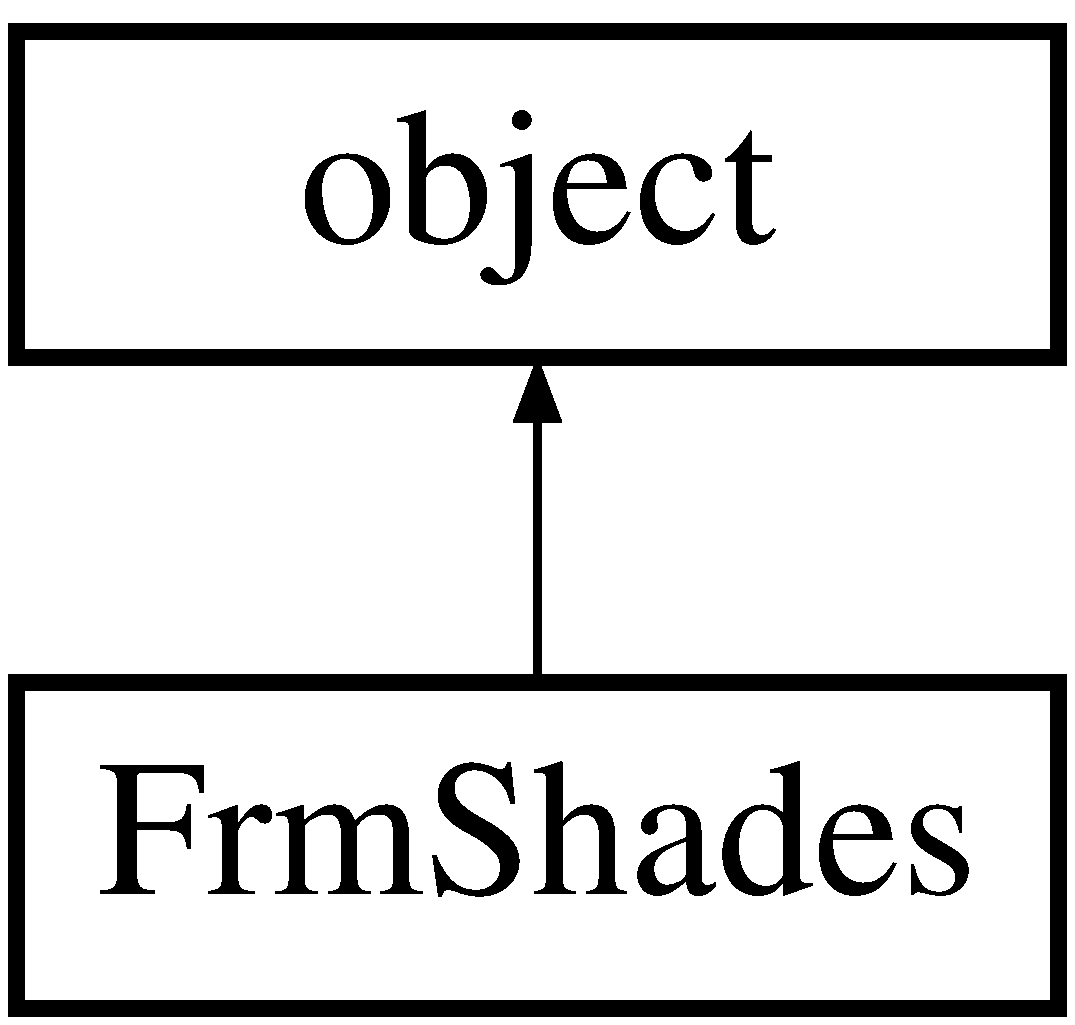
\includegraphics[height=2.000000cm]{class_f_shades_1_1_frm_shades}
\end{center}
\end{figure}
\subsection*{Public Member Functions}
\begin{DoxyCompactItemize}
\item 
\mbox{\Hypertarget{class_f_shades_1_1_frm_shades_a38f4c0a1b0b9f14e89e7670d417e140a}\label{class_f_shades_1_1_frm_shades_a38f4c0a1b0b9f14e89e7670d417e140a}} 
def {\bfseries load} (self, var\+Enabled, show=False)
\item 
\mbox{\Hypertarget{class_f_shades_1_1_frm_shades_ab4f4398c3f210fe4ea6e720401357691}\label{class_f_shades_1_1_frm_shades_ab4f4398c3f210fe4ea6e720401357691}} 
def {\bfseries show} (self)
\item 
\mbox{\Hypertarget{class_f_shades_1_1_frm_shades_adffadd9833af4759460d71b7d00bbf4c}\label{class_f_shades_1_1_frm_shades_adffadd9833af4759460d71b7d00bbf4c}} 
def {\bfseries \+\_\+\+\_\+init\+\_\+\+\_\+} (self, master, parent, enabled=False)
\end{DoxyCompactItemize}
\subsection*{Public Attributes}
\begin{DoxyCompactItemize}
\item 
\mbox{\Hypertarget{class_f_shades_1_1_frm_shades_aa5ba96b8972782a03e3d83def0f965a9}\label{class_f_shades_1_1_frm_shades_aa5ba96b8972782a03e3d83def0f965a9}} 
{\bfseries chk\+Enabled}
\end{DoxyCompactItemize}


\subsection{Detailed Description}


Definition at line 14 of file F\+Shades.\+py.



The documentation for this class was generated from the following file\+:\begin{DoxyCompactItemize}
\item 
F\+Shades.\+py\end{DoxyCompactItemize}

\hypertarget{class_f_window_1_1_frm_window}{}\section{Frm\+Window Class Reference}
\label{class_f_window_1_1_frm_window}\index{Frm\+Window@{Frm\+Window}}
Inheritance diagram for Frm\+Window\+:\begin{figure}[H]
\begin{center}
\leavevmode
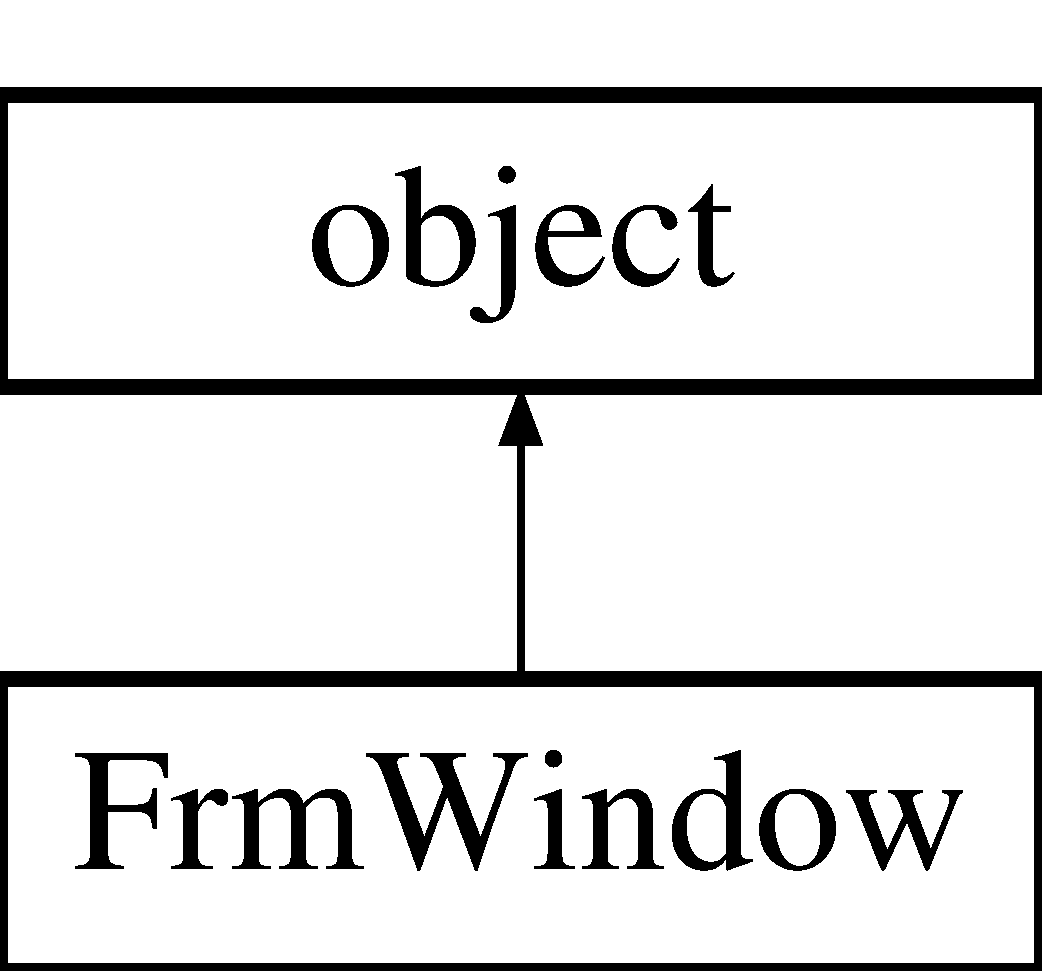
\includegraphics[height=2.000000cm]{class_f_window_1_1_frm_window}
\end{center}
\end{figure}
\subsection*{Public Member Functions}
\begin{DoxyCompactItemize}
\item 
\mbox{\Hypertarget{class_f_window_1_1_frm_window_ae349def881aefeb65ebff931d052d0cd}\label{class_f_window_1_1_frm_window_ae349def881aefeb65ebff931d052d0cd}} 
def {\bfseries load} (self, id=None, name=None, aop=None, bopout=None, shapeop=None, a01arr=None, b01inarr=None, b01outarr=None, b01absprevarr=None, b01rnarr=None, a01int=None, b01inint=None, b01outint=None, b01presint=None, b01rnint=None, a01dep=None, b01outdep=None, b01absdep=None, b01gddep=None, a10dep=None, b10indep=None, b10outdep=None, b10absdep=None, b10gddep=None, show=False)
\item 
\mbox{\Hypertarget{class_f_window_1_1_frm_window_ab4f4398c3f210fe4ea6e720401357691}\label{class_f_window_1_1_frm_window_ab4f4398c3f210fe4ea6e720401357691}} 
def {\bfseries show} (self)
\item 
\mbox{\Hypertarget{class_f_window_1_1_frm_window_a372b8cd7a25c46644ad20ca45547451c}\label{class_f_window_1_1_frm_window_a372b8cd7a25c46644ad20ca45547451c}} 
def {\bfseries \+\_\+\+\_\+init\+\_\+\+\_\+} (self, master, parent, id=0, name=\textquotesingle{}\textquotesingle{}, aop=0, bopout=0, shapeop=0, a01arr=0, b01inarr=0, b01outarr=0, b01absprevarr=0, b01rnarr=0, a01int=0, b01inint=0, b01outint=0, b01presint=0, b01rnint=0, a01dep=0, b01outdep=0, b01absdep=0, b01gddep=0, a10dep=0, b10indep=0, b10outdep=0, b10absdep=0, b10gddep=0)
\end{DoxyCompactItemize}
\subsection*{Public Attributes}
\begin{DoxyCompactItemize}
\item 
\mbox{\Hypertarget{class_f_window_1_1_frm_window_aa6bd44217fd47f4f9adc0ad55b39a129}\label{class_f_window_1_1_frm_window_aa6bd44217fd47f4f9adc0ad55b39a129}} 
{\bfseries lblid}
\item 
\mbox{\Hypertarget{class_f_window_1_1_frm_window_a3479be45da7e409c64ec5f438bc06777}\label{class_f_window_1_1_frm_window_a3479be45da7e409c64ec5f438bc06777}} 
{\bfseries txtid}
\item 
\mbox{\Hypertarget{class_f_window_1_1_frm_window_afe9b98e5038ae1c69e5bb7eef0ed7cc4}\label{class_f_window_1_1_frm_window_afe9b98e5038ae1c69e5bb7eef0ed7cc4}} 
{\bfseries lblname}
\item 
\mbox{\Hypertarget{class_f_window_1_1_frm_window_a24025fc9f698a9db8fb4f3c1c3c32e40}\label{class_f_window_1_1_frm_window_a24025fc9f698a9db8fb4f3c1c3c32e40}} 
{\bfseries txtname}
\item 
\mbox{\Hypertarget{class_f_window_1_1_frm_window_a202b9e4000925afd11dd3778f8e3d53b}\label{class_f_window_1_1_frm_window_a202b9e4000925afd11dd3778f8e3d53b}} 
{\bfseries lblaop}
\item 
\mbox{\Hypertarget{class_f_window_1_1_frm_window_a3d29d1e339b89708e801a531f5f83a59}\label{class_f_window_1_1_frm_window_a3d29d1e339b89708e801a531f5f83a59}} 
{\bfseries txtaop}
\item 
\mbox{\Hypertarget{class_f_window_1_1_frm_window_a480a59fbfa037e0c89ad0ca02fbf4738}\label{class_f_window_1_1_frm_window_a480a59fbfa037e0c89ad0ca02fbf4738}} 
{\bfseries lblbopout}
\item 
\mbox{\Hypertarget{class_f_window_1_1_frm_window_a137954e3fd91166990e18167b994c312}\label{class_f_window_1_1_frm_window_a137954e3fd91166990e18167b994c312}} 
{\bfseries txtbopout}
\item 
\mbox{\Hypertarget{class_f_window_1_1_frm_window_a9a4f4c46875959e0d7a7515f3c28afbd}\label{class_f_window_1_1_frm_window_a9a4f4c46875959e0d7a7515f3c28afbd}} 
{\bfseries lblshapeop}
\item 
\mbox{\Hypertarget{class_f_window_1_1_frm_window_a16cef3053a1a0f1a07acfacd69a82e80}\label{class_f_window_1_1_frm_window_a16cef3053a1a0f1a07acfacd69a82e80}} 
{\bfseries txtshapeop}
\item 
\mbox{\Hypertarget{class_f_window_1_1_frm_window_a2caf77b2db014c42ebbb42d05da6ed62}\label{class_f_window_1_1_frm_window_a2caf77b2db014c42ebbb42d05da6ed62}} 
{\bfseries lbla01arr}
\item 
\mbox{\Hypertarget{class_f_window_1_1_frm_window_a18533ee8afd9bd8f2941b8fa0beccebc}\label{class_f_window_1_1_frm_window_a18533ee8afd9bd8f2941b8fa0beccebc}} 
{\bfseries txta01arr}
\item 
\mbox{\Hypertarget{class_f_window_1_1_frm_window_a0eeb45dca5905245239d26d276ea519d}\label{class_f_window_1_1_frm_window_a0eeb45dca5905245239d26d276ea519d}} 
{\bfseries lblb01inarr}
\item 
\mbox{\Hypertarget{class_f_window_1_1_frm_window_a1a2fbb1a55d1a5cc381eda8a14e04458}\label{class_f_window_1_1_frm_window_a1a2fbb1a55d1a5cc381eda8a14e04458}} 
{\bfseries txtb01inarr}
\item 
\mbox{\Hypertarget{class_f_window_1_1_frm_window_a52ba210952bc01f0e1f1132912ef8fad}\label{class_f_window_1_1_frm_window_a52ba210952bc01f0e1f1132912ef8fad}} 
{\bfseries lblb01outarr}
\item 
\mbox{\Hypertarget{class_f_window_1_1_frm_window_ad63477401d53203d94be74453d522c5e}\label{class_f_window_1_1_frm_window_ad63477401d53203d94be74453d522c5e}} 
{\bfseries txtb01outarr}
\item 
\mbox{\Hypertarget{class_f_window_1_1_frm_window_a4c1183ea9069f51fd4f8d45ff788de2e}\label{class_f_window_1_1_frm_window_a4c1183ea9069f51fd4f8d45ff788de2e}} 
{\bfseries lblb01absprevarr}
\item 
\mbox{\Hypertarget{class_f_window_1_1_frm_window_ae1aea005005ac91d3f369724499fc277}\label{class_f_window_1_1_frm_window_ae1aea005005ac91d3f369724499fc277}} 
{\bfseries txtb01absprevarr}
\item 
\mbox{\Hypertarget{class_f_window_1_1_frm_window_a3a6f6161bac5b5bc11497a9d6e59cae0}\label{class_f_window_1_1_frm_window_a3a6f6161bac5b5bc11497a9d6e59cae0}} 
{\bfseries lblb01rnarr}
\item 
\mbox{\Hypertarget{class_f_window_1_1_frm_window_aa2fe162ceb2f9ffb1d677d84d8731807}\label{class_f_window_1_1_frm_window_aa2fe162ceb2f9ffb1d677d84d8731807}} 
{\bfseries txtb01rnarr}
\item 
\mbox{\Hypertarget{class_f_window_1_1_frm_window_a9be0e421ec402a0525188faeef4d97e2}\label{class_f_window_1_1_frm_window_a9be0e421ec402a0525188faeef4d97e2}} 
{\bfseries lbla01int}
\item 
\mbox{\Hypertarget{class_f_window_1_1_frm_window_a53317edd6ad050f1180a1e4805257c49}\label{class_f_window_1_1_frm_window_a53317edd6ad050f1180a1e4805257c49}} 
{\bfseries txta01int}
\item 
\mbox{\Hypertarget{class_f_window_1_1_frm_window_a46802499cb7bdd5b657101eaecbf567e}\label{class_f_window_1_1_frm_window_a46802499cb7bdd5b657101eaecbf567e}} 
{\bfseries lblb01inint}
\item 
\mbox{\Hypertarget{class_f_window_1_1_frm_window_a929c0afda74329360adc1b84cc7946c5}\label{class_f_window_1_1_frm_window_a929c0afda74329360adc1b84cc7946c5}} 
{\bfseries txtb01inint}
\item 
\mbox{\Hypertarget{class_f_window_1_1_frm_window_a28962865c013827903e2958c5679fbc8}\label{class_f_window_1_1_frm_window_a28962865c013827903e2958c5679fbc8}} 
{\bfseries lblb01outint}
\item 
\mbox{\Hypertarget{class_f_window_1_1_frm_window_a2fadd3d9ef9d18d316280449371e45b7}\label{class_f_window_1_1_frm_window_a2fadd3d9ef9d18d316280449371e45b7}} 
{\bfseries txtb01outint}
\item 
\mbox{\Hypertarget{class_f_window_1_1_frm_window_aa65344e3fdd5d9ae8e8eeb0fb77e7cff}\label{class_f_window_1_1_frm_window_aa65344e3fdd5d9ae8e8eeb0fb77e7cff}} 
{\bfseries lblb01presint}
\item 
\mbox{\Hypertarget{class_f_window_1_1_frm_window_afd4c7c7d7d94ffdcc2d66f525c4abe43}\label{class_f_window_1_1_frm_window_afd4c7c7d7d94ffdcc2d66f525c4abe43}} 
{\bfseries txtb01presint}
\item 
\mbox{\Hypertarget{class_f_window_1_1_frm_window_a83eab093994f913fda7586be8977c149}\label{class_f_window_1_1_frm_window_a83eab093994f913fda7586be8977c149}} 
{\bfseries lblb01rnint}
\item 
\mbox{\Hypertarget{class_f_window_1_1_frm_window_ac3e565e497f28043013903e6ae0b06b3}\label{class_f_window_1_1_frm_window_ac3e565e497f28043013903e6ae0b06b3}} 
{\bfseries txtb01rnint}
\item 
\mbox{\Hypertarget{class_f_window_1_1_frm_window_a53c12344aed3beba709baf4e38532b7a}\label{class_f_window_1_1_frm_window_a53c12344aed3beba709baf4e38532b7a}} 
{\bfseries lbla01dep}
\item 
\mbox{\Hypertarget{class_f_window_1_1_frm_window_a697c42d0c41a2f8c36d54d2c10ba8c88}\label{class_f_window_1_1_frm_window_a697c42d0c41a2f8c36d54d2c10ba8c88}} 
{\bfseries txta01dep}
\item 
\mbox{\Hypertarget{class_f_window_1_1_frm_window_a22bd829f66ce02260ba540b595401801}\label{class_f_window_1_1_frm_window_a22bd829f66ce02260ba540b595401801}} 
{\bfseries lblb01outdep}
\item 
\mbox{\Hypertarget{class_f_window_1_1_frm_window_a31c982baaf1b352a5851fd0833b04e46}\label{class_f_window_1_1_frm_window_a31c982baaf1b352a5851fd0833b04e46}} 
{\bfseries txtb01outdep}
\item 
\mbox{\Hypertarget{class_f_window_1_1_frm_window_a39b3bdd84b541d15dd6daac2a925221c}\label{class_f_window_1_1_frm_window_a39b3bdd84b541d15dd6daac2a925221c}} 
{\bfseries lblb01absdep}
\item 
\mbox{\Hypertarget{class_f_window_1_1_frm_window_a179785c9633f5b0a87e6bb43d0f31f8e}\label{class_f_window_1_1_frm_window_a179785c9633f5b0a87e6bb43d0f31f8e}} 
{\bfseries txtb01absdep}
\item 
\mbox{\Hypertarget{class_f_window_1_1_frm_window_ab3896e6fb4384e2848dd6bf09373409b}\label{class_f_window_1_1_frm_window_ab3896e6fb4384e2848dd6bf09373409b}} 
{\bfseries lblb01gddep}
\item 
\mbox{\Hypertarget{class_f_window_1_1_frm_window_af8633ffbf58b44edc3401c21fdb5ca6d}\label{class_f_window_1_1_frm_window_af8633ffbf58b44edc3401c21fdb5ca6d}} 
{\bfseries txtb01gddep}
\item 
\mbox{\Hypertarget{class_f_window_1_1_frm_window_a5d7aac514a3b3adc4a5ba5187b1d617f}\label{class_f_window_1_1_frm_window_a5d7aac514a3b3adc4a5ba5187b1d617f}} 
{\bfseries lbla10dep}
\item 
\mbox{\Hypertarget{class_f_window_1_1_frm_window_ae037cd161cef380b0d4811cb67640df4}\label{class_f_window_1_1_frm_window_ae037cd161cef380b0d4811cb67640df4}} 
{\bfseries txta10dep}
\item 
\mbox{\Hypertarget{class_f_window_1_1_frm_window_a7a5f5014b942c34d60557e803b6c7d21}\label{class_f_window_1_1_frm_window_a7a5f5014b942c34d60557e803b6c7d21}} 
{\bfseries lblb10indep}
\item 
\mbox{\Hypertarget{class_f_window_1_1_frm_window_ac6f0a0ff9327c17b25e9169d5ca1dc8c}\label{class_f_window_1_1_frm_window_ac6f0a0ff9327c17b25e9169d5ca1dc8c}} 
{\bfseries txtb10indep}
\item 
\mbox{\Hypertarget{class_f_window_1_1_frm_window_a088d51a5e06c2b3895b13ef870f9e5c0}\label{class_f_window_1_1_frm_window_a088d51a5e06c2b3895b13ef870f9e5c0}} 
{\bfseries lblb10outdep}
\item 
\mbox{\Hypertarget{class_f_window_1_1_frm_window_a78a4ef4b237ff02a542a2468e10d4721}\label{class_f_window_1_1_frm_window_a78a4ef4b237ff02a542a2468e10d4721}} 
{\bfseries txtb10outdep}
\item 
\mbox{\Hypertarget{class_f_window_1_1_frm_window_a40c04d65555fb43215e446e3ffe0204e}\label{class_f_window_1_1_frm_window_a40c04d65555fb43215e446e3ffe0204e}} 
{\bfseries lblb10absdep}
\item 
\mbox{\Hypertarget{class_f_window_1_1_frm_window_a0cd6f3026287779daafcb415d3a27bb8}\label{class_f_window_1_1_frm_window_a0cd6f3026287779daafcb415d3a27bb8}} 
{\bfseries txtb10absdep}
\item 
\mbox{\Hypertarget{class_f_window_1_1_frm_window_a4e7c498d414c44594c409f928ac7cd5f}\label{class_f_window_1_1_frm_window_a4e7c498d414c44594c409f928ac7cd5f}} 
{\bfseries lblb10gddep}
\item 
\mbox{\Hypertarget{class_f_window_1_1_frm_window_a682eda02aac30e3a8553f093cbb54f29}\label{class_f_window_1_1_frm_window_a682eda02aac30e3a8553f093cbb54f29}} 
{\bfseries txtb10gddep}
\end{DoxyCompactItemize}


\subsection{Detailed Description}


Definition at line 14 of file F\+Window.\+py.



The documentation for this class was generated from the following file\+:\begin{DoxyCompactItemize}
\item 
F\+Window.\+py\end{DoxyCompactItemize}

\hypertarget{class_f_windows_1_1_frm_windows}{}\section{Frm\+Windows Class Reference}
\label{class_f_windows_1_1_frm_windows}\index{Frm\+Windows@{Frm\+Windows}}
Inheritance diagram for Frm\+Windows\+:\begin{figure}[H]
\begin{center}
\leavevmode
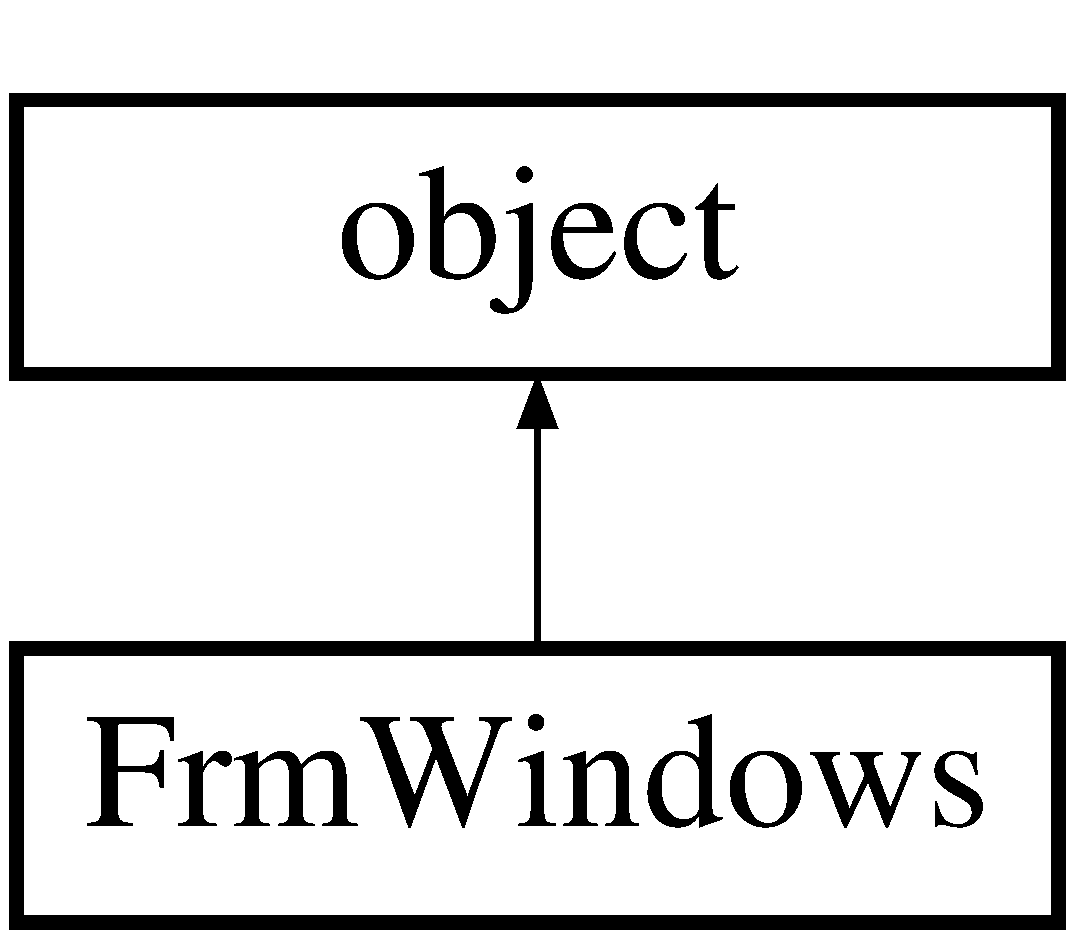
\includegraphics[height=2.000000cm]{class_f_windows_1_1_frm_windows}
\end{center}
\end{figure}
\subsection*{Public Member Functions}
\begin{DoxyCompactItemize}
\item 
\mbox{\Hypertarget{class_f_windows_1_1_frm_windows_a38f4c0a1b0b9f14e89e7670d417e140a}\label{class_f_windows_1_1_frm_windows_a38f4c0a1b0b9f14e89e7670d417e140a}} 
def {\bfseries load} (self, var\+Enabled, show=False)
\item 
\mbox{\Hypertarget{class_f_windows_1_1_frm_windows_ab4f4398c3f210fe4ea6e720401357691}\label{class_f_windows_1_1_frm_windows_ab4f4398c3f210fe4ea6e720401357691}} 
def {\bfseries show} (self)
\item 
\mbox{\Hypertarget{class_f_windows_1_1_frm_windows_adffadd9833af4759460d71b7d00bbf4c}\label{class_f_windows_1_1_frm_windows_adffadd9833af4759460d71b7d00bbf4c}} 
def {\bfseries \+\_\+\+\_\+init\+\_\+\+\_\+} (self, master, parent, enabled=False)
\end{DoxyCompactItemize}
\subsection*{Public Attributes}
\begin{DoxyCompactItemize}
\item 
\mbox{\Hypertarget{class_f_windows_1_1_frm_windows_aa5ba96b8972782a03e3d83def0f965a9}\label{class_f_windows_1_1_frm_windows_aa5ba96b8972782a03e3d83def0f965a9}} 
{\bfseries chk\+Enabled}
\end{DoxyCompactItemize}


\subsection{Detailed Description}


Definition at line 14 of file F\+Windows.\+py.



The documentation for this class was generated from the following file\+:\begin{DoxyCompactItemize}
\item 
F\+Windows.\+py\end{DoxyCompactItemize}

\hypertarget{class_f_zone_1_1_frm_zone}{}\section{Frm\+Zone Class Reference}
\label{class_f_zone_1_1_frm_zone}\index{Frm\+Zone@{Frm\+Zone}}
Inheritance diagram for Frm\+Zone\+:\begin{figure}[H]
\begin{center}
\leavevmode
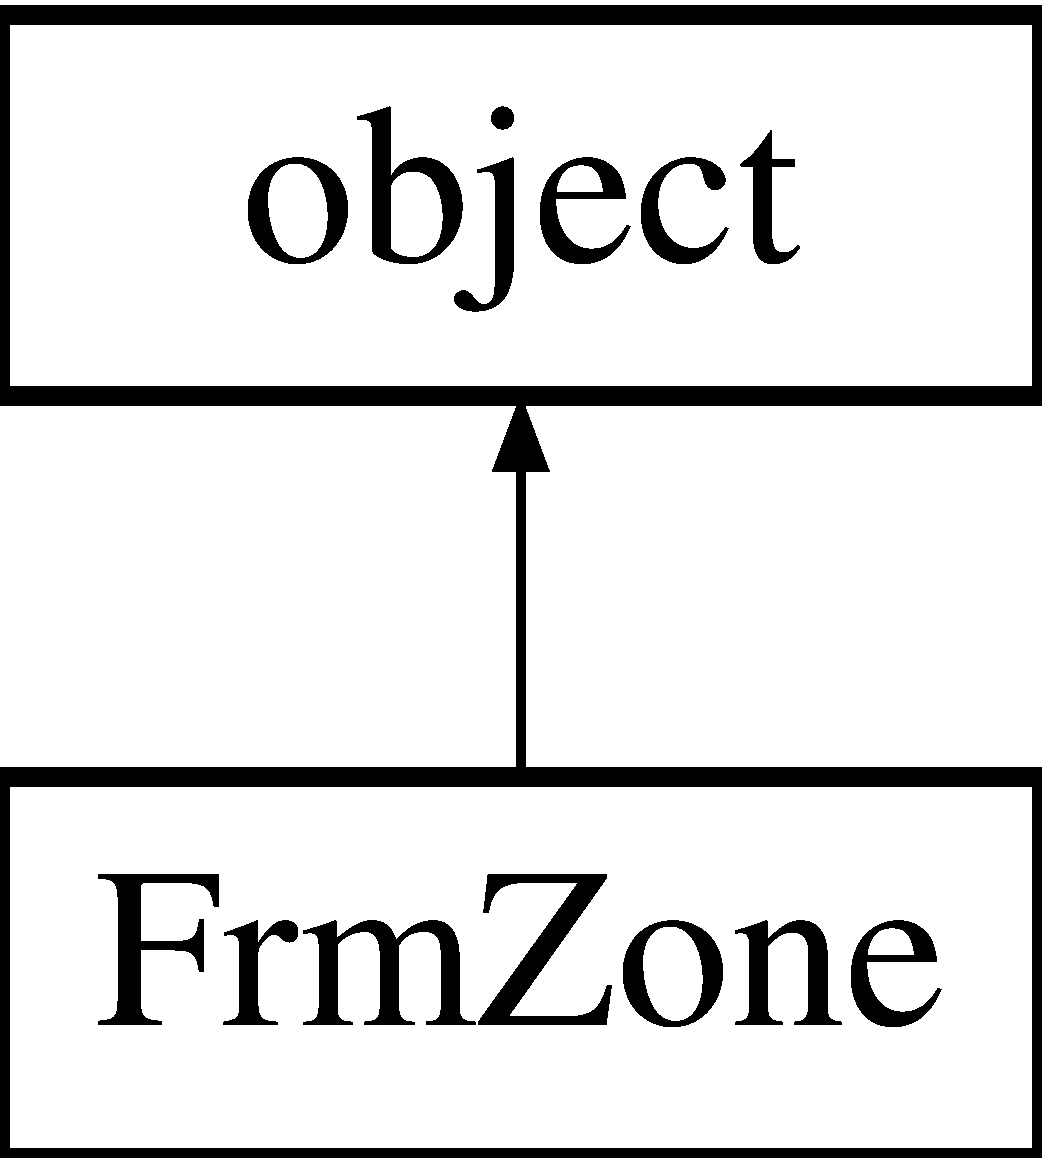
\includegraphics[height=2.000000cm]{class_f_zone_1_1_frm_zone}
\end{center}
\end{figure}
\subsection*{Public Member Functions}
\begin{DoxyCompactItemize}
\item 
\mbox{\Hypertarget{class_f_zone_1_1_frm_zone_ad5638cba1e16dbbca63151f4ac04ed4e}\label{class_f_zone_1_1_frm_zone_ad5638cba1e16dbbca63151f4ac04ed4e}} 
def {\bfseries load} (self, id=None, name=None, activities=None, ground\+Floor=None, window\+Count=None, floor\+Area=None, show=False, enabled=False)
\item 
\mbox{\Hypertarget{class_f_zone_1_1_frm_zone_ab4f4398c3f210fe4ea6e720401357691}\label{class_f_zone_1_1_frm_zone_ab4f4398c3f210fe4ea6e720401357691}} 
def {\bfseries show} (self)
\item 
\mbox{\Hypertarget{class_f_zone_1_1_frm_zone_a749ac72aadf70cac935210a79fc0cf5d}\label{class_f_zone_1_1_frm_zone_a749ac72aadf70cac935210a79fc0cf5d}} 
def {\bfseries \+\_\+\+\_\+init\+\_\+\+\_\+} (self, master, parent, id=str(uuid.\+uuid4()), name=\textquotesingle{}\textquotesingle{}, activities=\textquotesingle{}\textquotesingle{}, ground\+Floor=False, window\+Count=0, floor\+Area=0)
\end{DoxyCompactItemize}
\subsection*{Public Attributes}
\begin{DoxyCompactItemize}
\item 
\mbox{\Hypertarget{class_f_zone_1_1_frm_zone_afe9b98e5038ae1c69e5bb7eef0ed7cc4}\label{class_f_zone_1_1_frm_zone_afe9b98e5038ae1c69e5bb7eef0ed7cc4}} 
{\bfseries lblname}
\item 
\mbox{\Hypertarget{class_f_zone_1_1_frm_zone_a24025fc9f698a9db8fb4f3c1c3c32e40}\label{class_f_zone_1_1_frm_zone_a24025fc9f698a9db8fb4f3c1c3c32e40}} 
{\bfseries txtname}
\item 
\mbox{\Hypertarget{class_f_zone_1_1_frm_zone_af32c698b2c07b5cb5e325c52fe87bd31}\label{class_f_zone_1_1_frm_zone_af32c698b2c07b5cb5e325c52fe87bd31}} 
{\bfseries lblactivities}
\item 
\mbox{\Hypertarget{class_f_zone_1_1_frm_zone_a6345e3c5de5cd6dbbd7bfcfc80d84d89}\label{class_f_zone_1_1_frm_zone_a6345e3c5de5cd6dbbd7bfcfc80d84d89}} 
{\bfseries lst\+Activities}
\item 
\mbox{\Hypertarget{class_f_zone_1_1_frm_zone_a8d1352a3c37302ab5a2bb48e863aa0f4}\label{class_f_zone_1_1_frm_zone_a8d1352a3c37302ab5a2bb48e863aa0f4}} 
{\bfseries lblground\+Floor}
\item 
\mbox{\Hypertarget{class_f_zone_1_1_frm_zone_a12bdd95b96a5e4912083497d98b8bf84}\label{class_f_zone_1_1_frm_zone_a12bdd95b96a5e4912083497d98b8bf84}} 
{\bfseries chkground\+Floor}
\item 
\mbox{\Hypertarget{class_f_zone_1_1_frm_zone_a4c87625a547ea6984a6f464e6d5b04a1}\label{class_f_zone_1_1_frm_zone_a4c87625a547ea6984a6f464e6d5b04a1}} 
{\bfseries lblwindow\+Count}
\item 
\mbox{\Hypertarget{class_f_zone_1_1_frm_zone_a78810858635355bfecfd1f8230b52bbf}\label{class_f_zone_1_1_frm_zone_a78810858635355bfecfd1f8230b52bbf}} 
{\bfseries txtwindow\+Count}
\item 
\mbox{\Hypertarget{class_f_zone_1_1_frm_zone_a04b1dd26e93ab7acdaaefe7dd99bec10}\label{class_f_zone_1_1_frm_zone_a04b1dd26e93ab7acdaaefe7dd99bec10}} 
{\bfseries lblfloor\+Area}
\item 
\mbox{\Hypertarget{class_f_zone_1_1_frm_zone_a794ba46d7ec1a9ecde741e25379784f0}\label{class_f_zone_1_1_frm_zone_a794ba46d7ec1a9ecde741e25379784f0}} 
{\bfseries txtfloor\+Area}
\end{DoxyCompactItemize}


\subsection{Detailed Description}


Definition at line 14 of file F\+Zone.\+py.



The documentation for this class was generated from the following file\+:\begin{DoxyCompactItemize}
\item 
F\+Zone.\+py\end{DoxyCompactItemize}

\hypertarget{class_c_utils_1_1_utils_1_1_functions}{}\section{Utils.\+Functions Class Reference}
\label{class_c_utils_1_1_utils_1_1_functions}\index{Utils.\+Functions@{Utils.\+Functions}}
\subsection*{Static Public Member Functions}
\begin{DoxyCompactItemize}
\item 
\mbox{\Hypertarget{class_c_utils_1_1_utils_1_1_functions_a5e350b170a2f7c2a1bc0340e3d9dabe6}\label{class_c_utils_1_1_utils_1_1_functions_a5e350b170a2f7c2a1bc0340e3d9dabe6}} 
def {\bfseries concatenate\+Dict} (dictA, dictB)
\item 
\mbox{\Hypertarget{class_c_utils_1_1_utils_1_1_functions_a61ed8a6fa4067a6b22375e20bce00a1a}\label{class_c_utils_1_1_utils_1_1_functions_a61ed8a6fa4067a6b22375e20bce00a1a}} 
def {\bfseries subtract\+Dict} (dictA, dictB)
\end{DoxyCompactItemize}


\subsection{Detailed Description}


Definition at line 41 of file C\+Utils.\+py.



The documentation for this class was generated from the following file\+:\begin{DoxyCompactItemize}
\item 
C\+Utils.\+py\end{DoxyCompactItemize}

\hypertarget{class_c_simulation_1_1_simulation_1_1_no_m_a_s_s_models_1_1_heating}{}\section{Simulation.\+No\+M\+A\+S\+S\+Models.\+Heating Class Reference}
\label{class_c_simulation_1_1_simulation_1_1_no_m_a_s_s_models_1_1_heating}\index{Simulation.\+No\+M\+A\+S\+S\+Models.\+Heating@{Simulation.\+No\+M\+A\+S\+S\+Models.\+Heating}}
Inheritance diagram for Simulation.\+No\+M\+A\+S\+S\+Models.\+Heating\+:\begin{figure}[H]
\begin{center}
\leavevmode
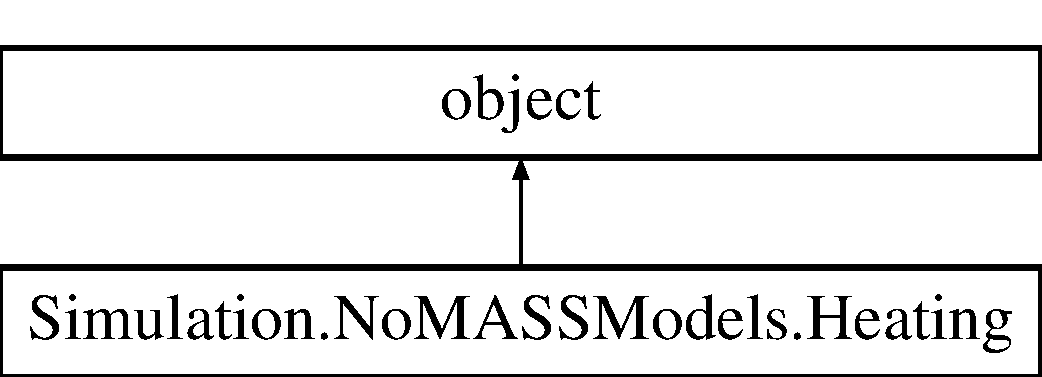
\includegraphics[height=2.000000cm]{class_c_simulation_1_1_simulation_1_1_no_m_a_s_s_models_1_1_heating}
\end{center}
\end{figure}
\subsection*{Public Member Functions}
\begin{DoxyCompactItemize}
\item 
\mbox{\Hypertarget{class_c_simulation_1_1_simulation_1_1_no_m_a_s_s_models_1_1_heating_ae64f0875afe3067b97ba370b354b9213}\label{class_c_simulation_1_1_simulation_1_1_no_m_a_s_s_models_1_1_heating_ae64f0875afe3067b97ba370b354b9213}} 
def {\bfseries \+\_\+\+\_\+init\+\_\+\+\_\+} (self)
\end{DoxyCompactItemize}
\subsection*{Public Attributes}
\begin{DoxyCompactItemize}
\item 
\mbox{\Hypertarget{class_c_simulation_1_1_simulation_1_1_no_m_a_s_s_models_1_1_heating_a91b39549c797bd5646357c8b6eecad0f}\label{class_c_simulation_1_1_simulation_1_1_no_m_a_s_s_models_1_1_heating_a91b39549c797bd5646357c8b6eecad0f}} 
{\bfseries enabled}
\end{DoxyCompactItemize}


\subsection{Detailed Description}


Definition at line 174 of file C\+Simulation.\+py.



The documentation for this class was generated from the following file\+:\begin{DoxyCompactItemize}
\item 
C\+Simulation.\+py\end{DoxyCompactItemize}

\hypertarget{class_c_utils_1_1_utils_1_1_resources_1_1_icons}{}\section{Utils.\+Resources.\+Icons Class Reference}
\label{class_c_utils_1_1_utils_1_1_resources_1_1_icons}\index{Utils.\+Resources.\+Icons@{Utils.\+Resources.\+Icons}}
\subsection*{Static Public Attributes}
\begin{DoxyCompactItemize}
\item 
\mbox{\Hypertarget{class_c_utils_1_1_utils_1_1_resources_1_1_icons_a2ebfbf8215620ef13e68eab4c6594f34}\label{class_c_utils_1_1_utils_1_1_resources_1_1_icons_a2ebfbf8215620ef13e68eab4c6594f34}} 
string {\bfseries align\+\_\+justify\+\_\+16\+\_\+0\+\_\+333333} = \char`\"{}R0l\+G\+O\+Dlh\+E\+A\+A\+Q\+A\+L\+M\+J\+A\+E\+B\+A\+Q\+F\+Z\+W\+Vl\+N\+T\+U1h\+Y\+W\+E\+F\+B\+Q\+V\+V\+V\+Vf39/fr6+j\+MzM////w\+A\+A\+A\+A\+A\+A\+A\+A\+A\+A\+A\+A\+A\+A\+A\+A\+A\+A\+A\+A\+A\+A\+A\+C\+H5\+B\+A\+E\+A\+A\+Ak\+A\+L\+A\+A\+A\+A\+A\+A\+Q\+A\+B\+A\+A\+A\+A\+Q1\+M\+Ml\+Jaz\+In670\+N\+Q\+W\+Aoik\+Qwnm\+Fgr\+V\+O\+Boo\+Xwng\+L\+L\+Dv\+M4\+A\+Lk\+I\+Y\+Jxgxg\+A\+Ucgy8\+Hghg\+Ui\+J\+Utqg0\+E\+Q\+E\+A\+Ow==\char`\"{}
\item 
\mbox{\Hypertarget{class_c_utils_1_1_utils_1_1_resources_1_1_icons_a0b147d8423a738984a4177674381f719}\label{class_c_utils_1_1_utils_1_1_resources_1_1_icons_a0b147d8423a738984a4177674381f719}} 
string {\bfseries building\+\_\+o\+\_\+16\+\_\+0\+\_\+333333} = \char`\"{}R0l\+G\+O\+Dlh\+E\+A\+A\+Q\+A\+M\+Q\+S\+A\+Pr6+l\+V\+V\+Vfj4+P\+X19\+X\+Jyckl\+J\+S\+Y\+G\+Bg\+X\+Nzc1\+N\+TU/n5+Tg4\+O\+E9\+P\+T0\+N\+D\+Q0\+F\+B\+Q\+V\+F\+R\+Ufv7+/39/T\+MzM////w\+A\+A\+A\+A\+A\+A\+A\+A\+A\+A\+A\+A\+A\+A\+A\+A\+A\+A\+A\+A\+A\+A\+A\+A\+A\+A\+A\+A\+A\+A\+A\+A\+A\+A\+A\+A\+A\+A\+A\+A\+A\+A\+A\+A\+A\+A\+A\+A\+A\+A\+A\+C\+H5\+B\+A\+E\+A\+A\+B\+I\+A\+L\+A\+A\+A\+A\+A\+A\+Q\+A\+B\+A\+A\+A\+A\+V\+Yo\+I\+R\+E\+Z\+Gk2k\+K\+R\+G\+A\+OS+7/Ko\+Ug\+Q\+F\+Em4kue\+T\+Mqx\+Rt6\+A\+P\+W\+I\+Ax\+J8i\+B\+Q\+Fmk24v\+A\+H\+F\+Uqfw\+Y\+Z\+E\+S2gmqc\+Gr\+Cnz\+Ucr3\+Yozht0z4\+A\+A\+N\+X\+X\+G\+K2\+R\+Bj\+Ryv\+Y\+Qf\+Gwsmg\+R\+E\+K\+Vmt\+S\+I\+Q\+A7\char`\"{}
\item 
\mbox{\Hypertarget{class_c_utils_1_1_utils_1_1_resources_1_1_icons_a0c38d9eab3dea717f7bef609f0f33566}\label{class_c_utils_1_1_utils_1_1_resources_1_1_icons_a0c38d9eab3dea717f7bef609f0f33566}} 
string {\bfseries cube\+\_\+16\+\_\+0\+\_\+333333} = \char`\"{}R0l\+G\+O\+Dlh\+E\+A\+A\+Q\+A\+N\+U6\+A\+Pr6+jg4\+O\+Ex\+M\+T\+I\+G\+Bg\+T\+Y2\+Njk5\+Off399\+T\+U1\+N\+L\+S0oi\+Ii\+M\+T\+Ex\+I2\+Njaysr\+G\+Fh\+Y\+W\+Nj\+Y3t7e/Hx8b\+Gxs\+X\+V1d\+V\+Z\+W\+Vsb\+Gxm5ubvv7+/X19e\+Li4t\+P\+T09\+D\+Q0L+/v+np6\+U\+F\+B\+Qd\+X\+V1fj4+O\+Tk5\+H\+Z2dsn\+Jyc\+X\+Fx\+X\+Jycn\+Fxcbu7u5\+S\+Ul\+E1\+N\+Tdn\+Z2d3d3\+U\+B\+A\+Q\+D\+U1\+N\+Xd3d5e\+Xl+7u7s\+P\+Dw4m\+Jie\+Xl5fb29kd\+H\+R1\+V\+V\+Vfn5+f39/cz\+Mz\+D\+Mz\+M////w\+A\+A\+A\+A\+A\+A\+A\+A\+A\+A\+A\+A\+A\+A\+A\+A\+A\+A\+A\+C\+H5\+B\+A\+E\+A\+A\+Do\+A\+L\+A\+A\+A\+A\+A\+A\+Q\+A\+B\+A\+A\+A\+Aa\+B\+Q\+J1\+Qa\+F\+M0\+Gi\+Pbc\+Hn\+L\+S\+A\+In\+U\+Gq\+Q\+Cx1u\+Qsi\+C0\+P\+Jghx\+Y\+Nib\+C\+A\+C\+B6fp\+Vpn\+G\+Ahyucn\+Gs\+L6\+Yag\+W4\+Pld\+C3\+Gw\+U\+Dg\+Uu\+Mj\+N7hyw\+J\+Kl8\+Ah3siao2\+Oc\+Di\+Rk5\+S\+Wl5\+V\+L\+Njkxk5t\+C\+G\+A4\+J\+Ogcoh5sc\+F\+Q\+I\+I\+Swodejgv\+Dyswazo3\+E\+Q\+E5\+N\+A\+E\+R\+X7g6\+Ngw\+M\+Smp\+B\+A\+Ds=\char`\"{}
\item 
\mbox{\Hypertarget{class_c_utils_1_1_utils_1_1_resources_1_1_icons_ae511484adf0a80407269ea076410dced}\label{class_c_utils_1_1_utils_1_1_resources_1_1_icons_ae511484adf0a80407269ea076410dced}} 
string {\bfseries file\+\_\+o\+\_\+16\+\_\+0\+\_\+333333} = \char`\"{}R0l\+G\+O\+Dlh\+E\+A\+A\+Q\+A\+L\+M\+N\+A\+Pr6+k\+N\+D\+Q2lpacj\+Iy\+J6enrm5uba2tnl5e\+U1\+N\+Tcz\+MzJ+fn/39/T\+MzM////w\+A\+A\+A\+A\+A\+A\+A\+C\+H5\+B\+A\+E\+A\+A\+A0\+A\+L\+A\+A\+A\+A\+A\+A\+Q\+A\+B\+A\+A\+A\+A\+R\+Es\+B1\+G\+Kwul6c3A+h/A\+D\+Mqm\+M\+Yv\+Z\+L\+Ey\+T\+E\+Caqstpgc\+Km\+K\+V\+A\+Guaq\+H\+W\+Kfdb\+C\+Ruyot\+Gnp\+A2\+Vy2fzm\+Cw6kc\+Tftao9\+Cixgig\+A\+Kj\+Q\+A\+A\+Ow==\char`\"{}
\item 
\mbox{\Hypertarget{class_c_utils_1_1_utils_1_1_resources_1_1_icons_a96f7dd9314915fac14d358de623dfbbc}\label{class_c_utils_1_1_utils_1_1_resources_1_1_icons_a96f7dd9314915fac14d358de623dfbbc}} 
string {\bfseries folder\+\_\+16\+\_\+0\+\_\+d4be2b} = \char`\"{}R0l\+G\+O\+Dlh\+E\+A\+A\+Q\+A\+I\+Q\+W\+A\+NS+K9S+K9S+K9S+K9S+K9S+K9S+K9S+K9S+K9S+K9S+K9S+K9S+K9S+K9S+K9S+K9S+K9S+K9S+K9S+K9S+K9S+K////////////////////////////////////////y\+H5\+B\+A\+E\+K\+A\+B8\+A\+L\+A\+A\+A\+A\+A\+A\+Q\+A\+B\+A\+A\+Q\+A\+U04\+Ce\+O\+Z\+Pl\+Va\+Kquz4p\+O\+Uhx\+Homujzqky5njbjZ/r8\+Y\+E\+I\+Kx\+Reb/m\+Zu\+Jh\+Hl\+S5aa\+V\+Gr16q\+Ryly\+G\+A\+A\+A7\char`\"{}
\item 
\mbox{\Hypertarget{class_c_utils_1_1_utils_1_1_resources_1_1_icons_a09d233da2d08db5e58ece97e1f653242}\label{class_c_utils_1_1_utils_1_1_resources_1_1_icons_a09d233da2d08db5e58ece97e1f653242}} 
string {\bfseries folder\+\_\+o\+\_\+16\+\_\+0\+\_\+d4be2b} = \char`\"{}R0l\+G\+O\+Dlh\+E\+A\+A\+Q\+A\+I\+Q\+Y\+A\+NS+K9S+K9S+K9S+K9S+K9S+K9S+K9S+K9S+K9S+K9S+K9S+K9S+K9S+K9S+K9S+K9S+K9S+K9S+K9S+K9S+K9S+K9S+K9S+K////////////////////////////////y\+H5\+B\+A\+E\+K\+A\+B8\+A\+L\+A\+A\+A\+A\+A\+A\+Q\+A\+B\+A\+A\+Q\+A\+Uy4\+Ce\+O\+Z\+Pld\+Znqi\+J\+H\+W9s\+N\+Wcqol\+Wc\+U3r48v3nwhs\+S\+I\+T8\+Sp\+M\+S\+K7\+Xk\+O\+Zo631\+H6u0i\+Onwd\+W\+F\+A\+I\+A\+Ow==\char`\"{}
\item 
\mbox{\Hypertarget{class_c_utils_1_1_utils_1_1_resources_1_1_icons_a13a639e8075d476a6a40b77cdfd253b7}\label{class_c_utils_1_1_utils_1_1_resources_1_1_icons_a13a639e8075d476a6a40b77cdfd253b7}} 
string {\bfseries folder\+\_\+open\+\_\+16\+\_\+0\+\_\+d4be2b} = \char`\"{}R0l\+G\+O\+Dlh\+E\+A\+A\+Q\+A\+K\+Ul\+A\+NS+K9S+K9S+K9S+K9S+K9S+K9S+K9S+K9S+K9S+K9S+K9S+K9S+K9S+K9S+K9S+K9S+K9S+K9S+K9S+K9S+K9S+K9S+K9S+K9S+K9S+K9S+K9S+K9S+K9S+K9S+K9S+K9S+K9S+K9S+K9S+K9S+K////////////////////////////////////////////////////////////////////////////////////////////////////////////y\+H5\+B\+A\+E\+K\+A\+D8\+A\+L\+A\+A\+A\+A\+A\+A\+Q\+A\+B\+A\+A\+A\+A\+Y9w\+J9w\+S\+Cwaj8\+U\+Ra\+Xl\+B\+Cj/Lq\+P\+M\+Xr\+V\+Y3\+R\+Ku\+W\+Z\+Blur\+Rrv\+Ej\+Q\+V\+Lj1ls0jI+S6pwo6b\+R\+Bli5pms\+Gz0\+Uf\+U\+M\+Va\+Y\+Jl\+Q\+Q\+A7\char`\"{}
\item 
\mbox{\Hypertarget{class_c_utils_1_1_utils_1_1_resources_1_1_icons_a943d560bd69b38e2a6f17ab78e0496af}\label{class_c_utils_1_1_utils_1_1_resources_1_1_icons_a943d560bd69b38e2a6f17ab78e0496af}} 
string {\bfseries folder\+\_\+open\+\_\+o\+\_\+16\+\_\+0\+\_\+d4be2b} = \char`\"{}R0l\+G\+O\+Dlh\+E\+A\+A\+Q\+A\+K\+Um\+A\+NS+K9S+K9S+K9S+K9S+K9S+K9S+K9S+K9S+K9S+K9S+K9S+K9S+K9S+K9S+K9S+K9S+K9S+K9S+K9S+K9S+K9S+K9S+K9S+K9S+K9S+K9S+K9S+K9S+K9S+K9S+K9S+K9S+K9S+K9S+K9S+K9S+K9S+K////////////////////////////////////////////////////////////////////////////////////////////////////////y\+H5\+B\+A\+E\+K\+A\+D8\+A\+L\+A\+A\+A\+A\+A\+A\+Q\+A\+B\+A\+A\+Q\+AY/w\+J9w\+S\+Cz+Sk\+N\+Maclkko5\+E\+Zf\+N\+C1\+Bi\+L\+F\+C\+K\+Iwwldicivc\+D\+R\+Eds\+T\+C\+D\+HrN/h\+B\+F6\+L\+C4\+Ul7\+Lw5y1pu\+R\+Z\+W4\+Yb\+T\+Y\+J5b\+Fd\+B\+A\+Ds=\char`\"{}
\item 
\mbox{\Hypertarget{class_c_utils_1_1_utils_1_1_resources_1_1_icons_a37411c4297633ea55fab72a54cd75cfb}\label{class_c_utils_1_1_utils_1_1_resources_1_1_icons_a37411c4297633ea55fab72a54cd75cfb}} 
string {\bfseries folder\+\_\+open\+\_\+o\+\_\+16\+\_\+0\+\_\+333333} = \char`\"{}R0l\+G\+O\+Dlh\+E\+A\+A\+Q\+A\+N\+Uj\+A\+F\+F\+R\+Ufv7+2\+Vl\+Z\+V\+V\+V\+Venp6d\+L\+S0u3t7fb29ujo6\+Hp6eqysr\+P\+Dw8\+H\+Z2durq6kl\+J\+S\+V\+Z\+W\+Vmlpaefn57\+S0t\+Dg4\+O\+Ex\+M\+T\+D09\+Pa2tr\+U\+B\+A\+Q\+Mb\+Gxj\+U1\+Nc\+L\+Cwk9\+P\+T+7u7vz8/\+Pj4+\+P\+Ly8j\+Y2\+Nv39/\+T\+Mz\+M////w\+A\+A\+A\+A\+A\+A\+A\+A\+A\+A\+A\+A\+A\+A\+A\+A\+A\+A\+A\+A\+A\+A\+A\+A\+A\+A\+A\+A\+A\+A\+A\+A\+A\+A\+A\+A\+A\+A\+A\+A\+A\+A\+A\+A\+A\+A\+A\+A\+A\+A\+A\+A\+A\+A\+A\+A\+A\+A\+A\+A\+A\+A\+A\+A\+A\+A\+A\+A\+A\+A\+A\+A\+A\+A\+A\+A\+A\+A\+A\+A\+A\+A\+A\+A\+A\+A\+A\+A\+A\+A\+A\+A\+A\+A\+A\+A\+A\+A\+A\+A\+A\+A\+A\+A\+A\+A\+A\+A\+A\+A\+A\+C\+H5\+B\+A\+E\+A\+A\+C\+M\+A\+L\+A\+A\+A\+A\+A\+A\+Q\+A\+B\+A\+A\+A\+A\+Zew\+J\+Fw\+S\+Cw\+K\+Q4\+F\+Ay\+Fgs\+X\+A\+C\+Aio\+Y5d\+Hi\+En\+Ql\+V\+K\+Fo\+K\+Ba\+Jw\+W\+H\+A\+Ydrc\+Rhtn\+L\+D\+I\+H\+W24\+A\+I3g\+C\+L76\+K\+Moms\+A\+G\+L\+Y\+L\+Ay\+Ic\+Gx9x\+Dw\+Qi\+F\+Ahb\+I\+R\+A\+F\+Iw\+M\+W\+I\+Z\+S\+Vl\+Qc\+J\+Ek\+I\+E\+A\+Hh3\+A\+Bhboq\+N\+F\+Q\+Q\+A7\char`\"{}
\item 
\mbox{\Hypertarget{class_c_utils_1_1_utils_1_1_resources_1_1_icons_a0388770817b17ab7e96a521756146b17}\label{class_c_utils_1_1_utils_1_1_resources_1_1_icons_a0388770817b17ab7e96a521756146b17}} 
string {\bfseries folder\+\_\+open\+\_\+o\+\_\+16\+\_\+0\+\_\+bfa600} = \char`\"{}R0l\+G\+O\+Dlh\+E\+A\+A\+Q\+A\+K\+Um\+AL+m\+AL+m\+AL+m\+AL+m\+AL+m\+AL+m\+AL+m\+AL+m\+AL+m\+AL+m\+AL+m\+AL+m\+AL+m\+AL+m\+AL+m\+AL+m\+AL+m\+AL+m\+AL+m\+AL+m\+AL+m\+AL+m\+AL+m\+AL+m\+AL+m\+AL+m\+AL+m\+AL+m\+AL+m\+AL+m\+AL+m\+AL+m\+AL+m\+AL+m\+AL+m\+AL+m\+AL+m\+AL+m\+AP///////////////////////////////////////////////////////////////////////////////////////////////////////y\+H5\+B\+A\+E\+K\+A\+D8\+A\+L\+A\+A\+A\+A\+A\+A\+Q\+A\+B\+A\+A\+A\+AY/w\+J9w\+S\+Cwaj0\+U\+Qhx\+N\+C\+Dj9\+Ekf\+N\+X\+Im\+J\+K\+W\+Oy\+F\+W\+J1\+Whl3n\+C\+Dylko\+X\+Xr\+Lp\+E\+Mv84\+Z\+U21\+U85\+Q\+P\+W\+W\+L\+U\+F\+Om\+E\+Ddran\+Blh\+I\+R\+B\+A\+Ds=\char`\"{}
\item 
\mbox{\Hypertarget{class_c_utils_1_1_utils_1_1_resources_1_1_icons_a71773fac9f40ecfa566df34ef1d9bb85}\label{class_c_utils_1_1_utils_1_1_resources_1_1_icons_a71773fac9f40ecfa566df34ef1d9bb85}} 
string {\bfseries info\+\_\+circle\+\_\+16\+\_\+0\+\_\+00aa00} = \char`\"{}R0l\+G\+O\+Dlh\+E\+A\+A\+Q\+A\+K\+Uy\+A\+A\+Cq\+A\+A\+Cq\+A\+A\+Cq\+A\+A\+Cq\+A\+A\+Cq\+A\+A\+Cq\+A\+A\+Cq\+A\+A\+Cq\+A\+A\+Cq\+A\+A\+Cq\+A\+A\+Cq\+A\+A\+Cq\+A\+A\+Cq\+A\+A\+Cq\+A\+A\+Cq\+A\+A\+Cq\+A\+A\+Cq\+A\+A\+Cq\+A\+A\+Cq\+A\+A\+Cq\+A\+A\+Cq\+A\+A\+Cq\+A\+A\+Cq\+A\+A\+Cq\+A\+A\+Cq\+A\+A\+Cq\+A\+A\+Cq\+A\+A\+Cq\+A\+A\+Cq\+A\+A\+Cq\+A\+A\+Cq\+A\+A\+Cq\+A\+A\+Cq\+A\+A\+Cq\+A\+A\+Cq\+A\+A\+Cq\+A\+A\+Cq\+A\+A\+Cq\+A\+A\+Cq\+A\+A\+Cq\+A\+A\+Cq\+A\+A\+Cq\+A\+A\+Cq\+A\+A\+Cq\+A\+A\+Cq\+A\+A\+Cq\+A\+A\+Cq\+A\+A\+Cq\+A\+A\+Cq\+A\+A\+Cq\+AP///////////////////////////////////////////////////////y\+H5\+B\+A\+E\+K\+A\+D8\+A\+L\+A\+A\+A\+A\+A\+A\+Q\+A\+B\+A\+A\+Q\+A\+Z\+Sw\+J9w\+O\+H\+Kd\+Ps\+Ph\+Ks\+Zk\+Dpt\+N\+I\+X\+Q\+K\+R\+Qp\+Nzm\+Qq\+Oyx\+Fpd+f\+Cpqkgrl\+C\+U\+R\+O\+U\+H\+J\+Jc\+K\+Gtb2\+G\+G\+Gw\+Ky2h3y\+Ov\+Y\+Qbf\+H1\+O\+M\+F\+N\+Pho\+G\+C\+Zj8g\+Y\+U\+Ic\+T\+H9\+Jd\+V\+Qtc5e\+X\+Q\+Q\+A7\char`\"{}
\item 
\mbox{\Hypertarget{class_c_utils_1_1_utils_1_1_resources_1_1_icons_a5c77f6999994712634e7074df69da2c6}\label{class_c_utils_1_1_utils_1_1_resources_1_1_icons_a5c77f6999994712634e7074df69da2c6}} 
string {\bfseries save\+\_\+16\+\_\+0\+\_\+333333} = \char`\"{}R0l\+G\+O\+Dlh\+E\+A\+A\+Q\+A\+M\+Qa\+A\+Nj\+Y2\+E\+F\+B\+Qf\+X19fz8/G9vb0\+N\+D\+Q8\+H\+Bw\+W\+Bg\+Y\+J\+G\+Rkb\+Gxsd\+D\+Q0\+Fxc\+X\+Gpqas\+T\+Ex\+G\+Fh\+Y\+W\+Vl\+Zfn5+e\+Xl5\+Tg4\+O\+L\+Cws\+Glpaa\+Cgo\+G1tbf39/fr6+j\+MzM////w\+A\+A\+A\+A\+A\+A\+A\+A\+A\+A\+A\+A\+A\+A\+A\+A\+A\+A\+A\+C\+H5\+B\+A\+E\+A\+A\+Bo\+A\+L\+A\+A\+A\+A\+A\+A\+Q\+A\+B\+A\+A\+A\+A\+Vg\+I\+J\+O\+N\+J\+Bk0\+Wqpl\+Ak\+Vec\+B\+Y9k5ph\+Fmljg5\+Okt9xopxkc\+D\+Cuc\+Doh\+J\+Q\+S\+R\+J\+R\+Gl\+Uu\+Oxu\+Gox2q2\+Jiu2\+Bv\+Uw\+Mrw66\+Yyr\+R\+E\+S\+A\+Y\+V5r\+Ig48\+Y\+Bwln6\+L\+Xg\+PY/R/dnh/S\+Qtrhw\+F\+W\+W4u\+M\+G\+F\+Yh\+A\+Ds=\char`\"{}
\item 
\mbox{\Hypertarget{class_c_utils_1_1_utils_1_1_resources_1_1_icons_ac6e4184b2e2aa368675e72b8d515c1a8}\label{class_c_utils_1_1_utils_1_1_resources_1_1_icons_ac6e4184b2e2aa368675e72b8d515c1a8}} 
string {\bfseries th\+\_\+large\+\_\+16\+\_\+0\+\_\+333333} = \char`\"{}R0l\+G\+O\+Dlh\+E\+A\+A\+Q\+A\+L\+M\+M\+A\+K\+Wlpf\+Dw8\+F\+N\+T\+U2dn\+Z2lpa\+Z\+G\+Rk\+Z\+S\+Ul\+F\+V\+V\+V\+T\+U1\+Ne/v7/39/T\+MzM////w\+A\+A\+A\+A\+A\+A\+A\+A\+A\+A\+A\+C\+H5\+B\+A\+E\+A\+A\+Aw\+A\+L\+A\+A\+A\+A\+A\+A\+Q\+A\+B\+A\+A\+A\+A\+R\+Ek\+Ml\+J61\+R\+Y0ax\+Z\+W\+S\+Ao\+Y\+E\+I\+Ifia\+Y\+J\+Gkbrq4\+Lt0gb\+B\+D\+R\+Qhw\+N\+Gm\+Ai\+Ah\+L\+P\+J\+S\+AypA+a\+Q\+Qr\+Zm\+M\+R\+M0qm\+L\+Rb\+Lh\+Uc\+Afq\+K\+X6ho\+G\+U8i\+Q\+A\+A\+Ow==\char`\"{}
\item 
\mbox{\Hypertarget{class_c_utils_1_1_utils_1_1_resources_1_1_icons_ada89a45b7e7c43a26fa9d49cc22f3590}\label{class_c_utils_1_1_utils_1_1_resources_1_1_icons_ada89a45b7e7c43a26fa9d49cc22f3590}} 
string {\bfseries user\+\_\+o\+\_\+16\+\_\+0\+\_\+333333} = \char`\"{}R0l\+G\+O\+Dlh\+E\+A\+A\+Q\+A\+N\+Ur\+A\+P\+Dw8\+Pz8/Glpaf39/e/v7zg4\+O\+M\+H\+Bw\+Ts7\+O2dn\+Z0\+V\+F\+Rc7\+Ozs3\+Nz\+Tk5\+O\+T4+Pm\+Bg\+Y\+P\+Pz84\+S\+Eh\+Ed\+H\+R4a\+Ghu\+Li4tra2qioq\+Li4u\+Jm\+Zm\+Ze\+Xl8j\+Iy\+K2tr\+U9\+PT/X19\+U\+B\+A\+Q\+O3t7\+Wpqap\+W\+Vl\+Yi\+Ii\+Pn5+db\+W1sn\+Jyb\+Gxs\+T09\+P\+Y\+W\+Fh\+V\+F\+R\+U\+Y\+O\+Dgz\+MzM////w\+A\+A\+A\+A\+A\+A\+A\+A\+A\+A\+A\+A\+A\+A\+A\+A\+A\+A\+A\+A\+A\+A\+A\+A\+A\+A\+A\+A\+A\+A\+A\+A\+A\+A\+A\+A\+A\+A\+A\+A\+A\+A\+A\+A\+A\+A\+A\+A\+A\+A\+A\+A\+A\+A\+A\+A\+A\+A\+A\+A\+A\+A\+A\+A\+A\+A\+A\+A\+A\+A\+A\+A\+A\+A\+A\+A\+A\+A\+A\+C\+H5\+B\+A\+E\+A\+A\+Cs\+A\+L\+A\+A\+A\+A\+A\+A\+Q\+A\+B\+A\+A\+A\+A\+Zxw\+J\+V\+Qu\+E\+C\+Y\+B\+Iqhcnh\+K\+E\+Q\+K\+E\+V\+Gg5\+X\+K\+S\+Wq\+S\+R\+V\+A\+Fg\+S\+Pt\+R\+V\+I7\+A\+M\+N\+M\+K\+Irp\+Ig\+C\+Gcg\+W\+B\+J1\+Eil\+A\+A\+A\+F\+Aqp\+Cg\+K\+Dk\+R\+X\+Q\+Y\+O\+D\+A4\+G\+Kw8b\+Hk\+M\+Vh2\+Er\+Ix\+J\+D\+Ag+P\+Kw\+M\+H\+Qwlklg\+U\+D\+Qigilis\+M\+Qx\+Y\+Yn2\+El\+I\+Eoa\+H\+Sqws\+So\+H\+F6mj\+V\+E\+E\+A\+Ow==\char`\"{}
\item 
\mbox{\Hypertarget{class_c_utils_1_1_utils_1_1_resources_1_1_icons_af47ddce59f48636391343fb129f34833}\label{class_c_utils_1_1_utils_1_1_resources_1_1_icons_af47ddce59f48636391343fb129f34833}} 
string {\bfseries chevron\+\_\+circle\+\_\+up\+\_\+16\+\_\+0\+\_\+333333} = \char`\"{}R0l\+G\+O\+Dlh\+E\+A\+A\+Q\+A\+K\+U8\+A\+D\+Mz\+Mz\+Mz\+Mz\+Mz\+Mz\+Mz\+Mz\+Mz\+Mz\+Mz\+Mz\+Mz\+Mz\+Mz\+Mz\+Mz\+Mz\+Mz\+Mz\+Mz\+Mz\+Mz\+Mz\+Mz\+Mz\+Mz\+Mz\+Mz\+Mz\+Mz\+Mz\+Mz\+Mz\+Mz\+Mz\+Mz\+Mz\+Mz\+Mz\+Mz\+Mz\+Mz\+Mz\+Mz\+Mz\+Mz\+Mz\+Mz\+Mz\+Mz\+Mz\+Mz\+Mz\+Mz\+Mz\+Mz\+Mz\+Mz\+Mz\+Mz\+Mz\+Mz\+Mz\+Mz\+Mz\+Mz\+Mz\+Mz\+Mz\+Mz\+Mz\+Mz\+Mz\+Mz\+Mz\+Mz\+Mz\+Mz\+Mz\+Mz\+Mz\+Mz\+Mz\+Mz\+Mz\+Mz\+Mz\+Mz\+Mz\+Mz\+Mz\+Mz\+Mz\+Mz\+Mz\+Mz\+Mz\+Mz\+Mz\+Mz\+Mz\+Mz\+Mz\+Mz\+Mz\+Mz\+Mz\+Mz\+Mz\+Mz\+Mz\+Mz\+Mz\+Mz\+Mz\+Mz\+Mz\+MzM////////////////y\+H5\+B\+A\+E\+K\+A\+D8\+A\+L\+A\+A\+A\+A\+A\+A\+Q\+A\+B\+A\+A\+A\+A\+Zfw\+J9\+Qq\+Mrtdr\+Ghknhs\+Hm/L\+H8x\+J3\+Sl\+T\+Tij\+Kq\+Rtmhybn6idq\+Qp\+Ul5+91t\+E\+V/p\+O\+Y\+Pt6uhla\+Pj\+T2\+Ydnn\+Y4\+Snpx\+M0\+Jb\+R4\+F\+Cej9\+P\+U1wu\+Ry1\+C\+L\+F\+V\+V\+Sj\+S\+Vckstm\+W9\+C\+M\+U06\+J56k\+Sk\+E\+A\+Ow==\char`\"{}
\item 
\mbox{\Hypertarget{class_c_utils_1_1_utils_1_1_resources_1_1_icons_ac18ab620cef96bc7d80109807dc0083a}\label{class_c_utils_1_1_utils_1_1_resources_1_1_icons_ac18ab620cef96bc7d80109807dc0083a}} 
string {\bfseries chevron\+\_\+circle\+\_\+down\+\_\+16\+\_\+0\+\_\+333333} = \char`\"{}R0l\+G\+O\+Dlh\+E\+A\+A\+Q\+A\+K\+U6\+A\+D\+Mz\+Mz\+Mz\+Mz\+Mz\+Mz\+Mz\+Mz\+Mz\+Mz\+Mz\+Mz\+Mz\+Mz\+Mz\+Mz\+Mz\+Mz\+Mz\+Mz\+Mz\+Mz\+Mz\+Mz\+Mz\+Mz\+Mz\+Mz\+Mz\+Mz\+Mz\+Mz\+Mz\+Mz\+Mz\+Mz\+Mz\+Mz\+Mz\+Mz\+Mz\+Mz\+Mz\+Mz\+Mz\+Mz\+Mz\+Mz\+Mz\+Mz\+Mz\+Mz\+Mz\+Mz\+Mz\+Mz\+Mz\+Mz\+Mz\+Mz\+Mz\+Mz\+Mz\+Mz\+Mz\+Mz\+Mz\+Mz\+Mz\+Mz\+Mz\+Mz\+Mz\+Mz\+Mz\+Mz\+Mz\+Mz\+Mz\+Mz\+Mz\+Mz\+Mz\+Mz\+Mz\+Mz\+Mz\+Mz\+Mz\+Mz\+Mz\+Mz\+Mz\+Mz\+Mz\+Mz\+Mz\+Mz\+Mz\+Mz\+Mz\+Mz\+Mz\+Mz\+Mz\+Mz\+Mz\+Mz\+Mz\+Mz\+Mz\+Mz\+Mz\+Mz\+MzM////////////////////////y\+H5\+B\+A\+E\+K\+A\+D8\+A\+L\+A\+A\+A\+A\+A\+A\+Q\+A\+B\+A\+A\+A\+A\+Zaw\+J9\+Qi\+Lrlcr\+Chknhs\+Hmv\+L38t\+Jz\+Sl\+N\+V\+Spu2\+D\+R\+Svanf\+K\+Hc\+Tspz\+C0/Hnsg5\+Xa67\+Vlosp\+Vct17\+GiP/po/J\+E0y\+U\+Wh/T\+T\+N\+K\+Ti1m\+Tom\+Hg\+E\+M0\+W\+Z\+F\+K\+L\+ZR+Qj\+B\+N\+O\+C\+W\+Zn0p\+B\+A\+Ds=\char`\"{}
\item 
\mbox{\Hypertarget{class_c_utils_1_1_utils_1_1_resources_1_1_icons_a31e01a88bed641ac821b24ec3a4b16a0}\label{class_c_utils_1_1_utils_1_1_resources_1_1_icons_a31e01a88bed641ac821b24ec3a4b16a0}} 
string {\bfseries angle\+\_\+double\+\_\+up\+\_\+16\+\_\+0\+\_\+333333} = \char`\"{}R0l\+G\+O\+Dlh\+E\+A\+A\+Q\+A\+K\+Uq\+A\+D\+Mz\+Mz\+Mz\+Mz\+Mz\+Mz\+Mz\+Mz\+Mz\+Mz\+Mz\+Mz\+Mz\+Mz\+Mz\+Mz\+Mz\+Mz\+Mz\+Mz\+Mz\+Mz\+Mz\+Mz\+Mz\+Mz\+Mz\+Mz\+Mz\+Mz\+Mz\+Mz\+Mz\+Mz\+Mz\+Mz\+Mz\+Mz\+Mz\+Mz\+Mz\+Mz\+Mz\+Mz\+Mz\+Mz\+Mz\+Mz\+Mz\+Mz\+Mz\+Mz\+Mz\+Mz\+Mz\+Mz\+Mz\+Mz\+Mz\+Mz\+Mz\+Mz\+Mz\+Mz\+Mz\+Mz\+Mz\+Mz\+Mz\+Mz\+Mz\+Mz\+Mz\+Mz\+Mz\+Mz\+Mz\+Mz\+Mz\+Mz\+Mz\+Mz\+MzM////////////////////////////////////////////////////////////////////////////////////////y\+H5\+B\+A\+E\+K\+A\+D8\+A\+L\+A\+A\+A\+A\+A\+A\+Q\+A\+B\+A\+A\+Q\+A\+Zcw\+J9w\+S\+Cw\+K\+P8\+N\+S\+Cp\+U6\+D\+Tv\+F\+Sio05\+K\+Qyx\+V\+Eq\+Yvw5\+Uqau\+J\+U\+X\+G\+Gikp0\+F\+Dy\+T\+G\+G\+Kp\+N\+Rk+A137/jf\+W\+JP/Sal\+W\+Zk\+Voak\+Qdbk\+M\+Pa\+Ul\+N\+Qx4p\+F3\+By\+Xo1\+Gc\+Wx\+Ed\+U\+Mb\+K\+R\+B4\+Xy\+J9\+Rk\+E\+A\+Ow==\char`\"{}
\item 
\mbox{\Hypertarget{class_c_utils_1_1_utils_1_1_resources_1_1_icons_a2d168ca7b55270d71ef0f1d45263e5ff}\label{class_c_utils_1_1_utils_1_1_resources_1_1_icons_a2d168ca7b55270d71ef0f1d45263e5ff}} 
string {\bfseries angle\+\_\+double\+\_\+down\+\_\+16\+\_\+0\+\_\+333333} = \char`\"{}R0l\+G\+O\+Dlh\+E\+A\+A\+Q\+A\+K\+Un\+A\+D\+Mz\+Mz\+Mz\+Mz\+Mz\+Mz\+Mz\+Mz\+Mz\+Mz\+Mz\+Mz\+Mz\+Mz\+Mz\+Mz\+Mz\+Mz\+Mz\+Mz\+Mz\+Mz\+Mz\+Mz\+Mz\+Mz\+Mz\+Mz\+Mz\+Mz\+Mz\+Mz\+Mz\+Mz\+Mz\+Mz\+Mz\+Mz\+Mz\+Mz\+Mz\+Mz\+Mz\+Mz\+Mz\+Mz\+Mz\+Mz\+Mz\+Mz\+Mz\+Mz\+Mz\+Mz\+Mz\+Mz\+Mz\+Mz\+Mz\+Mz\+Mz\+Mz\+Mz\+Mz\+Mz\+Mz\+Mz\+Mz\+Mz\+Mz\+Mz\+Mz\+Mz\+Mz\+Mz\+Mz\+MzM////////////////////////////////////////////////////////////////////////////////////////////////////y\+H5\+B\+A\+E\+K\+A\+D8\+A\+L\+A\+A\+A\+A\+A\+A\+Q\+A\+B\+A\+A\+Q\+A\+Z\+Nw\+J9w\+S\+Cw\+K\+Ta\+Rhxs\+Q\+Zjkz\+Epaj4\+Y\+Rq\+Ppd/Ti\+D\+G\+Frk\+K\+Qa\+V\+OU/jz\+W\+K7\+K4\+BR/dX/c\+Pp\+P\+Req82oa\+Sr\+E\+Ez\+V\+J\+Qksma\+Vod\+Q2t\+Gb\+U\+W\+J\+Wl\+Byh\+I9yk0\+E\+A\+Ow==\char`\"{}
\item 
\mbox{\Hypertarget{class_c_utils_1_1_utils_1_1_resources_1_1_icons_a544a4512bb037c433071a6012e9ffe28}\label{class_c_utils_1_1_utils_1_1_resources_1_1_icons_a544a4512bb037c433071a6012e9ffe28}} 
string {\bfseries angle\+\_\+up\+\_\+16\+\_\+0\+\_\+333333} = \char`\"{}R0l\+G\+O\+Dlh\+E\+A\+A\+Q\+A\+I\+Q\+W\+A\+D\+Mz\+Mz\+Mz\+Mz\+Mz\+Mz\+Mz\+Mz\+Mz\+Mz\+Mz\+Mz\+Mz\+Mz\+Mz\+Mz\+Mz\+Mz\+Mz\+Mz\+Mz\+Mz\+Mz\+Mz\+Mz\+Mz\+Mz\+Mz\+Mz\+Mz\+Mz\+Mz\+Mz\+Mz\+Mz\+Mz\+Mz\+Mz\+Mz\+Mz\+Mz\+Mz\+MzM////////////////////////////////////////y\+H5\+B\+A\+E\+K\+A\+B8\+A\+L\+A\+A\+A\+A\+A\+A\+Q\+A\+B\+A\+A\+Q\+A\+Uy4\+Ce\+O\+Z\+Dl\+Gl\+V\+Mu1\+W\+Se7\+Sv\+P9\+Iw+nx\+K\+T\+U\+N\+X\+Mj\+Iqk\+Riwa\+S\+Sj\+K7o\+V\+Si\+Vgu\+Z\+Oo\+F\+H\+S\+Vqi\+K\+N2\+F\+A\+I\+A\+Ow==\char`\"{}
\item 
\mbox{\Hypertarget{class_c_utils_1_1_utils_1_1_resources_1_1_icons_a978c4593cf1b4977e728f768bfef80ed}\label{class_c_utils_1_1_utils_1_1_resources_1_1_icons_a978c4593cf1b4977e728f768bfef80ed}} 
string {\bfseries angle\+\_\+down\+\_\+16\+\_\+0\+\_\+333333} = \char`\"{}R0l\+G\+O\+Dlh\+E\+A\+A\+Q\+A\+I\+Q\+S\+A\+D\+Mz\+Mz\+Mz\+Mz\+Mz\+Mz\+Mz\+Mz\+Mz\+Mz\+Mz\+Mz\+Mz\+Mz\+Mz\+Mz\+Mz\+Mz\+Mz\+Mz\+Mz\+Mz\+Mz\+Mz\+Mz\+Mz\+Mz\+Mz\+Mz\+Mz\+Mz\+Mz\+Mz\+Mz\+MzM////////////////////////////////////////////////////////y\+H5\+B\+A\+E\+K\+A\+B8\+A\+L\+A\+A\+A\+A\+A\+A\+Q\+A\+B\+A\+A\+Q\+A\+Up4\+Ce\+O\+Z\+Fl\+G0\+Ph\+E\+Zmq\+ST/P\+Od\+P2h70p\+Hv\+O3/Q\+B\+Nupi\+M\+N\+Vaw\+Zzp\+G0\+N\+Y\+N\+Q\+Uwg\+A\+Ow==\char`\"{}
\item 
\mbox{\Hypertarget{class_c_utils_1_1_utils_1_1_resources_1_1_icons_a7312b130476c6556ab1cd6ba6aea9ccc}\label{class_c_utils_1_1_utils_1_1_resources_1_1_icons_a7312b130476c6556ab1cd6ba6aea9ccc}} 
string {\bfseries child\+\_\+16\+\_\+0\+\_\+333333} = \char`\"{}R0l\+G\+O\+Dlh\+E\+A\+A\+Q\+A\+K\+Un\+A\+D\+Mz\+Mz\+Mz\+Mz\+Mz\+Mz\+Mz\+Mz\+Mz\+Mz\+Mz\+Mz\+Mz\+Mz\+Mz\+Mz\+Mz\+Mz\+Mz\+Mz\+Mz\+Mz\+Mz\+Mz\+Mz\+Mz\+Mz\+Mz\+Mz\+Mz\+Mz\+Mz\+Mz\+Mz\+Mz\+Mz\+Mz\+Mz\+Mz\+Mz\+Mz\+Mz\+Mz\+Mz\+Mz\+Mz\+Mz\+Mz\+Mz\+Mz\+Mz\+Mz\+Mz\+Mz\+Mz\+Mz\+Mz\+Mz\+Mz\+Mz\+Mz\+Mz\+Mz\+Mz\+Mz\+Mz\+Mz\+Mz\+Mz\+Mz\+Mz\+Mz\+Mz\+Mz\+Mz\+Mz\+MzM////////////////////////////////////////////////////////////////////////////////////////////////////y\+H5\+B\+A\+E\+K\+A\+D8\+A\+L\+A\+A\+A\+A\+A\+A\+Q\+A\+B\+A\+A\+Q\+A\+Y3w\+J9w\+S\+Cwaf6ak6\+Tg0j\+Yqm\+Dx\+O5\+X\+E6\+F\+Hu\+V\+Vq\+D\+S\+Ftt0tso\+Q\+U\+U0l\+Tk4hr\+Qpe\+P3\+S\+To\+Gg\+Zr7\+W961\+Tw\+N\+Ag\+A7\char`\"{}
\item 
\mbox{\Hypertarget{class_c_utils_1_1_utils_1_1_resources_1_1_icons_a584b8ca63e9bb1aeb48e515078a8b230}\label{class_c_utils_1_1_utils_1_1_resources_1_1_icons_a584b8ca63e9bb1aeb48e515078a8b230}} 
string {\bfseries child\+\_\+16\+\_\+0\+\_\+00aa00} = \char`\"{}R0l\+G\+O\+Dlh\+E\+A\+A\+Q\+A\+K\+Un\+A\+A\+Cq\+A\+A\+Cq\+A\+A\+Cq\+A\+A\+Cq\+A\+A\+Cq\+A\+A\+Cq\+A\+A\+Cq\+A\+A\+Cq\+A\+A\+Cq\+A\+A\+Cq\+A\+A\+Cq\+A\+A\+Cq\+A\+A\+Cq\+A\+A\+Cq\+A\+A\+Cq\+A\+A\+Cq\+A\+A\+Cq\+A\+A\+Cq\+A\+A\+Cq\+A\+A\+Cq\+A\+A\+Cq\+A\+A\+Cq\+A\+A\+Cq\+A\+A\+Cq\+A\+A\+Cq\+A\+A\+Cq\+A\+A\+Cq\+A\+A\+Cq\+A\+A\+Cq\+A\+A\+Cq\+A\+A\+Cq\+A\+A\+Cq\+A\+A\+Cq\+A\+A\+Cq\+A\+A\+Cq\+A\+A\+Cq\+A\+A\+Cq\+A\+A\+Cq\+A\+A\+Cq\+AP///////////////////////////////////////////////////////////////////////////////////////////////////y\+H5\+B\+A\+E\+K\+A\+D8\+A\+L\+A\+A\+A\+A\+A\+A\+Q\+A\+B\+A\+A\+Q\+A\+Y3w\+J9w\+S\+Cwaf6ak6\+Tg0j\+Yqm\+Dx\+O5\+X\+E6\+F\+Hu\+V\+Vq\+D\+S\+Ftt0tso\+Q\+U\+U0l\+Tk4hr\+Qpe\+P3\+S\+To\+Gg\+Zr7\+W961\+Tw\+N\+Ag\+A7\char`\"{}
\item 
\mbox{\Hypertarget{class_c_utils_1_1_utils_1_1_resources_1_1_icons_a24bbb4d609eb2fd3363bcc08c2bcfc8c}\label{class_c_utils_1_1_utils_1_1_resources_1_1_icons_a24bbb4d609eb2fd3363bcc08c2bcfc8c}} 
string {\bfseries plus\+\_\+9\+\_\+0\+\_\+333333} = \char`\"{}R0l\+G\+O\+Dlh\+C\+Q\+A\+J\+A\+O\+M\+L\+A\+D\+Mz\+Mz\+Mz\+Mz\+Mz\+Mz\+Mz\+Mz\+Mz\+Mz\+Mz\+Mz\+Mz\+Mz\+Mz\+Mz\+Mz\+Mz\+Mz\+Mz\+MzM////////////////////y\+H5\+B\+A\+E\+K\+A\+A8\+A\+L\+A\+A\+A\+A\+A\+A\+J\+A\+Ak\+A\+Q\+A\+Qb8\+Ml\+Jp\+V\+F\+U6a3pwd\+Xzh\+S\+J\+Y\+I\+Uox\+Gce\+R\+K\+Ejrm\+U8\+E\+A\+Ds=\char`\"{}
\item 
\mbox{\Hypertarget{class_c_utils_1_1_utils_1_1_resources_1_1_icons_ad250c3b295617aa080dc895a261d541f}\label{class_c_utils_1_1_utils_1_1_resources_1_1_icons_ad250c3b295617aa080dc895a261d541f}} 
string {\bfseries minus\+\_\+9\+\_\+0\+\_\+333333} = \char`\"{}R0l\+G\+O\+Dlh\+C\+Q\+A\+J\+A\+O\+M\+I\+A\+D\+Mz\+Mz\+Mz\+Mz\+Mz\+Mz\+Mz\+Mz\+Mz\+Mz\+Mz\+Mz\+Mz\+Mz\+MzM////////////////////////////////y\+H5\+B\+A\+E\+K\+A\+Ag\+A\+L\+A\+A\+A\+A\+A\+A\+J\+A\+Ak\+A\+Q\+A\+Q\+P\+E\+Ml\+J6z\+Qn62\+O7/12xa\+W\+A\+E\+A\+Ds=\char`\"{}
\item 
\mbox{\Hypertarget{class_c_utils_1_1_utils_1_1_resources_1_1_icons_a111b78f3738b4380cad5144fcfe18bbe}\label{class_c_utils_1_1_utils_1_1_resources_1_1_icons_a111b78f3738b4380cad5144fcfe18bbe}} 
string {\bfseries plus\+\_\+square\+\_\+o\+\_\+16\+\_\+0\+\_\+333333} = \char`\"{}R0l\+G\+O\+Dlh\+E\+A\+A\+Q\+A\+I\+Qa\+A\+D\+Mz\+Mz\+Mz\+Mz\+Mz\+Mz\+Mz\+Mz\+Mz\+Mz\+Mz\+Mz\+Mz\+Mz\+Mz\+Mz\+Mz\+Mz\+Mz\+Mz\+Mz\+Mz\+Mz\+Mz\+Mz\+Mz\+Mz\+Mz\+Mz\+Mz\+Mz\+Mz\+Mz\+Mz\+Mz\+Mz\+Mz\+Mz\+Mz\+Mz\+Mz\+Mz\+Mz\+Mz\+Mz\+Mz\+Mz\+Mz\+Mz\+Mz\+MzM////////////////////////y\+H5\+B\+A\+E\+K\+A\+B8\+A\+L\+A\+A\+A\+A\+A\+A\+Q\+A\+B\+A\+A\+Q\+A\+V\+F4\+Ce\+O\+Z\+Pll\+Y6\+R\+Wl\+Rq\+J\+K\+Fqq\+Z\+Wze\+Mn\+W\+X12n\+S\+J\+Nvs\+F\+R\+Rhdi\+O\+K\+R\+C\+T\+J\+OJ/Q\+T\+O9j\+Q\+R\+Zl\+J\+O\+BI+H\+Gx\+X\+D\+Dfs\+Cb\+O\+Erefi\+R\+Utmk\+Sh\+V\+V\+E\+I\+A\+Ds=\char`\"{}
\item 
\mbox{\Hypertarget{class_c_utils_1_1_utils_1_1_resources_1_1_icons_ad0951f45c1e06f4f361201f0e6279178}\label{class_c_utils_1_1_utils_1_1_resources_1_1_icons_ad0951f45c1e06f4f361201f0e6279178}} 
string {\bfseries minus\+\_\+square\+\_\+o\+\_\+16\+\_\+0\+\_\+333333} = \char`\"{}R0l\+G\+O\+Dlh\+E\+A\+A\+Q\+A\+I\+Q\+Z\+A\+D\+Mz\+Mz\+Mz\+Mz\+Mz\+Mz\+Mz\+Mz\+Mz\+Mz\+Mz\+Mz\+Mz\+Mz\+Mz\+Mz\+Mz\+Mz\+Mz\+Mz\+Mz\+Mz\+Mz\+Mz\+Mz\+Mz\+Mz\+Mz\+Mz\+Mz\+Mz\+Mz\+Mz\+Mz\+Mz\+Mz\+Mz\+Mz\+Mz\+Mz\+Mz\+Mz\+Mz\+Mz\+Mz\+Mz\+Mz\+Mz\+MzM////////////////////////////y\+H5\+B\+A\+E\+K\+A\+B8\+A\+L\+A\+A\+A\+A\+A\+A\+Q\+A\+B\+A\+A\+Q\+A\+U34\+Ce\+O\+Z\+Plh\+Yo\+Wt7\+Eqds\+Gmiq\+Fz\+Wkk1as\+S7\+Svl\+Ht\+Ep\+R\+A\+R\+J\+C\+Wcs\+X7\+T\+IK/ng8\+Ip\+Qat008\+E2oss\+W\+U9\+R\+C\+A\+A7\char`\"{}
\item 
\mbox{\Hypertarget{class_c_utils_1_1_utils_1_1_resources_1_1_icons_acbc0d7a87c2283678725941ef5f9d14f}\label{class_c_utils_1_1_utils_1_1_resources_1_1_icons_acbc0d7a87c2283678725941ef5f9d14f}} 
string {\bfseries gears\+\_\+16\+\_\+0\+\_\+333333} = \char`\"{}R0l\+G\+O\+Ddh\+E\+A\+A\+Q\+A\+Ic\+A\+Mf///z\+Mz\+Mzs7O+Hh4f\+Hx8c3\+Nzcv\+Ly2\+Vl\+Z\+W\+Nj\+Y6ysr\+Fxc\+X\+O\+Li4ll\+Z\+Wd3d3\+Ul\+J\+Scz\+Mz\+Ojo6\+M\+H\+Bw\+U\+V\+F\+Rd7e3r\+Cws\+Hd3d5qamnp6eo2\+Nja\+Wlp\+Z\+K\+Skp\+W\+Vl\+Tk5\+Ofb29p6enp+fn5m\+Zma\+Cgo\+K\+Ojo6ampo\+G\+Bg\+X9/f6mpqa+vr3\+Jycn\+Fxcb\+Gxsb\+Ozs2\+Fh\+Y\+V9f\+X11d\+Xf\+X19\+Vpa\+Wu\+Pj40x\+M\+T\+Pz8/O\+Xl5\+Ud\+HR+rq6k\+N\+D\+Qzg4\+O\+P\+T09\+E\+B\+A\+Q\+J2dn\+T09\+Pf39/T4+Pj8/Pzo6\+Ok\+F\+B\+Q\+U\+J\+C\+Qjc3\+N0\+R\+E\+R\+D\+Y2\+Nk\+Z\+G\+Rj\+U1\+N\+Uh\+I\+S\+D\+Q0\+N\+Ep\+K\+Skt\+L\+Sz\+Iy\+Mk1\+N\+T\+U5\+O\+Tk9\+P\+T1\+B\+Q\+U\+F\+F\+R\+U\+V\+J\+S\+Ul\+N\+T\+U1\+R\+U\+V\+F\+V\+V\+V\+V\+Z\+W\+Vld\+X\+V1h\+Y\+W\+D\+Ex\+M\+T\+Aw\+M\+Ftb\+Wy8v\+Ly4u\+Ll5e\+Xi0t\+L\+W\+Bg\+Y\+Cws\+L\+G\+Ji\+Yisr\+K2\+Rk\+Z\+Coq\+Km\+Zm\+Zmdn\+Z2hoa\+Glpa\+Wpqamtra2xsb\+G1tb\+W5ubm9vb3\+Bwc\+Ckp\+K\+Sgo\+K\+H\+Nzc3\+R0d\+H\+V1d\+X\+Z2dicn\+J3h4e\+Hl5e\+S\+Ym\+Jnt7e3x8f\+H19f\+X5+fi\+Ul\+J\+Y\+C\+Ag\+C\+Qk\+J\+I\+K\+Cgo\+O\+Dg4\+S\+Eh\+I\+W\+Fh\+Ya\+Ghoe\+Hh4i\+Ii\+Im\+Ji\+Yq\+Kiou\+Li4y\+Mj\+C\+Mj\+I46\+Ojo+Pj5\+C\+Qk\+J\+G\+Rk\+S\+Ii\+Ip\+O\+Tk5\+S\+Ul\+C\+Eh\+I\+Za\+Wlpe\+Xl5i\+Ym\+C\+Ag\+I\+B8f\+H5ubm5ycn\+B4e\+Hh0d\+H\+Rwc\+H\+Bsb\+G6\+Ghoa\+Kiohoa\+Gq\+Skp\+Bk\+Z\+G\+Rg\+Y\+G\+Kenp6ioq\+Bc\+X\+F6qqqqurqx\+Y\+W\+Fq2tra6urh\+U\+V\+F\+R\+Q\+U\+F\+B\+M\+T\+E7\+Kysh\+I\+S\+Er\+S0t\+L\+W1tba2tre3t7i4u\+Lm5ubq6uru7u7y8v\+L29vb6+vr+/v8\+D\+Aw\+B\+E\+R\+Ec\+L\+Cws\+P\+Dw8\+T\+Ex\+M\+X\+Fxcb\+Gxsf\+Hx8j\+Iy\+Mn\+Jycr\+Kyh\+A\+Q\+E\+A8\+P\+Dw4\+O\+Ds7\+Ozs/Pz9\+D\+Q0\+N\+H\+R0d\+L\+S0t\+P\+T09\+T\+U1\+N\+X\+V1db\+W1tf\+X19j\+Y2\+Nn\+Z2dra2tvb29zc3\+A0\+N\+D\+Qw\+M\+DN/f3+Dg4\+As\+L\+Cwo\+K\+Cgk\+J\+Ce\+Tk5\+Ag\+I\+C\+Obm5ufn5wc\+HB+np6\+Q\+Y\+G\+Buvr6+zs7\+O3t7e7u7u/v7/Dw8\+A\+U\+F\+Bf\+Ly8v\+Pz8w\+Q\+E\+B\+A\+M\+D\+Aw\+I\+C\+Avf39/j4+Pn5+fr6+vv7+w\+E\+B\+A\+Tw8\+P\+P7+/g\+A\+A\+A\+C\+H5\+B\+A\+E\+A\+A\+A\+A\+A\+L\+A\+A\+A\+A\+A\+A\+Q\+A\+B\+A\+A\+Rwit\+A\+A\+E\+I\+H\+Eiw\+I\+I\+A\+A\+C\+Ak\+M\+J\+I\+Awg\+E\+Ea\+Cg\+Yc\+C\+H\+Bg\+Q\+M\+Q\+U\+H\+Hp04\+I\+A\+C\+A\+A\+Q\+Y\+Ey\+Yi\+G\+M\+Cg\+Q\+Q\+U\+B\+M14\+Iq\+G\+Cw\+I\+Aa\+E\+Gw\+Q\+O\+C\+C\+Dg\+A\+Q\+E\+D\+Ag\+L\+E\+A\+H\+Ah\+Qo\+I\+S\+Ahc\+E4\+F\+G\+A\+Q\+I\+Gc\+C3j6\+J\+N\+H\+S\+Jcym\+B\+Hd\+M\+M\+C\+Ci4\+Aoc\+F\+A\+Zmc\+J\+A\+Dgow\+M\+A\+Bg0\+H\+Hs\+Ag\+A\+Y\+H\+Nyw\+A\+M\+K\+Eg\+Q\+I\+G\+B\+Bg\+Ig\+O\+F\+F\+Q\+B\+Qu3\+Ax8\+Ec\+D\+H\+C\+I\+I\+Kx\+D\+Vu\+Yla\+B\+D\+L\+U\+E\+K\+A\+R\+I\+M9\+C\+Chg40a\+H6\+A\+K\+B\+N\+H\+A\+Q\+Ag\+A\+A\+Q\+E\+A\+Ow==\char`\"{}
\end{DoxyCompactItemize}


\subsection{Detailed Description}


Definition at line 977 of file C\+Utils.\+py.



The documentation for this class was generated from the following file\+:\begin{DoxyCompactItemize}
\item 
C\+Utils.\+py\end{DoxyCompactItemize}

\hypertarget{class_c_utils_1_1_utils_1_1_i_o}{}\section{Utils.\+IO Class Reference}
\label{class_c_utils_1_1_utils_1_1_i_o}\index{Utils.\+IO@{Utils.\+IO}}
\subsection*{Static Public Member Functions}
\begin{DoxyCompactItemize}
\item 
\mbox{\Hypertarget{class_c_utils_1_1_utils_1_1_i_o_a49c8b79cf6aee1bf70cc887640d34f01}\label{class_c_utils_1_1_utils_1_1_i_o_a49c8b79cf6aee1bf70cc887640d34f01}} 
def {\bfseries is\+Linux} ()
\item 
\mbox{\Hypertarget{class_c_utils_1_1_utils_1_1_i_o_a6f876defa290a5bcb88d66095e6b28ba}\label{class_c_utils_1_1_utils_1_1_i_o_a6f876defa290a5bcb88d66095e6b28ba}} 
def {\bfseries is\+Windows} ()
\item 
\mbox{\Hypertarget{class_c_utils_1_1_utils_1_1_i_o_a4b3a65a7a3c6ee98a48ae3d50b83ca09}\label{class_c_utils_1_1_utils_1_1_i_o_a4b3a65a7a3c6ee98a48ae3d50b83ca09}} 
def {\bfseries is\+Mac\+OS} ()
\item 
\mbox{\Hypertarget{class_c_utils_1_1_utils_1_1_i_o_a45b5f2052ebfb5870d59f110d8ac2198}\label{class_c_utils_1_1_utils_1_1_i_o_a45b5f2052ebfb5870d59f110d8ac2198}} 
def {\bfseries base\+Filename} (path)
\item 
\mbox{\Hypertarget{class_c_utils_1_1_utils_1_1_i_o_a64979793571e49377e3f9bbb34d32247}\label{class_c_utils_1_1_utils_1_1_i_o_a64979793571e49377e3f9bbb34d32247}} 
def {\bfseries folder\+Path} (path)
\item 
\mbox{\Hypertarget{class_c_utils_1_1_utils_1_1_i_o_afc6c55c93734ec270301595886fced98}\label{class_c_utils_1_1_utils_1_1_i_o_afc6c55c93734ec270301595886fced98}} 
def {\bfseries filename} (path)
\item 
\mbox{\Hypertarget{class_c_utils_1_1_utils_1_1_i_o_aa7cd6c728820cf77517f4ea722824fe7}\label{class_c_utils_1_1_utils_1_1_i_o_aa7cd6c728820cf77517f4ea722824fe7}} 
def {\bfseries file\+Extension} (path)
\end{DoxyCompactItemize}


\subsection{Detailed Description}


Definition at line 56 of file C\+Utils.\+py.



The documentation for this class was generated from the following file\+:\begin{DoxyCompactItemize}
\item 
C\+Utils.\+py\end{DoxyCompactItemize}

\hypertarget{class_c_simulation_1_1_simulation_1_1_no_m_a_s_s_models_1_1_lights}{}\section{Simulation.\+No\+M\+A\+S\+S\+Models.\+Lights Class Reference}
\label{class_c_simulation_1_1_simulation_1_1_no_m_a_s_s_models_1_1_lights}\index{Simulation.\+No\+M\+A\+S\+S\+Models.\+Lights@{Simulation.\+No\+M\+A\+S\+S\+Models.\+Lights}}
Inheritance diagram for Simulation.\+No\+M\+A\+S\+S\+Models.\+Lights\+:\begin{figure}[H]
\begin{center}
\leavevmode
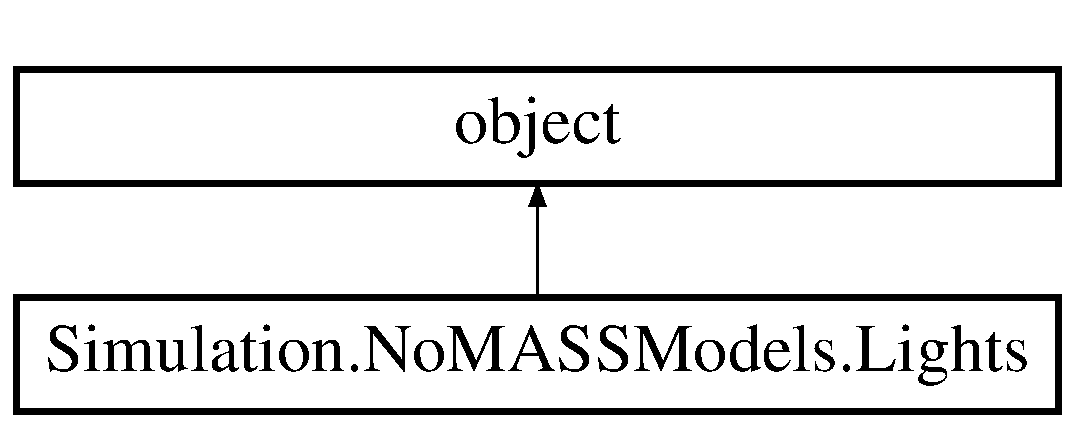
\includegraphics[height=2.000000cm]{class_c_simulation_1_1_simulation_1_1_no_m_a_s_s_models_1_1_lights}
\end{center}
\end{figure}
\subsection*{Public Member Functions}
\begin{DoxyCompactItemize}
\item 
\mbox{\Hypertarget{class_c_simulation_1_1_simulation_1_1_no_m_a_s_s_models_1_1_lights_ae64f0875afe3067b97ba370b354b9213}\label{class_c_simulation_1_1_simulation_1_1_no_m_a_s_s_models_1_1_lights_ae64f0875afe3067b97ba370b354b9213}} 
def {\bfseries \+\_\+\+\_\+init\+\_\+\+\_\+} (self)
\end{DoxyCompactItemize}
\subsection*{Public Attributes}
\begin{DoxyCompactItemize}
\item 
\mbox{\Hypertarget{class_c_simulation_1_1_simulation_1_1_no_m_a_s_s_models_1_1_lights_a91b39549c797bd5646357c8b6eecad0f}\label{class_c_simulation_1_1_simulation_1_1_no_m_a_s_s_models_1_1_lights_a91b39549c797bd5646357c8b6eecad0f}} 
{\bfseries enabled}
\end{DoxyCompactItemize}


\subsection{Detailed Description}


Definition at line 162 of file C\+Simulation.\+py.



The documentation for this class was generated from the following file\+:\begin{DoxyCompactItemize}
\item 
C\+Simulation.\+py\end{DoxyCompactItemize}

\hypertarget{class_c_utils_1_1_utils_1_1_u_i_1_1_controls_1_1_lst_box}{}\section{Utils.\+U\+I.\+Controls.\+Lst\+Box Class Reference}
\label{class_c_utils_1_1_utils_1_1_u_i_1_1_controls_1_1_lst_box}\index{Utils.\+U\+I.\+Controls.\+Lst\+Box@{Utils.\+U\+I.\+Controls.\+Lst\+Box}}
Inheritance diagram for Utils.\+U\+I.\+Controls.\+Lst\+Box\+:\begin{figure}[H]
\begin{center}
\leavevmode
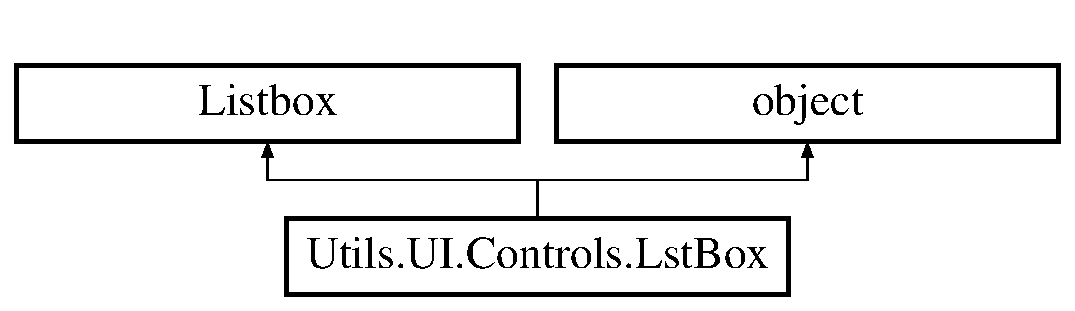
\includegraphics[height=2.000000cm]{class_c_utils_1_1_utils_1_1_u_i_1_1_controls_1_1_lst_box}
\end{center}
\end{figure}
\subsection*{Public Member Functions}
\begin{DoxyCompactItemize}
\item 
\mbox{\Hypertarget{class_c_utils_1_1_utils_1_1_u_i_1_1_controls_1_1_lst_box_a50195cb9bdd51876945eb2dd6fac4cac}\label{class_c_utils_1_1_utils_1_1_u_i_1_1_controls_1_1_lst_box_a50195cb9bdd51876945eb2dd6fac4cac}} 
def {\bfseries value} (self)
\item 
\mbox{\Hypertarget{class_c_utils_1_1_utils_1_1_u_i_1_1_controls_1_1_lst_box_a75bf740677ae53ef99707fdc9ede9f5b}\label{class_c_utils_1_1_utils_1_1_u_i_1_1_controls_1_1_lst_box_a75bf740677ae53ef99707fdc9ede9f5b}} 
def {\bfseries value} (self, values)
\item 
\mbox{\Hypertarget{class_c_utils_1_1_utils_1_1_u_i_1_1_controls_1_1_lst_box_a9bb637c47bf87426deb6e0821e31c15f}\label{class_c_utils_1_1_utils_1_1_u_i_1_1_controls_1_1_lst_box_a9bb637c47bf87426deb6e0821e31c15f}} 
def {\bfseries clear\+Selection} (self)
\item 
\mbox{\Hypertarget{class_c_utils_1_1_utils_1_1_u_i_1_1_controls_1_1_lst_box_a6726595c6381657ea6d43634eb6f1acb}\label{class_c_utils_1_1_utils_1_1_u_i_1_1_controls_1_1_lst_box_a6726595c6381657ea6d43634eb6f1acb}} 
def {\bfseries selected\+Values} (self)
\item 
\mbox{\Hypertarget{class_c_utils_1_1_utils_1_1_u_i_1_1_controls_1_1_lst_box_a0655f728fca2412c729fcae92722075e}\label{class_c_utils_1_1_utils_1_1_u_i_1_1_controls_1_1_lst_box_a0655f728fca2412c729fcae92722075e}} 
def {\bfseries selected\+Values} (self, list\+Of\+Values)
\item 
\mbox{\Hypertarget{class_c_utils_1_1_utils_1_1_u_i_1_1_controls_1_1_lst_box_afea4102108f673b1bc00df55095c7068}\label{class_c_utils_1_1_utils_1_1_u_i_1_1_controls_1_1_lst_box_afea4102108f673b1bc00df55095c7068}} 
def {\bfseries refresh\+Selection} (self)
\item 
\mbox{\Hypertarget{class_c_utils_1_1_utils_1_1_u_i_1_1_controls_1_1_lst_box_a1d458e4e6adb2f8a9a0af8bc280af7c8}\label{class_c_utils_1_1_utils_1_1_u_i_1_1_controls_1_1_lst_box_a1d458e4e6adb2f8a9a0af8bc280af7c8}} 
def {\bfseries On\+Select} (self, event=None)
\item 
\mbox{\Hypertarget{class_c_utils_1_1_utils_1_1_u_i_1_1_controls_1_1_lst_box_a0c5bac0610bebbd9b115f85e9a9fba36}\label{class_c_utils_1_1_utils_1_1_u_i_1_1_controls_1_1_lst_box_a0c5bac0610bebbd9b115f85e9a9fba36}} 
def {\bfseries \+\_\+\+\_\+init\+\_\+\+\_\+} (self, master, sort\+List=False, list=\{\}, args, kwargs)
\end{DoxyCompactItemize}
\subsection*{Public Attributes}
\begin{DoxyCompactItemize}
\item 
\mbox{\Hypertarget{class_c_utils_1_1_utils_1_1_u_i_1_1_controls_1_1_lst_box_a6bbb80367a84ef6bc36dcf82df1fea55}\label{class_c_utils_1_1_utils_1_1_u_i_1_1_controls_1_1_lst_box_a6bbb80367a84ef6bc36dcf82df1fea55}} 
{\bfseries list}
\item 
\mbox{\Hypertarget{class_c_utils_1_1_utils_1_1_u_i_1_1_controls_1_1_lst_box_a05b7a6fa81010873e4d6d46d3f7c1800}\label{class_c_utils_1_1_utils_1_1_u_i_1_1_controls_1_1_lst_box_a05b7a6fa81010873e4d6d46d3f7c1800}} 
{\bfseries sort\+List}
\end{DoxyCompactItemize}


\subsection{Detailed Description}


Definition at line 650 of file C\+Utils.\+py.



The documentation for this class was generated from the following file\+:\begin{DoxyCompactItemize}
\item 
C\+Utils.\+py\end{DoxyCompactItemize}

\hypertarget{class_c_simulation_1_1_simulation_1_1_no_m_a_s_s_models}{}\section{Simulation.\+No\+M\+A\+S\+S\+Models Class Reference}
\label{class_c_simulation_1_1_simulation_1_1_no_m_a_s_s_models}\index{Simulation.\+No\+M\+A\+S\+S\+Models@{Simulation.\+No\+M\+A\+S\+S\+Models}}
Inheritance diagram for Simulation.\+No\+M\+A\+S\+S\+Models\+:\begin{figure}[H]
\begin{center}
\leavevmode
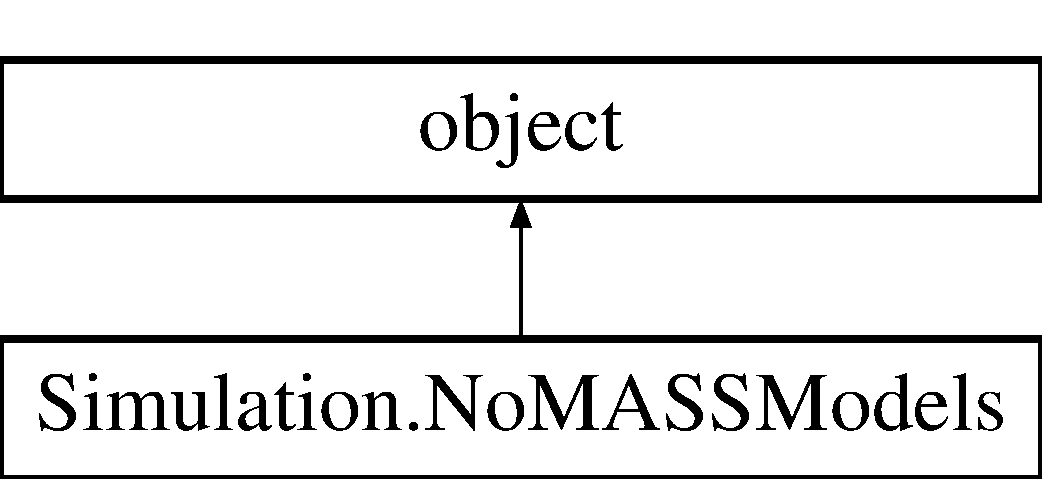
\includegraphics[height=2.000000cm]{class_c_simulation_1_1_simulation_1_1_no_m_a_s_s_models}
\end{center}
\end{figure}
\subsection*{Classes}
\begin{DoxyCompactItemize}
\item 
class \hyperlink{class_c_simulation_1_1_simulation_1_1_no_m_a_s_s_models_1_1_agent_heat_gains}{Agent\+Heat\+Gains}
\item 
class \hyperlink{class_c_simulation_1_1_simulation_1_1_no_m_a_s_s_models_1_1_heating}{Heating}
\item 
class \hyperlink{class_c_simulation_1_1_simulation_1_1_no_m_a_s_s_models_1_1_lights}{Lights}
\item 
class \hyperlink{class_c_simulation_1_1_simulation_1_1_no_m_a_s_s_models_1_1_presence}{Presence}
\item 
class \hyperlink{class_c_simulation_1_1_simulation_1_1_no_m_a_s_s_models_1_1_shades}{Shades}
\item 
class \hyperlink{class_c_simulation_1_1_simulation_1_1_no_m_a_s_s_models_1_1_windows}{Windows}
\end{DoxyCompactItemize}
\subsection*{Public Member Functions}
\begin{DoxyCompactItemize}
\item 
\mbox{\Hypertarget{class_c_simulation_1_1_simulation_1_1_no_m_a_s_s_models_ae64f0875afe3067b97ba370b354b9213}\label{class_c_simulation_1_1_simulation_1_1_no_m_a_s_s_models_ae64f0875afe3067b97ba370b354b9213}} 
def {\bfseries \+\_\+\+\_\+init\+\_\+\+\_\+} (self)
\end{DoxyCompactItemize}
\subsection*{Public Attributes}
\begin{DoxyCompactItemize}
\item 
\mbox{\Hypertarget{class_c_simulation_1_1_simulation_1_1_no_m_a_s_s_models_aff626664e93a8cb2aea6c0c33dbe72e9}\label{class_c_simulation_1_1_simulation_1_1_no_m_a_s_s_models_aff626664e93a8cb2aea6c0c33dbe72e9}} 
{\bfseries presence}
\item 
\mbox{\Hypertarget{class_c_simulation_1_1_simulation_1_1_no_m_a_s_s_models_a9364632a9ecc72c4ccec5a0db539657d}\label{class_c_simulation_1_1_simulation_1_1_no_m_a_s_s_models_a9364632a9ecc72c4ccec5a0db539657d}} 
{\bfseries lights}
\item 
\mbox{\Hypertarget{class_c_simulation_1_1_simulation_1_1_no_m_a_s_s_models_a099868ea758a9772c632b7883992a656}\label{class_c_simulation_1_1_simulation_1_1_no_m_a_s_s_models_a099868ea758a9772c632b7883992a656}} 
{\bfseries agent\+Heat\+Gains}
\item 
\mbox{\Hypertarget{class_c_simulation_1_1_simulation_1_1_no_m_a_s_s_models_afdb59a198434ba9fafeaea8a401498d1}\label{class_c_simulation_1_1_simulation_1_1_no_m_a_s_s_models_afdb59a198434ba9fafeaea8a401498d1}} 
{\bfseries heating}
\item 
\mbox{\Hypertarget{class_c_simulation_1_1_simulation_1_1_no_m_a_s_s_models_a836fa8579b25f4eb7c5b634cee3d6a54}\label{class_c_simulation_1_1_simulation_1_1_no_m_a_s_s_models_a836fa8579b25f4eb7c5b634cee3d6a54}} 
{\bfseries windows}
\item 
\mbox{\Hypertarget{class_c_simulation_1_1_simulation_1_1_no_m_a_s_s_models_a96ff58a0d53420486f2da9f07122e085}\label{class_c_simulation_1_1_simulation_1_1_no_m_a_s_s_models_a96ff58a0d53420486f2da9f07122e085}} 
{\bfseries shades}
\end{DoxyCompactItemize}


\subsection{Detailed Description}


Definition at line 154 of file C\+Simulation.\+py.



The documentation for this class was generated from the following file\+:\begin{DoxyCompactItemize}
\item 
C\+Simulation.\+py\end{DoxyCompactItemize}

\hypertarget{class_c_simulation_1_1_simulation_1_1_building_1_1_occupant}{}\section{Simulation.\+Building.\+Occupant Class Reference}
\label{class_c_simulation_1_1_simulation_1_1_building_1_1_occupant}\index{Simulation.\+Building.\+Occupant@{Simulation.\+Building.\+Occupant}}
Inheritance diagram for Simulation.\+Building.\+Occupant\+:\begin{figure}[H]
\begin{center}
\leavevmode
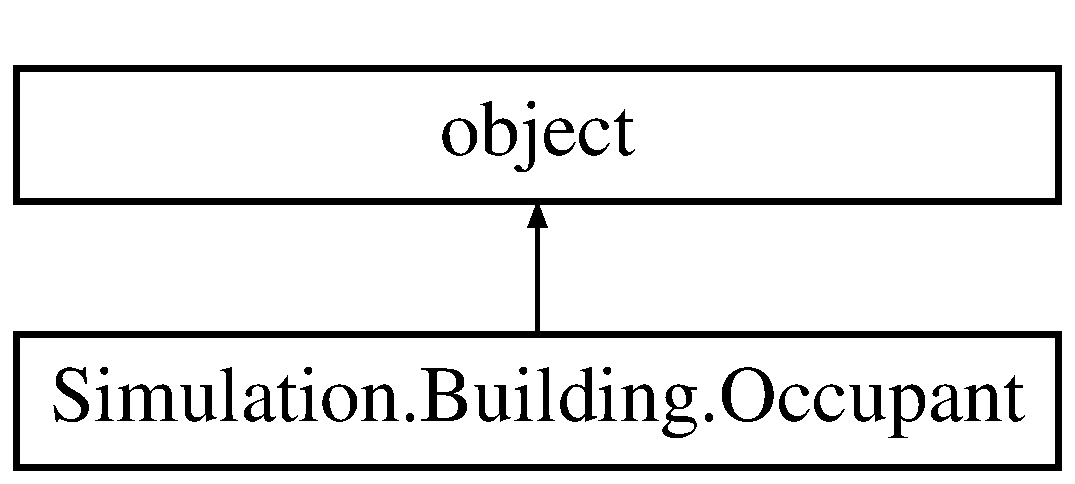
\includegraphics[height=2.000000cm]{class_c_simulation_1_1_simulation_1_1_building_1_1_occupant}
\end{center}
\end{figure}
\subsection*{Classes}
\begin{DoxyCompactItemize}
\item 
class \hyperlink{class_c_simulation_1_1_simulation_1_1_building_1_1_occupant_1_1_profile}{Profile}
\end{DoxyCompactItemize}
\subsection*{Public Member Functions}
\begin{DoxyCompactItemize}
\item 
\mbox{\Hypertarget{class_c_simulation_1_1_simulation_1_1_building_1_1_occupant_a4d48efcfaf9fc91f267e7cf2ba652d49}\label{class_c_simulation_1_1_simulation_1_1_building_1_1_occupant_a4d48efcfaf9fc91f267e7cf2ba652d49}} 
def {\bfseries \+\_\+\+\_\+init\+\_\+\+\_\+} (self, id=0, name=\textquotesingle{}\textquotesingle{}, description=\textquotesingle{}\textquotesingle{}, category\+ID=\textquotesingle{}\textquotesingle{}, category=\textquotesingle{}\textquotesingle{}, region\+ID=\textquotesingle{}\textquotesingle{}, region=\textquotesingle{}\textquotesingle{}, sector\+ID=\textquotesingle{}\textquotesingle{}, sector=\textquotesingle{}\textquotesingle{}, zone\+Id=\textquotesingle{}\textquotesingle{}, zone=\textquotesingle{}\textquotesingle{}, power=0, window\+Id=\textquotesingle{}\textquotesingle{}, window=\textquotesingle{}\textquotesingle{}, shade\+Id=\textquotesingle{}\textquotesingle{}, shade=\textquotesingle{}\textquotesingle{}, activity\+Id=\textquotesingle{}\textquotesingle{}, sex=\textquotesingle{}\textquotesingle{}, family\+ID=\textquotesingle{}\textquotesingle{}, education\+ID=\textquotesingle{}\textquotesingle{}, age\+Group=\textquotesingle{}\textquotesingle{}, own\+Computer=False, is\+Retired=False, is\+Married=False, is\+Un\+Employed=False)
\end{DoxyCompactItemize}
\subsection*{Public Attributes}
\begin{DoxyCompactItemize}
\item 
\mbox{\Hypertarget{class_c_simulation_1_1_simulation_1_1_building_1_1_occupant_ab72439091fb747e45522316f94689f0d}\label{class_c_simulation_1_1_simulation_1_1_building_1_1_occupant_ab72439091fb747e45522316f94689f0d}} 
{\bfseries uuid}
\item 
\mbox{\Hypertarget{class_c_simulation_1_1_simulation_1_1_building_1_1_occupant_acf2488b95c97e0378c9bf49de3b50f28}\label{class_c_simulation_1_1_simulation_1_1_building_1_1_occupant_acf2488b95c97e0378c9bf49de3b50f28}} 
{\bfseries id}
\item 
\mbox{\Hypertarget{class_c_simulation_1_1_simulation_1_1_building_1_1_occupant_ab74e6bf80237ddc4109968cedc58c151}\label{class_c_simulation_1_1_simulation_1_1_building_1_1_occupant_ab74e6bf80237ddc4109968cedc58c151}} 
{\bfseries name}
\item 
\mbox{\Hypertarget{class_c_simulation_1_1_simulation_1_1_building_1_1_occupant_a2661f439a4a94ffdcd5e47ae1da0bb1d}\label{class_c_simulation_1_1_simulation_1_1_building_1_1_occupant_a2661f439a4a94ffdcd5e47ae1da0bb1d}} 
{\bfseries description}
\item 
\mbox{\Hypertarget{class_c_simulation_1_1_simulation_1_1_building_1_1_occupant_a571cea1c26ae775da0baee0011a37438}\label{class_c_simulation_1_1_simulation_1_1_building_1_1_occupant_a571cea1c26ae775da0baee0011a37438}} 
{\bfseries category\+ID}
\item 
\mbox{\Hypertarget{class_c_simulation_1_1_simulation_1_1_building_1_1_occupant_a71494cb32e3acaab23cde05f1136df5e}\label{class_c_simulation_1_1_simulation_1_1_building_1_1_occupant_a71494cb32e3acaab23cde05f1136df5e}} 
{\bfseries category}
\item 
\mbox{\Hypertarget{class_c_simulation_1_1_simulation_1_1_building_1_1_occupant_a81760431d923bf4a1498c8de4c791862}\label{class_c_simulation_1_1_simulation_1_1_building_1_1_occupant_a81760431d923bf4a1498c8de4c791862}} 
{\bfseries region\+ID}
\item 
\mbox{\Hypertarget{class_c_simulation_1_1_simulation_1_1_building_1_1_occupant_a1b9edddb3735d131c67e9e824f07c402}\label{class_c_simulation_1_1_simulation_1_1_building_1_1_occupant_a1b9edddb3735d131c67e9e824f07c402}} 
{\bfseries region}
\item 
\mbox{\Hypertarget{class_c_simulation_1_1_simulation_1_1_building_1_1_occupant_ade42cbd183be4d1470fcd2860b5f6299}\label{class_c_simulation_1_1_simulation_1_1_building_1_1_occupant_ade42cbd183be4d1470fcd2860b5f6299}} 
{\bfseries sector\+ID}
\item 
\mbox{\Hypertarget{class_c_simulation_1_1_simulation_1_1_building_1_1_occupant_a7b1f19af9a2a259dfb128f8a76d930cb}\label{class_c_simulation_1_1_simulation_1_1_building_1_1_occupant_a7b1f19af9a2a259dfb128f8a76d930cb}} 
{\bfseries sector}
\item 
\mbox{\Hypertarget{class_c_simulation_1_1_simulation_1_1_building_1_1_occupant_a1fb3b1c128f08902cf8bb779ca84a8a7}\label{class_c_simulation_1_1_simulation_1_1_building_1_1_occupant_a1fb3b1c128f08902cf8bb779ca84a8a7}} 
{\bfseries zone\+Id}
\item 
\mbox{\Hypertarget{class_c_simulation_1_1_simulation_1_1_building_1_1_occupant_a828b8f8a58cd9813deb365aab404c850}\label{class_c_simulation_1_1_simulation_1_1_building_1_1_occupant_a828b8f8a58cd9813deb365aab404c850}} 
{\bfseries zone}
\item 
\mbox{\Hypertarget{class_c_simulation_1_1_simulation_1_1_building_1_1_occupant_a4aacd7f6a06e4071d328a3b2c9986701}\label{class_c_simulation_1_1_simulation_1_1_building_1_1_occupant_a4aacd7f6a06e4071d328a3b2c9986701}} 
{\bfseries power}
\item 
\mbox{\Hypertarget{class_c_simulation_1_1_simulation_1_1_building_1_1_occupant_a885f33c2f0f9d324955b06fcd3fb347d}\label{class_c_simulation_1_1_simulation_1_1_building_1_1_occupant_a885f33c2f0f9d324955b06fcd3fb347d}} 
{\bfseries window\+Id}
\item 
\mbox{\Hypertarget{class_c_simulation_1_1_simulation_1_1_building_1_1_occupant_a04a8a2bbfa9c15500892b8e5033d625b}\label{class_c_simulation_1_1_simulation_1_1_building_1_1_occupant_a04a8a2bbfa9c15500892b8e5033d625b}} 
{\bfseries window}
\item 
\mbox{\Hypertarget{class_c_simulation_1_1_simulation_1_1_building_1_1_occupant_a470c57d249cc6688d997e0d83be5189b}\label{class_c_simulation_1_1_simulation_1_1_building_1_1_occupant_a470c57d249cc6688d997e0d83be5189b}} 
{\bfseries shade\+Id}
\item 
\mbox{\Hypertarget{class_c_simulation_1_1_simulation_1_1_building_1_1_occupant_ae051ab0c565c3f206169ccfb187c4f90}\label{class_c_simulation_1_1_simulation_1_1_building_1_1_occupant_ae051ab0c565c3f206169ccfb187c4f90}} 
{\bfseries shade}
\item 
\mbox{\Hypertarget{class_c_simulation_1_1_simulation_1_1_building_1_1_occupant_a8f71c12055a15725c62d6a7ff32bed61}\label{class_c_simulation_1_1_simulation_1_1_building_1_1_occupant_a8f71c12055a15725c62d6a7ff32bed61}} 
{\bfseries activity\+Id}
\item 
\mbox{\Hypertarget{class_c_simulation_1_1_simulation_1_1_building_1_1_occupant_aa4826dcd193b4161365d7457e67da538}\label{class_c_simulation_1_1_simulation_1_1_building_1_1_occupant_aa4826dcd193b4161365d7457e67da538}} 
{\bfseries sex}
\item 
\mbox{\Hypertarget{class_c_simulation_1_1_simulation_1_1_building_1_1_occupant_ac1ce759a8faf1379a47b12486f9870a6}\label{class_c_simulation_1_1_simulation_1_1_building_1_1_occupant_ac1ce759a8faf1379a47b12486f9870a6}} 
{\bfseries family\+ID}
\item 
\mbox{\Hypertarget{class_c_simulation_1_1_simulation_1_1_building_1_1_occupant_a70b611151951af5deb863b2e95f9bb2a}\label{class_c_simulation_1_1_simulation_1_1_building_1_1_occupant_a70b611151951af5deb863b2e95f9bb2a}} 
{\bfseries education\+ID}
\item 
\mbox{\Hypertarget{class_c_simulation_1_1_simulation_1_1_building_1_1_occupant_a447f23cda1c2bdbc59a363452a231cca}\label{class_c_simulation_1_1_simulation_1_1_building_1_1_occupant_a447f23cda1c2bdbc59a363452a231cca}} 
{\bfseries age\+Group}
\item 
\mbox{\Hypertarget{class_c_simulation_1_1_simulation_1_1_building_1_1_occupant_a7a6fe25bfc965efce2ae2a9a5b1617b9}\label{class_c_simulation_1_1_simulation_1_1_building_1_1_occupant_a7a6fe25bfc965efce2ae2a9a5b1617b9}} 
{\bfseries own\+Computer}
\item 
\mbox{\Hypertarget{class_c_simulation_1_1_simulation_1_1_building_1_1_occupant_a48bfa9c03f920222617ef3cd7df804f0}\label{class_c_simulation_1_1_simulation_1_1_building_1_1_occupant_a48bfa9c03f920222617ef3cd7df804f0}} 
{\bfseries is\+Retired}
\item 
\mbox{\Hypertarget{class_c_simulation_1_1_simulation_1_1_building_1_1_occupant_ab82d3f752eab0bf656cf4ab2a33f81ac}\label{class_c_simulation_1_1_simulation_1_1_building_1_1_occupant_ab82d3f752eab0bf656cf4ab2a33f81ac}} 
{\bfseries is\+Married}
\item 
\mbox{\Hypertarget{class_c_simulation_1_1_simulation_1_1_building_1_1_occupant_a40bcaf70ef5162060ed12a883c1c40f2}\label{class_c_simulation_1_1_simulation_1_1_building_1_1_occupant_a40bcaf70ef5162060ed12a883c1c40f2}} 
{\bfseries is\+Un\+Employed}
\item 
\mbox{\Hypertarget{class_c_simulation_1_1_simulation_1_1_building_1_1_occupant_a7667610e670e037bd84c42dadbfbaa30}\label{class_c_simulation_1_1_simulation_1_1_building_1_1_occupant_a7667610e670e037bd84c42dadbfbaa30}} 
{\bfseries profile}
\end{DoxyCompactItemize}


\subsection{Detailed Description}


Definition at line 45 of file C\+Simulation.\+py.



The documentation for this class was generated from the following file\+:\begin{DoxyCompactItemize}
\item 
C\+Simulation.\+py\end{DoxyCompactItemize}

\hypertarget{class_c_simulation_1_1_simulation_1_1_no_m_a_s_s_models_1_1_presence}{}\section{Simulation.\+No\+M\+A\+S\+S\+Models.\+Presence Class Reference}
\label{class_c_simulation_1_1_simulation_1_1_no_m_a_s_s_models_1_1_presence}\index{Simulation.\+No\+M\+A\+S\+S\+Models.\+Presence@{Simulation.\+No\+M\+A\+S\+S\+Models.\+Presence}}
Inheritance diagram for Simulation.\+No\+M\+A\+S\+S\+Models.\+Presence\+:\begin{figure}[H]
\begin{center}
\leavevmode
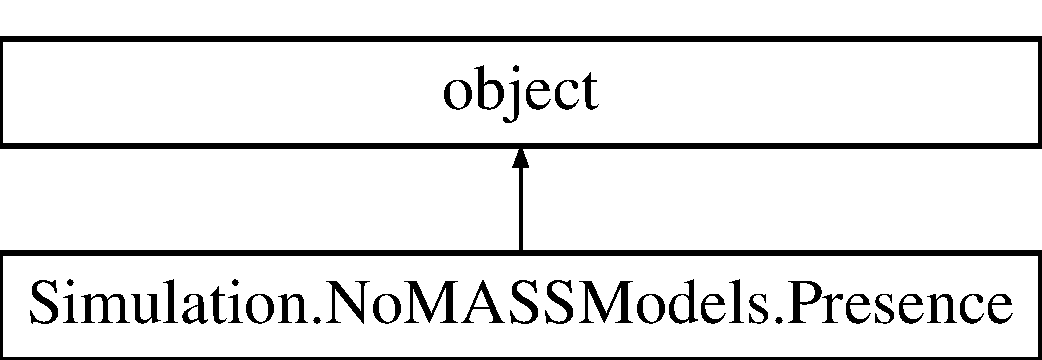
\includegraphics[height=2.000000cm]{class_c_simulation_1_1_simulation_1_1_no_m_a_s_s_models_1_1_presence}
\end{center}
\end{figure}
\subsection*{Public Member Functions}
\begin{DoxyCompactItemize}
\item 
\mbox{\Hypertarget{class_c_simulation_1_1_simulation_1_1_no_m_a_s_s_models_1_1_presence_ae64f0875afe3067b97ba370b354b9213}\label{class_c_simulation_1_1_simulation_1_1_no_m_a_s_s_models_1_1_presence_ae64f0875afe3067b97ba370b354b9213}} 
def {\bfseries \+\_\+\+\_\+init\+\_\+\+\_\+} (self)
\end{DoxyCompactItemize}
\subsection*{Public Attributes}
\begin{DoxyCompactItemize}
\item 
\mbox{\Hypertarget{class_c_simulation_1_1_simulation_1_1_no_m_a_s_s_models_1_1_presence_a91b39549c797bd5646357c8b6eecad0f}\label{class_c_simulation_1_1_simulation_1_1_no_m_a_s_s_models_1_1_presence_a91b39549c797bd5646357c8b6eecad0f}} 
{\bfseries enabled}
\end{DoxyCompactItemize}


\subsection{Detailed Description}


Definition at line 156 of file C\+Simulation.\+py.



The documentation for this class was generated from the following file\+:\begin{DoxyCompactItemize}
\item 
C\+Simulation.\+py\end{DoxyCompactItemize}

\hypertarget{class_c_simulation_1_1_simulation_1_1_building_1_1_occupant_1_1_profile}{}\section{Simulation.\+Building.\+Occupant.\+Profile Class Reference}
\label{class_c_simulation_1_1_simulation_1_1_building_1_1_occupant_1_1_profile}\index{Simulation.\+Building.\+Occupant.\+Profile@{Simulation.\+Building.\+Occupant.\+Profile}}
Inheritance diagram for Simulation.\+Building.\+Occupant.\+Profile\+:\begin{figure}[H]
\begin{center}
\leavevmode
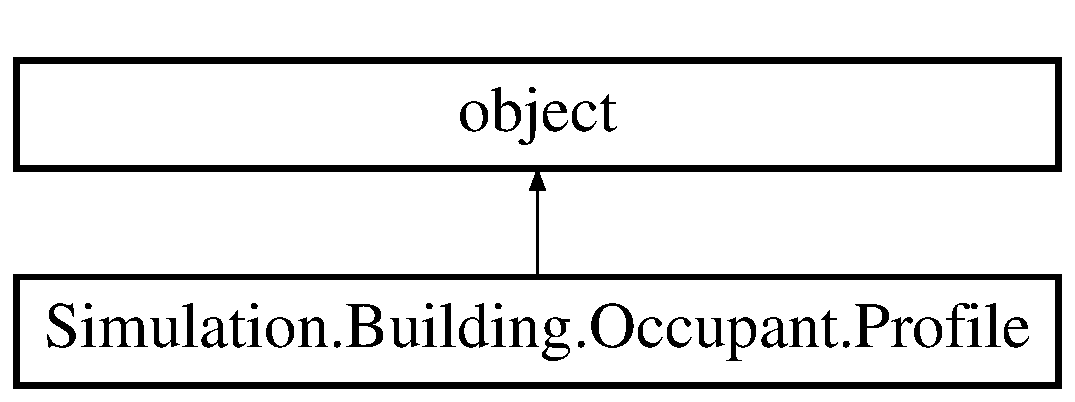
\includegraphics[height=2.000000cm]{class_c_simulation_1_1_simulation_1_1_building_1_1_occupant_1_1_profile}
\end{center}
\end{figure}
\subsection*{Public Member Functions}
\begin{DoxyCompactItemize}
\item 
\mbox{\Hypertarget{class_c_simulation_1_1_simulation_1_1_building_1_1_occupant_1_1_profile_ae64f0875afe3067b97ba370b354b9213}\label{class_c_simulation_1_1_simulation_1_1_building_1_1_occupant_1_1_profile_ae64f0875afe3067b97ba370b354b9213}} 
def {\bfseries \+\_\+\+\_\+init\+\_\+\+\_\+} (self)
\end{DoxyCompactItemize}
\subsection*{Public Attributes}
\begin{DoxyCompactItemize}
\item 
\mbox{\Hypertarget{class_c_simulation_1_1_simulation_1_1_building_1_1_occupant_1_1_profile_a094c367727273b4da2b960ca3b3edc06}\label{class_c_simulation_1_1_simulation_1_1_building_1_1_occupant_1_1_profile_a094c367727273b4da2b960ca3b3edc06}} 
{\bfseries ID}
\item 
\mbox{\Hypertarget{class_c_simulation_1_1_simulation_1_1_building_1_1_occupant_1_1_profile_a79ce83c7ce1b58bb61a61b647deb3ecc}\label{class_c_simulation_1_1_simulation_1_1_building_1_1_occupant_1_1_profile_a79ce83c7ce1b58bb61a61b647deb3ecc}} 
{\bfseries template}
\item 
\mbox{\Hypertarget{class_c_simulation_1_1_simulation_1_1_building_1_1_occupant_1_1_profile_a3ab88cae70b7ba3957ddca6b176e3efb}\label{class_c_simulation_1_1_simulation_1_1_building_1_1_occupant_1_1_profile_a3ab88cae70b7ba3957ddca6b176e3efb}} 
{\bfseries monday}
\item 
\mbox{\Hypertarget{class_c_simulation_1_1_simulation_1_1_building_1_1_occupant_1_1_profile_ae18d81b329b6533e55d227d8c6167ba7}\label{class_c_simulation_1_1_simulation_1_1_building_1_1_occupant_1_1_profile_ae18d81b329b6533e55d227d8c6167ba7}} 
{\bfseries tuesday}
\item 
\mbox{\Hypertarget{class_c_simulation_1_1_simulation_1_1_building_1_1_occupant_1_1_profile_a232ea81e2c28ad2aa675315f084371cd}\label{class_c_simulation_1_1_simulation_1_1_building_1_1_occupant_1_1_profile_a232ea81e2c28ad2aa675315f084371cd}} 
{\bfseries wednesday}
\item 
\mbox{\Hypertarget{class_c_simulation_1_1_simulation_1_1_building_1_1_occupant_1_1_profile_af780203eee7bba8eaa01524305037a08}\label{class_c_simulation_1_1_simulation_1_1_building_1_1_occupant_1_1_profile_af780203eee7bba8eaa01524305037a08}} 
{\bfseries thursday}
\item 
\mbox{\Hypertarget{class_c_simulation_1_1_simulation_1_1_building_1_1_occupant_1_1_profile_a26847417521ab033cc7de814eb4d0752}\label{class_c_simulation_1_1_simulation_1_1_building_1_1_occupant_1_1_profile_a26847417521ab033cc7de814eb4d0752}} 
{\bfseries friday}
\item 
\mbox{\Hypertarget{class_c_simulation_1_1_simulation_1_1_building_1_1_occupant_1_1_profile_adc2eb4ebb66e12ae0bbffcb2094c2c99}\label{class_c_simulation_1_1_simulation_1_1_building_1_1_occupant_1_1_profile_adc2eb4ebb66e12ae0bbffcb2094c2c99}} 
{\bfseries saturday}
\item 
\mbox{\Hypertarget{class_c_simulation_1_1_simulation_1_1_building_1_1_occupant_1_1_profile_a3a889f2f2eb0c1534bd7e364055f3067}\label{class_c_simulation_1_1_simulation_1_1_building_1_1_occupant_1_1_profile_a3a889f2f2eb0c1534bd7e364055f3067}} 
{\bfseries sunday}
\item 
\mbox{\Hypertarget{class_c_simulation_1_1_simulation_1_1_building_1_1_occupant_1_1_profile_aef92788f609145be9761ece7c139ed53}\label{class_c_simulation_1_1_simulation_1_1_building_1_1_occupant_1_1_profile_aef92788f609145be9761ece7c139ed53}} 
{\bfseries p0}
\item 
\mbox{\Hypertarget{class_c_simulation_1_1_simulation_1_1_building_1_1_occupant_1_1_profile_aa850ae5126b39a75859039aa84c3a577}\label{class_c_simulation_1_1_simulation_1_1_building_1_1_occupant_1_1_profile_aa850ae5126b39a75859039aa84c3a577}} 
{\bfseries p1}
\item 
\mbox{\Hypertarget{class_c_simulation_1_1_simulation_1_1_building_1_1_occupant_1_1_profile_a9099c7c12dde5f81f4d3ce261da3637c}\label{class_c_simulation_1_1_simulation_1_1_building_1_1_occupant_1_1_profile_a9099c7c12dde5f81f4d3ce261da3637c}} 
{\bfseries p2}
\item 
\mbox{\Hypertarget{class_c_simulation_1_1_simulation_1_1_building_1_1_occupant_1_1_profile_a5e2c8ac9008420e9ac3c008bef292c01}\label{class_c_simulation_1_1_simulation_1_1_building_1_1_occupant_1_1_profile_a5e2c8ac9008420e9ac3c008bef292c01}} 
{\bfseries p3}
\item 
\mbox{\Hypertarget{class_c_simulation_1_1_simulation_1_1_building_1_1_occupant_1_1_profile_a4d51e9c35c70dec46722c5f40c7cf8ce}\label{class_c_simulation_1_1_simulation_1_1_building_1_1_occupant_1_1_profile_a4d51e9c35c70dec46722c5f40c7cf8ce}} 
{\bfseries p4}
\item 
\mbox{\Hypertarget{class_c_simulation_1_1_simulation_1_1_building_1_1_occupant_1_1_profile_a6f3de1bc910f321194f78075114dd663}\label{class_c_simulation_1_1_simulation_1_1_building_1_1_occupant_1_1_profile_a6f3de1bc910f321194f78075114dd663}} 
{\bfseries p5}
\item 
\mbox{\Hypertarget{class_c_simulation_1_1_simulation_1_1_building_1_1_occupant_1_1_profile_a8c0cae8a45926b4c1a23d8fb8d209d14}\label{class_c_simulation_1_1_simulation_1_1_building_1_1_occupant_1_1_profile_a8c0cae8a45926b4c1a23d8fb8d209d14}} 
{\bfseries p6}
\item 
\mbox{\Hypertarget{class_c_simulation_1_1_simulation_1_1_building_1_1_occupant_1_1_profile_ae40956809eabff1a46883a4b4c6996f1}\label{class_c_simulation_1_1_simulation_1_1_building_1_1_occupant_1_1_profile_ae40956809eabff1a46883a4b4c6996f1}} 
{\bfseries p7}
\item 
\mbox{\Hypertarget{class_c_simulation_1_1_simulation_1_1_building_1_1_occupant_1_1_profile_aaa529075c33d0efbc96bf627f65e290e}\label{class_c_simulation_1_1_simulation_1_1_building_1_1_occupant_1_1_profile_aaa529075c33d0efbc96bf627f65e290e}} 
{\bfseries p8}
\item 
\mbox{\Hypertarget{class_c_simulation_1_1_simulation_1_1_building_1_1_occupant_1_1_profile_a7c2a7699b166f998d7eb415cf48fa6fb}\label{class_c_simulation_1_1_simulation_1_1_building_1_1_occupant_1_1_profile_a7c2a7699b166f998d7eb415cf48fa6fb}} 
{\bfseries p9}
\item 
\mbox{\Hypertarget{class_c_simulation_1_1_simulation_1_1_building_1_1_occupant_1_1_profile_a0cf13e73702be2b96c99e3ff7052bfa3}\label{class_c_simulation_1_1_simulation_1_1_building_1_1_occupant_1_1_profile_a0cf13e73702be2b96c99e3ff7052bfa3}} 
{\bfseries p10}
\item 
\mbox{\Hypertarget{class_c_simulation_1_1_simulation_1_1_building_1_1_occupant_1_1_profile_abbdc2339b8f2df35b4cadab6b0a83625}\label{class_c_simulation_1_1_simulation_1_1_building_1_1_occupant_1_1_profile_abbdc2339b8f2df35b4cadab6b0a83625}} 
{\bfseries p11}
\item 
\mbox{\Hypertarget{class_c_simulation_1_1_simulation_1_1_building_1_1_occupant_1_1_profile_ac76534ad8eaa17b96ced84a97b7ab077}\label{class_c_simulation_1_1_simulation_1_1_building_1_1_occupant_1_1_profile_ac76534ad8eaa17b96ced84a97b7ab077}} 
{\bfseries p12}
\item 
\mbox{\Hypertarget{class_c_simulation_1_1_simulation_1_1_building_1_1_occupant_1_1_profile_affdf9a617486710b128a559aab6412c5}\label{class_c_simulation_1_1_simulation_1_1_building_1_1_occupant_1_1_profile_affdf9a617486710b128a559aab6412c5}} 
{\bfseries p13}
\item 
\mbox{\Hypertarget{class_c_simulation_1_1_simulation_1_1_building_1_1_occupant_1_1_profile_a71e6f5f24403403ad664428b18c9cb9d}\label{class_c_simulation_1_1_simulation_1_1_building_1_1_occupant_1_1_profile_a71e6f5f24403403ad664428b18c9cb9d}} 
{\bfseries p14}
\item 
\mbox{\Hypertarget{class_c_simulation_1_1_simulation_1_1_building_1_1_occupant_1_1_profile_a74c3bb12772cdabfbe683844f657b8fe}\label{class_c_simulation_1_1_simulation_1_1_building_1_1_occupant_1_1_profile_a74c3bb12772cdabfbe683844f657b8fe}} 
{\bfseries p15}
\item 
\mbox{\Hypertarget{class_c_simulation_1_1_simulation_1_1_building_1_1_occupant_1_1_profile_afee7a5a5664f390e687f860e808201e8}\label{class_c_simulation_1_1_simulation_1_1_building_1_1_occupant_1_1_profile_afee7a5a5664f390e687f860e808201e8}} 
{\bfseries p16}
\item 
\mbox{\Hypertarget{class_c_simulation_1_1_simulation_1_1_building_1_1_occupant_1_1_profile_a063930b1d156024b2a1f54fd220f8c53}\label{class_c_simulation_1_1_simulation_1_1_building_1_1_occupant_1_1_profile_a063930b1d156024b2a1f54fd220f8c53}} 
{\bfseries p17}
\item 
\mbox{\Hypertarget{class_c_simulation_1_1_simulation_1_1_building_1_1_occupant_1_1_profile_ab469cf128cb8d16118624a2c98101f31}\label{class_c_simulation_1_1_simulation_1_1_building_1_1_occupant_1_1_profile_ab469cf128cb8d16118624a2c98101f31}} 
{\bfseries p18}
\item 
\mbox{\Hypertarget{class_c_simulation_1_1_simulation_1_1_building_1_1_occupant_1_1_profile_a4f94840fcc5ecdc9627379934eedee3b}\label{class_c_simulation_1_1_simulation_1_1_building_1_1_occupant_1_1_profile_a4f94840fcc5ecdc9627379934eedee3b}} 
{\bfseries p19}
\item 
\mbox{\Hypertarget{class_c_simulation_1_1_simulation_1_1_building_1_1_occupant_1_1_profile_a203b1175b809633a81f0b8b373a65a9d}\label{class_c_simulation_1_1_simulation_1_1_building_1_1_occupant_1_1_profile_a203b1175b809633a81f0b8b373a65a9d}} 
{\bfseries p20}
\item 
\mbox{\Hypertarget{class_c_simulation_1_1_simulation_1_1_building_1_1_occupant_1_1_profile_a7fcde72367d1274362d9c0ddfe62f721}\label{class_c_simulation_1_1_simulation_1_1_building_1_1_occupant_1_1_profile_a7fcde72367d1274362d9c0ddfe62f721}} 
{\bfseries p21}
\item 
\mbox{\Hypertarget{class_c_simulation_1_1_simulation_1_1_building_1_1_occupant_1_1_profile_a91c1dfa911ba0f5b7495d9f780955e6c}\label{class_c_simulation_1_1_simulation_1_1_building_1_1_occupant_1_1_profile_a91c1dfa911ba0f5b7495d9f780955e6c}} 
{\bfseries p22}
\item 
\mbox{\Hypertarget{class_c_simulation_1_1_simulation_1_1_building_1_1_occupant_1_1_profile_a09aac2df9e6628a1d4da2ea7e14671a4}\label{class_c_simulation_1_1_simulation_1_1_building_1_1_occupant_1_1_profile_a09aac2df9e6628a1d4da2ea7e14671a4}} 
{\bfseries p23}
\end{DoxyCompactItemize}


\subsection{Detailed Description}


Definition at line 46 of file C\+Simulation.\+py.



The documentation for this class was generated from the following file\+:\begin{DoxyCompactItemize}
\item 
C\+Simulation.\+py\end{DoxyCompactItemize}

\hypertarget{class_c_utils_1_1_utils_1_1_resources}{}\section{Utils.\+Resources Class Reference}
\label{class_c_utils_1_1_utils_1_1_resources}\index{Utils.\+Resources@{Utils.\+Resources}}
\subsection*{Classes}
\begin{DoxyCompactItemize}
\item 
class \hyperlink{class_c_utils_1_1_utils_1_1_resources_1_1_icons}{Icons}
\end{DoxyCompactItemize}


\subsection{Detailed Description}


Definition at line 975 of file C\+Utils.\+py.



The documentation for this class was generated from the following file\+:\begin{DoxyCompactItemize}
\item 
C\+Utils.\+py\end{DoxyCompactItemize}

\hypertarget{class_c_utils_1_1_utils_1_1_u_i_1_1_controls_1_1_scrollable_container}{}\section{Utils.\+U\+I.\+Controls.\+Scrollable\+Container Class Reference}
\label{class_c_utils_1_1_utils_1_1_u_i_1_1_controls_1_1_scrollable_container}\index{Utils.\+U\+I.\+Controls.\+Scrollable\+Container@{Utils.\+U\+I.\+Controls.\+Scrollable\+Container}}
Inheritance diagram for Utils.\+U\+I.\+Controls.\+Scrollable\+Container\+:\begin{figure}[H]
\begin{center}
\leavevmode
\includegraphics[height=2.000000cm]{class_c_utils_1_1_utils_1_1_u_i_1_1_controls_1_1_scrollable_container}
\end{center}
\end{figure}
\subsection*{Public Member Functions}
\begin{DoxyCompactItemize}
\item 
\mbox{\Hypertarget{class_c_utils_1_1_utils_1_1_u_i_1_1_controls_1_1_scrollable_container_a6032eb960798bc757a7e12247577f1a0}\label{class_c_utils_1_1_utils_1_1_u_i_1_1_controls_1_1_scrollable_container_a6032eb960798bc757a7e12247577f1a0}} 
def {\bfseries \+\_\+\+\_\+init\+\_\+\+\_\+} (self, parent, width=None, anchor=\char`\"{}n\char`\"{}, height=None, background=None, inner\+\_\+frame=tk.\+Frame, kw)
\item 
\mbox{\Hypertarget{class_c_utils_1_1_utils_1_1_u_i_1_1_controls_1_1_scrollable_container_abf5c3c9eaedca5fbf769d8f13daf83c8}\label{class_c_utils_1_1_utils_1_1_u_i_1_1_controls_1_1_scrollable_container_abf5c3c9eaedca5fbf769d8f13daf83c8}} 
def {\bfseries width} (self)
\item 
\mbox{\Hypertarget{class_c_utils_1_1_utils_1_1_u_i_1_1_controls_1_1_scrollable_container_a7f73ca3b6b06cab6bef4f2f023589144}\label{class_c_utils_1_1_utils_1_1_u_i_1_1_controls_1_1_scrollable_container_a7f73ca3b6b06cab6bef4f2f023589144}} 
def {\bfseries height} (self)
\item 
\mbox{\Hypertarget{class_c_utils_1_1_utils_1_1_u_i_1_1_controls_1_1_scrollable_container_a63bcca89b21de7ac9fbbab7d340f3945}\label{class_c_utils_1_1_utils_1_1_u_i_1_1_controls_1_1_scrollable_container_a63bcca89b21de7ac9fbbab7d340f3945}} 
def {\bfseries set\+Size} (self, width, height)
\item 
\mbox{\Hypertarget{class_c_utils_1_1_utils_1_1_u_i_1_1_controls_1_1_scrollable_container_aa8d0952e32b7b85a6191d8d413cb9f39}\label{class_c_utils_1_1_utils_1_1_u_i_1_1_controls_1_1_scrollable_container_aa8d0952e32b7b85a6191d8d413cb9f39}} 
def {\bfseries On\+Canvas\+\_\+\+Configure} (self, event)
\item 
\mbox{\Hypertarget{class_c_utils_1_1_utils_1_1_u_i_1_1_controls_1_1_scrollable_container_a67fdce12ad3df5d0b98fa9a0d409f6f3}\label{class_c_utils_1_1_utils_1_1_u_i_1_1_controls_1_1_scrollable_container_a67fdce12ad3df5d0b98fa9a0d409f6f3}} 
def {\bfseries update\+View\+Port} (self, new\+Width=None, new\+Height=None)
\end{DoxyCompactItemize}
\subsection*{Public Attributes}
\begin{DoxyCompactItemize}
\item 
\mbox{\Hypertarget{class_c_utils_1_1_utils_1_1_u_i_1_1_controls_1_1_scrollable_container_afa9e9838abb44338f7cbe41dc6f846d4}\label{class_c_utils_1_1_utils_1_1_u_i_1_1_controls_1_1_scrollable_container_afa9e9838abb44338f7cbe41dc6f846d4}} 
{\bfseries canvas}
\item 
\mbox{\Hypertarget{class_c_utils_1_1_utils_1_1_u_i_1_1_controls_1_1_scrollable_container_a43a0eb61826d461f73acda3ad80dbb04}\label{class_c_utils_1_1_utils_1_1_u_i_1_1_controls_1_1_scrollable_container_a43a0eb61826d461f73acda3ad80dbb04}} 
{\bfseries yscrollbar}
\item 
\mbox{\Hypertarget{class_c_utils_1_1_utils_1_1_u_i_1_1_controls_1_1_scrollable_container_a8ec2a9bb5b54d7e6266121686b2e9df1}\label{class_c_utils_1_1_utils_1_1_u_i_1_1_controls_1_1_scrollable_container_a8ec2a9bb5b54d7e6266121686b2e9df1}} 
{\bfseries xscrollbar}
\item 
\mbox{\Hypertarget{class_c_utils_1_1_utils_1_1_u_i_1_1_controls_1_1_scrollable_container_abeae1752984a7b01d65cdcde9c1a1126}\label{class_c_utils_1_1_utils_1_1_u_i_1_1_controls_1_1_scrollable_container_abeae1752984a7b01d65cdcde9c1a1126}} 
{\bfseries innerframe}
\end{DoxyCompactItemize}


\subsection{Detailed Description}


Definition at line 896 of file C\+Utils.\+py.



The documentation for this class was generated from the following file\+:\begin{DoxyCompactItemize}
\item 
C\+Utils.\+py\end{DoxyCompactItemize}

\hypertarget{class_c_utils_1_1_utils_1_1_u_i_1_1_controls_1_1_scrolled_tree_view}{}\section{Utils.\+U\+I.\+Controls.\+Scrolled\+Tree\+View Class Reference}
\label{class_c_utils_1_1_utils_1_1_u_i_1_1_controls_1_1_scrolled_tree_view}\index{Utils.\+U\+I.\+Controls.\+Scrolled\+Tree\+View@{Utils.\+U\+I.\+Controls.\+Scrolled\+Tree\+View}}
Inheritance diagram for Utils.\+U\+I.\+Controls.\+Scrolled\+Tree\+View\+:\begin{figure}[H]
\begin{center}
\leavevmode
\includegraphics[height=3.000000cm]{class_c_utils_1_1_utils_1_1_u_i_1_1_controls_1_1_scrolled_tree_view}
\end{center}
\end{figure}
\subsection*{Public Member Functions}
\begin{DoxyCompactItemize}
\item 
\mbox{\Hypertarget{class_c_utils_1_1_utils_1_1_u_i_1_1_controls_1_1_scrolled_tree_view_ae6645e6d34396c7c51b80d9b8f7d4ed1}\label{class_c_utils_1_1_utils_1_1_u_i_1_1_controls_1_1_scrolled_tree_view_ae6645e6d34396c7c51b80d9b8f7d4ed1}} 
def {\bfseries clear\+On\+Move} (self, event=None)
\item 
\mbox{\Hypertarget{class_c_utils_1_1_utils_1_1_u_i_1_1_controls_1_1_scrolled_tree_view_a508f7bacf9ccbf6610b5c16218ec1085}\label{class_c_utils_1_1_utils_1_1_u_i_1_1_controls_1_1_scrolled_tree_view_a508f7bacf9ccbf6610b5c16218ec1085}} 
def {\bfseries On\+Motion} (self, event)
\item 
\mbox{\Hypertarget{class_c_utils_1_1_utils_1_1_u_i_1_1_controls_1_1_scrolled_tree_view_aaf53b59f766d5d03501a9df01b054d75}\label{class_c_utils_1_1_utils_1_1_u_i_1_1_controls_1_1_scrolled_tree_view_aaf53b59f766d5d03501a9df01b054d75}} 
def {\bfseries show\+Tip} (self, item\+Id, text, event\+\_\+x, event\+\_\+y)
\item 
\mbox{\Hypertarget{class_c_utils_1_1_utils_1_1_u_i_1_1_controls_1_1_scrolled_tree_view_a42d1da3c0fa907a93351f3f6e3e7c864}\label{class_c_utils_1_1_utils_1_1_u_i_1_1_controls_1_1_scrolled_tree_view_a42d1da3c0fa907a93351f3f6e3e7c864}} 
def {\bfseries hide\+Tip} (self, event=None)
\item 
\mbox{\Hypertarget{class_c_utils_1_1_utils_1_1_u_i_1_1_controls_1_1_scrolled_tree_view_aa3be958b4753452478bab15ebbdc356b}\label{class_c_utils_1_1_utils_1_1_u_i_1_1_controls_1_1_scrolled_tree_view_aa3be958b4753452478bab15ebbdc356b}} 
def {\bfseries \+\_\+\+\_\+init\+\_\+\+\_\+} (self, master, kw)
\end{DoxyCompactItemize}
\subsection*{Public Attributes}
\begin{DoxyCompactItemize}
\item 
\mbox{\Hypertarget{class_c_utils_1_1_utils_1_1_u_i_1_1_controls_1_1_scrolled_tree_view_a6c622a9a7ebc7bbaabf43e1490b2ac1f}\label{class_c_utils_1_1_utils_1_1_u_i_1_1_controls_1_1_scrolled_tree_view_a6c622a9a7ebc7bbaabf43e1490b2ac1f}} 
{\bfseries last\+\_\+focus}
\item 
\mbox{\Hypertarget{class_c_utils_1_1_utils_1_1_u_i_1_1_controls_1_1_scrolled_tree_view_a5463352dcbbdaaeb782f0484b30f87f1}\label{class_c_utils_1_1_utils_1_1_u_i_1_1_controls_1_1_scrolled_tree_view_a5463352dcbbdaaeb782f0484b30f87f1}} 
{\bfseries tipwindow}
\item 
\mbox{\Hypertarget{class_c_utils_1_1_utils_1_1_u_i_1_1_controls_1_1_scrolled_tree_view_acf2488b95c97e0378c9bf49de3b50f28}\label{class_c_utils_1_1_utils_1_1_u_i_1_1_controls_1_1_scrolled_tree_view_acf2488b95c97e0378c9bf49de3b50f28}} 
{\bfseries id}
\item 
\mbox{\Hypertarget{class_c_utils_1_1_utils_1_1_u_i_1_1_controls_1_1_scrolled_tree_view_a9336ebf25087d91c818ee6e9ec29f8c1}\label{class_c_utils_1_1_utils_1_1_u_i_1_1_controls_1_1_scrolled_tree_view_a9336ebf25087d91c818ee6e9ec29f8c1}} 
{\bfseries x}
\item 
\mbox{\Hypertarget{class_c_utils_1_1_utils_1_1_u_i_1_1_controls_1_1_scrolled_tree_view_a2fb1c5cf58867b5bbc9a1b145a86f3a0}\label{class_c_utils_1_1_utils_1_1_u_i_1_1_controls_1_1_scrolled_tree_view_a2fb1c5cf58867b5bbc9a1b145a86f3a0}} 
{\bfseries y}
\item 
\mbox{\Hypertarget{class_c_utils_1_1_utils_1_1_u_i_1_1_controls_1_1_scrolled_tree_view_af575f17e6be3f269b86b041a60560dbf}\label{class_c_utils_1_1_utils_1_1_u_i_1_1_controls_1_1_scrolled_tree_view_af575f17e6be3f269b86b041a60560dbf}} 
{\bfseries text}
\item 
\mbox{\Hypertarget{class_c_utils_1_1_utils_1_1_u_i_1_1_controls_1_1_scrolled_tree_view_a5b16ea76b064935dd1a830d81ba2bac5}\label{class_c_utils_1_1_utils_1_1_u_i_1_1_controls_1_1_scrolled_tree_view_a5b16ea76b064935dd1a830d81ba2bac5}} 
{\bfseries show\+Tool\+Tip}
\item 
\mbox{\Hypertarget{class_c_utils_1_1_utils_1_1_u_i_1_1_controls_1_1_scrolled_tree_view_a030ecaa2a61b422a8ca7422403ad8c77}\label{class_c_utils_1_1_utils_1_1_u_i_1_1_controls_1_1_scrolled_tree_view_a030ecaa2a61b422a8ca7422403ad8c77}} 
{\bfseries container}
\end{DoxyCompactItemize}
\subsection*{Additional Inherited Members}


\subsection{Detailed Description}


Definition at line 786 of file C\+Utils.\+py.



The documentation for this class was generated from the following file\+:\begin{DoxyCompactItemize}
\item 
C\+Utils.\+py\end{DoxyCompactItemize}

\hypertarget{class_c_simulation_1_1_simulation_1_1_no_m_a_s_s_models_1_1_shades_1_1_shade}{}\section{Simulation.\+No\+M\+A\+S\+S\+Models.\+Shades.\+Shade Class Reference}
\label{class_c_simulation_1_1_simulation_1_1_no_m_a_s_s_models_1_1_shades_1_1_shade}\index{Simulation.\+No\+M\+A\+S\+S\+Models.\+Shades.\+Shade@{Simulation.\+No\+M\+A\+S\+S\+Models.\+Shades.\+Shade}}
Inheritance diagram for Simulation.\+No\+M\+A\+S\+S\+Models.\+Shades.\+Shade\+:\begin{figure}[H]
\begin{center}
\leavevmode
\includegraphics[height=2.000000cm]{class_c_simulation_1_1_simulation_1_1_no_m_a_s_s_models_1_1_shades_1_1_shade}
\end{center}
\end{figure}
\subsection*{Public Member Functions}
\begin{DoxyCompactItemize}
\item 
\mbox{\Hypertarget{class_c_simulation_1_1_simulation_1_1_no_m_a_s_s_models_1_1_shades_1_1_shade_a005f8f2d5acfee7d24d1aac6005a1e0a}\label{class_c_simulation_1_1_simulation_1_1_no_m_a_s_s_models_1_1_shades_1_1_shade_a005f8f2d5acfee7d24d1aac6005a1e0a}} 
def {\bfseries get\+Key} (self)
\item 
\mbox{\Hypertarget{class_c_simulation_1_1_simulation_1_1_no_m_a_s_s_models_1_1_shades_1_1_shade_aecfe92e74f185bbe044724fc20ff0e0e}\label{class_c_simulation_1_1_simulation_1_1_no_m_a_s_s_models_1_1_shades_1_1_shade_aecfe92e74f185bbe044724fc20ff0e0e}} 
def {\bfseries \+\_\+\+\_\+init\+\_\+\+\_\+} (self, id=0, name=\textquotesingle{}\textquotesingle{}, a01arr=0, b01inarr=0, b01sarr=0, a10arr=0, b10inarr=0, b10sarr=0, a01int=0, b01inint=0, b01sint=0, a10int=0, b10inint=0, b10sint=0, afullraise=0, boutfullraise=0, bsfullraise=0, bsfulllower=0, boutfulllower=0, afulllower=0, a\+S\+Flower=0, b\+S\+Flower=0, shapelower=0)
\item 
\mbox{\Hypertarget{class_c_simulation_1_1_simulation_1_1_no_m_a_s_s_models_1_1_shades_1_1_shade_a9a47563093dfc5ba12274b66e368920c}\label{class_c_simulation_1_1_simulation_1_1_no_m_a_s_s_models_1_1_shades_1_1_shade_a9a47563093dfc5ba12274b66e368920c}} 
def {\bfseries \+\_\+\+\_\+repr\+\_\+\+\_\+} (self)
\item 
\mbox{\Hypertarget{class_c_simulation_1_1_simulation_1_1_no_m_a_s_s_models_1_1_shades_1_1_shade_a157f9a5d3230b5fbbcb1391575ca1662}\label{class_c_simulation_1_1_simulation_1_1_no_m_a_s_s_models_1_1_shades_1_1_shade_a157f9a5d3230b5fbbcb1391575ca1662}} 
def {\bfseries \+\_\+\+\_\+cmp\+\_\+\+\_\+} (self, other)
\end{DoxyCompactItemize}
\subsection*{Public Attributes}
\begin{DoxyCompactItemize}
\item 
\mbox{\Hypertarget{class_c_simulation_1_1_simulation_1_1_no_m_a_s_s_models_1_1_shades_1_1_shade_acf2488b95c97e0378c9bf49de3b50f28}\label{class_c_simulation_1_1_simulation_1_1_no_m_a_s_s_models_1_1_shades_1_1_shade_acf2488b95c97e0378c9bf49de3b50f28}} 
{\bfseries id}
\item 
\mbox{\Hypertarget{class_c_simulation_1_1_simulation_1_1_no_m_a_s_s_models_1_1_shades_1_1_shade_ab74e6bf80237ddc4109968cedc58c151}\label{class_c_simulation_1_1_simulation_1_1_no_m_a_s_s_models_1_1_shades_1_1_shade_ab74e6bf80237ddc4109968cedc58c151}} 
{\bfseries name}
\item 
\mbox{\Hypertarget{class_c_simulation_1_1_simulation_1_1_no_m_a_s_s_models_1_1_shades_1_1_shade_ad4138a926b887cee1f1cb00cf7c0c0d8}\label{class_c_simulation_1_1_simulation_1_1_no_m_a_s_s_models_1_1_shades_1_1_shade_ad4138a926b887cee1f1cb00cf7c0c0d8}} 
{\bfseries a01arr}
\item 
\mbox{\Hypertarget{class_c_simulation_1_1_simulation_1_1_no_m_a_s_s_models_1_1_shades_1_1_shade_a642ea58b2a89e94a68a45fef0238d38d}\label{class_c_simulation_1_1_simulation_1_1_no_m_a_s_s_models_1_1_shades_1_1_shade_a642ea58b2a89e94a68a45fef0238d38d}} 
{\bfseries b01inarr}
\item 
\mbox{\Hypertarget{class_c_simulation_1_1_simulation_1_1_no_m_a_s_s_models_1_1_shades_1_1_shade_ae5137a043b834cbc48f539fe76b2d6c7}\label{class_c_simulation_1_1_simulation_1_1_no_m_a_s_s_models_1_1_shades_1_1_shade_ae5137a043b834cbc48f539fe76b2d6c7}} 
{\bfseries b01sarr}
\item 
\mbox{\Hypertarget{class_c_simulation_1_1_simulation_1_1_no_m_a_s_s_models_1_1_shades_1_1_shade_ab4adfe11143bf2076adf839b2cf15859}\label{class_c_simulation_1_1_simulation_1_1_no_m_a_s_s_models_1_1_shades_1_1_shade_ab4adfe11143bf2076adf839b2cf15859}} 
{\bfseries a10arr}
\item 
\mbox{\Hypertarget{class_c_simulation_1_1_simulation_1_1_no_m_a_s_s_models_1_1_shades_1_1_shade_ab6b0d3b1d8accc11623c4a6ffd1fa5ba}\label{class_c_simulation_1_1_simulation_1_1_no_m_a_s_s_models_1_1_shades_1_1_shade_ab6b0d3b1d8accc11623c4a6ffd1fa5ba}} 
{\bfseries b10inarr}
\item 
\mbox{\Hypertarget{class_c_simulation_1_1_simulation_1_1_no_m_a_s_s_models_1_1_shades_1_1_shade_a83b7000e6f87e51c070bc945e9133af7}\label{class_c_simulation_1_1_simulation_1_1_no_m_a_s_s_models_1_1_shades_1_1_shade_a83b7000e6f87e51c070bc945e9133af7}} 
{\bfseries b10sarr}
\item 
\mbox{\Hypertarget{class_c_simulation_1_1_simulation_1_1_no_m_a_s_s_models_1_1_shades_1_1_shade_ac6de2c7ea86ba3d4429acf25eeb13077}\label{class_c_simulation_1_1_simulation_1_1_no_m_a_s_s_models_1_1_shades_1_1_shade_ac6de2c7ea86ba3d4429acf25eeb13077}} 
{\bfseries a01int}
\item 
\mbox{\Hypertarget{class_c_simulation_1_1_simulation_1_1_no_m_a_s_s_models_1_1_shades_1_1_shade_a5b2b7bd2d91ffac2459813732c85ff8f}\label{class_c_simulation_1_1_simulation_1_1_no_m_a_s_s_models_1_1_shades_1_1_shade_a5b2b7bd2d91ffac2459813732c85ff8f}} 
{\bfseries b01inint}
\item 
\mbox{\Hypertarget{class_c_simulation_1_1_simulation_1_1_no_m_a_s_s_models_1_1_shades_1_1_shade_a1603d0fe11f74c954081209fa9a02bdd}\label{class_c_simulation_1_1_simulation_1_1_no_m_a_s_s_models_1_1_shades_1_1_shade_a1603d0fe11f74c954081209fa9a02bdd}} 
{\bfseries b01sint}
\item 
\mbox{\Hypertarget{class_c_simulation_1_1_simulation_1_1_no_m_a_s_s_models_1_1_shades_1_1_shade_a47a4ced31c152d89c2de210e07d72914}\label{class_c_simulation_1_1_simulation_1_1_no_m_a_s_s_models_1_1_shades_1_1_shade_a47a4ced31c152d89c2de210e07d72914}} 
{\bfseries a10int}
\item 
\mbox{\Hypertarget{class_c_simulation_1_1_simulation_1_1_no_m_a_s_s_models_1_1_shades_1_1_shade_a5192ca5056f4d4fa91c2959d624d2ca0}\label{class_c_simulation_1_1_simulation_1_1_no_m_a_s_s_models_1_1_shades_1_1_shade_a5192ca5056f4d4fa91c2959d624d2ca0}} 
{\bfseries b10inint}
\item 
\mbox{\Hypertarget{class_c_simulation_1_1_simulation_1_1_no_m_a_s_s_models_1_1_shades_1_1_shade_aaa7881ba7f71c2c9ea80e5360ceef07a}\label{class_c_simulation_1_1_simulation_1_1_no_m_a_s_s_models_1_1_shades_1_1_shade_aaa7881ba7f71c2c9ea80e5360ceef07a}} 
{\bfseries b10sint}
\item 
\mbox{\Hypertarget{class_c_simulation_1_1_simulation_1_1_no_m_a_s_s_models_1_1_shades_1_1_shade_a6dd8c5e61eafa019772f77effdb67be2}\label{class_c_simulation_1_1_simulation_1_1_no_m_a_s_s_models_1_1_shades_1_1_shade_a6dd8c5e61eafa019772f77effdb67be2}} 
{\bfseries afullraise}
\item 
\mbox{\Hypertarget{class_c_simulation_1_1_simulation_1_1_no_m_a_s_s_models_1_1_shades_1_1_shade_a74b1763a48cc2e108d60e7dd558d05b4}\label{class_c_simulation_1_1_simulation_1_1_no_m_a_s_s_models_1_1_shades_1_1_shade_a74b1763a48cc2e108d60e7dd558d05b4}} 
{\bfseries boutfullraise}
\item 
\mbox{\Hypertarget{class_c_simulation_1_1_simulation_1_1_no_m_a_s_s_models_1_1_shades_1_1_shade_a9a26ff9362f83e91d67d1392812b89a8}\label{class_c_simulation_1_1_simulation_1_1_no_m_a_s_s_models_1_1_shades_1_1_shade_a9a26ff9362f83e91d67d1392812b89a8}} 
{\bfseries bsfullraise}
\item 
\mbox{\Hypertarget{class_c_simulation_1_1_simulation_1_1_no_m_a_s_s_models_1_1_shades_1_1_shade_a0dab9492a1910f3dbef1e0ac57954ef9}\label{class_c_simulation_1_1_simulation_1_1_no_m_a_s_s_models_1_1_shades_1_1_shade_a0dab9492a1910f3dbef1e0ac57954ef9}} 
{\bfseries bsfulllower}
\item 
\mbox{\Hypertarget{class_c_simulation_1_1_simulation_1_1_no_m_a_s_s_models_1_1_shades_1_1_shade_a4bd43c964c14d7d83698718a3fd97407}\label{class_c_simulation_1_1_simulation_1_1_no_m_a_s_s_models_1_1_shades_1_1_shade_a4bd43c964c14d7d83698718a3fd97407}} 
{\bfseries boutfulllower}
\item 
\mbox{\Hypertarget{class_c_simulation_1_1_simulation_1_1_no_m_a_s_s_models_1_1_shades_1_1_shade_a03dbfc34573e6d7095a9b4c93e15f2d7}\label{class_c_simulation_1_1_simulation_1_1_no_m_a_s_s_models_1_1_shades_1_1_shade_a03dbfc34573e6d7095a9b4c93e15f2d7}} 
{\bfseries afulllower}
\item 
\mbox{\Hypertarget{class_c_simulation_1_1_simulation_1_1_no_m_a_s_s_models_1_1_shades_1_1_shade_a756f7dc07777dfdc9fd82deca77c1966}\label{class_c_simulation_1_1_simulation_1_1_no_m_a_s_s_models_1_1_shades_1_1_shade_a756f7dc07777dfdc9fd82deca77c1966}} 
{\bfseries a\+S\+Flower}
\item 
\mbox{\Hypertarget{class_c_simulation_1_1_simulation_1_1_no_m_a_s_s_models_1_1_shades_1_1_shade_a69a0472d1f1e0525e4b1a814ac547a45}\label{class_c_simulation_1_1_simulation_1_1_no_m_a_s_s_models_1_1_shades_1_1_shade_a69a0472d1f1e0525e4b1a814ac547a45}} 
{\bfseries b\+S\+Flower}
\item 
\mbox{\Hypertarget{class_c_simulation_1_1_simulation_1_1_no_m_a_s_s_models_1_1_shades_1_1_shade_af31bbc2a713476c8520b2af9e1423112}\label{class_c_simulation_1_1_simulation_1_1_no_m_a_s_s_models_1_1_shades_1_1_shade_af31bbc2a713476c8520b2af9e1423112}} 
{\bfseries shapelower}
\end{DoxyCompactItemize}


\subsection{Detailed Description}


Definition at line 259 of file C\+Simulation.\+py.



The documentation for this class was generated from the following file\+:\begin{DoxyCompactItemize}
\item 
C\+Simulation.\+py\end{DoxyCompactItemize}

\hypertarget{class_c_simulation_1_1_simulation_1_1_no_m_a_s_s_models_1_1_shades}{}\section{Simulation.\+No\+M\+A\+S\+S\+Models.\+Shades Class Reference}
\label{class_c_simulation_1_1_simulation_1_1_no_m_a_s_s_models_1_1_shades}\index{Simulation.\+No\+M\+A\+S\+S\+Models.\+Shades@{Simulation.\+No\+M\+A\+S\+S\+Models.\+Shades}}
Inheritance diagram for Simulation.\+No\+M\+A\+S\+S\+Models.\+Shades\+:\begin{figure}[H]
\begin{center}
\leavevmode
\includegraphics[height=2.000000cm]{class_c_simulation_1_1_simulation_1_1_no_m_a_s_s_models_1_1_shades}
\end{center}
\end{figure}
\subsection*{Classes}
\begin{DoxyCompactItemize}
\item 
class \hyperlink{class_c_simulation_1_1_simulation_1_1_no_m_a_s_s_models_1_1_shades_1_1_shade}{Shade}
\end{DoxyCompactItemize}
\subsection*{Public Member Functions}
\begin{DoxyCompactItemize}
\item 
\mbox{\Hypertarget{class_c_simulation_1_1_simulation_1_1_no_m_a_s_s_models_1_1_shades_ad149341d7d849ff957baee565b19c123}\label{class_c_simulation_1_1_simulation_1_1_no_m_a_s_s_models_1_1_shades_ad149341d7d849ff957baee565b19c123}} 
def {\bfseries clear} (self)
\item 
\mbox{\Hypertarget{class_c_simulation_1_1_simulation_1_1_no_m_a_s_s_models_1_1_shades_afeb95331c52b9ae001dbeacd1b58218f}\label{class_c_simulation_1_1_simulation_1_1_no_m_a_s_s_models_1_1_shades_afeb95331c52b9ae001dbeacd1b58218f}} 
def {\bfseries append} (self, obj\+Shade)
\item 
\mbox{\Hypertarget{class_c_simulation_1_1_simulation_1_1_no_m_a_s_s_models_1_1_shades_ae64f0875afe3067b97ba370b354b9213}\label{class_c_simulation_1_1_simulation_1_1_no_m_a_s_s_models_1_1_shades_ae64f0875afe3067b97ba370b354b9213}} 
def {\bfseries \+\_\+\+\_\+init\+\_\+\+\_\+} (self)
\end{DoxyCompactItemize}
\subsection*{Public Attributes}
\begin{DoxyCompactItemize}
\item 
\mbox{\Hypertarget{class_c_simulation_1_1_simulation_1_1_no_m_a_s_s_models_1_1_shades_a91b39549c797bd5646357c8b6eecad0f}\label{class_c_simulation_1_1_simulation_1_1_no_m_a_s_s_models_1_1_shades_a91b39549c797bd5646357c8b6eecad0f}} 
{\bfseries enabled}
\item 
\mbox{\Hypertarget{class_c_simulation_1_1_simulation_1_1_no_m_a_s_s_models_1_1_shades_a96ff58a0d53420486f2da9f07122e085}\label{class_c_simulation_1_1_simulation_1_1_no_m_a_s_s_models_1_1_shades_a96ff58a0d53420486f2da9f07122e085}} 
{\bfseries shades}
\end{DoxyCompactItemize}


\subsection{Detailed Description}


Definition at line 258 of file C\+Simulation.\+py.



The documentation for this class was generated from the following file\+:\begin{DoxyCompactItemize}
\item 
C\+Simulation.\+py\end{DoxyCompactItemize}

\hypertarget{class_c_simulation_1_1_simulation}{}\section{Simulation Class Reference}
\label{class_c_simulation_1_1_simulation}\index{Simulation@{Simulation}}
Inheritance diagram for Simulation\+:\begin{figure}[H]
\begin{center}
\leavevmode
\includegraphics[height=2.000000cm]{class_c_simulation_1_1_simulation}
\end{center}
\end{figure}
\subsection*{Classes}
\begin{DoxyCompactItemize}
\item 
class \hyperlink{class_c_simulation_1_1_simulation_1_1_building}{Building}
\item 
class \hyperlink{class_c_simulation_1_1_simulation_1_1_no_m_a_s_s_models}{No\+M\+A\+S\+S\+Models}
\end{DoxyCompactItemize}
\subsection*{Public Member Functions}
\begin{DoxyCompactItemize}
\item 
\mbox{\Hypertarget{class_c_simulation_1_1_simulation_af75db0b2363c620c161c5bafd913bbee}\label{class_c_simulation_1_1_simulation_af75db0b2363c620c161c5bafd913bbee}} 
def {\bfseries reset\+Values} (self, ins\+Simulation=None)
\item 
\mbox{\Hypertarget{class_c_simulation_1_1_simulation_ab73f20be925ad57108c76f654e796d77}\label{class_c_simulation_1_1_simulation_ab73f20be925ad57108c76f654e796d77}} 
def {\bfseries load\+From\+File} (self, filename)
\item 
\mbox{\Hypertarget{class_c_simulation_1_1_simulation_ae940cf5d7fed39865f897c6ba1b7801a}\label{class_c_simulation_1_1_simulation_ae940cf5d7fed39865f897c6ba1b7801a}} 
def {\bfseries save\+X\+ML} (self)
\item 
\mbox{\Hypertarget{class_c_simulation_1_1_simulation_a2c21675d320ca1982ea2a5c6874af45b}\label{class_c_simulation_1_1_simulation_a2c21675d320ca1982ea2a5c6874af45b}} 
def {\bfseries \+\_\+\+\_\+init\+\_\+\+\_\+} (self, ins\+Simulation=None)
\end{DoxyCompactItemize}
\subsection*{Public Attributes}
\begin{DoxyCompactItemize}
\item 
\mbox{\Hypertarget{class_c_simulation_1_1_simulation_a2ff994e16bf9521154de4cf659a3b689}\label{class_c_simulation_1_1_simulation_a2ff994e16bf9521154de4cf659a3b689}} 
{\bfseries filename}
\item 
\mbox{\Hypertarget{class_c_simulation_1_1_simulation_af00ca97d645cde7aa664e553bb33f07d}\label{class_c_simulation_1_1_simulation_af00ca97d645cde7aa664e553bb33f07d}} 
{\bfseries session\+ID}
\item 
\mbox{\Hypertarget{class_c_simulation_1_1_simulation_ab9c977f2c089e33e4ea8784a80895cab}\label{class_c_simulation_1_1_simulation_ab9c977f2c089e33e4ea8784a80895cab}} 
{\bfseries type\+Of\+Building}
\item 
\mbox{\Hypertarget{class_c_simulation_1_1_simulation_a4329d2992f02e00a6e706a5443269afc}\label{class_c_simulation_1_1_simulation_a4329d2992f02e00a6e706a5443269afc}} 
{\bfseries area}
\item 
\mbox{\Hypertarget{class_c_simulation_1_1_simulation_ac11d629278ca63d81f9313e5fab26cf3}\label{class_c_simulation_1_1_simulation_ac11d629278ca63d81f9313e5fab26cf3}} 
{\bfseries occupant\+Density}
\item 
\mbox{\Hypertarget{class_c_simulation_1_1_simulation_aed11a1bd2a6463042bdb7d0a567b909b}\label{class_c_simulation_1_1_simulation_aed11a1bd2a6463042bdb7d0a567b909b}} 
{\bfseries number\+Of\+Occupants}
\item 
\mbox{\Hypertarget{class_c_simulation_1_1_simulation_ab31f6ed1e7e88c7cca70910409c6bbee}\label{class_c_simulation_1_1_simulation_ab31f6ed1e7e88c7cca70910409c6bbee}} 
{\bfseries seed}
\item 
\mbox{\Hypertarget{class_c_simulation_1_1_simulation_a6c6c457d938d028f482b5fe8ba9c5fea}\label{class_c_simulation_1_1_simulation_a6c6c457d938d028f482b5fe8ba9c5fea}} 
{\bfseries time\+Steps\+Per\+Hour}
\item 
\mbox{\Hypertarget{class_c_simulation_1_1_simulation_abb3a58ad6700c731d77b89e13fe5f0bf}\label{class_c_simulation_1_1_simulation_abb3a58ad6700c731d77b89e13fe5f0bf}} 
{\bfseries begin\+Month}
\item 
\mbox{\Hypertarget{class_c_simulation_1_1_simulation_ab77a7266ad9037ea18fc51da434d4591}\label{class_c_simulation_1_1_simulation_ab77a7266ad9037ea18fc51da434d4591}} 
{\bfseries end\+Month}
\item 
\mbox{\Hypertarget{class_c_simulation_1_1_simulation_a47170e2827ad84b2fb3bee3280a86e7c}\label{class_c_simulation_1_1_simulation_a47170e2827ad84b2fb3bee3280a86e7c}} 
{\bfseries begin\+Day}
\item 
\mbox{\Hypertarget{class_c_simulation_1_1_simulation_a9ff641794295e65de1b178b0404c1e08}\label{class_c_simulation_1_1_simulation_a9ff641794295e65de1b178b0404c1e08}} 
{\bfseries end\+Day}
\item 
\mbox{\Hypertarget{class_c_simulation_1_1_simulation_ae435e9b51c7179485695f7e7afe79d33}\label{class_c_simulation_1_1_simulation_ae435e9b51c7179485695f7e7afe79d33}} 
{\bfseries learn}
\item 
\mbox{\Hypertarget{class_c_simulation_1_1_simulation_afe343e9c5415974b74f2804f52eaaaab}\label{class_c_simulation_1_1_simulation_afe343e9c5415974b74f2804f52eaaaab}} 
{\bfseries save}
\item 
\mbox{\Hypertarget{class_c_simulation_1_1_simulation_a63b36dc28bb1ad4cb6a731984ce76d59}\label{class_c_simulation_1_1_simulation_a63b36dc28bb1ad4cb6a731984ce76d59}} 
{\bfseries eplus\+Version}
\item 
\mbox{\Hypertarget{class_c_simulation_1_1_simulation_a925435bc95d5a422264023e4cbfe9566}\label{class_c_simulation_1_1_simulation_a925435bc95d5a422264023e4cbfe9566}} 
{\bfseries number\+Of\+Replicates}
\item 
\mbox{\Hypertarget{class_c_simulation_1_1_simulation_ae834ba1713c28363055148f569ad1cd9}\label{class_c_simulation_1_1_simulation_ae834ba1713c28363055148f569ad1cd9}} 
{\bfseries number\+Of\+Replicates\+Random}
\item 
\mbox{\Hypertarget{class_c_simulation_1_1_simulation_a9edc9f37caedbe99a07c861f01208118}\label{class_c_simulation_1_1_simulation_a9edc9f37caedbe99a07c861f01208118}} 
{\bfseries idf\+Filename}
\item 
\mbox{\Hypertarget{class_c_simulation_1_1_simulation_a899efc72d4a57ebfdbcfb0f6432b43ee}\label{class_c_simulation_1_1_simulation_a899efc72d4a57ebfdbcfb0f6432b43ee}} 
{\bfseries weather\+Filename}
\item 
\mbox{\Hypertarget{class_c_simulation_1_1_simulation_a91e91bed6b47db5e0db180c1feae7e77}\label{class_c_simulation_1_1_simulation_a91e91bed6b47db5e0db180c1feae7e77}} 
{\bfseries output\+Directory}
\item 
\mbox{\Hypertarget{class_c_simulation_1_1_simulation_afc79a4d9aa908d7e61480d6a24d18269}\label{class_c_simulation_1_1_simulation_afc79a4d9aa908d7e61480d6a24d18269}} 
{\bfseries eplus\+Location}
\item 
\mbox{\Hypertarget{class_c_simulation_1_1_simulation_adb401b85e265f19065d7e0f5eb9df8b1}\label{class_c_simulation_1_1_simulation_adb401b85e265f19065d7e0f5eb9df8b1}} 
{\bfseries random\+Window}
\item 
\mbox{\Hypertarget{class_c_simulation_1_1_simulation_a441609168fcb8cdeb7f1690f37227122}\label{class_c_simulation_1_1_simulation_a441609168fcb8cdeb7f1690f37227122}} 
{\bfseries random\+Shade}
\item 
\mbox{\Hypertarget{class_c_simulation_1_1_simulation_ad8fc4ed8e703f50d05f79f3b5826f620}\label{class_c_simulation_1_1_simulation_ad8fc4ed8e703f50d05f79f3b5826f620}} 
{\bfseries building}
\item 
\mbox{\Hypertarget{class_c_simulation_1_1_simulation_a1d02a4626fe6eb02fa8d3f8140966774}\label{class_c_simulation_1_1_simulation_a1d02a4626fe6eb02fa8d3f8140966774}} 
{\bfseries models}
\item 
\mbox{\Hypertarget{class_c_simulation_1_1_simulation_ab75cf2328fc3c5ea1b0a21d0e1bedb20}\label{class_c_simulation_1_1_simulation_ab75cf2328fc3c5ea1b0a21d0e1bedb20}} 
{\bfseries output\+Variables}
\end{DoxyCompactItemize}


\subsection{Detailed Description}


Definition at line 14 of file C\+Simulation.\+py.



The documentation for this class was generated from the following file\+:\begin{DoxyCompactItemize}
\item 
C\+Simulation.\+py\end{DoxyCompactItemize}

\hypertarget{class_c_tool_tip_1_1_tool_tip}{}\section{Tool\+Tip Class Reference}
\label{class_c_tool_tip_1_1_tool_tip}\index{Tool\+Tip@{Tool\+Tip}}
\subsection*{Public Member Functions}
\begin{DoxyCompactItemize}
\item 
\mbox{\Hypertarget{class_c_tool_tip_1_1_tool_tip_a7a24c74c784397a6e0c975a1663caaef}\label{class_c_tool_tip_1_1_tool_tip_a7a24c74c784397a6e0c975a1663caaef}} 
def {\bfseries \+\_\+\+\_\+init\+\_\+\+\_\+} (self, widget)
\item 
\mbox{\Hypertarget{class_c_tool_tip_1_1_tool_tip_a99188c354b55f1e2e660050532f83926}\label{class_c_tool_tip_1_1_tool_tip_a99188c354b55f1e2e660050532f83926}} 
def {\bfseries showtip} (self, text)
\item 
\mbox{\Hypertarget{class_c_tool_tip_1_1_tool_tip_ab5e9ac7b2957f299e378b70d47760a88}\label{class_c_tool_tip_1_1_tool_tip_ab5e9ac7b2957f299e378b70d47760a88}} 
def {\bfseries hidetip} (self)
\end{DoxyCompactItemize}
\subsection*{Public Attributes}
\begin{DoxyCompactItemize}
\item 
\mbox{\Hypertarget{class_c_tool_tip_1_1_tool_tip_a60d5947424f4fcd4ca9ed05e6dc43227}\label{class_c_tool_tip_1_1_tool_tip_a60d5947424f4fcd4ca9ed05e6dc43227}} 
{\bfseries widget}
\item 
\mbox{\Hypertarget{class_c_tool_tip_1_1_tool_tip_a5463352dcbbdaaeb782f0484b30f87f1}\label{class_c_tool_tip_1_1_tool_tip_a5463352dcbbdaaeb782f0484b30f87f1}} 
{\bfseries tipwindow}
\item 
\mbox{\Hypertarget{class_c_tool_tip_1_1_tool_tip_acf2488b95c97e0378c9bf49de3b50f28}\label{class_c_tool_tip_1_1_tool_tip_acf2488b95c97e0378c9bf49de3b50f28}} 
{\bfseries id}
\item 
\mbox{\Hypertarget{class_c_tool_tip_1_1_tool_tip_a9336ebf25087d91c818ee6e9ec29f8c1}\label{class_c_tool_tip_1_1_tool_tip_a9336ebf25087d91c818ee6e9ec29f8c1}} 
{\bfseries x}
\item 
\mbox{\Hypertarget{class_c_tool_tip_1_1_tool_tip_a2fb1c5cf58867b5bbc9a1b145a86f3a0}\label{class_c_tool_tip_1_1_tool_tip_a2fb1c5cf58867b5bbc9a1b145a86f3a0}} 
{\bfseries y}
\item 
\mbox{\Hypertarget{class_c_tool_tip_1_1_tool_tip_af575f17e6be3f269b86b041a60560dbf}\label{class_c_tool_tip_1_1_tool_tip_af575f17e6be3f269b86b041a60560dbf}} 
{\bfseries text}
\end{DoxyCompactItemize}


\subsection{Detailed Description}


Definition at line 7 of file C\+Tool\+Tip.\+py.



The documentation for this class was generated from the following file\+:\begin{DoxyCompactItemize}
\item 
C\+Tool\+Tip.\+py\end{DoxyCompactItemize}

\hypertarget{class_c_utils_1_1_utils_1_1_u_i}{}\section{Utils.\+UI Class Reference}
\label{class_c_utils_1_1_utils_1_1_u_i}\index{Utils.\+UI@{Utils.\+UI}}
\subsection*{Classes}
\begin{DoxyCompactItemize}
\item 
class \hyperlink{class_c_utils_1_1_utils_1_1_u_i_1_1_controls}{Controls}
\end{DoxyCompactItemize}
\subsection*{Static Public Member Functions}
\begin{DoxyCompactItemize}
\item 
\mbox{\Hypertarget{class_c_utils_1_1_utils_1_1_u_i_a309d2769160d410d0e5a636c9d2bc814}\label{class_c_utils_1_1_utils_1_1_u_i_a309d2769160d410d0e5a636c9d2bc814}} 
def {\bfseries create\+Main\+Menu\+Bar} (parent, command\+New, command\+Open, command\+Save, command\+Exit)
\end{DoxyCompactItemize}


\subsection{Detailed Description}


Definition at line 317 of file C\+Utils.\+py.



The documentation for this class was generated from the following file\+:\begin{DoxyCompactItemize}
\item 
C\+Utils.\+py\end{DoxyCompactItemize}

\hypertarget{class_c_utils_1_1_utils}{}\section{Utils Class Reference}
\label{class_c_utils_1_1_utils}\index{Utils@{Utils}}
\subsection*{Classes}
\begin{DoxyCompactItemize}
\item 
class \hyperlink{class_c_utils_1_1_utils_1_1_config}{Config}
\item 
class \hyperlink{class_c_utils_1_1_utils_1_1_constants}{Constants}
\item 
class \hyperlink{class_c_utils_1_1_utils_1_1_functions}{Functions}
\item 
class \hyperlink{class_c_utils_1_1_utils_1_1_i_o}{IO}
\item 
class \hyperlink{class_c_utils_1_1_utils_1_1_resources}{Resources}
\item 
class \hyperlink{class_c_utils_1_1_utils_1_1_u_i}{UI}
\item 
class \hyperlink{class_c_utils_1_1_utils_1_1_x_m_l}{X\+ML}
\end{DoxyCompactItemize}


\subsection{Detailed Description}


Definition at line 27 of file C\+Utils.\+py.



The documentation for this class was generated from the following file\+:\begin{DoxyCompactItemize}
\item 
C\+Utils.\+py\end{DoxyCompactItemize}

\hypertarget{class_c_simulation_1_1_simulation_1_1_no_m_a_s_s_models_1_1_windows_1_1_window}{}\section{Simulation.\+No\+M\+A\+S\+S\+Models.\+Windows.\+Window Class Reference}
\label{class_c_simulation_1_1_simulation_1_1_no_m_a_s_s_models_1_1_windows_1_1_window}\index{Simulation.\+No\+M\+A\+S\+S\+Models.\+Windows.\+Window@{Simulation.\+No\+M\+A\+S\+S\+Models.\+Windows.\+Window}}
Inheritance diagram for Simulation.\+No\+M\+A\+S\+S\+Models.\+Windows.\+Window\+:\begin{figure}[H]
\begin{center}
\leavevmode
\includegraphics[height=2.000000cm]{class_c_simulation_1_1_simulation_1_1_no_m_a_s_s_models_1_1_windows_1_1_window}
\end{center}
\end{figure}
\subsection*{Public Member Functions}
\begin{DoxyCompactItemize}
\item 
\mbox{\Hypertarget{class_c_simulation_1_1_simulation_1_1_no_m_a_s_s_models_1_1_windows_1_1_window_a005f8f2d5acfee7d24d1aac6005a1e0a}\label{class_c_simulation_1_1_simulation_1_1_no_m_a_s_s_models_1_1_windows_1_1_window_a005f8f2d5acfee7d24d1aac6005a1e0a}} 
def {\bfseries get\+Key} (self)
\item 
\mbox{\Hypertarget{class_c_simulation_1_1_simulation_1_1_no_m_a_s_s_models_1_1_windows_1_1_window_acce7a06489663d7d0aa8e7cc572206b9}\label{class_c_simulation_1_1_simulation_1_1_no_m_a_s_s_models_1_1_windows_1_1_window_acce7a06489663d7d0aa8e7cc572206b9}} 
def {\bfseries \+\_\+\+\_\+init\+\_\+\+\_\+} (self, id=0, name=\textquotesingle{}\textquotesingle{}, aop=0, bopout=0, shapeop=0, a01arr=0, b01inarr=0, b01outarr=0, b01absprevarr=0, b01rnarr=0, a01int=0, b01inint=0, b01outint=0, b01presint=0, b01rnint=0, a01dep=0, b01outdep=0, b01absdep=0, b01gddep=0, a10dep=0, b10indep=0, b10outdep=0, b10absdep=0, b10gddep=0)
\item 
\mbox{\Hypertarget{class_c_simulation_1_1_simulation_1_1_no_m_a_s_s_models_1_1_windows_1_1_window_a9a47563093dfc5ba12274b66e368920c}\label{class_c_simulation_1_1_simulation_1_1_no_m_a_s_s_models_1_1_windows_1_1_window_a9a47563093dfc5ba12274b66e368920c}} 
def {\bfseries \+\_\+\+\_\+repr\+\_\+\+\_\+} (self)
\item 
\mbox{\Hypertarget{class_c_simulation_1_1_simulation_1_1_no_m_a_s_s_models_1_1_windows_1_1_window_a157f9a5d3230b5fbbcb1391575ca1662}\label{class_c_simulation_1_1_simulation_1_1_no_m_a_s_s_models_1_1_windows_1_1_window_a157f9a5d3230b5fbbcb1391575ca1662}} 
def {\bfseries \+\_\+\+\_\+cmp\+\_\+\+\_\+} (self, other)
\end{DoxyCompactItemize}
\subsection*{Public Attributes}
\begin{DoxyCompactItemize}
\item 
\mbox{\Hypertarget{class_c_simulation_1_1_simulation_1_1_no_m_a_s_s_models_1_1_windows_1_1_window_acf2488b95c97e0378c9bf49de3b50f28}\label{class_c_simulation_1_1_simulation_1_1_no_m_a_s_s_models_1_1_windows_1_1_window_acf2488b95c97e0378c9bf49de3b50f28}} 
{\bfseries id}
\item 
\mbox{\Hypertarget{class_c_simulation_1_1_simulation_1_1_no_m_a_s_s_models_1_1_windows_1_1_window_ab74e6bf80237ddc4109968cedc58c151}\label{class_c_simulation_1_1_simulation_1_1_no_m_a_s_s_models_1_1_windows_1_1_window_ab74e6bf80237ddc4109968cedc58c151}} 
{\bfseries name}
\item 
\mbox{\Hypertarget{class_c_simulation_1_1_simulation_1_1_no_m_a_s_s_models_1_1_windows_1_1_window_a858200a59dc89af401af066b2e085f76}\label{class_c_simulation_1_1_simulation_1_1_no_m_a_s_s_models_1_1_windows_1_1_window_a858200a59dc89af401af066b2e085f76}} 
{\bfseries aop}
\item 
\mbox{\Hypertarget{class_c_simulation_1_1_simulation_1_1_no_m_a_s_s_models_1_1_windows_1_1_window_a700f65f988b86be9aec9a91856084338}\label{class_c_simulation_1_1_simulation_1_1_no_m_a_s_s_models_1_1_windows_1_1_window_a700f65f988b86be9aec9a91856084338}} 
{\bfseries bopout}
\item 
\mbox{\Hypertarget{class_c_simulation_1_1_simulation_1_1_no_m_a_s_s_models_1_1_windows_1_1_window_ad799f9edb27f37ada05e025f537b9e30}\label{class_c_simulation_1_1_simulation_1_1_no_m_a_s_s_models_1_1_windows_1_1_window_ad799f9edb27f37ada05e025f537b9e30}} 
{\bfseries shapeop}
\item 
\mbox{\Hypertarget{class_c_simulation_1_1_simulation_1_1_no_m_a_s_s_models_1_1_windows_1_1_window_ad4138a926b887cee1f1cb00cf7c0c0d8}\label{class_c_simulation_1_1_simulation_1_1_no_m_a_s_s_models_1_1_windows_1_1_window_ad4138a926b887cee1f1cb00cf7c0c0d8}} 
{\bfseries a01arr}
\item 
\mbox{\Hypertarget{class_c_simulation_1_1_simulation_1_1_no_m_a_s_s_models_1_1_windows_1_1_window_a642ea58b2a89e94a68a45fef0238d38d}\label{class_c_simulation_1_1_simulation_1_1_no_m_a_s_s_models_1_1_windows_1_1_window_a642ea58b2a89e94a68a45fef0238d38d}} 
{\bfseries b01inarr}
\item 
\mbox{\Hypertarget{class_c_simulation_1_1_simulation_1_1_no_m_a_s_s_models_1_1_windows_1_1_window_aff9270dea13b1c90a909a5d9e62324c1}\label{class_c_simulation_1_1_simulation_1_1_no_m_a_s_s_models_1_1_windows_1_1_window_aff9270dea13b1c90a909a5d9e62324c1}} 
{\bfseries b01outarr}
\item 
\mbox{\Hypertarget{class_c_simulation_1_1_simulation_1_1_no_m_a_s_s_models_1_1_windows_1_1_window_a2ec83e5c0c0ed027a5832cfed5d045d7}\label{class_c_simulation_1_1_simulation_1_1_no_m_a_s_s_models_1_1_windows_1_1_window_a2ec83e5c0c0ed027a5832cfed5d045d7}} 
{\bfseries b01absprevarr}
\item 
\mbox{\Hypertarget{class_c_simulation_1_1_simulation_1_1_no_m_a_s_s_models_1_1_windows_1_1_window_ac208c6ba9051df5e82f9029c9d31d71f}\label{class_c_simulation_1_1_simulation_1_1_no_m_a_s_s_models_1_1_windows_1_1_window_ac208c6ba9051df5e82f9029c9d31d71f}} 
{\bfseries b01rnarr}
\item 
\mbox{\Hypertarget{class_c_simulation_1_1_simulation_1_1_no_m_a_s_s_models_1_1_windows_1_1_window_ac6de2c7ea86ba3d4429acf25eeb13077}\label{class_c_simulation_1_1_simulation_1_1_no_m_a_s_s_models_1_1_windows_1_1_window_ac6de2c7ea86ba3d4429acf25eeb13077}} 
{\bfseries a01int}
\item 
\mbox{\Hypertarget{class_c_simulation_1_1_simulation_1_1_no_m_a_s_s_models_1_1_windows_1_1_window_a5b2b7bd2d91ffac2459813732c85ff8f}\label{class_c_simulation_1_1_simulation_1_1_no_m_a_s_s_models_1_1_windows_1_1_window_a5b2b7bd2d91ffac2459813732c85ff8f}} 
{\bfseries b01inint}
\item 
\mbox{\Hypertarget{class_c_simulation_1_1_simulation_1_1_no_m_a_s_s_models_1_1_windows_1_1_window_a49b6ac2792d25a46c782d6595109dc00}\label{class_c_simulation_1_1_simulation_1_1_no_m_a_s_s_models_1_1_windows_1_1_window_a49b6ac2792d25a46c782d6595109dc00}} 
{\bfseries b01outint}
\item 
\mbox{\Hypertarget{class_c_simulation_1_1_simulation_1_1_no_m_a_s_s_models_1_1_windows_1_1_window_aa19663eced159c85071f3b94322e0a9e}\label{class_c_simulation_1_1_simulation_1_1_no_m_a_s_s_models_1_1_windows_1_1_window_aa19663eced159c85071f3b94322e0a9e}} 
{\bfseries b01presint}
\item 
\mbox{\Hypertarget{class_c_simulation_1_1_simulation_1_1_no_m_a_s_s_models_1_1_windows_1_1_window_a5aae0bc37599477e1cef66300ed13037}\label{class_c_simulation_1_1_simulation_1_1_no_m_a_s_s_models_1_1_windows_1_1_window_a5aae0bc37599477e1cef66300ed13037}} 
{\bfseries b01rnint}
\item 
\mbox{\Hypertarget{class_c_simulation_1_1_simulation_1_1_no_m_a_s_s_models_1_1_windows_1_1_window_aab4e6db2c618c660dc58a3cc717c9dc3}\label{class_c_simulation_1_1_simulation_1_1_no_m_a_s_s_models_1_1_windows_1_1_window_aab4e6db2c618c660dc58a3cc717c9dc3}} 
{\bfseries a01dep}
\item 
\mbox{\Hypertarget{class_c_simulation_1_1_simulation_1_1_no_m_a_s_s_models_1_1_windows_1_1_window_aca2f39dd8c1397594af0c22b6e7ece7d}\label{class_c_simulation_1_1_simulation_1_1_no_m_a_s_s_models_1_1_windows_1_1_window_aca2f39dd8c1397594af0c22b6e7ece7d}} 
{\bfseries b01outdep}
\item 
\mbox{\Hypertarget{class_c_simulation_1_1_simulation_1_1_no_m_a_s_s_models_1_1_windows_1_1_window_ac5cd5bd17a1a4e48bf8798a0c323cbeb}\label{class_c_simulation_1_1_simulation_1_1_no_m_a_s_s_models_1_1_windows_1_1_window_ac5cd5bd17a1a4e48bf8798a0c323cbeb}} 
{\bfseries b01absdep}
\item 
\mbox{\Hypertarget{class_c_simulation_1_1_simulation_1_1_no_m_a_s_s_models_1_1_windows_1_1_window_a84b19835220078fb9984ac6a23f24e7d}\label{class_c_simulation_1_1_simulation_1_1_no_m_a_s_s_models_1_1_windows_1_1_window_a84b19835220078fb9984ac6a23f24e7d}} 
{\bfseries b01gddep}
\item 
\mbox{\Hypertarget{class_c_simulation_1_1_simulation_1_1_no_m_a_s_s_models_1_1_windows_1_1_window_ae099fe8a024e5da10b2e342cd09af1c0}\label{class_c_simulation_1_1_simulation_1_1_no_m_a_s_s_models_1_1_windows_1_1_window_ae099fe8a024e5da10b2e342cd09af1c0}} 
{\bfseries a10dep}
\item 
\mbox{\Hypertarget{class_c_simulation_1_1_simulation_1_1_no_m_a_s_s_models_1_1_windows_1_1_window_abca6023fb7ceb148aea6fcb50cf3f109}\label{class_c_simulation_1_1_simulation_1_1_no_m_a_s_s_models_1_1_windows_1_1_window_abca6023fb7ceb148aea6fcb50cf3f109}} 
{\bfseries b10indep}
\item 
\mbox{\Hypertarget{class_c_simulation_1_1_simulation_1_1_no_m_a_s_s_models_1_1_windows_1_1_window_a3f998e3a8fa3e33f2d5f5641354649b6}\label{class_c_simulation_1_1_simulation_1_1_no_m_a_s_s_models_1_1_windows_1_1_window_a3f998e3a8fa3e33f2d5f5641354649b6}} 
{\bfseries b10outdep}
\item 
\mbox{\Hypertarget{class_c_simulation_1_1_simulation_1_1_no_m_a_s_s_models_1_1_windows_1_1_window_a9c7ecf10b72126795a971fc0699f733f}\label{class_c_simulation_1_1_simulation_1_1_no_m_a_s_s_models_1_1_windows_1_1_window_a9c7ecf10b72126795a971fc0699f733f}} 
{\bfseries b10absdep}
\item 
\mbox{\Hypertarget{class_c_simulation_1_1_simulation_1_1_no_m_a_s_s_models_1_1_windows_1_1_window_a1617185c2f001e53c0f7ed8549394661}\label{class_c_simulation_1_1_simulation_1_1_no_m_a_s_s_models_1_1_windows_1_1_window_a1617185c2f001e53c0f7ed8549394661}} 
{\bfseries b10gddep}
\end{DoxyCompactItemize}


\subsection{Detailed Description}


Definition at line 181 of file C\+Simulation.\+py.



The documentation for this class was generated from the following file\+:\begin{DoxyCompactItemize}
\item 
C\+Simulation.\+py\end{DoxyCompactItemize}

\hypertarget{class_c_simulation_1_1_simulation_1_1_no_m_a_s_s_models_1_1_windows}{}\section{Simulation.\+No\+M\+A\+S\+S\+Models.\+Windows Class Reference}
\label{class_c_simulation_1_1_simulation_1_1_no_m_a_s_s_models_1_1_windows}\index{Simulation.\+No\+M\+A\+S\+S\+Models.\+Windows@{Simulation.\+No\+M\+A\+S\+S\+Models.\+Windows}}
Inheritance diagram for Simulation.\+No\+M\+A\+S\+S\+Models.\+Windows\+:\begin{figure}[H]
\begin{center}
\leavevmode
\includegraphics[height=2.000000cm]{class_c_simulation_1_1_simulation_1_1_no_m_a_s_s_models_1_1_windows}
\end{center}
\end{figure}
\subsection*{Classes}
\begin{DoxyCompactItemize}
\item 
class \hyperlink{class_c_simulation_1_1_simulation_1_1_no_m_a_s_s_models_1_1_windows_1_1_window}{Window}
\end{DoxyCompactItemize}
\subsection*{Public Member Functions}
\begin{DoxyCompactItemize}
\item 
\mbox{\Hypertarget{class_c_simulation_1_1_simulation_1_1_no_m_a_s_s_models_1_1_windows_ad149341d7d849ff957baee565b19c123}\label{class_c_simulation_1_1_simulation_1_1_no_m_a_s_s_models_1_1_windows_ad149341d7d849ff957baee565b19c123}} 
def {\bfseries clear} (self)
\item 
\mbox{\Hypertarget{class_c_simulation_1_1_simulation_1_1_no_m_a_s_s_models_1_1_windows_aa2a4917738c5103d4c810980e7e1b755}\label{class_c_simulation_1_1_simulation_1_1_no_m_a_s_s_models_1_1_windows_aa2a4917738c5103d4c810980e7e1b755}} 
def {\bfseries append} (self, obj\+Window)
\item 
\mbox{\Hypertarget{class_c_simulation_1_1_simulation_1_1_no_m_a_s_s_models_1_1_windows_ae64f0875afe3067b97ba370b354b9213}\label{class_c_simulation_1_1_simulation_1_1_no_m_a_s_s_models_1_1_windows_ae64f0875afe3067b97ba370b354b9213}} 
def {\bfseries \+\_\+\+\_\+init\+\_\+\+\_\+} (self)
\end{DoxyCompactItemize}
\subsection*{Public Attributes}
\begin{DoxyCompactItemize}
\item 
\mbox{\Hypertarget{class_c_simulation_1_1_simulation_1_1_no_m_a_s_s_models_1_1_windows_a91b39549c797bd5646357c8b6eecad0f}\label{class_c_simulation_1_1_simulation_1_1_no_m_a_s_s_models_1_1_windows_a91b39549c797bd5646357c8b6eecad0f}} 
{\bfseries enabled}
\item 
\mbox{\Hypertarget{class_c_simulation_1_1_simulation_1_1_no_m_a_s_s_models_1_1_windows_a836fa8579b25f4eb7c5b634cee3d6a54}\label{class_c_simulation_1_1_simulation_1_1_no_m_a_s_s_models_1_1_windows_a836fa8579b25f4eb7c5b634cee3d6a54}} 
{\bfseries windows}
\end{DoxyCompactItemize}


\subsection{Detailed Description}


Definition at line 180 of file C\+Simulation.\+py.



The documentation for this class was generated from the following file\+:\begin{DoxyCompactItemize}
\item 
C\+Simulation.\+py\end{DoxyCompactItemize}

\hypertarget{class_c_utils_1_1_utils_1_1_x_m_l}{}\section{Utils.\+X\+ML Class Reference}
\label{class_c_utils_1_1_utils_1_1_x_m_l}\index{Utils.\+X\+ML@{Utils.\+X\+ML}}
\subsection*{Static Public Member Functions}
\begin{DoxyCompactItemize}
\item 
\mbox{\Hypertarget{class_c_utils_1_1_utils_1_1_x_m_l_a8e038477269c672280de07d7a9dae7f5}\label{class_c_utils_1_1_utils_1_1_x_m_l_a8e038477269c672280de07d7a9dae7f5}} 
def {\bfseries set\+Indentation} (element, level=0)
\end{DoxyCompactItemize}


\subsection{Detailed Description}


Definition at line 300 of file C\+Utils.\+py.



The documentation for this class was generated from the following file\+:\begin{DoxyCompactItemize}
\item 
C\+Utils.\+py\end{DoxyCompactItemize}

\hypertarget{class_c_simulation_1_1_simulation_1_1_building_1_1_zone}{}\section{Simulation.\+Building.\+Zone Class Reference}
\label{class_c_simulation_1_1_simulation_1_1_building_1_1_zone}\index{Simulation.\+Building.\+Zone@{Simulation.\+Building.\+Zone}}
Inheritance diagram for Simulation.\+Building.\+Zone\+:\begin{figure}[H]
\begin{center}
\leavevmode
\includegraphics[height=2.000000cm]{class_c_simulation_1_1_simulation_1_1_building_1_1_zone}
\end{center}
\end{figure}
\subsection*{Public Member Functions}
\begin{DoxyCompactItemize}
\item 
\mbox{\Hypertarget{class_c_simulation_1_1_simulation_1_1_building_1_1_zone_a680f7cc742a2e6e01c12fbe511060590}\label{class_c_simulation_1_1_simulation_1_1_building_1_1_zone_a680f7cc742a2e6e01c12fbe511060590}} 
def {\bfseries \+\_\+\+\_\+init\+\_\+\+\_\+} (self, id=0, name=\char`\"{}Undefined\char`\"{}, activities=\char`\"{}\char`\"{}, is\+Ground\+Floor=False, window\+Count=0, floor\+Area=0)
\item 
\mbox{\Hypertarget{class_c_simulation_1_1_simulation_1_1_building_1_1_zone_a9a47563093dfc5ba12274b66e368920c}\label{class_c_simulation_1_1_simulation_1_1_building_1_1_zone_a9a47563093dfc5ba12274b66e368920c}} 
def {\bfseries \+\_\+\+\_\+repr\+\_\+\+\_\+} (self)
\end{DoxyCompactItemize}
\subsection*{Public Attributes}
\begin{DoxyCompactItemize}
\item 
\mbox{\Hypertarget{class_c_simulation_1_1_simulation_1_1_building_1_1_zone_acf2488b95c97e0378c9bf49de3b50f28}\label{class_c_simulation_1_1_simulation_1_1_building_1_1_zone_acf2488b95c97e0378c9bf49de3b50f28}} 
{\bfseries id}
\item 
\mbox{\Hypertarget{class_c_simulation_1_1_simulation_1_1_building_1_1_zone_ab74e6bf80237ddc4109968cedc58c151}\label{class_c_simulation_1_1_simulation_1_1_building_1_1_zone_ab74e6bf80237ddc4109968cedc58c151}} 
{\bfseries name}
\item 
\mbox{\Hypertarget{class_c_simulation_1_1_simulation_1_1_building_1_1_zone_a08c0739bec11d2023f4dd21bbeabb714}\label{class_c_simulation_1_1_simulation_1_1_building_1_1_zone_a08c0739bec11d2023f4dd21bbeabb714}} 
{\bfseries activities}
\item 
\mbox{\Hypertarget{class_c_simulation_1_1_simulation_1_1_building_1_1_zone_a3df48284086e38da278a8c79c6d199b2}\label{class_c_simulation_1_1_simulation_1_1_building_1_1_zone_a3df48284086e38da278a8c79c6d199b2}} 
{\bfseries is\+Ground\+Floor}
\item 
\mbox{\Hypertarget{class_c_simulation_1_1_simulation_1_1_building_1_1_zone_af9962569ba3722cc0b01fe3f47879707}\label{class_c_simulation_1_1_simulation_1_1_building_1_1_zone_af9962569ba3722cc0b01fe3f47879707}} 
{\bfseries window\+Count}
\item 
\mbox{\Hypertarget{class_c_simulation_1_1_simulation_1_1_building_1_1_zone_a21e09eb93e27b5c3eb6c553ef3ff19c1}\label{class_c_simulation_1_1_simulation_1_1_building_1_1_zone_a21e09eb93e27b5c3eb6c553ef3ff19c1}} 
{\bfseries floor\+Area}
\item 
\mbox{\Hypertarget{class_c_simulation_1_1_simulation_1_1_building_1_1_zone_aa7920c54f52119ab7bbecc3c9e6c3731}\label{class_c_simulation_1_1_simulation_1_1_building_1_1_zone_aa7920c54f52119ab7bbecc3c9e6c3731}} 
{\bfseries var\+Name}
\end{DoxyCompactItemize}


\subsection{Detailed Description}


Definition at line 22 of file C\+Simulation.\+py.



The documentation for this class was generated from the following file\+:\begin{DoxyCompactItemize}
\item 
C\+Simulation.\+py\end{DoxyCompactItemize}

%--- End generated contents ---

% Index
\backmatter
\newpage
\phantomsection
\clearemptydoublepage
\addcontentsline{toc}{chapter}{Index}
\printindex

\end{document}
